%
% Copyright 2018 Joel Feldman, Andrew Rechnitzer and Elyse Yeager.
% This work is licensed under a Creative Commons Attribution-NonCommercial-ShareAlike 4.0 International License.
% https://creativecommons.org/licenses/by-nc-sa/4.0/
%
\graphicspath{{figures/applications/}}

\chapter{Applications of Derivatives}

In Section~\ref{sec def deriv} we defined the derivative at $x=a$, $f'(a)$, of an
abstract function $f(x)$, to be its instantaneous rate of change at $x=a$:
    \begin{align*}
    f'(a) &= \lim_{x\rightarrow a}\frac{f(x)-f(a)}{x-a}
    \end{align*}
This abstract definition, and the whole theory that we have developed to deal
with it, turns out be extremely useful simply because  ``instantaneous rate of
change'' appears in a huge number of settings. Here are a few examples.
\begin{itemize}
\item  If you are moving along a line and $x(t)$ is your position on the line at
time $t$, then your rate of change of position, $x'(t)$, is your velocity. If,
instead, $v(t)$ is your velocity at time $t$, then your rate of change of
velocity, $v'(t)$, is your acceleration. We shall explore this further in
Section~\ref{sec vel acc}.% and again in Section~\ref{ssec term vel}

% \item If $x$ is your annual income and $f(x)$ is the income tax that you pay,
% then $f'(x)$, the rate of change of income tax paid per unit increase in income,
% is your marginal tax rate. We'll explore some other financial applications of
% derivatives in Section~\ref{sec:APPinterest}.

\item If $P(t)$ is the size of some population (say the number of humans on the
earth) at time $t$, then $P'(t)$ is the rate at which the size of that
population is changing. It is called the net birth rate. We shall explore it
further in Section~\ref{ssec pop}.

\item Radiocarbon dating, a procedure used to determine the age of, for example,
archaeological materials, is based on an understanding of the rate at which an unstable
isotope of carbon decays. We shall look at this procedure in Section~\ref{ssec carbon}

\item A capacitor is an electrical component that is used to repeatedly store
and release electrical charge (say electrons) in an electronic circuit. If $Q(t)$ is the
charge on a capacitor at time $t$, then $Q'(t)$ is the instantaneous rate at which charge
is flowing into the capacitor. That's called the current. The standard unit of charge is
the coulomb. One coulomb is the magnitude of the charge of approximately $6.241
\times 10^{18}$ electrons. The standard unit for current is the amp. One amp represents
one coulomb per second.
\end{itemize}


\section{Velocity and Acceleration}\label{sec vel acc}

If you are moving along the $x$--axis and your position at time $t$
is $x(t)$, then your velocity at time $t$ is $v(t)=x'(t)$ and your
acceleration at time $t$ is $a(t)=v'(t) = x''(t)$.

\begin{eg}\label{eg:velaccelA}
Suppose that you are moving along the $x$--axis and that
at time $t$ your position is given by
\begin{align*}
x(t)&=t^3-3t+2.
\end{align*}
We're going to try and get a good picture of what your motion is like. We can learn quite
a bit just by looking at the sign of the velocity $v(t)=x'(t)$ at each time $t$.
\begin{itemize}
\item If $x'(t)>0$, then at that instant $x$ is increasing, i.e. you are
moving to the right.

\item If $x'(t)=0$, then at that instant you are not
moving at all.
\item If $x'(t)<0$, then at that instant $x$ is decreasing, i.e. you are
moving to the left.
\end{itemize}
From the given formula for $x(t)$ it is straight forward to work out the velocity
\begin{align*}
v(t) = x'(t) &=3t^2-3=3(t^2-1)=3(t+1)(t-1)
\end{align*}
This is zero only when $t=-1$ and when $t=+1$; at no other value\footnote{This is because
the equation $ab=0$ is only satisfied for real numbers $a$ and $b$ when either $a=0$ or
$b=0$ or both $a=b=0$. Hence if a polynomial is the product of two (or more) factors,
then it is only zero when at least one of those factors is zero. There are more
complicated mathematical environments in which you have what are called ``zero divisors''
but they are beyond the scope of this course.} of $t$ can this polynomial be equal zero.
Consequently in any time interval that does \emph{not} include either $t=-1$ or $t=+1$,
$v(t)$ takes only a single sign\footnote{This is because if $v(t_a)<0$ and $v(t_b)>0$
then, by the intermediate value theorem, the continuous function $v(t)=x'(t)$ must take
the value $0$ for some $t$ between $t_a$ and $t_b$.}. So
\begin{itemize}
\item For all $t<-1$, both $(t+1)$ and $(t-1)$ are negative (sub in,
for example, $t=-10$) so the product $v(t)=x'(t)=3(t+1)(t-1)>0$.

\item For all $-1<t<1$, the factor $(t+1)>0$ and the factor $(t-1)<0$
(sub in, for example, $t=0$) so the product $v(t)=x'(t)=3(t+1)(t-1)<0$.

\item For all $t>1$, both $(t+1)$ and $(t-1)$ are positive (sub in, for example,
$t=+10$) so the product $v(t)=x'(t)=3(t+1)(t-1)>0$.
\end{itemize}
The figure below gives a summary of the sign information we have about
$t-1$, $t+1$ and $x'(t)$.
\begin{efig}
\begin{center}
   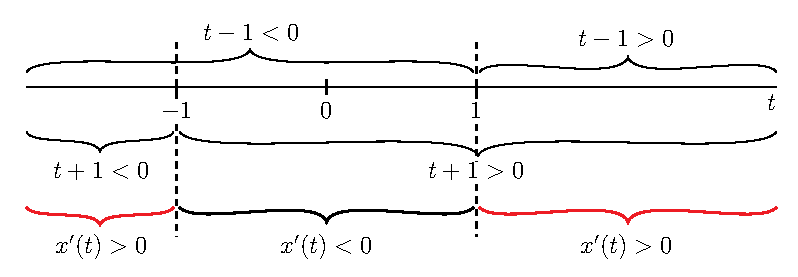
\includegraphics{speedD}
\end{center}
\end{efig}
It is now easy to put together a mental image of your trajectory.
\begin{itemize}
\item For $t$ large and negative (i.e. far in the past), $x(t)$ is large
and negative and $v(t)$ is large and positive. For example\footnote{Notice here we are
using the fact that when $t$ is very large $t^3$ is much bigger than $t^2$ and $t^1$.
So we can approximate the value of the polynomial $x(t)$ by the largest term --- in
this case $t^3$. We can do similarly with $v(t)$ --- the largest term is $3t^2$.}, when
$t=-10^6$, $x(t)\approx t^3=- 10^{18}$ and $v(t)\approx  3t^2 = 3\cdot 10^{12}$.
So you are moving quickly to the right.

\item For $t<-1$, $v(t)=x'(t)>0$ so that $x(t)$ is increasing and you are moving
to the right.

\item At $t=-1$, $v(-1)=0$ and you have come to a halt at
position $x(-1)=(-1)^3-3(-1)+2=4$.

\item For $-1<t<1$, $v(t)=x'(t)<0$ so that $x(t)$ is decreasing and you are moving
to the left.

\item At $t=+1$, $v(1)=0$ and you have again come to a halt, but now at
position $x(1)=1^3-3+2=0$.

\item For $t>1$, $v(t)=x'(t)>0$ so that $x(t)$ is increasing and you are
again moving to the right.

\item For $t$ large and positive (i.e. in the far future), $x(t)$ is large
and positive and $v(t)$ is large and positive. For example\footnote{We are making a
similar rough approximation here.}, when $t=10^6$, $x(t)\approx t^3= 10^{18}$ and
$v(t)\approx  3t^2 = 3\cdot 10^{12}$. So you are moving quickly to the right.

\end{itemize}
Here is a sketch of the graphs of $x(t)$ and $v(t)$. The heavy lines in the graphs
indicate when you are moving to the right --- that is where $v(t)=x'(t)$ is positive.

\begin{efig}
\begin{center}
   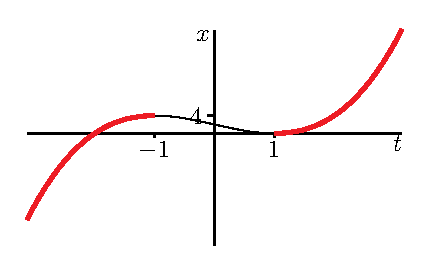
\includegraphics{speedB}
   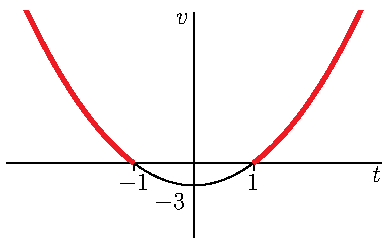
\includegraphics{speedA}
\end{center}
\end{efig}

And here is a schematic picture of the whole trajectory.

\begin{efig}
\begin{center}
   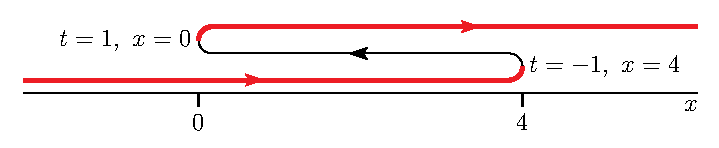
\includegraphics{speedC}
\end{center}
\end{efig}

\end{eg}

\begin{eg}\label{eg:fallingBallB}
In this example we are going to figure out how far a body falling from rest will fall in
a given time period.
\begin{itemize}
 \item We should start by defining some variables and their units. Denote
  \begin{itemize}
   \item time in seconds by $t$,
   \item mass in kilograms by $m$,
  \item distance fallen (in metres) at time $t$ by $s(t)$, velocity (in m/sec) by
  $v(t)=s'(t)$ and acceleration (in m/sec$^2$) by $a(t)=v'(t)=s''(t)$.
  \end{itemize}
It makes sense to choose a coordinate system so that the body starts to fall at $t=0$.

\item We will use Newton's second law of motion
\begin{align*}
\text{the force applied to the body at time $t$} = m \cdot a(t).
\end{align*}
together with the assumption that the only force acting on the body is gravity (in
particular, no air resistance). Note that near the surface of the Earth,
\begin{align*}
\text{the force due to gravity acting on a body of mass $m$} &= m \cdot g.
\end{align*}
The constant $g$, called the acceleration of gravity\footnote{It is also called the
standard acceleration due to gravity or standard gravity. For those of you who prefer
imperial units (or US customary units), it is about $32$ ft/sec$^2$, $77165$
cubits/minute$^2$, or $631353$ furlongs/hour$^2$.}, is about 9.8m/sec$^2$.

\item Since the body is falling from rest, we know that its initial velocity is zero.
That is
\begin{align*}
  v(0) &= 0.
\end{align*}
Newton's second law then implies that
\begin{align*}
m\cdot a(t) &= \text{force due to gravity} \\
  m \cdot v'(t) &= m \cdot g & \text{ cancel the $m$} \\
  v'(t) &=g
\end{align*}

\item In order to find the velocity, we need to find a function of $t$ whose derivative
is constant. We are simply going to guess such a function and then we will verify that our
guess has all of the desired properties. It's easy to guess a function whose derivative is
the constant $g$.  Certainly $gt$ has the correct derivative. So does
\begin{align*}
    v(t) = gt + c
\end{align*}
for any constant $c$. One can then verify\footnote{While it is clear that this satisfies
the equation we want, it is less clear that it is the only function that
works. To see this, assume that there are two functions $f(t)$ and $h(t)$ which both
satisfy $v'(t)=g$. Then $f'(t)=h'(t) = g$ and so $f'(t)-h'(t) = 0$. Equivalently
\begin{align*}
  \diff{}{t}\left( f(t)-h(t) \right) &= 0.
\end{align*}
The only function whose derivative is zero everywhere is the constant function (see
Section~\ref{sec mvt} and Theorem~\ref{cor:DIFFmvtcons}). Thus $f(t)-h(t) =
\text{constant}$. So all the functions that satisfy $v'(t)=g$ must be of the form $gt +
\text{constant}$.
} that $v'(t)=g$. Using the fact that $v(0)=0$ we must then have $c=0$ and so
\begin{align*}
  v(t) &= gt.
\end{align*}

\item Since velocity is the derivative of position, we know that
\begin{align*}
  s'(t) &= v(t) = g \cdot t.
\end{align*}
To find $s(t)$ we are again going to guess and check. It's not hard to see that we can use
\begin{align*}
  s(t) &= \frac{g}{2} t^2 + c
\end{align*}
where again $c$ is some constant. Again we can verify that this works
simply by differentiating\footnote{To show that any solution of $s'(t)=gv$
must be of this form we can use the same reasoning we used to get $v(t) = gt +
\text{constant}$.}. Since we have defined $s(t)$ to be the distance fallen, it follows
that $s(0)=0$ which in turn tells us that $c = 0$. Hence
\begin{align*}
  s(t) &= \frac{g}{2} t^2 & \text{but $g=9.8$, so}\\
  &= 4.9 t^2,
\end{align*}
which is exactly the $s(t)$ used way back in Section~\ref{sec velocity}.
\end{itemize}


\end{eg}

Let's now do a similar but more complicated example.

\begin{eg}\label{eg:braking}
A car's brakes can decelerate the car at 64000$\textrm{km/hr}^2$.
How fast can the car be driven if it must be able to stop within a distance
of 50m?

\soln Before getting started, notice that there is a small ``trick'' in this problem
--- several quantities are stated but their units are different. The acceleration is
stated in kilometres per hour$^2$, but the distance is stated in metres. Whenever we come
across a ``real world'' problem\footnote{Well --- ``realer world'' would perhaps be a
betterer term.} we should be careful of the units used.

\begin{itemize}
 \item We should first define some variables and their units. Denote
\begin{itemize}
 \item time (in hours) by $t$,
 \item the position of the car (in kilometres) at time $t$ by $x(t)$, and
 \item the velocity (in kilometres per hour) by is $v(t)$.
\end{itemize}
  We can also choose a coordinate system such that $x(0)=0$ and the car starts
  braking at time $t=0$.

\item Now let us rewrite the information in the problem in terms of these variables.
\begin{itemize}
 \item We are told that, at maximum braking, the acceleration $v'(t)=x''(t)$ of the car
is $-64000$.
 \item We need to determine the maximum initial velocity $v(0)$ so that the stopping
distance is at most $50m = 0.05km$ (being careful with our units). Let us call the
stopping distance $x_{stop}$ which is really $x(t_{stop})$ where $t_{stop}$ is the
stopping time.
\end{itemize}

\item In order to determine $x_{stop}$ we first need to determine $t_{stop}$, which we
will do by assuming maximum braking from a, yet to be determined, initial velocity of
$v(0)=q$ m/sec.

\item Assuming that the car undergoes a constant acceleration at this maximum braking
power, we have
\begin{align*}
  v'(t) &= -64000
\end{align*}
This equation is very similar to the ones we had to solve in
Example~\ref{eg:fallingBallB} just above.

As we did there\footnote{Now is a good time to go back and have a read of that example.},
we are going to just guess $v(t)$. First, we just guess one function whose derivative is
$-64000$, namely $-64000 t$. Next we observe that, since the derivative of a constant is
zero, any function of the form
\begin{align*}
  v(t) = -64000\,t + c
\end{align*}
with constant $c$, has the correct derivative. Finally, the requirement that the initial
velocity $v(0)=q$" forces $c=q$, so
\begin{align*}
  v(t) = q - 64000\,t
\end{align*}

\item From this we can easily determine the stopping time $t_{stop}$, when the initial
velocity is $q$, since this is just when $v(t) = 0$:
\begin{align*}
  0 = v(t_{stop}) &= q-64000 \cdot t_{stop} & \text{ and so}\\
  t_{stop} &= \frac{q}{64000}.
\end{align*}
\item Armed with the stopping time, how do we get at the stopping distance?  We need to
find the formula satisfied by $x(t)$. Again (as per Example~\ref{eg:fallingBallB}) we
make use of the fact that
\begin{align*}
x'(t) &= v(t) = q - 64000t.
\end{align*}
So we need to guess a function $x(t)$ so that $x'(t) = q-64000 t$. It is not hard to see
that
\begin{align*}
  x(t) &= qt - 32000t^2 + \text{constant}
\end{align*}
works. Since we know that $x(0)=0$, this constant is just zero and
\begin{align*}
  x(t) &= qt - 32000 t^2.
\end{align*}

\item We are now ready to compute the stopping distance (in terms of the, still yet to be
determined, initial velocity $q$):
\begin{align*}
  x_{stop} &= x(t_{stop}) = q t_{stop} - 32000 t_{stop}^2 \\
  &= \frac{q^2}{64000} - \frac{32000 q^2}{64000^2} \\
  &= \frac{q^2}{64000} \left(1 - \frac{1}{2} \right) \\
  &= \frac{q^2}{2 \times 64000}
\end{align*}
Notice that the stopping distance is a quadratic function of the initial velocity --- if
you go twice as fast, you need four times the distance to stop.

\item But we are told that the stopping distance must be less than $50m = 0.05km$. This
means that
\begin{align*}
  x_{stop} = \frac{q^2}{2 \times 64000} &\leq \frac{5}{100}  \\
    q^2 &\leq \frac{2 \times 64000 \times 5}{100} = \frac{64000 \times 10}{100} = 6400
\end{align*}
Thus we must have $q \leq 80$. Hence the initial velocity can be no greater than $80km/h$.
\end{itemize}

\end{eg}

%%%%%%%%%%%%%%%%%%%%%%%%%%
\section{Related Rates}\label{sec rrates}
%%%%%%%%%%%%%%%%%%%%%%%%%%

Consider the following problem
\begin{quote}
 A spherical balloon is being inflated at a rate of $13cm^3/sec$. How fast is
the radius changing when the balloon has radius $15cm$?
\end{quote}
There are several pieces of information in the statement:
\begin{itemize}
 \item The balloon is spherical
 \item The volume is changing at a rate of $13cm^3/sec$ --- so we need variables
for volume (in $cm^3$) and time (in $sec$). Good choices are $V$ and $t$.
\item We are asked for the rate at which the radius is changing --- so we need
a variable for radius and units. A good choice is $r$, measured in $cm$ ---
since volume is measured in $cm^3$.
\end{itemize}
Since the balloon is a sphere we know\footnote{If you don't know the formula
for the volume of a sphere, now is a good time to revise by looking at
Appendix~\ref{sec volumes}.} that
\begin{align*}
  V &= \frac{4}{3} \pi r^3
\end{align*}
Since both the volume and radius are changing with time, both $V$ and $r$ are
implicitly functions of time; we could really write
\begin{align*}
  V(t) &= \frac{4}{3}\pi r(t)^3.
\end{align*}
We are told the rate at which the volume is changing and we need to find the
rate at which the radius is changing. That is, from a knowledge of
$\diff{V}{t}$, find the related rate\footnote{Related rate problems are problems in which
you are given the rate of change of one quantity and are to determine the rate of
change of another, related, quantity.} $\diff{r}{t}$.

In this case, we can just differentiate our equation by $t$ to get
\begin{align*}
  \diff{V}{t} &= 4 \pi r^2 \diff{r}{t}
\intertext{This can then be rearranged to give}
  \diff{r}{t} &= \frac{1}{4\pi r^2} \diff{V}{t}.
\end{align*}
Now we were told that $\diff{V}{t} = 13$, so
\begin{align*}
  \diff{r}{t} &= \frac{13}{4\pi r^2}.
\end{align*}
We were also told that the radius is $15cm$, so at that moment in time
\begin{align*}
  \diff{r}{t} &= \frac{13}{\pi 4 \times 15^2}.
\end{align*}

This is a very typical example of a related rate problem. This section is really
just a collection of problems, but all will follow a similar pattern.
\begin{itemize}
 \item The statement of the problem will tell you quantities that must be
related (above it was volume, radius and, implicitly, time).
\item Typically a little geometry (or some physics or\dots) will allow you to
relate these quantities (above it was the formula that links the volume of a
sphere to its radius).
\item Implicit differentiation will then allow you to link the rate of change
of one quantity to another.
\end{itemize}

Another balloon example
\begin{eg}
Consider a helium balloon rising vertically from a fixed point 200m away from
you. You are trying to work out how fast it is rising. Now --- computing the
velocity directly is difficult, but you can measure angles. You observe that
when it is at an angle of $\pi/4$ its angle is changing by $0.05$ radians per
second.

\begin{itemize}
 \item Start by drawing a picture with the relevant variables
\begin{efig}
\begin{center}
 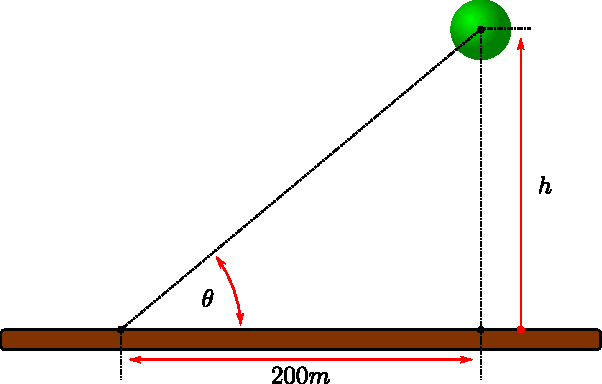
\includegraphics[height=5cm]{extra/balloon1}
\end{center}
\end{efig}
\item So denote the angle to be $\theta$ (in radians), the height of the balloon (in m)
by $h$ and time (in seconds) by $t$. Then trigonometry tells us
\begin{align*}
  h &= 200 \cdot \tan \theta
\end{align*}
\item Differentiating allows us to relate the rates of change
\begin{align*}
  \diff{h}{t} &= 200 \sec^2 \theta \cdot \diff{\theta}{t}
\end{align*}
\item We are told that when $\theta =\pi/4$ we observe $\diff{\theta}{t} =
0.05$, so
\begin{align*}
  \diff{h}{t} &= 200 \cdot \sec^2(\pi/4) \cdot 0.05 \\
  &= 200 \cdot 0.05 \cdot \left( \sqrt{2} \right)^2 \\
  &= 200 \cdot \frac{5}{100} \cdot 2
  &= 20 m/s
\end{align*}
\item So the balloon is rising at a rate of 20m/s.
\end{itemize}

\end{eg}


The following problem is perhaps \emph{the} classic related rate problem.
\begin{eg}
 A 5m ladder is leaning against a wall. The floor is quite slippery and the
base of the ladder slides out from the wall at a rate of $1m/s$. How fast is
the top of the ladder sliding down the wall when the base of the ladder is 3m
from the wall?

\begin{itemize}
 \item A good first step is to draw a picture stating all relevant quantities.
This will also help us define variables and units.
\begin{efig}
\begin{center} 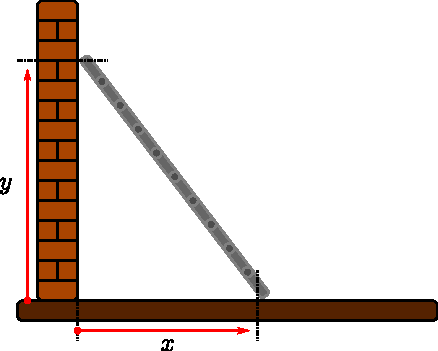
\includegraphics[height=5.5cm]{extra/ladder1}
\end{center}

\end{efig}
 \item So now define $x(t)$ to be the distance between the bottom of the ladder and the
wall, at time $t$, and let $y(t)$ be the distance between the top of the ladder and the
ground at time $t$. Measure time in seconds, but both distances in meters.

\item We can relate the quantities using Pythagoras:
\begin{align*}
  x^2 + y^2 &= 5^2
\end{align*}
\item Differentiating with respect to time then gives
\begin{align*}
  2x \diff{x}{t} + 2y \diff{y}{t} &= 0
\end{align*}
\item We know that $\diff{x}{t} = 1$ and $x=3$, so
\begin{align*}
  6 \cdot 1 + 2y \diff{y}{t} &= 0
\end{align*}
but we need to determine $y$ before we can go further. Thankfully we know that
$x^2+y^2=25$ and $x=3$, so $y^2=25-9=16$ and\footnote{Since the ladder
isn't buried in the ground, we can discard the solution $y=-4$.} so $y=4$.
\item So finally putting everything together
\begin{align*}
  6 \cdot 1 + 8 \diff{y}{t} &= 0 \\
  \diff{y}{t} &= - \frac{3}{4} m/s.
\end{align*}
Thus the top of the ladder is sliding towards the floor at a rate of $3/4 m/s$.
\end{itemize}

\end{eg}

The next example is complicated by the rates of change being stated not just as ``the
rate of change per unit time'' but instead being stated as ``the percentage rate of
change per unit time''. If a quantity $f$ is changing with rate $\diff{f}{t}$, then we can
say that
\begin{quote}
 $f$ is changing at a rate of $\ds 100 \cdot \frac{\diff{f}{t}}{f}$ percent.
\end{quote}

Thus if, at time $t$, $f$ has rate of change $r\%$, then
\begin{align*}
    100\frac{f'(t)}{f(t)}=r
    \implies f'(t) =\frac{r}{100} f(t)
\end{align*}
so that if $h$ is a very small time increment
\begin{align*}
    \frac{f(t+h) - f(t)}{h} \approx \frac{r}{100} f(t)
    \implies f(t+h) \approx f(t) + \frac{rh}{100} f(t)
\end{align*}
That is, over a very small time interval $h$, $f$ increases
by the fraction $\frac{rh}{100}$ of its value at time $t$.

So armed with this, let's look at the problem.
\begin{eg}\label{eg:percentGrowth}
The quantities $P,\ Q$ and $R$ are functions of time and are related
by the equation $R=PQ$. Assume that $P$ is increasing instantaneously at
the rate of $8\%$ per year (meaning that $100\frac{P'}{P}=8$) and that
$Q$ is decreasing instantaneously at the rate of $2\%$ per year (meaning
that $100\frac{Q'}{Q}=-2$).
Determine the percentage rate of change for $R$.

\soln This one is a little different --- we are given the variables and
the formula, so no picture drawing or defining required. Though we do need to
define a time variable --- let $t$ denote time in years.
\begin{itemize}
 \item Since $R(t) = P(t)\cdot Q(t)$ we can differentiate with respect to $t$ to get
\begin{align*}
  \diff{R}{t} &= P Q' + Q P'
\end{align*}
 \item But we need the percentage change in $R$, namely
\begin{align*}
  100 \frac{R'}{R} &= 100 \frac{PQ' +QP'}{R}
\intertext{but $R = PQ$, so rewrite it as}
  &= 100 \frac{PQ' +QP'}{PQ}  \\
  &= 100 \frac{PQ'}{PQ} + 100 \frac{QP'}{PQ} \\
  &= 100 \frac{Q'}{Q} + 100 \frac{P'}{P}
\end{align*}
so we have stated the instantaneous percentage rate of change
in $R$ as the sum of the percentage rate of change in $P$ and $Q$.
\item We know the percentage rate of change of $P$ and $Q$, so
\begin{align*}
  100 \frac{R'}{R} &= -2 + 8 =6
\end{align*}
That is, the instantaneous percentage rate of change of $R$ is 6\% per year.
\end{itemize}
\end{eg}

Yet another falling object example.
\begin{eg}\label{eg:fallingBall}
A ball is dropped from a height of $49$m above level ground. The
height of the ball at time $t$ is $h(t)=49-4.9 t^2$ m. A light,
which is also $49$m above the ground, is $10$m to the left of
the ball's original position. As the ball descends, the shadow
of the ball caused by the light moves across the ground. How
fast is the shadow moving one second after the ball is dropped?

\soln There is quite a bit going on in this example, so read carefully.
\begin{itemize}
 \item First a diagram; the one below is perhaps a bit over the top.
\begin{efig}
\begin{center}
%     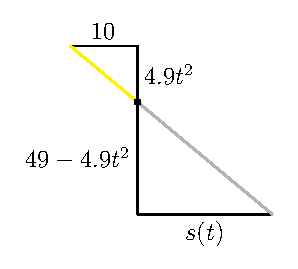
\includegraphics{ballShadow}
    \includegraphics{extra/falling_ball}
\end{center}
\end{efig}
\item Let's call $s(t)$ the distance from the shadow to the point
on the ground directly underneath the ball.

\item By similar triangles we see that
\begin{align*}
\frac{4.9 t^2}{10}=\frac{49-4.9 t^2}{s(t)}
\end{align*}
We can then solve for $s(t)$ by just multiplying both sides by
$\frac{10}{4.9 t^2}s(t)$. This gives
\begin{align*}
s(t)=10\frac{49-4.9 t^2}{4.9 t^2}=\frac{100}{t^2}-10
\end{align*}
\item Differentiating with respect to $t$ will then give us the rates,
\begin{align*}
s'(t)=-2\frac{100}{t^3}
\end{align*}
\item So, at $t=1$, $s'(1)=-200$m/sec. That is, the shadow is moving
to the left at $200$m/sec.
\end{itemize}

\end{eg}

A more nautical example.
\begin{eg}
Two boats spot each other in the ocean at midday --- Boat $A$ is 15km west of
Boat $B$. Boat $A$ is travelling east at 3km/h and boat $B$ is travelling north at 4km/h.
At 3pm how fast is the distance between the boats changing.
\begin{itemize}
 \item First we draw a picture.
\begin{efig}
\begin{center}
 \includegraphics[height=5.5cm]{extra/boats1}
\end{center}
\end{efig}
\item Let $x(t)$ be the distance at time $t$, in km, from boat $A$ to the original
position of boat $B$ (i.e. to the position of boat $B$ at noon). And let $y(t)$ be the
distance at time $t$, in km, of boat $B$ from its original position. And let $z(t)$ be the
distance between the two boats at time $t$.

\item Additionally we are told that $x'=-3$ and $y'=4$ --- notice that $x' <0$ since that
distance is getting smaller with time, while $y'>0$ since that distance is
increasing with time.

\item Further at $3pm$ boat $A$ has travelled 9km towards the original position of boat
$B$, so $x=15-9 = 6$, while boat $B$ has travelled 12km away from its original position,
so $y=12$.

\item The distances $x,y$ and $z$ form a right-angled triangle, and Pythagoras
tells us that
\begin{align*}
  z^2 &= x^2 + y^2.
\end{align*}
At 3pm we know $x=6,y=12$ so
\begin{align*}
  z^2 &= 36 + 144 = 180 \\
  z&= \sqrt{180} = 6\sqrt{5}.
\end{align*}

\item Differentiating then gives
\begin{align*}
  2z \diff{z}{t} &= 2x \diff{x}{t} + 2y \diff{y}{t} \\
  &= 12 \cdot (-3) + 24 \cdot(4) \\
  &= 60.
\intertext{Dividing through by $2z = 12\sqrt{5}$ then gives}
\diff{z}{t} &= \frac{60}{12\sqrt{5}} = \frac{5}{\sqrt{5}} = \sqrt{5}
\end{align*}
So the distance between the boats is increasing at $\sqrt{5} km/h$.
\end{itemize}
\end{eg}

One last one before we move on to another topic.
\begin{eg}\label{eg:fuel}
\begin{tabular}{m{0.75\textwidth}m{0.25\textwidth}}
Consider a cylindrical fuel tank of radius $r$ and length $L$ (in some appropriate units)
that is lying on its side. Suppose that fuel is being pumped into the tank at
a rate $q$. At what rate is the fuel level rising?
%
&
%
\quad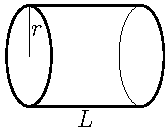
\includegraphics{fuel1}
\end{tabular}


\soln If the tank were vertical everything would be much easier. Unfortunately the tank
is on its side, so we are going to have to work a bit harder to establish the relation
between the depth and volume. Also notice that we have not been supplied with units for
this problem --- so we do not need to state the units of our variables.

\begin{itemize}
 \item Again --- draw a picture. Here is an end view of the tank; the shaded part of the
circle  is filled with fuel.

\begin{efig}
\begin{center}
    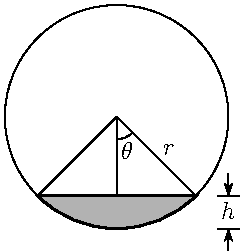
\includegraphics{fuel2}
\end{center}
\end{efig}

\item Let us denote by $V(t)$ the volume of fuel in the tank at time
$t$ and by $h(t)$ the fuel level at time $t$.

\item We have been told that $V'(t)=q$ and have been asked to determine $h'(t)$. While it is
possible to do so by finding a formula relating $V(t)$ and $h(t)$, it turns out to be
quite a bit easier to first find a formula relating $V$ and the angle $\theta$ shown in
the end view. We can then translate this back into a formula in terms of $h$ using the
relation
\begin{align*}
  h(t) &= r - r\cos \theta(t).
\end{align*}
Once we know $\theta'(t)$, we can easily obtain $h'(t)$ by differentiating the above
equation.

\item The computation that follows below gets a little involved in places, so we will
drop the ``$(t)$'' on the variables $V,h$ and $\theta$. The reader must never forget that
these three quantities are really functions of time, while $r$ and $L$ are constants that
do not depend on time.

\item The volume of fuel is $L$ times the cross--sectional area filled by
the fuel. That is,
\begin{align*}
  V=L\times\textrm{Area} \big(\smash{\raisebox{-0.2\height}{
                                      \!
\includegraphics{fuel3}\!
                                                        }}\big)
\end{align*}
While we do not have a canned formula for the area of a chord of a circle
like this, it is easy to express the area of the chord in terms of two areas that we can
compute.
\begin{align*}
  V=L\times\textrm{Area} \big(\smash{\raisebox{-0.2\height}{
                                      \!
\includegraphics{fuel3}\!
                                                        }}\big)
  =L\times\bigg[\textrm{Area} \bigg(\raisebox{-0.5\height}{
                                    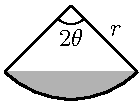
\includegraphics[height=0.7in]{fuel4}
                                                        }\bigg)
    -\textrm{Area}  \bigg(\raisebox{-0.4\height}{
                                    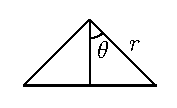
\includegraphics[height=0.5in]{fuel5}
                                                        }\bigg)\bigg]
\end{align*}
\begin{itemize}
 \item The piece of pie \raisebox{-0.5\height}{
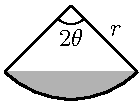
\includegraphics[height=0.7in]{fuel4}} is the fraction $\tfrac{2\theta}{2\pi}$ of the full
circle, so its area is $\tfrac{2\theta}{2\pi}\pi r^2=\theta r^2$.

\item The triangle \raisebox{-0.4\height}{
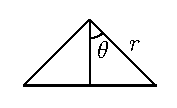
\includegraphics[height=0.5in]{fuel5}}  as height $r\cos\theta$ and base $2r\sin\theta$
and hence has area $\frac{1}{2}(r\cos\theta)(2r\sin\theta)=r^2\sin\theta\cos\theta =
\frac{r^2}{2} \sin(2\theta)$, where we have used a double-angle formula (see
Appendix~\ref{sec must deriv}).
\end{itemize}
Subbing these two areas into the above expression for $V$ gives
\begin{align*}
  V & = L\times\left[\theta r^2- \frac{r^2}{2}\sin2\theta\right]
  = \frac{Lr^2}{2} \big[2\theta-\sin2\theta \big]
\end{align*}
Oof!
\item Now we can differentiate to find the rate of change. Recalling that $V=V(t)$ and
$\theta=\theta(t)$, while $r$ and $L$ are constants,
\begin{align*}
  V'
  &=\frac{Lr^2}{2} \left[ 2\theta' - 2\cos2\theta \cdot \theta' \right]\\
  &= Lr^2 \cdot \theta' \cdot \left[1 - \cos2\theta \right]
%
%   &=2\theta'(t)Lr^2\sin^2\theta(t)
\end{align*}
Solving this for $\theta'$ and using $V'=q$ gives
\begin{align*}
  \theta' &= \frac{q}{Lr^2 (1-\cos2\theta)}
\end{align*}
This is the rate at which $\theta$ is changing, but we need the rate at which $h$ is
changing. We get this from
\begin{align*}
  h &= r - r\cos \theta & \text{differentiating this gives}\\
  h' &= r\sin\theta \cdot \theta'
\end{align*}
Substituting our expression for $\theta'$ into the expression for $h'$ gives
\begin{align*}
  h' &= r\sin\theta \cdot \frac{q}{Lr^2 (1-\cos2\theta)}
\end{align*}

\item We can clean this up a bit more --- recall more double-angle
formulas\footnote{Take another look at Appendix~\ref{sec must deriv}.}
\begin{align*}
  h'
&= r\sin\theta \cdot \frac{q}{Lr^2 (1-\cos2\theta)} & \text{substitute $\cos2\theta =
1-2\sin^2\theta$}\\
&= r\sin\theta \cdot \frac{q}{Lr^2 \cdot 2\sin^2\theta} & \text{now cancel $r$'s and a $\sin\theta$}\\
&= \frac{q}{2Lr\sin\theta}
\end{align*}

\item But we can clean this up even more --- instead of writing this rate in terms of
$\theta$ it is more natural to write it in terms of $h$ (since the initial problem is
stated in terms of $h$). From the triangle
\begin{efig}
\begin{center}
       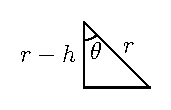
\includegraphics{fuel6}
\end{center}
\end{efig}
and Pythagoras we have
\begin{align*}
  \sin\theta =\frac{\sqrt{r^2-(r-h)^2}}{r}=\frac{\sqrt{2rh-h^2}}{r}
\end{align*}
and hence
\begin{align*}
  h' = \frac{q}{2L\sqrt{2rh-h^2}}.
\end{align*}

\item As a check, notice that $h'$ becomes undefined when $h<0$ and also when $h>2r$,
because then the argument of the square root in the denominator is negative. Both make
sense --- the fuel level in the tank must obey $0\le h\le 2r$.
\end{itemize}

\end{eg}



%%%%%%%%%%%%%%%%%%%%%%%%%%%%%%%%%%%%%%%%%%%%%%%%%%%%%%%%%%%%%%%%%
\longsection{Exponential Growth and Decay --- a First Look at Differential
Equations}{Exponential growth and decay}\label{sec:ExpGthDecay}
%%%%%%%%%%%%%%%%%%%%%%%%%%%%%%%%%%%%%%%%%%%%%%%%%%%%%%%%%%%%%%%%%
A differential equation is an equation for an unknown function
that involves the derivative of the unknown function. For example,
Newton's law of cooling says:
\begin{quote}
    The rate of change of temperature of an object is proportional
    to the difference in temperature between the object and its
    surroundings.
\end{quote}
We can write this more mathematically using a differential equation --- an equation for
the unknown function $T(t)$ that also involves its derivative $\diff{T}{t}(t)$.
If we denote by $T(t)$ the temperature of the
object at time $t$ and by $A$ the temperature of its surroundings, Newton's law of
cooling says that there is some constant of proportionality,
$K$, such that
% \begin{impeqn}[Newton's law of cooling]
\begin{align*}
    \diff{T}{t}(t) &= K\big[T(t)-A\big]
\end{align*}
% \end{impeqn}


Differential equations play a central role in modelling a huge number of
different phenomena, including the motion of particles, electromagnetic
radiation, financial options, ecosystem populations and nerve action potentials.
Most universities offer half a dozen different undergraduate courses on various
aspects of differential equations. We are barely going to scratch the surface
of the subject. At this point we are going to restrict ourselves
to a few very simple differential equations for which we can just
guess the solution. In particular, we shall learn how to
solve systems obeying Newton's law of cooling in Section~\ref{sec:newtonCooling},
below. But first, here is another slightly simpler example.




%%%%%%%%%%%%%%%%%%%%%%%%%%%%%%%%%%%%%%%%%%%%%%%%%%%%%%%%%%%%%%%%%
\subsection{Carbon Dating}\label{ssec carbon}
%%%%%%%%%%%%%%%%%%%%%%%%%%%%%%%%%%%%%%%%%%%%%%%%%%%%%%%%%%%%%%%%%
Scientists can determine the age of objects containing organic material by a
method called {\it carbon dating} or {\it radiocarbon dating}\footnote{Willard
Libby, of Chicago University was awarded the Nobel Prize in Chemistry in 1960,
for developing radiocarbon dating.}. Cosmic rays hitting the atmosphere convert
nitrogen into a radioactive isotope of carbon, ${}^{14}C$, with a half--life of
about 5730 years\footnote{A good question to ask yourself is ``How can a
scientist (who presumably doesn't live 60 centuries) measure this quantity?''
One way exploits the little piece of calculus we are about to discuss.}.
Vegetation absorbs carbon dioxide from the atmosphere through photosynthesis and
animals acquire ${}^{14}C$ by eating plants. When a plant or animal dies, it
stops replacing its carbon and the amount of ${}^{14}C$ begins to decrease
through radioactive decay. More precisely, let $Q(t)$ denote the amount of
${}^{14}C$ in the plant or animal $t$ years after it dies. The number of
radioactive decays per unit time, at time $t$, is proportional to the amount of
${}^{14}C$ present at time $t$, which is $Q(t)$. Thus
\begin{impeqn}[Radioactive decay]\label{eq:carbonDating}
\begin{align*}
\diff{Q}{t}(t) &=-k Q(t)
\end{align*}
\end{impeqn}
\noindent Here $k$ is a constant of proportionality that is determined
by the half--life. We shall explain what half-life is and also determine
the value of $k$ in Example \ref{eg:carbonDatingHalfLife}, below. Before we do so, let's
think about the sign in equation~\eqref{eq:carbonDating}.
\begin{itemize}
 \item Recall that $Q(t)$ denotes  a quantity, namely the amount of ${}^{14}C$ present at
time $t$. There cannot be a negative amount of ${}^{14}C$, nor can this quantity be zero
(otherwise we wouldn't use carbon dating, so we must have $Q(t)> 0$.
\item As the time $t$ increases, $Q(t)$ decreases, because ${}^{14}C$ is being
continuously converted into ${}^{14}N$ by radioactive decay\footnote{
The precise transition is ${}^{14}C\rightarrow {}^{14}N+ e^- + \bar{\nu}_e$
where $e^-$ is an electron and $\bar{\nu}_e $ is an electron neutrino.}. Thus
$\diff{Q}{t}(t)< 0$.

\item The signs $Q(t)> 0$ and $\diff{Q}{t}(t)< 0$
are consistent with equation~\eqref{eq:carbonDating} provided the constant of
proportionality $k>0$.

\item In equation~\eqref{eq:carbonDating}, we chose to call the constant of
proportionality
``$-k$''. We did so in order to make $k>0$. We could just as well have chosen to
call the constant of proportionality ``$K$''.  That is, we could have replaced
equation~\eqref{eq:carbonDating} by $\diff{Q}{t}(t)=K Q(t)$. The constant of
proportionality $K$ would have to be negative, (and $K$ and $k$ would be
related by  $K=-k$).

\end{itemize}


Now, let's guess some solutions to equation~\eqref{eq:carbonDating}. We
wish to guess a function $Q(t)$ whose derivative is just a constant times
itself. Here is a short table of derivatives. It is certainly not complete,
but it contains the most important derivatives that we know.
%\renewcommand{\arraystretch}{1.3}
%\begin{center}
%     \begin{tabular}{|c|c|}
%          \hline $F(t)$&  $\diff{}{t}F(t)$ \\ \hline\hline
%                 $1$  &   $0$ \\ \hline
%                 $t^a$&  $at^{a-1}$ \\ \hline
%                 $\sin t$&  $\cos t$ \\ \hline
%                 $\cos t$&  $-\sin t$ \\ \hline
%                 $\tan t$&  $\sec^2 t$ \\ \hline
%                 $e^t$&  $e^t$ \\ \hline
%                 $\log t$&  $\frac{1}{t}$ \\ \hline
%                 $\arcsin t$ & $\frac{1}{\sqrt{1-t^2}}$ \\ \hline
%                 $\arctan t$ & $\frac{1}{1+t^2}$ \\ \hline
%     \end{tabular}
%\end{center}
%\renewcommand{\arraystretch}{1.0}
\renewcommand{\arraystretch}{1.3}
\begin{center}
     \begin{tabular}{|c||c|c|c|c|c|c|c|c|c|}
          \hline
                  $F(t)$ &           $1$ &  $t^a$ &     $\sin t$ & $\cos t$
                  & $\tan t$ & $e^t$ & $\log t$
                  & $\arcsin t$ & $\arctan t$
           \\ \hline
                  $\diff{}{t}F(t)$ & $0$ & $at^{a-1}$ & $\cos t$ & $-\sin t$
                  &  $\sec^2 t$ & $e^t$ & $\frac{1}{t}$
                  & $\frac{1}{\sqrt{1-t^2}}$ & $\frac{1}{1+t^2}$
           \\ \hline
     \end{tabular}
\end{center}
\renewcommand{\arraystretch}{1.0}
There is exactly one function in this table whose derivative is just a
(nonzero) constant times itself. Namely, the derivative of $e^t$ is exactly
$e^t = 1\times e^t$. This is almost, but not quite what we want. We want
the derivative of $Q(t)$ to be the constant $-k$ (rather than the constant
$1$) times $Q(t)$. We want the derivative to ``pull a constant'' out of
our guess. That is exactly what happens when we differentiate $e^{at}$,
where $a$ is a constant. Differentiating gives
\begin{align*}
\diff{}{t}e^{at} = a e^{at}
\end{align*}
i.e. ``pulls the constant $a$ out of $e^{at}$''.


We have succeeded in guessing a single function, namely $e^{-kt}$, that obeys
equation~\eqref{eq:carbonDating}. Can we guess any other solutions? Yes.
If $C$ is any constant, $Ce^{-kt}$ also obeys equation~\eqref{eq:carbonDating}:
\begin{align*}
\diff{}{t}(Ce^{-kt}) = C\diff{}{t}e^{-kt} = Ce^{-kt}(-k) = -k (Ce^{-kt})
\end{align*}
You can try guessing some more solutions, but you won't find any,
because with a little trickery we can prove that a function $Q(t)$
obeys equation~\eqref{eq:carbonDating} if and only if $Q(t)$ is of the form
$Ce^{-kt}$, where $C$ is some constant.


The trick\footnote{
Notice that is very similar to what we needed in Example~\ref{eg:fallingBallB},
except that here the constant is multiplicative rather than additive. That is
$const \times f(t)$ rather than $const + f(t)$.
} is to imagine that $Q(t)$ is any (at this stage, unknown) solution to
\eqref{eq:carbonDating} and to compare $Q(t)$ and our known solution $e^{-kt}$
by studying the ratio $Q(t)/e^{-kt}$. We will show that $Q(t)$ obeys
\eqref{eq:carbonDating} if and only if the ratio $Q(t)/e^{-kt}$ is a constant,
i.e. if and only if the derivative of the ratio is zero. By the product rule
\begin{align*}
\diff{}{t}\big[Q(t)/e^{-kt}\big]=
\diff{}{t}\big[e^{kt}Q(t)\big]
=ke^{kt} Q(t)+e^{kt}Q'(t)
\end{align*}
Since $e^{kt}$ is never $0$, the right hand side is zero if and only if
$k Q(t)+Q'(t)=0$; that is $Q'(t)=-kQ(t)$. Thus
\begin{align*}
\diff{}{t}Q(t) = -k Q(t)
\iff
\diff{}{t}\big[Q(t)/e^{-kt}\big]
=0
\end{align*}
as required.

We have succeed in finding all functions that obey \eqref{eq:carbonDating}.
That is, we have found the general solution to \eqref{eq:carbonDating}.
This is worth stating as a theorem.
\begin{theorem}\label{thm:growthDEsoln}
A differentiable function $Q(t)$ obeys the differential equation
\begin{align*}
\diff{Q}{t}(t)=-k Q(t)
\end{align*}
if and only if there is a constant $C$ such that
\begin{align*}
Q(t)= C e^{-kt}
\end{align*}
\end{theorem}

Before we start to apply the above theorem, we take this opportunity to remind the reader
that in this text we will use $\log x$ with no base to indicate the natural logarithm.
That is
\begin{align*}
  \log x = \log_e x = \ln x
\end{align*}
Both of the notations $\log(x)$ and $\ln(x)$ are used widely and the reader should be
comfortable with both.

\begin{eg}\label{eg:carbonDatingHalfLife}
In this example, we determine the value of the constant of proportionality
$k$ in equation~\eqref{eq:carbonDating} that corresponds to the half--life
of ${}^{14}C$, which is 5730 years.
\begin{itemize}
 \item Imagine that some plant or animal contains a quantity $Q_0$ of ${}^{14}C$ at its
time of death. Let's choose the zero point of time $t=0$ to be the instant that the plant
or animal died.
\item Denote by $Q(t)$ the amount of ${}^{14}C$ in the plant or animal $t$ years after it
died. Then $Q(t)$ must obey both equation~\eqref{eq:carbonDating} and $Q(0)=Q_0$.

\item Since $Q(t)$ must obey equation~\eqref{eq:carbonDating}, Theorem
\ref{thm:growthDEsoln} tells us that there must be a constant $C$ such that $Q(t)= C
e^{-kt}$. To also have $Q_0=Q(0) =Ce^{-k\times 0}$, the constant $C$ must be $Q_0$. That
is, $Q(t) = Q_0 e^{-kt}$ for all $t\ge 0$.

\item By definition, the half--life of ${}^{14}C$ is the length of time that it
takes for half of the ${}^{14}C$ to decay. That is, the half--life
$t_{1/2}$ is determined by
\begin{align*}
Q(t_{1/2})=\half Q(0)&=\half Q_0 & \text{but we know }Q(t) = Q_0 e^{-kt}\\
  Q_0 e^{-kt_{1/2}}&=\half Q_0 & \text{now cancel } Q_0\\
  e^{-kt_{1/2}}&=\half
\intertext{Taking the logarithm of both sides gives}
  -k t_{1/2} &=\log \frac{1}{2} = -\log 2 & \text{ and so}\\
  k &=\frac{\log 2}{t_{1/2}}.
\end{align*}
We are told that, for ${}^{14}C$, the half--life $t_{1/2}=5730$, so
\begin{align*}
k&=\frac{\log 2}{5730} = 0.000121 &\text{ to 6 digits}
\end{align*}
\end{itemize}
\end{eg}

From the work in the above example we have accumulated enough new facts to make
a corollary to Theorem~\ref{thm:growthDEsoln}.
\begin{cor}\label{cor decay soln}
 The function $Q(t)$ satisfies the equation
\begin{align*}
  \diff{Q}{t} &= -k Q(t)
\end{align*}
if and only if
\begin{align*}
  Q(t) &= Q(0) \cdot e^{-kt}.
\end{align*}
The half-life is defined to be the time $t_{1/2}$ which obeys
\begin{align*}
 Q(t_{1/2}) &= \frac{1}{2} \cdot Q(0).
\end{align*}
The half-life is related to the constant $k$ by
\begin{align*}
  t_{1/2} &=  \frac{\log 2}{k}
\end{align*}

\end{cor}





Now here is a typical problem that is solved using Corollary~\ref{cor decay
soln}.
\begin{eg}\label{eg:carbonDating}

A particular piece of parchment contains about 64\% as much ${}^{14}C$ as
plants do today. Estimate the age of the parchment.


\soln
Let $Q(t)$ denote the amount of ${}^{14}C$ in the parchment
$t$ years after it was first created.
%Denote by $Q_0$
%the amount of ${}^{14}C$ in the parchment when it was first created.
%That is, $Q(0)=Q_0$.
By equation~\eqref{eq:carbonDating} and
Example \ref{eg:carbonDatingHalfLife},
\begin{align*}
\diff{Q}{t}=-k Q(t)\qquad\text{with }k = \frac{\log 2}{5730} = 0.000121.
\end{align*}
By Corollary~\ref{cor decay soln}
\begin{align*}
  Q(t) &= Q(0) \cdot e^{-kt}
\end{align*}
The time at which $Q(t)$ reaches $0.64 Q(0)$ is determined by
\begin{align*}
  Q(t) &=0.64 Q(0) & \text{ but } Q(t) = Q(0) e^{-kt} \\
  Q(0)e^{-kt} &=0.64 Q(0) & \text{cancel $Q(0)$}\\
  e^{-kt} &=0.64 & \text{take logarithms}\\
  -kt &=\log 0.64 \\
  t &=\frac{\log 0.64}{-k} =\frac{\log 0.64}{-0.000121} = 3700 & \text{to 2 significant
digits.}
\end{align*}
That is, the parchment\footnote{The British Museum has an Egyptian mathematical
text from the seventeenth century B.C.} is about 37 centuries old.
\end{eg}

We have stated that the half-life of ${}^{14}C$ is 5730 years. How can this be
determined? We can explain this using the following example.
\begin{eg}
A scientist in a B-grade science fiction film is studying a sample of the rare
and fictitious   element, implausium\footnote{Implausium leads to even weaker plots than
unobtainium.}. With great effort he has produced
a sample of pure implausium. The next day --- 17 hours later --- he comes back
to his lab and discovers that his sample is now only 37\% pure. What is the
half-life of the element?

\soln We can again set up our problem using Corollary~\ref{cor decay soln}. Let
$Q(t)$ denote the quantity of implausium at time $t$, measured in hours. Then
we know
\begin{align*}
  Q(t)&= Q(0) \cdot e^{-kt}
\end{align*}
We also know that
\begin{align*}
  Q(17) &= 0.37 Q(0).
\end{align*}
That enables us to determine $k$ via
\begin{align*}
  Q(17) = 0.37 Q(0) &= Q(0) e^{-17k} & \text{ divide both sides by $Q(0)$}\\
  0.37 &= e^{-17k}
\intertext{and so}
  k &= -\frac{\log 0.37}{17} = 0.05849
\end{align*}
We can then convert this to the half life using Corollary~\ref{cor decay soln}:
\begin{align*}
  t_{1/2} &= \frac{\log 2}{k} \approx 11.85 \text{ hours}
\end{align*}
While this example is entirely fictitious, one really can use this approach to
measure the half-life of materials.

\end{eg}




%%%%%%%%%%%%%%%%%%%%%%%%%%%%%%%%%%%%%%%%%%%%%%%%%%%%%%%%%%%%%%%%%
\subsection{Newton's Law of Cooling}\label{sec:newtonCooling}
%%%%%%%%%%%%%%%%%%%%%%%%%%%%%%%%%%%%%%%%%%%%%%%%%%%%%%%%%%%%%%%%%
Recall Newton's law of cooling from the start of this section:
\begin{quote}
The rate of change of temperature of an object is proportional to
the difference in temperature between the object and its surroundings.
The temperature of the surroundings is sometimes called the ambient
temperature.
\end{quote}

We translated this statement into the following differential equation
\begin{impeqn}[Newton's law of cooling]\label{eq:newtonCooling}
 \begin{align*}
\diff{T}{t}(t) = K\big[T(t)-A\big]
\end{align*}
\end{impeqn}
\noindent where $T(t)$ is the temperature of the object at time $t$, $A$ is the
temperature of its surroundings, and $K$ is a constant of proportionality. This
mathematical model of temperature change works well when studying a small object
in a large, fixed temperature, environment. For example, a hot cup of coffee in
a large room\footnote{It does not work so well when the object is of a similar
size to its surroundings since the temperature of the surroundings will rise as
the object cools. It also fails when there are phase transitions involved ---
for example, an ice-cube melting in a warm room does not obey Newton's law of
cooling.}.



Before we worry about solving this equation, let's think a little about the sign of the
constant of proportionality. At any time $t$, there are three possibilities.
\begin{itemize}
  \item  If $T(t)>A$, that is, if the body is warmer than its surroundings,
         we would expect heat to flow from the body into its surroundings
         and so we would expect the body to cool off so that
         $\diff{T}{t}(t)<0$. For this
         expectation to be consistent with equation~\eqref{eq:newtonCooling},
         we need $K<0$.
  \item  If $T(t)<A$, that is the body is cooler than its surroundings,
         we would expect heat to flow from the surroundings into the body
         and so we would expect the body to warm up so that
         $\diff{T}{t}(t)>0$. For this
         expectation to be consistent with equation~\eqref{eq:newtonCooling},
         we again need $K<0$.
  \item  Finally if $T(t)=A$, that is the body and its environment have
         the same temperature, we would not expect any heat to flow between
         the two and so we would expect that $\diff{T}{t}(t)=0$. This
         does not impose any condition on $K$.
\end{itemize}
In conclusion, we would expect $K<0$. Of course, we could have chosen to
call the constant of proportionality $-k$, rather than $K$. Then the
differential equation would be  $\diff{T}{t} = -k\big(T-A\big)$
and we would expect $k>0$.

Now to find the general solution to equation~\eqref{eq:newtonCooling}. Since this
equation is so similar in form to equation~\eqref{eq:carbonDating}, we might expect a
similar solution. Start by trying $T(t) = Ce^{Kt}$ and let's see what goes
wrong. Substitute it into the equation:
\begin{align*}
  \diff{T}{t} &= K( T(t)- A) \\
  K C e^{Kt} &= KCe^{KT} - KA \\
  ?0 & = -KA? & \text{the constant $A$ causes problems!}
\end{align*}
Let's try something a little different --- recall that the derivative of a
constant is zero. So we can add or subtract a constant from $T(t)$ without
changing its derivative. Set $Q(t) =
T(t)+B$, then
\begin{align*}
  \diff{Q}{t}(t) &= \diff{T}{t}(t) & \text{by Newton's law of cooling}\\
    & = K(T(t)-A) = K(Q(t)-B-A)
\end{align*}
So if we choose $B=-A$ then we will have
\begin{align*}
  \diff{Q}{t}(t) &= K Q(t)
\end{align*}
which is exactly the same form as equation~\eqref{eq:carbonDating}, but with $K=-k$. So
by Theorem~\ref{thm:growthDEsoln}
\begin{align*}
  Q(t) &= Q(0) e^{Kt}
\end{align*}
We can translate back to $T(t)$, since $Q(t)=T(t)-A$ and $Q(0)=T(0)-A$. This gives us the
solution.
\begin{cor}\label{cor:coolingDEsoln}
A differentiable function $T(t)$ obeys the differential equation
\begin{align*}
\diff{T}{t}(t) = K\big[T(t)-A\big]
\end{align*}
if and only if
\begin{align*}
T(t) = [T(0)-A]\,e^{Kt} + A
\end{align*}
\end{cor}
% \begin{proof} As the derivative of any constant is zero, the differential
% equation $\diff{T}{t} = K\big(T-A\big)$ is equivalent to
% \begin{align*}
% \diff{}{t}\big[T(t)-A\big] = K\big[T(t)-A\big]
% \end{align*}
% which is exactly the differential equation of Theorem \ref{thm:growthDEsoln},
% i.e. $\diff{}{t} Q(t)=-kQ(t)$, with $Q(t)= \big[T(t)-A\big] $ and $k=-K$.
% So, by Theorem \ref{thm:growthDEsoln}, $T(t)$ obeys \eqref{eq:newtonCooling}
% if and only if there is a constant $C$ such that
% \begin{align*}
% Q(t)= \big[T(t)-A\big] = Ce^{-kt} = Ce^{K t}
% \iff T(t) = Ce^{K t} + A
% \end{align*}
% In particular, at $t=0$, $T(0)=C+A$, which tells us that the constant
% $C=T(0)-A$ and $T(t) = [T(0)-A]\,e^{Kt} + A$, as desired.
% \end{proof}

Just before we put this into action, we remind the reader that $\log x = \log_e x = \ln
x$.
%%%%%%%%%%%%%%%%%%%%%%%%%
\begin{eg}\label{eg:SDEcoolingA}
The temperature of a glass of iced tea is initially $5^\circ$.
After 5 minutes, the tea has heated to $10^\circ$ in a room where the air
temperature is $30^\circ$.
\begin{enumerate}[(a)]
\item   Determine the temperature as a function of time.
\item   What is the temperature after 10 minutes?
\item  Determine when the tea will reach a temperature of $20^\circ$.
\end{enumerate}

\soln  Part~(a)
\begin{itemize}
 \item Denote by $T(t)$ the temperature of the tea $t$ minutes after it was removed
from the fridge, and let $A=30$ be the ambient temperature.

\item By Newton's law of cooling,
\begin{align*}
\diff{T}{t}=K(T-A) = K(T-30)
\end{align*}
for some, as yet unknown, constant of proportionality $K$.

\item By Corollary \ref{cor:coolingDEsoln},
\begin{align*}
T(t) = [T(0)-30]\,e^{Kt} + 30
      =30-25 e^{Kt}
\end{align*}
since the initial temperature $T(0)=5$.

\item This solution is not complete because it still contains an unknown constant, namely
$K$. We have not yet used the given data that $T(5)=10$. We can use it to determine $K$.
At $t=5$,
\begin{align*}
T(5) &=30-25 e^{5K}=10 & \text{rearrange} \\
e^{5K} &=\frac{20}{25} \\
5K &=\log\frac{20}{25} & \text{and so}\\
K &=\frac{1}{5}\log\frac{4}{5}=-0.044629 & \text{ to 6 digits}
\end{align*}
\end{itemize}

\noindent Part (b)
\begin{itemize}
 \item To find the temperature at 10 minutes we can just use the solution we have
determined above.
\begin{align*}
T(10)&=30-25 e^{10K}\\
  &=30-25 e^{10\times\frac{1}{5}\log\frac{4}{5}} \\
  &=30-25 e^{2\log\frac{4}{5}}  = 30-25 e^{\log\frac{16}{25}}\\
  &=30-16=\text{$14^\circ$}
\end{align*}
\end{itemize}

\noindent Part (c)
\begin{itemize}
 \item We can find when the temperature is $20^\circ$ by solving $T(t)=20$:
\begin{align*}
20 &= 30-25 e^{Kt} & \text{rearrange}\\
e^{Kt} &=\frac{10}{25} = \frac{2}{5}  \\
K t &= \log \frac{2}{5}\\
  t &= \frac{\log \frac{2}{5}}{K} \\
  &= \text{20.5 minutes} & \text{ to 1 decimal place}
\end{align*}
\end{itemize}
\end{eg}




%%%%%%%%%%%%%%%%%%%%%%%%%
A slightly more gruesome example.
\begin{eg}\label{eg:SDEcoolingC}
A dead body is discovered at 3:45pm in a room where the temperature is 20$^\circ$C. At
that time the temperature of the body is 27$^\circ$C.  Two hours later, at 5:45pm, the
temperature of the body is 25.3 $^\circ$C. What was the time of death? Note that
the normal (adult human) body temperature is $37^\circ$.

\soln We will assume\footnote{We don't know any other method!} that the body's
temperature obeys Newton's law of cooling.
\begin{itemize}
 \item Denote by $T(t)$ the temperature of the body at time $t$, with $t=0$ corresponding
to 3:45pm. We wish to find the time of death --- call it $t_d$.

\item There is a lot of data in the statement of the problem; we are told that
\begin{itemize}
\item the ambient temperature: $A=20$
\item the temperature of the body when discovered: $T(0)=27$
\item the temperature of the body 2 hours later: $T(2)=25.3$
\item assuming the person was a healthy adult right up until he died, the
temperature at the time of death: $T(t_d)=37$.
\end{itemize}

\item Since we assume the temperature of the body obeys Newton's law of cooling, we use
Corollary \ref{cor:coolingDEsoln} to find,
\begin{align*}
T(t) = [T(0)-A]\,e^{Kt} + A
      =20+7 e^{Kt}
\end{align*}
Two unknowns remain, $K$ and $t_d$.
\item We can find the constant $K$ by using $T(2)=25.3$:
\begin{align*}
25.3=T(2)&= 20+7 e^{2K} & \text{rearrange}\\
7 e^{2K}&=5.3 & \text{rearrange a bit more}\\
2K &= \log\big(\tfrac{5.3}{7}\big) \\
K &= \tfrac{1}{2} \log\big(\tfrac{5.3}{7}\big) = -0.139 & \text{to 3 decimal places}
\end{align*}

\item Since we know\footnote{Actually, we are assuming again.} that $t_d$ is determined
by $T(t_d)=37$, we have
\begin{align*}
37 = T(t_d) &= 20+7 e^{-0.139 t_d} & \text{rearrange}\\
e^{-0.139 t_d} &= \tfrac{17}{7} \\
-0.139 t_d &=\log\big(\tfrac{17}{7}\big) \\
t_d &= -\tfrac{1}{0.139}\log\big(\tfrac{17}{7}\big)\\
& = - 6.38 &\text{to 2 decimal places}
\end{align*}
Now $6.38$ hours is $6$ hours and $0.38\times 60 = 23$ minutes. So the
time of death was $6$ hours and $23$ minutes before 3:45pm, which is
9:22am.

\end{itemize}

\end{eg}

%%%%%%%%%%%%%%%%%%%%%%%%%
A slightly tricky example --- we need to determine the ambient temperature from three
measurements at different times.
\begin{eg}\label{eg:SDEcoolingB}
A glass of room-temperature water is carried out onto a balcony from an
apartment where the temperature is $22^\circ$C. After one minute the water has
temperature $26^\circ$C and after two minutes it has temperature $28^\circ$C.
What is the outdoor temperature?

 \soln We will assume that the temperature of the thermometer obeys Newton's law
of
 cooling.
 \begin{itemize}
 \item Let $A$ be the outdoor temperature and $T(t)$ be the temperature of the
 water $t$ minutes after it is taken outside.

 \item By Newton's law of cooling,
 \begin{align*}
 T(t)=A+\big(T(0)-A\big)e^{Kt}
 \end{align*}
 by Corollary \ref{cor:coolingDEsoln}. Notice there are 3 unknowns here --- $A$,
$T(0)$
 and $K$ --- so we need three pieces of information to find them all.

 \item We are told $T(0)=22$, so
 \begin{align*}
   T(t) &=A+\big(22-A\big)e^{Kt}.
 \end{align*}
 \item We are also told $T(1)=26$, which gives
 \begin{align*}
   26 &=A+\big(22-A\big)e^{K} & \text{rearrange things}\\
   e^K&=\frac{26-A}{22-A}
 \end{align*}
 \item Finally, $T(2)=28$, so
 \begin{align*}
 28&=A+\big(22-A\big)e^{2K} & \text{rearrange}\\
 e^{2K} &= \frac{28-A}{22-A} & \text{but $e^K=\frac{26-A}{22-A}$, so}\\
 \left(\frac{26-A}{22-A}\right)^2 &=\frac{28-A}{22-A}
         & \text{multiply through by  $(22-A)^2$}\\
 (26-A)^2 &= (28-A)(22-A)
 \end{align*}
 We can expand out both sides and collect up terms to get
 \begin{align*}
 \underbrace{26^2}_{=676}-52A+A^2 &= \underbrace{28\times22}_{=616}-50A+A^2 \\
  60 &= 2A \\
   30 &= A
 \end{align*}
 So the temperature outside is $30^\circ$.
 \end{itemize}
\end{eg}




%%%%%%%%%%%%%%%%%%%%%%%%%%%%%%%%%%%%%%%%%%%%%%%%%%%%%%%%%%%%%%%%%
\subsection{Population Growth}\label{ssec pop}
%%%%%%%%%%%%%%%%%%%%%%%%%%%%%%%%%%%%%%%%%%%%%%%%%%%%%%%%%%%%%%%%%

Suppose that we wish to predict the size $P(t)$ of a
population as a function of the time $t$.
In the most naive model of population growth,  each couple produces
$\beta$ offspring (for some constant $\beta$) and then dies. Thus
over the course of one generation $\beta\tfrac{P(t)}{2}$ children are
produced and $P(t)$ parents die so that the size of the population grows
from  $P(t)$ to
\begin{align*}
  P(t+t_g)= \underbrace{P(t)
+\beta\frac{P(t)}{2}}_{\text{parents+offspring}}-\underbrace{P(t)}_{\text{parents
die}}=\frac{\beta}{ 2 } P(t)
\end{align*}
where $t_g$ denotes the lifespan of one generation. The rate of change
of the size of the population per unit time is
\begin{align*}
  \frac{P(t+t_g)-P(t)}{t_g}
  =\frac{1}{t_g}\Big[\frac{\beta}{2}P(t) -P(t)\Big]
  = b P(t)
\end{align*}
where $ b=\tfrac{\beta-2}{2t_g}$ is the net birthrate per member
of the population per unit time. If we approximate
\begin{align*}
\tfrac{P(t+t_g)-P(t)}{t_g}\approx\diff{P}{t}(t)
\end{align*}
we get the differential equation
\begin{impeqn}[Simple population model]\label{eqn simple pop}
\begin{align*}
  \diff{P}{t} = bP(t)
\end{align*}
\end{impeqn}

By Corollary~\ref{cor decay soln}, with $-k$ replaced by $b$,
\begin{align*}
P(t) &= P(0)\cdot e^{bt}
\end{align*}
This is called the Malthusian\footnote{This is named after Rev. Thomas
Robert Malthus. He described this model in a 1798 paper called ``An essay on
the principle of population''.} growth model. It is, of course, very
simplistic. One of its main characteristics is that, since $P(t+T) = P(0)\cdot
e^{b(t+T)} = P(t)\cdot e^{bT}$, every time you \emph{add} $T$ to the time, the
population size is \emph{multiplied} by $e^{bT}$. In particular, the population
size doubles every $\frac{\log 2}{b}$ units of time. The Malthusian growth model
can be a reasonably good model only when the population size is very small
compared to its environment\footnote{That is, the population has plenty of food
and space to grow.}. A more sophisticated model of population growth, that takes
into account the ``carrying capacity of the environment'' is considered in the
optional subsection below.

\begin{eg}\label{eg:SDEpopgthA}
In 1927 the population of the world was about 2 billion.
In 1974 it was about 4 billion. Estimate when it reached
6 billion. What will the population of the world be in 2100,
assuming the Malthusian growth model?

 \soln We follow our usual pattern for dealing with such problems.
 \begin{itemize}
 \item Let $P(t)$ be the world's population $t$ years after 1927.
Note that 1974 corresponds to $t=1974-1927 = 47$.

 \item We are assuming that $P(t)$ obeys equation~\eqref{eqn simple pop}. So,
by Corollary~\ref{cor decay soln} with $-k$ replaced by $b$,
 \begin{align*}
           P(t)=P(0)\cdot e^{bt}
 \end{align*}
 Notice that there are 2 unknowns here --- $b$ and $P(0)$
  --- so we need two pieces of information to find them.

 \item We are told $P(0)=2$, so
 \begin{align*}
   P(t)=2\cdot e^{bt}
 \end{align*}
 \item We are also told $P(47)=4$, which gives
 \begin{align*}
   4 &=2\cdot e^{47b} & \text{clean up}\\
   e^{47b}&=2 & \text{take the log and clean up}\\
   b&=\frac{\log 2}{47} = 0.0147 & \text{to 3 significant digits}
 \end{align*}
 \item We now know $P(t)$ completely, so we can easily determine
the predicted population\footnote{The \emph{2015 Revision of
World Population}, a publication of the United Nations, predicts
that the world's population in 2100 will be about 11 billion.
But ``about'' covers a pretty large range. They give an 80\% confidence
interval running from 10 billion to 12.5 billion.} in 2100,
i.e. at $t=2100-1927 = 173$.
 \begin{align*}
   P(173) = 2 e^{173 b} = 2 e^{173\times 0.0147} = 25.4\text{ billion}
 \end{align*}

\item Finally, our crude model predicts that the population is
6 billion at the time $t$ that obeys
 \begin{align*}
   P(t) &= 2 e^{b t} = 6 & \text{clean up}\\
   e^{b t}&=3 & \text{take the log and clean up}\\
   t&=\frac{\log 3}{b} = 47\frac{\log 3}{\log 2}
                       = 74.5
 \end{align*}
which corresponds\footnote{The world population really reached
6 billion in about 1999.}  to the middle of 2001.
\end{itemize}
\end{eg}
%
% \begin{eg}
% In 1927 the population of the world was about 2 billion. In 1974 it was about 4
% billion. Estimate when it reached six billion. What will the population of the
% world be in 2100, assuming the Malthusian growth model?
%
% \soln
% \begin{itemize}
%  \item Let $t$ measure time in years from $1927$, and $P(t)$ be the world's
% population measured in billions. Then we know $P(0)=2$ and $P(47)=4$.
% \item Using the Malthusian model we have
% \begin{align*}
%   P'(t) &= b(t) &\text{ and so by Corollary~\ref{cor decay soln} }\\
%   P(t) &= 2 \cdot e^{bt} & \text{ since $P(0)=2$}
% \end{align*}
% \item We can determine $b$ by using $P(47)=4$:
% \begin{align*}
%   P(47)= 2 e^{47b} &= 4 \\
%     e^{47b} &= 2 \\
%   b &= \frac{\log 2}{47}
% \end{align*}
% \item Using $b$ we can then solve $P(t)=6$:
% \begin{align*}
%   P(t) &= 2 e^{bt} = 6 \\
%   e^{bt} = 3 \\
%   bt &= \log 3 \\
%   t & = \frac{\log 3}{b} \\
%   &= 47 \frac{\log 3}{\log 2}  = 74.5 \text{to 1 decimal place}
% \end{align*}
% Hence the model predicts that the world's population reached 6 billion in
% 1927+74.5 years --- i.e. in the middle of 2001.  Note that the world's
% population actually reached 6 billion people in about 1999.
%
% \item The year 2100 corresponds to $t=173$ and we have
% \begin{align*}
%   P(173) &= 2 e^{173 b} = 12.8 &\text{to 1 decimal place}
% \end{align*}
% That is, the model predicts that the world's population in 2100 will be about
% 12.8 billion people.
% \end{itemize}
%
% \end{eg}




\subsubsection*{(Optional) --- Logistic Population Growth}
Logistic growth adds one more wrinkle to the simple population model. It assumes that the
population only has access to limited resources. As the size of the population
grows the amount of food available to each member decreases. This in turn
causes the net birth rate $b$ to decrease. In the logistic growth model
$b=b_0\left(1-\tfrac{P}{K}\right)$, where $K$ is called the carrying capacity
of the environment,  so that
\begin{align*}
  P'(t) =b_0\left(1-\frac{P(t)}{K}\right)P(t)
\end{align*}


% There are a number of commonly used variations of this model. In one, the
% carrying capacity varies with time, perhaps due to seasonal effects. Then
% \[
%   P'(t) =b_0\left(1-\tfrac{P(t)}{K(t)}\right)P(t)
% \]
% with $K(t)$ being something like $2-\cos t$. In another, population is lost
% due to predation so that
% \[
%   P'(t) =b_0\left(1-\tfrac{P(t)}{K}\right)P(t)-\cP\big(P(t)\big)
% \]
% If the size of the predator population is roughly constant, say because
% the $P$ population is only a small part of its diet, then for $P$ small
% the rate at which $P$'s are lost to predation is proportional to the rate
% at which $P$'s encounter predators, which in turn is proportional to $P(t)$.
% When $P$ is large the rate at which $P$'s are lost to predation becomes
% a constant because the predators don't want to eat any more $P$'s. A
% predation function which has this behaviour is
% \[
%   \cP(P)=\tfrac{\alpha P}{1+\gamma P}
% \]

We can learn quite a bit about the behaviour of solutions to differential
equations like this, without ever finding formulae for the solutions,
just by watching the sign of $P'(t)$. For concreteness,
we'll look at solutions of the differential equation
\begin{align*}
  \diff{P}{t}(t)=\big(\,6000-3P(t)\,\big)\,P(t)
\end{align*}
We'll sketch the graphs of four functions $P(t)$ that obey this equation.
\begin{itemize} \itemsep1pt \parskip0pt
  \item    For the first function, $P(0)=0$.
  \item    For the second function, $P(0)=1000$.
  \item    For the third function, $P(0)=2000$.
  \item    For the fourth function, $P(0)=3000$.
\end{itemize}

\noindent The sketches will be based on the observation that
$(6000-3P)\,P=3(2000-P)\,P$
\begin{itemize} \itemsep1pt \parskip0pt
  \item is zero for $P=0,\ 2000$,
  \item is strictly positive for $0<P<2000$ and
  \item is strictly negative for $P>2000$.
\end{itemize}
Consequently
\begin{align*}
  \diff{P}{t}(t)\ \begin{cases}
                       =0  & \text{if }P(t)=0 \\
                        >0 & \text{if }0<P(t)<2000 \\
                        =0 & \text{if }P(t)=2000 \\
                        <0 & \text{if }P(t)>2000
                  \end{cases}
\end{align*}
Thus if $P(t)$ is some function that obeys
$\diff{P}{t}(t)=\big(6000-3P(t)\big)P(t)$, then as the graph of $P(t)$
passes through $\big(t,P(t)\big)$
\begin{align*}
\text{the graph has }
  \begin{cases}
      \text{slope zero,}& \text{i.e. is horizontal, \ \ if }P(t)=0  \\
      \text{positive slope,}& \text{i.e. is increasing, \ \ if }
                                                       0<P(t)<2000  \\
     \text{slope zero,}& \text{i.e. is horizontal, \ \ if }P(t)=2000  \\
          \text{negative slope,}& \text{i.e. is decreasing, \ \ if }0<P(t)<2000
  \end{cases}
\end{align*}
as illustrated in the figure
\begin{efig}
\begin{center}
  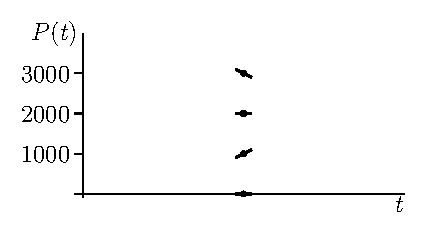
\includegraphics{pop1}
\end{center}
\end{efig}
As a result,
\begin{itemize}
  \item  if $P(0)=0$, the graph starts out horizontally. In other
    words, as $t$ starts to increase, $P(t)$ remains at zero, so the slope
    of the graph remains at zero. The population
    size remains zero for all time. As a check, observe that
    the function $P(t)=0$ obeys $\diff{P}{t}(t)=\big(6000-3P(t)\big)P(t)$
    for all $t$.

  \item  Similarly, if $P(0)=2000$, the graph again starts out
    horizontally. So $P(t)$ remains at $2000$ and the slope remains at zero.
    The population size remains 2000 for all time. Again, the function
    $P(t)=2000$ obeys $\diff{P}{t}(t)=\big(6000-3P(t)\big)P(t)$ for all $t$.

  \item  If $P(0)=1000$, the graph starts out with positive slope.
    So $P(t)$ increases with $t$. As $P(t)$ increases towards 2000, the slope
    $(6000-3P(t)\big)P(t)$, while remaining positive, gets closer and closer
    to zero. As the graph approaches height 2000, it becomes more and more
    horizontal. The graph cannot actually cross from below 2000 to above 2000,
    because to do so, it would have to have strictly positive slope for
    some value of $P$ above 2000, which is not allowed.
\issue{Joel:\\Mention\\uniqueness\\of solutions\\to IVP's?}

  \item  If $P(0)=3000$, the graph starts out with negative slope.
    So $P(t)$ decreases with $t$. As $P(t)$ decreases towards 2000, the slope
    $(6000-3P(t)\big)P(t)$, while remaining negative, gets closer and closer
    to zero. As the graph approaches height 2000, it becomes more and more
    horizontal. The graph cannot actually cross from above 2000 to below 2000,
    because to do so, it would have to have negative slope for some value of
    $P$ below 2000. which is not allowed.
\end{itemize}

\noindent These curves are sketched in the figure below. We conclude that
for any initial population size $P(0)$, except $P(0)=0$, the population
size approaches $2000$ as $t\rightarrow\infty$.

\begin{fig}
\begin{center}
   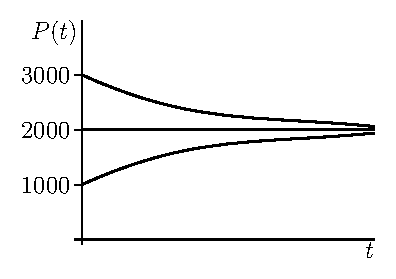
\includegraphics{pop2}
\end{center}
\end{fig}

\begin{comment}




%%%%%%%%%%%%%%%%%%%%%%%%%%%%%%%%%%%%%%%%%%%%%%%%%%%%%%%%%%%%%%%%%
\subsection{Interest on Investments}\label{sec:APPinterest}
%%%%%%%%%%%%%%%%%%%%%%%%%%%%%%%%%%%%%%%%%%%%%%%%%%%%%%%%%%%%%%%%%

Suppose that you deposit $\$P$ in a bank account at time $t=0$.
The account pays $r\%$ interest per year compounded $n$ times per year.

\begin{itemize} \itemsep1pt \parskip0pt
  \item  The first interest payment is made at time $t=\frac{1}{n}$.
         Because the balance in the account during the time interval
         $0<t<\frac{1}{n}$ is $\$P$ and interest is being paid for
         $\big(\frac{1}{n}\big)^\mathrm{th}$ of a year, that first
         interest payment is $\frac{1}{n}\times\frac{r}{100}\times P$.
         After the first interest payment, the balance in the account is
         $P+\frac{1}{n}\times\frac{r}{100}\times P
          =  \big(1+\frac{r}{100n}\big)P$.
  \item  The second interest payment is made at time $t=\frac{2}{n}$.
         Because the balance in the account during the time interval
         $\frac{1}{n}<t<\frac{2}{n}$ is $\big(1+\frac{r}{100n}\big)P$
         and interest is being paid for $\big(\frac{1}{n}\big)^\mathrm{th}$
         of a year, the second  interest payment is
          $\frac{1}{n}\times\frac{r}{100}\times \big(1+\frac{r}{100n}\big)P$.
         After the second interest payment, the balance in the account is
\begin{align*}
\big(1+\frac{r}{100n}\big)P+\frac{1}{n}\times\frac{r}{100}\times
         \big(1+\frac{r}{100n}\big)P
          &=  \big(1+\frac{r}{100n}\big)^2P
\end{align*}
  \item  And so on.
\end{itemize}
In general, at time $t=\frac{m}{n}$ (just after the $m^\mathrm{th}$ interest
payment), the balance in the account is
\begin{equation}\label{eq:APPdiscreteCompounding}
         B(t) = \Big(1+\frac{r}{100n}\Big)^m P
              = \Big(1+\frac{r}{100n}\Big)^{nt}P
\end{equation}
Three common values of $n$ are $1$ (interest is paid once a year),
$12$ (i.e. interest is paid once a month) and 365 (i.e. interest is paid
daily).
The limit $n\rightarrow\infty$ is called continuous compounding\footnote{There
are banks that advertise continuous compounding. You can find some by googling
``interest is compounded continuously and paid''}. Under continuous compounding,
the balance at time $t$ is
\begin{align*}
B(t) &= \lim_{n\rightarrow\infty} \Big(1+\frac{r}{100n}\Big)^{nt}P \\
\end{align*}
Let's call $\frac{r}{100n}=x$. As $n\rightarrow \infty$, $x\rightarrow 0$
and the exponent $nt = \frac{r}{100x}t$ tends to infinity. In
Example~\ref{eg:moneyA} below, we show that
\begin{align*}
B(t) &= e^{rt/100} P.
\end{align*}
%
%
% We saw, in
% Example \ref{clp_diff-eg:bigohlimitA}, that
% \begin{align*}
% \lim_{x\rightarrow 0}(1+x)^{a/x}=e^a
% \end{align*}
% Writing $x=\frac{r}{100n}$ and $a=\frac{rt}{100}$ (so that $nt=\frac{a}{x}$),
% we have
% \begin{equation}\label{eq:APPcontinuousCompounding}
% B(t) = \lim_{n\rightarrow\infty} \Big(1+\frac{r}{100n}\Big)^{nt}P
%      =\lim_{x\rightarrow 0}(1+x)^{a/x}P=e^aP
%      = e^{rt/100}P
% \end{equation}

%%%%%%%%%%%%%%%%%%%%%%%%%
\begin{eg}\label{eg:moneyA}
In this example we'll derive the formula
\begin{align*}
  B(t) &= e^{rt/100} P.
\end{align*}
using a differential equation.

Again, suppose that you deposit $\$P$ in a bank account at time $t=0$, and that
the
account pays $r\%$ interest per year
compounded $n$ times per year, and denote by $B(t)$ the balance at time
$t$. Suppose that you have just received an interest payment at time $t$.
Then the next interest payment will be made at time $t+\frac{1}{n}$
and will be $\frac{1}{n}\times\frac{r}{100}\times B(t)=\frac{r}{100n}B(t)$.
So, calling $\frac{1}{n}=h$,
\begin{align*}
B(t+h)=B(t) + \frac{r}{100}B(t)h\qquad\text{or}\qquad
\frac{B(t+h)-B(t)}{h} = \frac{r}{100}B(t)
\end{align*}
To get continuous compounding we take the limit $n\rightarrow\infty$,
or equivalently $h\rightarrow 0$. This gives
\begin{align*}
\lim_{h\rightarrow 0}\frac{B(t+h)-B(t)}{h} = \frac{r}{100}B(t)
\qquad\text{or}\qquad
\diff{B}{t}(t) = \frac{r}{100}B(t)
\end{align*}
By Theorem \ref{thm:growthDEsoln}, $B(t)$ obeys this differential equation
if and only if there is a constant $C$ such that $B(t)=Ce^{rt/100}$.
Since $C=B(0)=P$, we have $B(t)=e^{rt/100}P$.
\end{eg}
\goodbreak
%%%%%%%%%%%%%%%%%%%%%%%%%
\begin{eg}\label{eg:moneyB}
\begin{enumerate}[(a)]
\item A bank advertises that it compounds interest continuously and that
it will double your money in ten years. What is the annual interest rate?

\item A bank advertises that it compounds monthly and that it will
double your money in ten years. What is the annual interest rate?
\end{enumerate}

\soln (a)
Let the interest rate be $r\%$ per year. If you start with $\$P$, then
after $t$ years, you have $Pe^{rt/100}$, under continuous compounding.
This was \eqref{eq:APPcontinuousCompounding}.
After 10 years you have $Pe^{r/10}$. This is supposed to be $2P$, so
$$
Pe^{r/10}=2P\quad\Longrightarrow\quad
e^{r/10}=2\quad\Longrightarrow\quad
\frac{r}{10}=\log 2\quad\Longrightarrow\quad
r=10\log2 =6.93\%
$$


\noindent (b)
Let the interest rate be $r\%$ per year. If you start with $\$P$, then
after $t$ years, you have $P\big(1+\frac{r}{100\times 12}\big)^{12 t}$,
under monthly compounding. This was \eqref{eq:APPdiscreteCompounding}.
After 10 years you have $P\big(1+\frac{r}{100\times 12}\big)^{120}$. This is
supposed to
be $2P$, so
\begin{align*}
&P\big(1+\frac{r}{100\times 12}\big)^{120}=2P
&&\Longrightarrow\quad
    \big(1+\frac{r}{1200}\big)^{120}=2\quad\Longrightarrow\quad
1+\frac{r}{1200}=2^{1/120}\\
&\Longrightarrow\quad \frac{r}{1200}=2^{1/120}-1
&&\Longrightarrow\quad
r=1200\big(2^{1/120}-1\big) =6.95\%
\end{align*}



\end{eg}
%%%%%%%%%%%%%%%%%%%%%%%%%
\begin{eg}\label{eg:moneyC}
A 25 year old graduate of UBC is given \$50,000 which is invested
at 5\% per year compounded continuously. The graduate also intends to
deposit money continuously at the rate of \$2000 per year. Assuming that
the interest rate remains 5\%, the amount $A(t)$ of money at time $t$ satisfies
the equation
$$
\diff{A}{t}= 0.05 A+2000
$$
\begin{enumerate}[(a)]
\item  Determine the amount of money in the account when the graduate
is 65.
\item  At age 65, the graduate will withdraw money continuously
at the rate of $W$ dollars per year. If the money must last until the person
is 85, what is the largest possible value of $W$?
\end{enumerate}

\soln (a) The amount of money at time $t$ obeys
\begin{align*}
\diff{A}{t}= 0.05 A(t)+2,\!000=0.05\big(A(t)+40,\!000\big)
\end{align*}
So by Corollary \ref{cor:coolingDEsoln},
(with $K=0.05$ and the $A$ of Corollary \ref{cor:coolingDEsoln}
being $-40,\!000$)
\begin{align*}
A(t)=-40,\!000+\big(A(0)+40,\!000\big)e^{0.05 t}
\end{align*}
At time 0 (when the graduate is 25), $A(0)=50,\!000$, so the amount of
money at time $t$ is
\begin{align*}
A(t)=90,\!000\, e^{0.05 t}-40,000
\end{align*}
In particular, when the graduate is 65 years old, $t=40$ and
\begin{align*}
A(40)=90,\!000\, e^{0.05 \times 40}-40,000=\text{\$625,015.05 }
\end{align*}

\noindent(b) When the graduate stops depositing money and instead
starts withdrawing money at a rate $W$, the equation for $A$ becomes
\begin{align*}
\diff{A}{t}= 0.05 A-W= 0.05 (A-20 W)
\end{align*}
assuming that the interest rate remains 5\%.
Thus time, Corollary \ref{cor:coolingDEsoln},
(with $K=0.05$ and the $A$ of Corollary \ref{cor:coolingDEsoln} being $20W$)
gives
\begin{align*}
A(t)=20W+\big(A(0)-20W\big)e^{0.05 t}
\end{align*}
If we now reset our clock so that $t=0$ when the graduate is 65,
$A(0)=625,015.05$. So the amount of money at time $t$ is
\begin{align*}
A(t)=20W+ e^{0.05 t}(625,015.05-20W)
\end{align*}
We want the account to be depleted when the graduate is 85. So, we
want $A(20)=0$. This is the case if
\begin{align*}
20W+ e^{0.05\times 20}(625,015.05-20W)=0
&\implies
20W+ e(625,015.05-20W)=0\\
&\implies
20(e-1)W= 625,015.05e\\
&\implies
W=\frac{625,015.05e}{20(e-1)}=\$49,437.96
\end{align*}
\end{eg}







%%%%%%%%%%%%%%%%%%%%%%%%%%%%%%%%%%%%%%%%%%%%%%%%%%%%%%%%%%%%%%%%%
\subsection{Terminal Velocity}\label{ssec term vel}
%%%%%%%%%%%%%%%%%%%%%%%%%%%%%%%%%%%%%%%%%%%%%%%%%%%%%%%%%%%%%%%%%

\begin{eg}\label{eg:terminalVelocity}
We now return to the differential equation \eqref{eq:linearAirResistance}.
The unknown function $v(t)$ in that equation is the velocity of a
falling body. With a little trickery, we can convert the differential
equation \eqref{eq:linearAirResistance} into the differential
equation \eqref{eq:carbonDating}. This will give us the general
solution to \eqref{eq:linearAirResistance}. All we have to do is rewrite
\eqref{eq:linearAirResistance} as
\begin{align*}
\diff{v}{t}(t) = g -\frac{\beta}{m} v(t)
               = -\frac{\beta}{m}\Big[ v(t) -\frac{mg}{\beta}\Big]
\end{align*}
Since the derivative of any constant is zero, this is equivalent to
\begin{equation}\label{eq:linearAirResistanceB}
\diff{}{t}\Big[ v(t) -\frac{mg}{\beta}\Big]
               = -\frac{\beta}{m}\Big[ v(t) -\frac{mg}{\beta}\Big]
\end{equation}
The point here is that \eqref{eq:linearAirResistanceB} is exactly
\eqref{eq:carbonDating}, i.e. $\diff{}{t} Q(t)=-kQ(t)$, with
$Q(t)= \big[ v(t) -\frac{mg}{\beta}\big] $ and $k=\frac{\beta}{m}$.
So $v(t)$ is a solution to \eqref{eq:linearAirResistance} if and only if
there is a constant $C$ such that
\begin{align*}
Q(t)= \big[ v(t) -\frac{mg}{\beta}\big] = Ce^{-kt} = Ce^{-\frac{\beta}{m} t}
\iff v(t) = Ce^{-\frac{\beta}{m} t} +\frac{mg}{\beta}
\end{align*}


Let's see what this tells us about the velocity of our falling body. Suppose
that the body was dropped, from rest, at time $0$. That is, at time $t=0$,
we have $v(0)=0$ and
\begin{align*}
0=v(0) = C +\frac{mg}{\beta}
\end{align*}
 This tell us that our constant $C=-\frac{mg}{\beta}$ and that our velocity
at time $t$ is
\begin{align*}
v(t) = \frac{mg}{\beta}\Big[1-e^{-\frac{\beta}{m} t}\Big]
\end{align*}
So
\begin{itemize} \itemsep1pt \parskip0pt
  \item  At $t=0$, $e^{-\frac{\beta}{m} t}=e^{-\frac{\beta}{m} 0}=1$
         and the velocity is
          $v(0)%=\frac{mg}{\beta}\big[1-e^{-\frac{\beta}{m} 0}\big]
                =\frac{mg}{\beta}\big[1-1\big]=0$.
           (Just checking --- we already knew this.)
  \item  As $t$ increases, $e^{-\frac{\beta}{m} t}$ decreases
               so that $1-e^{-\frac{\beta}{m} t}$ increases. Thus, as $t$
               increases the velocity $v(t)$ increases. That makes sense.
  \item  But as $t$ tends to $\infty$, $e^{-\frac{\beta}{m} t}$ tends to zero,
               so that $1-e^{-\frac{\beta}{m} t}$ tends to one and
               $v(t)$ tends to $\frac{mg}{\beta}$. The velocity approaches,
               but never actually achieves, let alone surpasses,
               $\frac{mg}{\beta}$. This limiting velocity,
               $\frac{mg}{\beta}$ is called the terminal velocity.
\end{itemize}
Here is a sketch of the graph of $v(t)$.
\begin{efig}
\begin{center}
    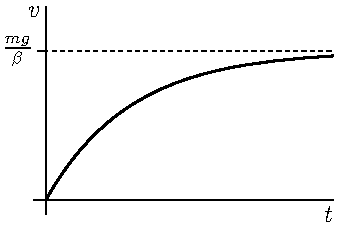
\includegraphics{terminalVelocity}
\end{center}
\end{efig}
\end{eg}


\begin{eg}\label{eg:eg:elephantMouse}
  Assume that an object of mass $m$ falling near the surface of
the earth is retarded by air resistance that is proportional to its speed
and to its cross--sectional area\footnote{The bigger the cross--sectional
area, the greater the number of impacts between atmospheric molecules
and the object, and consequently, the greater the air resistance.},
with the latter proportional\footnote{To motivate this, let's assume
that the object is a sphere of radius $r$ and density $\rho$. Then the
object has mass $m = \frac{4}{3}\pi r^3 \rho$ and its cross--sectional
area is $\pi r^2$, which is a constant times
$m^{2/3}=\big(\frac{4}{3}\pi\rho\big)^{2/3}r^2$.} to
$(\text{mass})^{2/3}$, so that, by Newton's law of motion,
$$
m\diff{v}{t}=mg-km^{2/3}v
$$
where $v=v(t)$ is the speed of the object at time $t$ and $g$ is the
acceleration of gravity.

\begin{enumerate}[(a)]
\item  Which has a higher terminal velocity,  a mouse or an elephant?
\item
Which reaches half its terminal velocity first, when dropped from rest?
\end{enumerate}

\soln
We have seen, in Example \ref{eg:terminalVelocity} with
$\beta=km^{2/3}$, that
\begin{equation*}
v(t) = \frac{mg}{\beta}\Big[1-e^{-\frac{\beta}{m} t}\Big]
= \frac{gm^{1/3}}{k}\Big[1-e^{-\frac{k}{m^{1/3}} t}\Big]
\end{equation*}

\noindent(a) Since $\lim\limits_{t\rightarrow\infty}e^{-km^{-1/3}t}=0$,
the terminal velocity, $\lim\limits_{t\rightarrow\infty}v(t)$, is
$\frac{gm^{1/3}}{k}$, which is \emph{larger for an elephant}.


\noindent(b)  One half of this terminal velocity is reached
when $e^{-km^{-1/3}t}=\half$. This happens at
$t=\frac{m^{1/3}}{k}\log 2$, which is \emph{sooner for a mouse}.


\end{eg}
\end{comment}

\graphicspath{{figures/differentiation/}}

%%%%%%%%%%%%%%%%%%%%%%%%%%%%%%%%%%%%%%%%%%%%%%
\longsection{Approximating Functions Near a Specified Point
--- Taylor Polynomials}{Taylor polynomials}\label{sec:DIFFTaylor}
%%%%%%%%%%%%%%%%%%%%%%%%%%%%%%%%%%%%%%%%%%%%%
Suppose that you are interested in the values of some function $f(x)$ for
$x$ near some fixed point $a$. When the function is a polynomial or a rational
function we can use some arithmetic (and maybe some hard work) to write down
the answer. For example:
\begin{align*}
  f(x) &= \frac{x^2-3}{x^2-2x+4} \\
  f(1/5) &= \frac{ \frac{1}{25}-3}{\frac{1}{25}-\frac{2}{5}+4 }
  = \frac{\frac{1-75}{25} }{\frac{1-10+100}{25}}\\
  &= \frac{-74}{91}
\end{align*}
Tedious, but we can do it. On the other hand if you are asked to compute
$\sin(1/10)$ then what can we do? We know that a calculator can work it out
\begin{align*}
  \sin(1/10) &= 0.09983341\dots
\end{align*}
but how does the calculator do this? How did people compute this before
calculators\footnote{Originally the word ``calculator'' referred not to the
software or electronic (or even mechanical) device we think of today, but
rather to a person who performed calculations.}? A hint comes from the
following sketch of $\sin(x)$ for $x$ around $0$.

\begin{fig}
 \begin{center}
  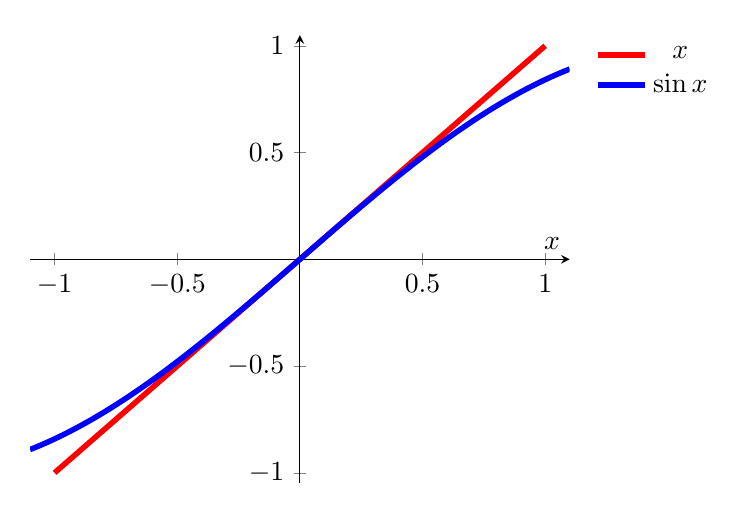
\begin{tikzpicture}
  \begin{axis}[
  axis x line=center, axis y line=center,
  ymax=1.05,ymin=-1.05, ytick={-1,-0.5,0.5,1.0},
  xtick={-1,-0.5,0.5,1},
  xlabel=$x$,
  legend entries={$x$,$\sin x$},
  legend pos=outer north east,
  legend style={draw=none}
  ]
  \addplot[line width=2pt, red,domain=-1:1,samples=100] {x};
  \addplot[line width=2pt, blue,domain=-1.1:1.1,samples=100] {sin(deg(x))};
  \end{axis}
\end{tikzpicture}
 \end{center}
\end{fig}
The above figure shows that the curves $y=x$ and $y=\sin x$ are almost the same
when $x$ is close to $0$. Hence if we want the value of
$\sin(1/10)$ we could just use this approximation $y=x$ to get
\begin{align*}
  \sin(1/10) \approx 1/10.
\end{align*}
Of course, in this case we simply observed that one function was a good
approximation of the other. We need to know how to find such approximations
more systematically.

More precisely, say we are given a function $f(x)$ that we wish to approximate
close to some point $x=a$, and we need to find another function $F(x)$
that
\begin{itemize}
 \item is simple and easy to compute\footnote{It is no good approximating a
function with something that is even more difficult to work with.}
 \item is a good approximation to $f(x)$ for $x$ values close to $a$.
\end{itemize}
Further, we would like to understand how good our approximation actually is.
Namely we need to be able to estimate the error $|f(x)-F(x)|$.

There are many different ways to approximate a function and we will discuss one
family of approximations: Taylor polynomials. This is an infinite family of
ever improving approximations, and our starting point is the very simplest.


%%%%%%%%%%%%%%%%%%%%%%%%%%%%%%%%%%%%%%%%%%%%%%%%%%%%%%%%%%%%%%%%%%%%%%
\subsection{Zeroth Approximation --- the Constant Approximation}\label{ssec const approx}
%%%%%%%%%%%%%%%%%%%%%%%%%%%%%%%%%%%%%%%%%%%%%%%%%%%%%%%%%%%%%%%%%%%%%%
The simplest functions are those that are constants. And our
zeroth\footnote{It barely counts as an approximation at all, but it will help
build intuition. Because of this, and the fact that a constant is a
polynomial of degree 0,  we'll start counting our approximations from zero
rather than 1.} approximation will be by a constant function. That is, the
approximating function will have the form $F(x)=A$, for some constant $A$.
Notice that this function is a polynomial of degree zero.


To ensure that $F(x)$ is a good approximation for $x$ close to $a$, we choose
$A$ so that $f(x)$ and $F(x)$ take exactly the same value when $x=a$.
\begin{align*}
F(x)=A\qquad\text{so}\qquad F(a)=A=f(a)\implies A=f(a)
\end{align*}
Our first, and crudest, approximation rule is
\begin{impeqn}[Constant approximation]\label{eq:constApprox}
\begin{align*}
f(x)\approx f(a)
\end{align*}
\end{impeqn}
\noindent An important point to note is that we need to know $f(a)$ --- if we cannot
compute that easily then we are not going to be able to proceed. We will often
have to choose $a$ (the point around which we are approximating $f(x)$) with
some care to ensure that we can compute $f(a)$.


Here is a figure showing the graphs of a typical $f(x)$ and approximating
function $F(x)$.
\vadjust{
    \begin{efig}
    \begin{center}
       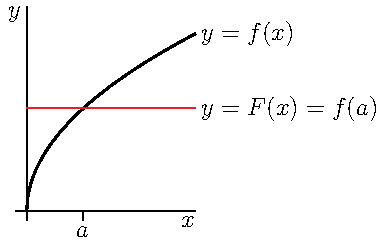
\includegraphics{approx1}
    \end{center}
    \end{efig}
}
At $x=a$, $f(x)$ and $F(x)$ take the same value. For $x$ very near $a$,
the values of $f(x)$ and $F(x)$ remain close together. But the quality
of the approximation deteriorates fairly quickly as $x$ moves
away from $a$. Clearly we could do better with a straight line that follows the slope of
the curve. That is our next approximation.

But before then, an example:
\begin{eg}\label{eg ex const approx}
 Use the constant approximation to estimate $e^{0.1}$.

\soln First set $f(x) = e^x$.
\begin{itemize}
 \item Now we first need to pick a point $x=a$  to approximate the function. This point
needs to be close to $0.1$ and we need to be able to evaluate $f(a)$ easily. The obvious
choice is $a=0$.
\item Then our constant approximation is just
\begin{align*}
  F(x) &= f(0) = e^0 = 1\\
  F(0.1) &= 1
\end{align*}
\end{itemize}
Note that $e^{0.1} = 1.105170918\dots$, so even this approximation isn't too bad..
\end{eg}






%%%%%%%%%%%%%%%%%%%%%%%%%%%%%%%%%%%%%%%%%%%%%%%%%%%%%%%%%%%%%%%%%%%%%%
\subsection{First Approximation --- the Linear approximation}
%%%%%%%%%%%%%%%%%%%%%%%%%%%%%%%%%%%%%%%%%%%%%%%%%%%%%%%%%%%%%%%%%%%%%%
Our first\footnote{Recall that we started counting from
zero.} approximation improves on our zeroth approximation by allowing the approximating
function to be a linear function of $x$ rather than just a constant function. That is, we
allow $F(x)$ to be of the form $A+Bx$, for some constants $A$ and $B$.


To ensure that $F(x)$ is a good approximation for $x$ close to $a$, we still require that
$f(x)$ and $F(x)$ have the same value at $x=a$ (that was our zeroth approximation). Our
additional requirement is that their tangent lines at $x=a$ have the same slope --- that
the derivatives of $f(x)$ and $F(x)$ are the same at $x=a$. Hence
\begin{align*}
F(x)&=A+Bx  & &\implies & F(a)=A+Ba&=f(a)\\
F'(x)&=B    & &\implies & F'(a)=\phantom{A+a}B&=f'(a)
\end{align*}
So we must have $B=f'(a)$. Substituting this into $A+Ba=f(a)$ we get
$A=f(a)-af'(a)$. So
we can write
\begin{align*}
  F(x) &= A+Bx = \overbrace{f(a)- af'(a)}^A+ f'(a) \cdot x \\
  &= f(a) + f'(a) \cdot(x-a)
\end{align*}
We write it in this form because we can now clearly see that our first approximation is
just an extension of our zeroth approximation. This first approximation is also often
called the linear approximation of $f(x)$ about $x=a$.
\begin{impeqn}[Linear approximation]\label{eq:linApprox}
\begin{align*}
  f(x) \approx f(a)+f'(a)(x-a)
\end{align*}
\end{impeqn}
\noindent We should again stress that in order to form this approximation we need to know
$f(a)$ and $f'(a)$ --- if we cannot compute them easily then we are not going to be able
to proceed.



Recall, from Theorem \ref{thm:DIFFtangentLine}, that $y=f(a)+f'(a)(x-a)$
is exactly the equation of the tangent line to the curve $y=f(x)$ at $a$.
Here is a figure showing the graphs of a typical $f(x)$ and the approximating
function $F(x)$.
\vadjust{
    \begin{efig}
    \begin{center}
       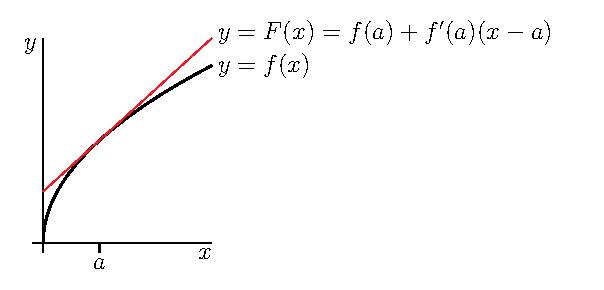
\includegraphics{approx2}
    \end{center}
    \end{efig}
}
Observe that the graph of $f(a)+f'(a)(x-a)$ remains close to the
graph of $f(x)$ for a much larger range of $x$ than did the graph of our constant
approximation, $f(a)$. One can also see that we can improve this approximation if we can
use a function that curves down rather than being perfectly straight. That is our next
approximation.

But before then, back to our example:
\begin{eg}
 Use the linear approximation to estimate $e^{0.1}$.

\soln First set $f(x) = e^x$ and $a=0$ as before.
\begin{itemize}
 \item To form the linear approximation we need $f(a)$ and $f'(a)$:
\begin{align*}
  f(x) &= e^x & f(0) & = 1 \\
  f'(x) &= e^x & f'(0) & = 1
\end{align*}
\item Then our linear approximation is
\begin{align*}
  F(x) &= f(0) + x f'(0) = 1 + x \\
  F(0.1) &= 1.1
\end{align*}
\end{itemize}
Recall that $e^{0.1} = 1.105170918\dots$, so the linear approximation is
almost correct to 3 digits.
\end{eg}

It is worth doing another simple example here.
\begin{eg}
 Use a linear approximation to estimate $\sqrt{4.1}$.

\soln First set $f(x)=\sqrt{x}$. Hence $f'(x) = \frac{1}{2\sqrt{x}}$. Then we are trying
to approximate $f(4.1)$. Now we need to choose a sensible $a$ value.
\begin{itemize}
 \item We need to choose $a$ so that $f(a)$ and $f'(a)$ are easy to compute.
\begin{itemize}
 \item We could try $a=4.1$ --- but then we need to compute $f(4.1)$ and $f'(4.1)$ ---
which is our original problem and more!
\item We could try $a=0$ --- then $f(0)=0$ and $f'(0) = DNE$.
\item Setting $a=1$ gives us $f(1)=1$ and $f'(1)=\frac{1}{2}$. This would work, but we
can get a better approximation by choosing $a$ is closer to $4.1$.
\item Indeed we can set $a$ to be the square of any rational number and we'll get a
result that is easy to compute.
\item Setting $a=4$ gives $f(4)=2$ and $f'(4) = \frac{1}{4}$. This seems good enough.
\end{itemize}
\item Substitute this into equation~\eqref{eq:linApprox} to get
\begin{align*}
  f(4.1) &\approx f(4) + f'(4) \cdot(4.1-4) \\
  &= 2 + \frac{0.1}{4} = 2 + 0.025 = 2.025
\end{align*}
\end{itemize}
Notice that the true value is $\sqrt{4.1} = 2.024845673\dots$.
\end{eg}



%%%%%%%%%%%%%%%%%%%%%%%%%%%%%%%%%%%%%%%%%%%%%%%%%%%%%%%%%%%%%%%%%%%%%%
\subsection{Second Approximation --- the Quadratic Approximation}
%%%%%%%%%%%%%%%%%%%%%%%%%%%%%%%%%%%%%%%%%%%%%%%%%%%%%%%%%%%%%%%%%%%%%%

We next develop a still better approximation by now allowing the
approximating function be to a quadratic function of $x$. That is,
we allow $F(x)$ to be of the form $A+Bx+Cx^2$, for some constants $A$, $B$
and $C$. To ensure that $F(x)$ is a good approximation for $x$ close
to $a$, we choose $A$, $B$ and $C$ so that
\begin{itemize}
  \item $f(a)=F(a)$  (just as in our zeroth approximation),
  \item $f'(a)=F'(a)$ (just as in our first approximation), and
  \item $f''(a)=F''(a)$ --- this is a new condition.
\end{itemize}
These conditions give us the following equations
\begin{align*}
F(x)&=A+Bx+Cx^2  & &\implies & F(a)=A+Ba+\phantom{2}Ca^2&=f(a)\\
F'(x)&=B+2Cx & &\implies & F'(a)=\phantom{A+a}B+2Ca&=f'(a)\\
F''(x)&=2C   & &\implies & F''(a)=\phantom{A+aB+a}2C&=f''(a)
\end{align*}
Solve these for $C$ first, then $B$ and finally $A$.
\begin{align*}
C &=\half f''(a) & \text{substitute}\\
B &= f'(a) - 2Ca = f'(a)-af''(a) & \text{substitute again}\\
A &= f(a)-Ba-Ca^2 = f(a)-a[f'(a)-af''(a)]-\half f''(a)a^2
\end{align*}
Then put things back together to build up $F(x)$:
\begin{align*}
F(x)&=f(a)-f'(a)a+\half f''(a)a^2 & &\text{(this line is $A$)}\cr
&\phantom{=f(a)\hskip3pt}+f'(a)\,x\hskip3pt- f''(a)ax
   & & \text{(this line is $Bx$)}\\
&\phantom{=f(a)-f'(a)a\hskip3.5pt}+\half f''(a)x^2
 & &\text{(this line is $Cx^2$)}\\
&=f(a)+f'(a)(x-a)+\half f''(a)(x-a)^2
\end{align*}
Oof! We again write it in this form because we can now clearly see that our second
approximation is just an extension of our first approximation.

Our second approximation is called the quadratic approximation:
\begin{impeqn}[Quadratic approximation]\label{eq:quadApprox}
\begin{align*}
f(x)\approx f(a)+f'(a)(x-a)+\half f''(a)(x-a)^2
\end{align*}
\end{impeqn}
\noindent Here is a figure showing the graphs
of a typical $f(x)$ and approximating function $F(x)$.
\vadjust{
    \begin{efig}
    \begin{center}
       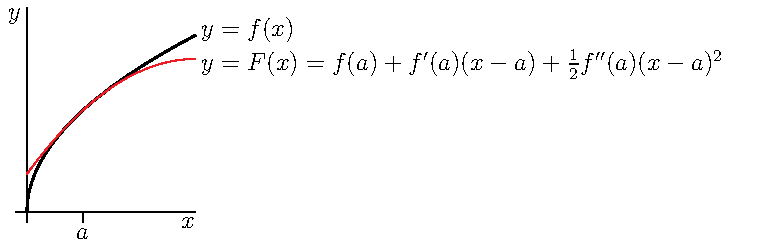
\includegraphics{approx3}
    \end{center}
    \end{efig}
}
This new approximation looks better than both the first and second.


Now there is actually an easier way to derive this approximation, which we show
you now. Let us rewrite\footnote{Any polynomial of degree two can be written in
this form. For example, when $a=1$, $3 + 2x + x^2 =   6 +  4(x-1) + (x-1)^2$.}
$F(x)$ so that it is easy to evaluate it and its derivatives at $x=a$:
\begin{align*}
  F(x) &= \alpha + \beta\cdot (x-a) + \gamma \cdot(x-a)^2
\end{align*}
Then
\begin{align*}
  F(x) &= \alpha + \beta\cdot (x-a) + \gamma \cdot(x-a)^2 &
  F(a) &= \alpha = f(a) \\
  F'(x) &= \beta + 2\gamma \cdot(x-a) &
  F'(a)&=\beta = f'(a) \\
  F''(x) &= 2\gamma &
  F''(a) &= 2\gamma = f''(a)
\end{align*}
And from these we can clearly read off the values of $\alpha,\beta$ and $\gamma$ and so
recover our function $F(x)$. Additionally if we write things this way, then it is quite
clear how to extend this to a cubic approximation and a quartic approximation and so
on.

Return to our example:
\begin{eg}
 Use the quadratic approximation to estimate $e^{0.1}$.

\soln Set $f(x) = e^x$ and $a=0$ as before.
\begin{itemize}
 \item To form the quadratic approximation we need $f(a), f'(a)$ and $f''(a)$:
\begin{align*}
  f(x) &= e^x & f(0) & = 1 \\
  f'(x) &= e^x & f'(0) & = 1\\
  f''(x) &= e^x & f''(0) & = 1
\end{align*}
\item Then our quadratic approximation is
\begin{align*}
  F(x) &= f(0) + x f'(0)  + \frac{1}{2} x^2 f''(0) = 1 + x + \frac{x^2}{2} \\
  F(0.1) &= 1.105
\end{align*}
\end{itemize}
Recall that $e^{0.1} = 1.105170918\dots$, so the quadratic approximation is quite
accurate with very little effort.
\end{eg}



Before we go on, let us first introduce (or revise) some notation that will make our
discussion easier.




%%%%%%%%%%%%%%%%%%%%%%%%%%%%%%%%%%%%%%%%%%%%%%%%%%%%%%%%%%%%%%%%%%%%%%

\subsection*{Whirlwind Tour of Summation Notation}
In the remainder of this section we will frequently need to write sums involving a
large number of terms. Writing out the summands explicitly can become quite
impractical --- for example, say we need the sum of the first 11 squares:
\begin{align*}
  1 + 2^2 + 3^2 + 4^2+ 5^2 + 6^2 + 7^2 + 8^2 + 9^2 + 10^2 + 11^2
\end{align*}
This becomes tedious. Where the pattern is clear, we will often skip the middle few
terms and instead write
\begin{align*}
  1 + 2^2 + \cdots  + 11^2.
\end{align*}
A far more precise way to write this is using $\Sigma$ (capital-sigma) notation. For
example, we can write the above sum as
\begin{align*}
  \sum_{k=1}^{11} k^2
\end{align*}
This is read as
\begin{quote}
 The sum from $k$ equals 1 to 11 of $k^2$.
\end{quote}
More generally
\begin{notn}
Let $m\leq n$ be integers and let $f(x)$ be a function defined on the integers.
Then we write
\begin{align*}
  \sum_{k=m}^n f(k)
\end{align*}
to mean the sum of $f(k)$ for $k$ from $m$ to $n$:
\begin{align*}
  f(m) + f(m+1) + f(m+2) + \cdots + f(n-1) + f(n).
\end{align*}
Similarly we write
\begin{align*}
  \sum_{i=m}^n a_i
\end{align*}
to mean
\begin{align*}
  a_m+a_{m+1}+a_{m+2}+\cdots+a_{n-1}+a_n
\end{align*}
for some set of coefficients $\{ a_m, \ldots, a_n \}$.
\end{notn}

Consider the example
\begin{align*}
\sum_{k=3}^7 \frac{1}{k^2}=\frac{1}{3^2}+\frac{1}{4^2}+\frac{1}{5^2}+
\frac{1}{6^2}+\frac{1}{7^2}
\end{align*}
It is important to note that the right hand side of this expression evaluates to a
number\footnote{Some careful addition shows it is $\frac{46181}{176400}$.}; it does not
contain ``$k$''.  The summation index $k$  is just a ``dummy'' variable and
it does not have to be called $k$. For example
\begin{align*}
  \sum_{k=3}^7 \frac{1}{k^2}
  =\sum_{i=3}^7 \frac{1}{i^2}
  =\sum_{j=3}^7 \frac{1}{j^2}
  =\sum_{\ell=3}^7 \frac{1}{\ell^2}
\end{align*}
Also the summation index has no meaning outside the sum. For
example
\begin{align*}
k\sum_{k=3}^7 \frac{1}{k^2}
\end{align*}
has no mathematical meaning; It is gibberish\footnote{Or possibly gobbledygook. For a
discussion of statements without meaning and why one should avoid them we recommend the
book ``Bendable learnings: the wisdom of modern management'' by Don Watson.}.



%%%%%%%%%%%%%%%%%%%%%%%%%%%%%%%%%%%%%%%%%%%%%%%%%%%%%%%%%%%%%%%%%%%%%%
\subsection{Still Better Approximations --- Taylor Polynomials}
%%%%%%%%%%%%%%%%%%%%%%%%%%%%%%%%%%%%%%%%%%%%%%%%%%%%%%%%%%%%%%%%%%%%%%
We can use the same strategy to generate still better approximations by
polynomials\footnote{Polynomials are generally a good choice for an approximating
function since they are so easy to work with. Depending on the situation other families
of functions may be more appropriate. For example if you are approximating a periodic
function, then sums of sines and cosines might be a better choice; this leads to Fourier
series.} of any degree we like. As was the case with the approximations above, we
determine the coefficients of the polynomial by requiring, that at the point
$x=a$, the approximation and its first $n$ derivatives agree with those of the
original function.

Rather than simply moving to a cubic polynomial, let us try to write things in a more
general way. We will consider approximating the function $f(x)$ using a polynomial,
$T_n(x)$, of degree $n$ --- where $n$ is a non-negative integer. As we discussed
above, the algebra is easier if we write
\begin{align*}
  T_n(x) &= c_0 + c_1(x-a) + c_2 (x-a)^2 + \cdots + c_n (x-a)^n\\
  &= \sum_{k=0}^n c_k (x-a)^k & \text{using $\Sigma$
notation}
\end{align*}
The above form\footnote{Any polynomial in $x$ of degree $n$ can also be
expressed as a polynomial in $(x-a)$ of the same degree $n$ and vice versa.  So
$T_n(x)$ really still is a polynomial of degree $n$.} \footnote{Furthermore
when $x$ is close to $a$, $(x-a)^k$ decreases very quickly as $k$ increases,
which often makes the "high $k$" terms in $T_n(x)$ very small. This can be a
considerable advantage when building up approximations by adding more and more
terms.  If we were to rewrite  $T_n(x)$ in the form $\ds \sum_{k=0}^n b_k x^k$
the "high $k$" terms would typically not be very small when $x$ is close to
$a$. } makes it very easy to evaluate this polynomial and its derivatives at
$x=a$. Before we proceed, we remind the reader of some notation (see
Notation~\ref{notn higher diff}):
\begin{itemize}
 \item Let $f(x)$ be a function and $k$ be a positive integer. We can denote
its $k^\mathrm{th}$ derivative with respect to $x$ by
\begin{align*}
  \ddiff{k}{f}{x} && \left( \diff{}{x}\right)^k f(x) && f^{(k)}(x)
\end{align*}
\end{itemize}

Additionally we will need
\begin{defn}[Factorial]
  Let $n$ be a positive integer\footnote{It is actually possible to define the
factorial of positive real numbers and even negative numbers but it requires more
advanced calculus and is outside the scope of this course. The interested reader should
look up the Gamma function.}, then $n$-factorial, denoted $n!$, is the product
  \begin{align*}
    n! &= n \times (n-1) \times \cdots \times 3 \times 2 \times 1
  \end{align*}
  Further, we use the convention that
  \begin{align*}
  0! &= 1
  \end{align*}
  The first few factorials are
\begin{align*}
  1! &=1 &
  2! &=2 &
  3! &=6 \\
  4! &=24 &
  5! &=120 &
  6! &=720
\end{align*}
\end{defn}

Now consider $T_n(x)$ and its derivatives:
\begin{align*}
\begin{array}{rclrrrcl}
  T_n(x) &=& c_0 &+ c_1(x-a) & + c_2 (x-a)^2 & + c_3(x-a)^3 &+ \cdots+ & c_n (x-a)^n
\\[1ex]
  T_n'(x) &=&  &c_1 & + 2 c_2 (x-a) & + 3c_3(x-a)^2 &+ \cdots +&  n c_n (x-a)^{n-1}
\\[1ex]
  T_n''(x) &=&  &  & 2 c_2 & + 6c_3(x-a) &+ \cdots +&  n(n-1) c_n (x-a)^{n-2} \\[1ex]
  T_n'''(x) &=&  &  & & 6c_3 &+ \cdots + &  n(n-1)(n-2) c_n (x-a)^{n-3} \\[1ex]
  & \vdots \\[1ex]
  T_n^{(n)}(x) &=&  &  & & & &  n! \cdot c_n
\end{array}
\end{align*}
Now notice that when we substitute $x=a$ into the above expressions only the constant
terms survive and we get
\begin{align*}
  T_n(a) &= c_0\\
  T_n'(a) &= c_1\\
  T_n''(a) &= 2\cdot c_2\\
  T_n'''(a) &= 6 \cdot c_3\\
  &\vdots \\
  T_n^{(n)}(a) &= n! \cdot c_n
\end{align*}
% We determine the coefficients $c_i$ by the requirements that $f(x)$ and
% its approximator $F(x)$ have the same value and the same first $n$
% derivatives at $x=a$.
% \begin{align*}
% F(x)&=c_0+c_1(x-a)+c_2(x-a)^2+\cdots+c_n(x-a)^n \hidewidth\\
%   &\hskip3.0in\implies  F(a)=c_0=f(a)\\
% F'(x)&=c_1+2c_2(x-a)+3c_3(x-a)^2+\cdots+nc_n(x-a)^{n-1} \hidewidth\\
%   &\hskip3.0in\implies   F'(a)=c_1=f'(a)    \displaybreak[0]\\
% F''(x)&=2c_2+3\times 2c_3(x-a)+\cdots+n(n-1)c_n(x-a)^{n-2}\hidewidth \\
%   &\hskip3.0in\implies  F''(a)=2c_2=f''(a)  \displaybreak[0]\\
% F^{(3)}(x)&=3\times 2 c_3+\cdots+n(n-1)(n-2)c_n(x-a)^{n-3} \hidewidth\\
%    &\hskip3.0in\implies F^{(3)}(a)=3\times 2c_3=f^{(3)}(a) \\
% &\hskip3.0in\ \ \ \,\vdots \\
% F^{(n)}(x)&=n! c_n
%    \hskip2,47in\implies F^{(n)}(a)= n! c_n=f^{(n)}(a)\\
% \end{align*}
% Here $n!=n(n-1)(n-2)\cdots 1$ is called $n$ factorial. Hence
% \begin{align*}
% c_0=f(a)\quad c_1=f'(a)\quad c_2=\tfrac{1}{2!}f''(a)
% \quad c_3=\tfrac{1}{3!}f^{(3)}(a)\quad\cdots\quad
%  c_n=\tfrac{1}{n!}f^{(n)}(a)
% \end{align*}
% and the approximator, which is called the Taylor polynomial of degree $n$
% for $f(x)$ at $x=a$, is
So now if we want to set the coefficients of $T_n(x)$ so that it agrees with
$f(x)$  at $x=a$ then we need
\begin{align*}
  T_n(a) &= c_0 = f(a) & c_0 &= f(a) = \frac{1}{0!} f(a)\\
\intertext{We also want the first $n$ derivatives of $T_n(x)$ to agree with the
derivatives of $f(x)$ at $x=a$, so}
  T_n'(a) &= c_1 = f'(a) & c_1 &= f'(a) = \frac{1}{1!} f'(a) \\
  T_n''(a) &= 2\cdot c_2 = f''(a) & c_2 &= \frac{1}{2} f''(a) = \frac{1}{2!}f''(a)\\
  T_n'''(a) &= 6\cdot c_3 = f'''(a) & c_3 &= \frac{1}{6} f'''(a) = \frac{1}{3!} f'''(a)
\intertext{More generally, making the $k^\mathrm{th}$ derivatives agree at $x=a$ requires
:}
  T_n^{(k)}(a) &= k!\cdot c_k = f^{(k)}(a) & c_k &= \frac{1}{k!} f^{(k)}(a)
\intertext{And finally the $n^\mathrm{th}$ derivative:}
  T_n^{(n)}(a) &= n!\cdot c_n = f^{(n)}(a) & c_n &= \frac{1}{n!} f^{(n)}(a)
\end{align*}
Putting this all together we have
\begin{impeqn}[Taylor polynomial]\label{eq:taylorPoly}
 \begin{align*}
  f(x) \approx T_n(x)
  &= f(a) + f'(a) (x-a) + \frac{1}{2} f''(a) \cdot(x-a)^2 + \cdots + \frac{1}{n!}
f^{(n)}(a) \cdot (x-a)^n \\
  &= \sum_{k=0}^n \frac{1}{k!} f^{(k)}(a) \cdot (x-a)^k
 \end{align*}
\end{impeqn}
Let us formalise this definition.
\begin{defn}[Taylor polynomial]
  Let $a$ be a constant and let $n$ be a non-negative integer. The $n^\mathrm{th}$
degree Taylor polynomial for $f(x)$ about $x=a$ is
\begin{align*}
  T_n(x) &= \sum_{k=0}^n \frac{1}{k!} f^{(k)}(a) \cdot (x-a)^k.
\end{align*}
  The special case $a=0$ is called a Maclaurin\footnote{The polynomials are named after
Brook Taylor who devised a general method for constructing them in 1715. Slightly
later, Colin Maclaurin made extensive use of the special case $a=0$ (with attribution of
the general case to Taylor) and it is now named after him. The special case of
$a=0$ was worked on previously by James Gregory and Isaac Newton, and some
specific cases were known to the 14th century Indian mathematician Madhava of
Sangamagrama.} polynomial.
\end{defn}

Before we proceed with some examples, a couple of remarks are in order.
\begin{itemize}
 \item While we can compute a Taylor polynomial about any $a$-value (providing the
derivatives exist), in order to be a \emph{useful} approximation, we must be able to
compute $f(a),f'(a),\dots,f^{(n)}(a)$ easily. This means we must choose the point $a$
with care. Indeed for many functions the choice $a=0$ is very natural --- hence the
prominence of Maclaurin polynomials.

\item If we have computed the approximation $T_n(x)$, then we can readily
extend this to the next Taylor polynomial $T_{n+1}(x)$ since
\begin{align*}
  T_{n+1}(x) &= T_n(x) + \frac{1}{(n+1)!} f^{(n+1)}(a) \cdot (x-a)^{n+1}
\end{align*}
This is very useful if we discover that $T_n(x)$ is an insufficient
approximation, because then we can produce $T_{n+1}(x)$ without having to start
again from scratch.
\end{itemize}

\subsection{Some Examples}
Let us return to our running example of $e^x$:
\begin{eg}\label{eg taylor e to the x}
 The constant, linear and quadratic approximations we used above were the first few
Maclaurin polynomial approximations of $e^x$. That is
\begin{align*}
  T_0 (x) & = 1 & T_1(x) &= 1+x & T_2(x) &= 1+x+\frac{x^2}{2}
\end{align*}
Since $\diff{}{x} e^x = e^x$, the Maclaurin polynomials are very easy to compute.
Indeed this invariance under differentiation means that
\begin{align*}
  f^{(n)}(x) &= e^x & n=0,1,2,\dots && \text{so}\\
  f^{(n)}(0) &= 1
\end{align*}
Substituting this into equation~\eqref{eq:taylorPoly} we get
\begin{align*}
  T_n(x) &= \sum_{k=0}^n \frac{1}{k!} x^k
\end{align*}
Thus we can write down the seventh Maclaurin polynomial very easily:
\begin{align*}
  T_7(x) &= 1 + x + \frac{x^2}{2} + \frac{x^3}{6} + \frac{x^4}{24} + \frac{x^5}{120} +
\frac{x^6}{720} + \frac{x^7}{5040}
\end{align*}
Also notice that if we use this to approximate the value of $e^1$ we obtain:
\begin{align*}
  e^1 \approx T_7(1) &= 1 + 1 + \frac{1}{2} + \frac{1}{6} + \frac{1}{24} + \frac{1}{120}
+ \frac{1}{720} + \frac{1}{5040} \\
  &= \frac{685}{252} =  2.718253968\dots
\end{align*}
The true value of $e$ is $2.718281828\dots$, so the approximation has an error of about
$3\times10^{-5}$.

Under the assumption that the accuracy of the approximation improves with
$n$ (an assumption we examine in Subsection~\ref{ssec taylor error} below) we can see
that the approximation of $e$ above can be improved by adding more and more terms. Indeed
this is how the expression for $e$ in equation~\eqref{eq:eulerconst} in
Section~\ref{sec exp func} comes about.
\end{eg}
Now that we have examined Maclaurin polynomials for $e^x$ we should take a look at $\log
x$. Notice that we cannot compute a Maclaurin polynomial for $\log x$ since it is not
defined at $x=0$.
\begin{eg}\label{eg expand logx}
Compute the $5^\mathrm{th}$ Taylor polynomial for $\log x$ about $x=1$.

\soln We have been told $a=1$ and fifth degree, so we should start by writing down the
function and its first five derivatives:
\begin{align*}
  f(x) &= \log x & f(1) &= \log 1 = 0 \\
  f'(x) &= \frac{1}{x} & f'(1) &= 1 \\
  f''(x) &= \frac{-1}{x^2} & f''(1) &= -1 \\
  f'''(x) &= \frac{2}{x^3} & f'''(1) &= 2 \\
  f^{(4)}(x) &= \frac{-6}{x^4} & f^{(4)}(1) &= -6 \\
  f^{(5)}(x) &= \frac{24}{x^5} & f^{(5)}(1) &= 24
\end{align*}
Substituting this into equation~\eqref{eq:taylorPoly} gives
\begin{align*}
  T_5(x)&= 0 + 1\cdot (x-1)
  + \frac{1}{2} \cdot (-1) \cdot (x-1)^2
  + \frac{1}{6} \cdot 2 \cdot (x-1)^3
  + \frac{1}{24} \cdot (-6) \cdot (x-1)^4
  + \frac{1}{120} \cdot 24 \cdot (x-1)^5 \\
  &= (x-1) - \frac{1}{2}(x-1)^2 + \frac{1}{3}(x-1)^3 - \frac{1}{4}(x-1)^4 +
\frac{1}{5}(x-1)^5
\end{align*}
Again, it is not too hard to generalise the above work to find the Taylor polynomial of
degree $n$:
With a little work one can show that
\begin{align*}
  T_n(x) &= \sum_{k=1}^n \frac{(-1)^{k+1}}{k} (x-1)^k.
\end{align*}
\end{eg}
For cosine:
\begin{eg}\label{eg expand cosx}
 Find the 4th degree Maclaurin polynomial for $\cos x$.

\soln We have $a=0$ and we need to find the first 4 derivatives of $\cos x$.
\begin{align*}
 f(x) &= \cos x & f(0) &= 1 \\
 f'(x) &= -\sin x & f'(0) &= 0 \\
 f''(x) &= -\cos x & f''(0) &= -1 \\
 f'''(x) &= \sin x & f'''(0) &= 0 \\
 f^{(4)}(x) &= \cos x & f^{(4)}(0) &= 1
\end{align*}
Substituting this into equation~\eqref{eq:taylorPoly} gives
\begin{align*}
  T_4(x)&= 1 + 1\cdot (0) \cdot x
  + \frac{1}{2} \cdot (-1) \cdot x^2
  + \frac{1}{6} \cdot 0 \cdot x^3
  + \frac{1}{24} \cdot (1) \cdot x^4 \\
  &= 1 - \frac{x^2}{2} + \frac{x^4}{24}
\end{align*}
Notice that since the $4^\mathrm{th}$ derivative of $\cos x$ is $\cos x$ again, we also
have that the fifth derivative is the same as the first derivative, and the sixth
derivative is the same as the second derivative and so on. Hence the next four
derivatives are
\begin{align*}
 f^{(4)}(x) &= \cos x & f^{(4)}(0) &= 1 \\
 f^{(5)}(x) &= -\sin x & f^{(5)}(0) &= 0 \\
 f^{(6)}(x) &= -\cos x & f^{(6)}(0) &= -1 \\
 f^{(7)}(x) &= \sin x & f^{(7)}(0) &= 0 \\
 f^{(8)}(x) &= \cos x & f^{(8)}(0) &= 1
\end{align*}
Using this we can find the $8^\mathrm{th}$ degree Maclaurin polynomial:
\begin{align*}
  T_8(x) &=
  1 - \frac{x^2}{2} + \frac{x^4}{24} -\frac{x^6}{6!} + \frac{x^8}{8!}
\end{align*}
Continuing this process gives us the $2n^\mathrm{th}$ Maclaurin polynomial
\begin{align*}
  T_{2n}(x) &= \sum_{k=0}^n \frac{(-1)^k}{(2k)!} \cdot x^{2k}
\end{align*}
\begin{warning}
The above formula only works when x is measured in radians, because all of our
derivative formulae for trig functions were developed under the assumption that
angles are measured in radians.
\end{warning}

Below we plot $\cos x$ against its first few Maclaurin polynomial
approximations:
\begin{efig}
\begin{center}

  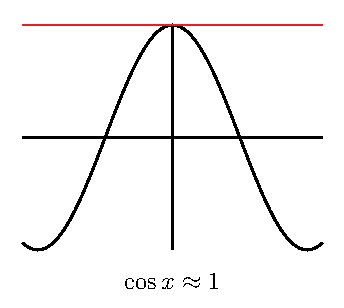
\includegraphics{approx1d} \qquad\qquad
  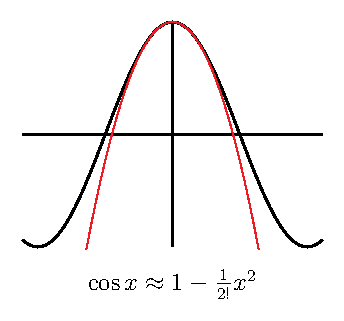
\includegraphics{approx2d}
\end{center}
\begin{center}
  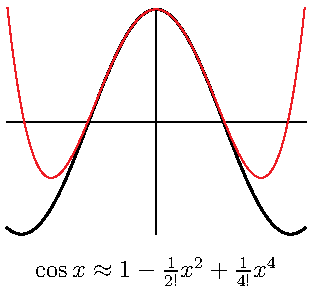
\includegraphics{approx3d} \qquad\qquad
  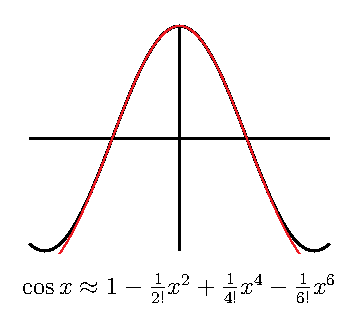
\includegraphics{approx4d}
\end{center}
\end{efig}

\end{eg}
The above work is quite easily recycled to get the Maclaurin polynomial for sine:
\begin{eg}\label{eg expand sinx}
 Find the 5th degree Maclaurin polynomial for $\sin x$.

\soln We could simply work as before and compute the first five derivatives of $\sin x$.
But set $g(x) = \sin x$ and notice that $g(x) = - f'(x)$, where $f(x) =\cos x$. Then we
have
\begin{align*}
  g(0) &= -f'(0) = 0 \\
  g'(0) &= -f''(0) = 1\\
  g''(0) &= -f'''(0) = 0\\
  g'''(0) &= -f^{(4)}(0) = -1\\
  g^{(4)}(0) &= -f^{(5)}(0) = 0\\
  g^{(5)}(0) &= -f^{(6)}(0) = 1
\end{align*}
Hence the required Maclaurin polynomial is
\begin{align*}
  T_5(x) &= x - \frac{x^3}{3!} + \frac{x^5}{5!}
\end{align*}
Just as we extended to the $2n^\mathrm{th}$ Maclaurin polynomial for cosine, we can also
extend our work to compute the $(2n+1)^\mathrm{th}$ Maclaurin polynomial for sine:
\begin{align*}
  T_{2n+1}(x) &= \sum_{k=0}^n \frac{(-1)^k}{(2k+1)!} \cdot x^{2k+1}
\end{align*}
\begin{warning}
The above formula only works when x is measured in radians, because all of our
derivative formulae for trig functions were developed under the assumption that
angles are measured in radians.
\end{warning}


Below we plot $\sin x$ against its first few Maclaurin polynomial approximations.
\begin{efig}
\begin{center}

  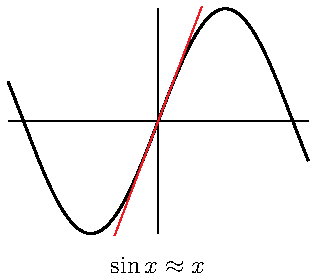
\includegraphics{approx1c} \qquad\qquad
  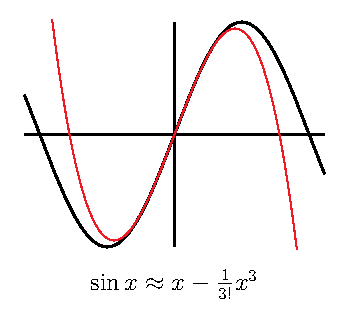
\includegraphics{approx2c}
\end{center}
\begin{center}
  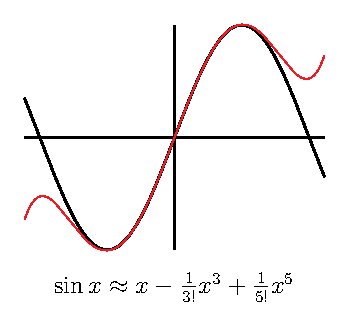
\includegraphics{approx3c} \qquad\qquad
  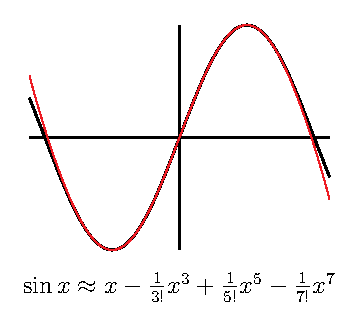
\includegraphics{approx4c}
\end{center}
\end{efig}

\end{eg}

To get an idea of how good these Taylor polynomials are at approximating $\sin$ and
$\cos$, let's concentrate on $\sin x$ and consider $x$'s whose magnitude $|x|\le 1$.
There are tricks that you can employ\footnote{If you are writing software to evaluate
$\sin x$, you can always use the trig identity $\sin(x)=\sin(x-2n\pi)$, to  easily
restrict to $|x|\le\pi$. You can then use the trig identity $\sin(x)=-\sin(x\pm\pi)$ to
reduce to $|x|\le\tfrac{\pi}{2}$. Finally you can use the trig identity
$\sin(x)=\mp\cos(\tfrac{\pi}{2}\pm x))$ to reduce to $|x|\le\tfrac{\pi}{4} < 1$.} to
evaluate sine and cosine at values of $x$ outside this range.

If $|x|\le 1$ radians\footnote{Recall that the derivative formulae that we used to
derive the Taylor polynomials are valid only when $x$ is in radians. The
restriction $-1 \leq x \leq 1$ radians translates to angles bounded by
$\tfrac{180}{\pi}\approx 57^\circ$.}, then the magnitudes of the successive
terms in the Taylor polynomials for $\sin x$ are bounded by
\begin{align*}
|x|&\le 1 &
\tfrac{1}{3!}|x|^3&\le\tfrac{1}{6} &
\tfrac{1}{5!}|x|^5&\le\tfrac{1}{120}\approx 0.0083 \\
\tfrac{1}{7!}|x|^7&\le\tfrac{1}{7!}\approx 0.0002 &
\tfrac{1}{9!}|x|^9&\le\tfrac{1}{9!}\approx 0.000003 &
\tfrac{1}{11!}|x|^{11}&\le\tfrac{1}{11!}\approx 0.000000025
\end{align*}
From these inequalities, and the graphs on the previous pages, it certainly looks like,
for $x$ not too large, even relatively low degree Taylor polynomials give very good
approximations. In Section~\ref{ssec taylor error} we'll see how to get rigorous error
bounds on our Taylor polynomial approximations.




%%%%%%%%%%%%%%%%%%%%%%%%%%%%%%%%%%%%%%%%%%%%%%%%%%%%%%%%%%%%%%%%%%%%%%
\subsection{Estimating Change and $\De x$, $\De y$ Notation}
%%%%%%%%%%%%%%%%%%%%%%%%%%%%%%%%%%%%%%%%%%%%%%%%%%%%%%%%%%%%%%%%%%%%%%


Suppose that we have two variables $x$ and $y$ that are related by $y=f(x)$, for some
function $f$. One of the most important applications of calculus is to help us understand
what happens to $y$ when we make a small change in $x$.

\begin{notn}
 Let $x,y$ be variables related by a function $f$. That is $y = f(x)$. Then we denote a
  small change in the variable $x$ by $\De x$ (read as ``delta $x$''). The corresponding
small change in the variable $y$ is denoted $\De y$ (read as ``delta $y$'').
\begin{align*}
  \De y &= f(x+\De x) - f(x)
\end{align*}
\end{notn}

In many situations we do not need to compute $\De y$ exactly and are instead happy with
an approximation. Consider the following example.
\begin{eg}
Let $x$ be the number of cars manufactured per week in some factory and let $y$ the cost
of manufacturing those $x$ cars. Given that the factory currently produces $a$ cars per
week, we would like to estimate the increase in cost if we make a small change in the
number of cars produced.

\soln We are told that $a$ is the number of cars currently produced per week; the cost
of production  is then $f(a)$.
\begin{itemize}
 \item Say the number of cars produced is changed from $a$ to $a+\De x$ (where $\De x$
is some small number.
\item As $x$ undergoes this change, the costs change from $y=f(a)$ to $f(a+\De x)$.
Hence
\begin{align*}
  \De y &= f(a+\De x) - f(a)
\end{align*}
\item We can estimate this change using a linear approximation. Substituting
$x=a+\De x$ into the equation~\eqref{eq:linApprox} yields the approximation
\begin{align*}
f(a+\De x)\approx f(a)+f'(a)(a+\De x-a)
\end{align*}
and consequently the approximation
\begin{align*}
\De y=f(a+\De x)-f(a)\approx f(a)+f'(a)\De x-f(a)
\end{align*}
simplifies to the following neat estimate of $\De y$:
\begin{impeqn}[Linear approximation of $\De y$]\label{eq:lineDe}
\begin{align*}
    \De y\approx f'(a)\De x
\end{align*}
\end{impeqn}
\item In the automobile manufacturing example, when the production level is $a$ cars per
week, increasing the production level by $\De x$ will cost approximately
$f'(a)\De x$. The additional cost per additional car, $f'(a)$,  is called the ``marginal
cost'' of a car.

\item If we instead use the quadratic approximation (given by
equation~\eqref{eq:quadApprox}) then we estimate
\begin{align*}
f(a+\De x)\approx f(a)+f'(a)\De x+\half f''(a)\De x^2
\end{align*}
and so
\begin{align*}
\De y&=f(a+\De x)-f(a) \approx f(a)+f'(a)\De x +\half f''(a)\De x^2-f(a)
\end{align*}
which simplifies to
\begin{impeqn}[Quadratic approximation of $\De y$]\label{eq:quadDe}
\begin{align*}
  \De y &\approx f'(a)\De x+\half f''(a)\De x^2
\end{align*}
\end{impeqn}
\end{itemize}

\end{eg}

%%%%%%%%%%%%%%%%%%%%%%%%%%%%%%%%%%%%%%%%%%%%%%%%%%%%%%%%%%%%%%%%%%%%%%
\subsection{Further Examples}
%%%%%%%%%%%%%%%%%%%%%%%%%%%%%%%%%%%%%%%%%%%%%%%%%%%%%%%%%%%%%%%%%%%%%%
In this subsection we give further examples of computation and use of Taylor
approximations.

\begin{eg}\label{eg:taylorapprox}
Estimate $\tan 46^\circ$, using the constant-, linear- and quadratic-approximations
(equations~\eqref{eq:constApprox}, \eqref{eq:linApprox} and~\eqref{eq:quadApprox}).

\soln Note that we need to be careful to translate angles measured in degrees to radians.
\begin{itemize}
 \item Set $f(x)=\tan x$, $x=46\tfrac{\pi}{180}$ radians
and $a=45\tfrac{\pi}{180}=\tfrac{\pi}{4}$ radians.
This is a good choice for $a$ because
\begin{itemize}
\item  $a=45^\circ$ is close to $x=46^\circ$. As noted above, it is generally the case
that the closer $x$ is to $a$, the better various approximations will be.
\item We know the values of all trig functions at $45^\circ$.
\end{itemize}
\item Now we need to compute $f$ and its first two derivatives at $x=a$. It is a good
time to recall the special $1:1:\sqrt{2}$ triangle
\begin{efig}
 \begin{center}
  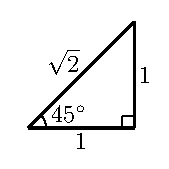
\includegraphics{triangle45}
 \end{center}
\end{efig}
So
\begin{align*}
  f(x) &= \tan x & f(\pi/4) &= 1\\
%
  f'(x) &= \sec^2 x = \frac{1}{\cos^2 x}
  & f'(\pi/4) &= \frac{1}{1/\sqrt{2}^2} = 2 \\
%
  f''(x) &=  \frac{2\sin x}{\cos^3 x}
  & f''(\pi/4) &= \frac{2/\sqrt{2}}{1/\sqrt{2}^3} = 4
\end{align*}
\item As $x-a=46\tfrac{\pi}{180}-45\tfrac{\pi}{180}=\tfrac{\pi}{180}$ radians, the
three approximations are
\begin{alignat*}{3}
f(x)&\approx f(a) &
    &&&=1\\
f(x)&\approx f(a)+f'(a)(x-a) &
    &=1+2\tfrac{\pi}{180} &
    &=1.034907\\
f(x)&\approx f(a)+f'(a)(x-a)+\half f''(a)(x-a)^2&
    &=1+2\tfrac{\pi}{180}+\half 4\big(\tfrac{\pi}{180}\big)^2 &
    & =1.035516
\end{alignat*}
For comparison purposes, $\tan 46^\circ$ really is $1.035530$ to 6 decimal
places.

\end{itemize}

\end{eg}

\begin{warning}\label{warning:radians}
All of our derivative formulae for trig functions were developed under
the assumption that angles are measured in radians.
Those derivatives appeared in the approximation formulae that we used
in Example \ref{eg:taylorapprox}, so we were obliged to express $x-a$
in radians.
\end{warning}


\begin{comment}
\begin{eg}\label{eg:taylorSinCos}
Let's find all Taylor polynomials for $\sin x$ and $\cos x$ at $x=a=0$.
To do so we merely need compute all derivatives of $\sin x$ and  $\cos x$
at $x=0$. First, compute all derivatives at general $x$.
\begin{equation}\label{eq:sinCosDerivs}
\begin{aligned}
f(x)&=\sin x &
f'(x)&=\cos x &
f''(x)&=-\sin x &
f^{(3)}(x)&=-\cos x &
f^{(4)}(x)&=\sin x & \cdots\\
g(x)&=\cos x &
g'(x)&=-\sin x &
g''(x)&=-\cos x &
g^{(3)}(x)&=\sin x &
g^{(4)}(x)&=\cos x & \cdots
\end{aligned}
\end{equation}
The pattern starts over again with the fourth derivative being the same
as the original function. Now set $x=a=0$.
\begin{equation}\label{eq:sinCosDerivsZero}
\begin{aligned}
f(x)&=\sin x &
f(0)&=0 &
f'(0)&=1 &
f''(0)&=0 &
f^{(3)}(0)&=-1 &
f^{(4)}(0)&=0 & \cdots\\
g(x)&=\cos x &
g(0)&=1 &
g'(0)&=0 &
g''(0)&=-1 &
g^{(3)}(0)&=0 &
g^{(4)}(0)&=1 & \cdots
\end{aligned}
\end{equation}
For $\sin x$, all even numbered derivatives are zero. The odd numbered
derivatives alternate between $1$ and $-1$.
For $\cos x$, all odd numbered derivatives are zero. The even numbered
derivatives alternate between $1$ and $-1$. So, the Taylor polynomials
that best approximate $\sin x$ and $\cos x$ near $x=a=0$ are
\begin{align*}
\sin x &\approx x-\tfrac{1}{3!}x^3+\tfrac{1}{5!}x^5-\cdots\\
\cos x &\approx 1-\tfrac{1}{2!}x^2+\tfrac{1}{4!}x^4-\cdots
\end{align*}
Here are graphs of $\sin x$ and its Taylor polynomials (about $x=a=0$)
up to degree seven.
\begin{efig}
\begin{center}

  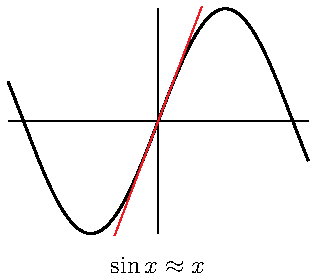
\includegraphics{approx1c} \qquad\qquad
  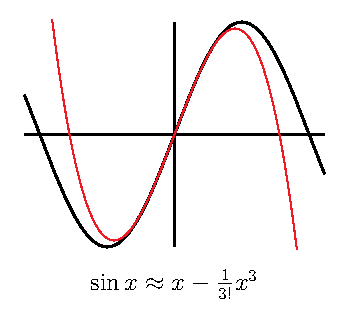
\includegraphics{approx2c}
\end{center}
\begin{center}
  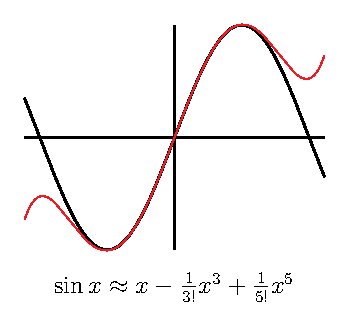
\includegraphics{approx3c} \qquad\qquad
  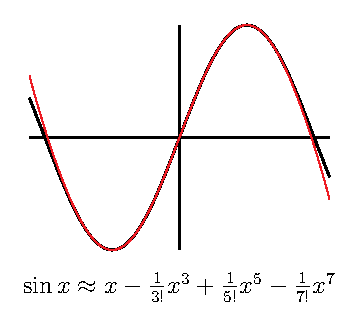
\includegraphics{approx4c}
\end{center}
\end{efig}
To get an idea of how good these Taylor polynomials are at
approximating $\sin$ and $\cos$, let's concentrate on $\sin x$ and consider
$x$'s whose magnitude $|x|\le 1$. (If you're writing software to evaluate
$\sin x$, you can always use the trig identity
$\sin(x)=\sin(x-2n\pi)$, to  easily restrict to $|x|\le\pi$, and then use
the trig identity $\sin(x)=-\sin(x\pm\pi)$ to reduce to $|x|\le\tfrac{\pi}{2}$
and then use the trig identity $\sin(x)=\mp\cos(\tfrac{\pi}{2}\pm x))$
to reduce to $|x|\le\tfrac{\pi}{4}$.) If $|x|\le 1$ radians (recall that
the derivative formulae that we used to derive the Taylor polynomials are
valid only when $x$ is in radians), or equivalently if $|x|$ is no larger
than $\tfrac{180}{\pi}\approx 57^\circ$, then the magnitudes of the successive
terms in the Taylor polynomials for $\sin x$ are bounded by
\begin{align*}
|x|&\le 1 &
\tfrac{1}{3!}|x|^3&\le\tfrac{1}{6} &
\tfrac{1}{5!}|x|^3&\le\tfrac{1}{120}\approx 0.0083 \\
\tfrac{1}{7!}|x|^7&\le\tfrac{1}{7!}\approx 0.0002 &
\tfrac{1}{9!}|x|^9&\le\tfrac{1}{9!}\approx 0.000003 &
\tfrac{1}{11!}|x|^{11}&\le\tfrac{1}{11!}\approx 0.000000025
\end{align*}
From these inequalities, and the graphs on the previous page, it
certainly looks like, for $x$ not too large, even relatively low degree
Taylor polynomials give very good approximations.
We'll see later how to get rigorous error bounds on our Taylor polynomial
approximations.
\end{eg}

\end{comment}

\begin{eg}\label{eg:taylorPole}
Suppose that you are ten meters from a vertical pole. You were
contracted to measure the height of the pole. You can't
take it down or climb it. So you measure the angle subtended by
the top of the pole. You measure $\theta=30^\circ$,  which gives
\begin{align*}
h=10\tan 30^\circ=\tfrac{10}{\sqrt{3}}\approx 5.77\text{m}\qquad\qquad
\end{align*}
This is just standard trigonometry ---  if we know the angle exactly then we know the
height exactly.

However, in the ``real world'' angles are hard to measure with such precision. If the
contract requires you the measurement of the pole to be accurate within $10$ cm, how
accurate does your measurement of the angle $\theta$ need to be?

\soln For simplicity\footnote{Mathematicians love assumptions that let us tame the real
world.}, we are going to assume that the pole is perfectly straight
and perfectly vertical and that your distance from the pole was exactly
10 m.
\begin{itemize}
\item Write $\theta=\theta_0+\De\theta$ where $\theta$ is the exact angle, $\theta_0$ is
the measured angle and $\De \theta$ is the error.
\item Similarly write $h=h_0+\De h$, where $h$ is the exact height and
$h_0=\tfrac{10}{\sqrt{3}}$ is the computed height. Their difference,
$\De h$, is the error.

\item Then
\begin{align*}
h_0&=10\tan\theta_0 & h_0+\De h&=10\tan(\theta_0+\De\theta)\\
\De h &= 10\tan(\theta_0+\De\theta) - 10\tan\theta_0
\end{align*}
We could attempt to solve this equation for $\De\theta$ in terms of $\De h$ --- but it is
far simpler to approximate $\De h$ using the linear approximation in
equation~\ref{eq:lineDe}.

\item To use equation~\ref{eq:lineDe}, replace $y$ with $h$, $x$ with $\theta$ and $a$
with $\theta_0$. Our function $f(\theta) = 10 \tan\theta$ and $\theta_0 = 30^\circ =
\pi/6$ radians. Then
\begin{align*}
  \De y &\approx f'(a) \De x & \text{ becomes }&&
  \De h &\approx f'(\theta_0) \De \theta
\end{align*}
Since $f(\theta)=10 \tan \theta$, $f'(\theta) = 10\sec^2\theta$ and
\begin{align*}
  f'(\theta_0) = 10\sec^2(\pi/6)
  = 10 \cdot \left(\frac{2}{\sqrt{3}} \right)^2 = \frac{40}{3}
\end{align*}

\item Putting things together gives
\begin{align*}
  \De h &\approx f'(\theta_0) \De \theta & \text{ becomes }&&
  \De h & \approx \frac{40}{3} \De \theta
\end{align*}
We can then solve this equation for $\De\theta$ in terms of $\De h$:
\begin{align*}
  \De \theta & \approx \frac{3}{40} \De h
\end{align*}

\item We are told that we must have $|\De h| < 0.1$, so we must have
\begin{align*}
  |\De \theta| &\leq \frac{3}{400}
\end{align*}
This is measured in radians, so converting back to degrees
\begin{align*}
  \frac{3}{400} \cdot \frac{180}{\pi} &= 0.43^\circ
\end{align*}

\end{itemize}

\end{eg}
\goodbreak

\begin{defn}\label{def:APPrelError} %%%%%%%%%%%%%%%%%%%%%
    Suppose that you measure, approximately, some quantity.
    Suppose that the exact value of that quantity is $Q_0$
    and that your measurement yielded $Q_0+\De Q$. Then
    $|\De Q|$ is called the absolute error of the measurement
    and $100\frac{|\De Q|}{Q_0}$ is called the percentage error
    of the measurement. As an example, if the exact
    value is $4$ and the measured value is $5$, then the absolute
    error is $|5-4|=1$ and the percentage error is
    $100\frac{|5-4|}{4}=25$. That is, the error, $1$, was $25\%$
    of the exact value, $4$.
\end{defn}


\begin{eg}\label{eg:taylorSphere}
Suppose that the radius of a sphere has been
measured with a percentage error of at most $\veps$\%. Find
the corresponding approximate percentage errors in the surface
area and volume of the sphere.

\soln We need to be careful in this problem to convert between absolute and percentage
errors correctly.

\begin{itemize}
\item Suppose that the exact radius is $r_0$ and that the measured radius is $r_0+\De r$.
\item Then the absolute error in the measurement is $|\De r|$ and, by definition, the
percentage error is $100\tfrac{|\De r|}{r_0}$. We are told that $100\tfrac{|\De
r|}{r_0}\le\veps$.

\item The surface area\footnote{We do not expect you to remember the surface areas of
solids for this course.} of a sphere of radius $r$ is $A(r)=4\pi r^2$. The error
in the surface area computed with the measured radius is
\begin{align*}
\De A &=A(r_0+\De r)-A(r_0)\approx A'(r_0)\De r\\
&= 8\pi r_0 \Delta r
\end{align*}
where we have made use of the linear approximation, equation~\eqref{eq:lineDe}.

\item The corresponding percentage error is then
\begin{align*}
100\frac{|\De A|}{A(r_0)}
\approx 100\frac{|A'(r_0)\De r|}{A(r_0)}
= 100\frac{8\pi r_0|\De r|}{4\pi r_0^2}
= 2\times 100\frac{|\De r|}{r_0}
\le 2\veps
\end{align*}


\item The volume of a sphere\footnote{We do expect you to remember the formula for the
volume of a sphere.} of radius $r$ is $V(r)=\frac{4}{3}\pi r^3$. The error in the volume
computed with the measured radius is
\begin{align*}
\De V &=V(r_0+\De r)-V(r_0)\approx V'(r_0)\De r \\
  &= 4\pi r_0^2 \Delta r
\end{align*}
where we have again made use of the linear approximation, equation~\eqref{eq:lineDe}.

\item The corresponding percentage error is
\begin{align*}
100\frac{|\De V|}{V(r_0)}
\approx 100\frac{|V'(r_0)\De r|}{V(r_0)}
= 100\frac{4\pi r_0^2|\De r|}{4\pi r_0^3/3}
= 3\times 100\frac{|\De r|}{r_0}
\le 3\veps
\end{align*}
\end{itemize}
We have just computed an approximation to $\Delta V$. This problem is actually
sufficiently simple that we can compute $\Delta V$ exactly:
\begin{align*}
  \Delta V &=  V(r_0 + \Delta r) - V(r_0)
	    = \tfrac{4}{3} \pi (r_0 + \Delta r)^3
	      - \tfrac{4}{3} \pi r_0^3
\end{align*}
\begin{itemize}
 \item Applying $(a+b)^3=a^3+3a^2b+3ab^2+b^3$ with $a=r_0$ and $b=\De r$, gives
\begin{align*}
V(r_0+\De r)-V(r_0)&=\tfrac{4}{3}\pi
\left[r_0^3+3r_0^2\De r+3r_0\,(\De r)^2+(\De r)^3\right] - \tfrac{4}{3}\pi  r_0^3\\
&=\tfrac{4}{3}\pi[3r_0^2\De r+3r_0\,(\De r)^2+(\De r)^3]
\end{align*}

\item Thus the difference between the exact error and the linear approximation
to the error is obtained by retaining only the last two terms in the square brackets. This
has magnitude
\begin{align*}
\tfrac{4}{3}\pi\big|3r_0\,(\De r)^2+(\De r)^3\big|
=\tfrac{4}{3}\pi\big|3r_0+\De r\big|(\De r)^2
\end{align*}
or in percentage terms
\begin{align*}
100\cdot \dfrac{1}{\tfrac{4}{3}\pi r_0^3} \cdot
\tfrac{4}{3}\pi \big|3r_0\,(\De r)^2+(\De r)^3\big|
%
&=100\left|3\frac{\De r^2}{r_0^2}+\frac{\De r^3}{r_0^3}\right|\\
%
&=\left(100 \frac{3\De r}{r_0}\right)
\cdot \left(\frac{\De r}{r_0}\right)
\left|1 +\frac{\De r}{3r_0}\right|\\
%
& \le 3\veps \left(\frac{\veps}{100}\right)\cdot \left(1+\frac{\veps}{300}\right)
\end{align*}
Since $\veps$ is small, we can assume that $1 + \frac{\veps}{300} \approx 1$. Hence the
difference between the exact error and the linear approximation of the error is roughly a
factor of $\tfrac{\veps}{100}$ smaller than the linear approximation $3\veps$.


\item As an aside, notice that if we argue that $\De r$ is very small and so we
can ignore terms involving $(\De r)^2$ and $(\De r)^3$ as being really really
small, then we obtain
\begin{align*}
V(r_0+\De r)-V(r_0)
&=\tfrac{4}{3}\pi[3r_0^2\De r \underbrace{+3r_0\,(\De r)^2+(\De
r)^3}_\text{really
really small}]\\
&\approx \tfrac{4}{3}\pi \cdot 3r_0^2\De r  = 4 \pi r_0^2 \De r
\end{align*}
which is precisely the result of our linear approximation above.


\end{itemize}
\end{eg}
\goodbreak

\begin{eg}\label{eg:taylorLamp}
To compute the height $h$ of a lamp post, the length $s$ of the
shadow of a two meter pole is measured. The pole is 6 m from the lamp post.
If the length of the shadow was measured to be 4 m, with an error of
at most one cm, find the height of the lamp post and estimate the
percentage error in the height.

\soln We should first draw a picture\footnote{We get to reuse that nice lamp post picture
from Example~\ref{eg:fallingBall}.}
\begin{efig}
 \begin{center}
  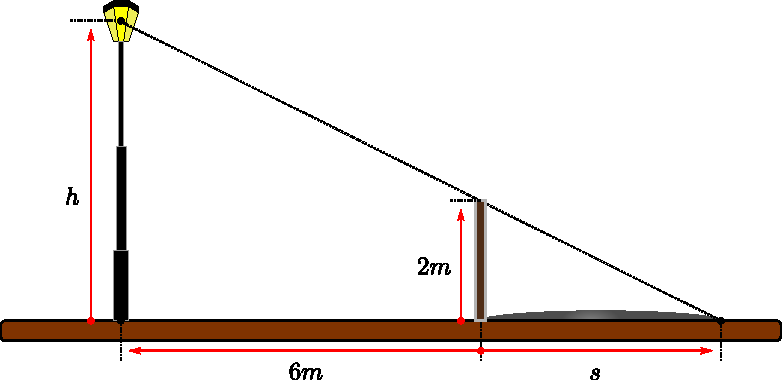
\includegraphics[height=6cm]{extra/lamp_shadow}
 \end{center}
\end{efig}
\begin{itemize}
\item By similar triangles we see that
\begin{align*}
    \frac{2}{s} &= \frac{h}{6+s}
\end{align*}
from which we can isolate $h$ as a function of $s$:
\begin{align*}
  h &= \frac{2(6+s)}{s} = \frac{12}{s} + 2
\end{align*}
\item The length of the shadow was measured to be $s_0=4$ m. The corresponding
height of the lamp post is
\begin{align*}
  h_0 &= \frac{12}{4} + 2 = 5m
\end{align*}

\item If the error in the measurement of the length of the shadow was $\De s$, then the
exact shadow length was $s=s_0+\De s$ and the exact lamp post height is $h=f(s_0+\De s)$,
where $f(s)=\tfrac{12}{s}+2$. The error in the computed lamp post height is
\begin{align*}
  \De h=h-h_0=f(s_0+\De s)-f(s_0)
\end{align*}

\item We can then make a linear approximation of this error using
equation~\eqref{eq:lineDe}:
\begin{align*}
\De h &\approx f'(s_0)\De s =-\frac{12}{s_0^2}\De s =-\frac{12}{4^2}\De s
\end{align*}
\item We are told that $|\De s|\le\frac{1}{100}$ m. Consequently, approximately,
\begin{align*}
 |\De h|\le \frac{12}{4^2}\frac{1}{100}=\frac{3}{400}
\end{align*}
The percentage error is then approximately
\begin{align*}
  100\frac{|\De h|}{h_0} & \le 100\frac{3}{400\times 5}=0.15\%
\end{align*}
\end{itemize}
\end{eg}

% \begin{eg}\label{eg:taylorPlane}
% \issue{Joel:\\ Replace\\ this?}
% When an aircraft crosses the Atlantic ocean at a speed of $u$ mph, the
% flight costs the company
% \begin{align*}
% C(u)=100+\tfrac{u}{3}+\tfrac{240,000}{u}
% \end{align*}
% dollars per passenger.
% When there is no wind, the aircraft flies at an airspeed of $550$mph.
% Find the approximate savings, per passenger, when there is a
% $35$ mph tail wind and estimate the cost when there is a $50$ mph head wind.
%
% \soln
% Let $u_0=550$. When the aircraft flies at speed $u_0$, the cost per passenger
% is $C(u_0)$. By \eqref{eq:lineDe}, a change of $\De u$ in the airspeed
% results in an change of
% \begin{align*}
% \De C\approx C'(u_0)\De u
% =\big[\tfrac{1}{3}-\tfrac{240,000}{u_0^2}\big]\De u
% =\big[\tfrac{1}{3}-\tfrac{240,000}{550^2}\big]\De u
% \approx-.460\De u
% \end{align*}
% in the cost per passenger. With the tail wind $\De u=35$ and the resulting
% \begin{align*}
% \De C\approx -.460\times 35=-16.10
% \end{align*}
% so there is a savings of $\$16.10$. With the head wind $\De u=-50$ and
% the resulting
% \begin{align*}
% \De C\approx -.4601\times (-50)=23.01
% \end{align*}
% so there is an additional cost of about $\$23.00$.
% \end{eg}
%

\goodbreak



%%%%%%%%%%%%%
\subsection{The Error in the Taylor Polynomial Approximations}\label{ssec taylor error}
%%%%%%%%%%%%%%
Any time you make an approximation, it is desirable to have some idea
of the size of the error you introduced. That is, we would like to know the difference
$R(x)$ between the original function $f(x)$ and our approximation $F(x)$:
\begin{align*}
  R(x) &= f(x)-F(x).
\end{align*}
Of course if we know $R(x)$ exactly, then we could recover $f(x) = F(x)+R(x)$ --- so this
is an unrealistic hope. In practice we would simply like to bound $R(x)$:
\begin{align*}
  |R(x)| &= |f(x)-F(x)| \leq M
\end{align*}
where (hopefully) $M$ is some small number. It is worth stressing that we do not need the
tightest possible value of $M$, we just need a relatively easily computed $M$ that isn't
too far off the true value of $|f(x)-F(x)|$.


We will now develop a formula for the error introduced by the constant approximation,
equation~\eqref{eq:constApprox} (developed back in Section~\ref{ssec const
approx})
\begin{align*}
f(x)&\approx f(a) = T_0(x) & \text{$0^\mathrm{th}$ Taylor polynomial}
\end{align*}
The resulting formula can be used to get an upper bound on the size of the error
$|R(x)|$.

The main ingredient we will need is the Mean-Value Theorem (Theorem~\ref{thm:DIFFmvt})
--- so we suggest you quickly revise it. Consider the following obvious statement:
\begin{align*}
  f(x) &= f(x) & \text{now some sneaky manipulations}\\
  & = f(a) + (f(x)-f(a)) \\
  &= \underbrace{f(a)}_{=T_0(x)} + (f(x)-f(a)) \cdot \underbrace{\frac{x-a}{x-a}}_{=1} \\
  &= T_0(x) + \underbrace{\frac{f(x)-f(a)}{x-a}}_\text{looks familiar} \cdot (x-a)
\end{align*}
Indeed, this equation is important in the discussion that follows, so we'll highlight it
\begin{impeqn}[We will need it again soon]\label{eq:taylorErrorA}
 \begin{align*}
  f(x) &= T_0(x) + \left[ \frac{f(x)-f(a)}{x-a} \right](x-a)
 \end{align*}
\end{impeqn}
The coefficient $\dfrac{f(x)-f(a)}{x-a}$ of $(x-a)$ is the average slope
of $f(t)$ as $t$ moves from $t=a$ to $t=x$. We can picture this as the slope of the
secant joining the points $(a,f(a))$ and $(x,f(x))$ in the sketch below.
\vadjust{
  \begin{efig}
  \begin{center}
     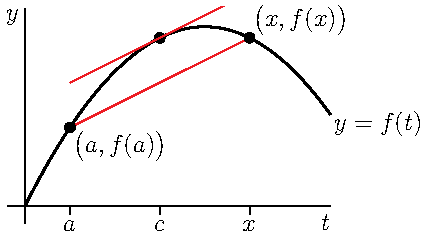
\includegraphics{approx4bb}
  \end{center}
  \end{efig}
}

As $t$ moves from $a$ to $x$, the instantaneous slope $f'(t)$ keeps changing. Sometimes
$f'(t)$ might be larger than the average slope $\tfrac{f(x)-f(a)}{x-a}$, and sometimes
$f'(t)$ might be smaller than the average slope $\tfrac{f(x)-f(a)}{x-a}$. However, by the
Mean-Value Theorem (Theorem~\ref{thm:DIFFmvt}), there must be some number $c$, strictly
between $a$ and $x$, for which  $f'(c)=\dfrac{f(x)-f(a)}{x-a}$ exactly.


Substituting this into formula \eqref{eq:taylorErrorA} gives
\begin{impeqn}[Towards the error]\label{eq:taylorErrorL}
\begin{align*}
  f(x) &=T_0(x) +f'(c)(x-a) & \text{for some $c$ strictly between $a$ and $x$}
\end{align*}
\end{impeqn}
Notice that this expression as it stands is not quite what we want. Let us massage this
around a little more into a more useful form
\begin{impeqn}[The error in constant approximation]\label{eq:taylorErrorL2}
 \begin{align*}
  f(x) - T_0(x) &= f'(c) \cdot (x-a) & \text{for some $c$ strictly between
$a$ and $x$}
\end{align*}
\end{impeqn}
Notice that the MVT doesn't tell us the value of $c$, however we do know that it lies
strictly between $x$ and $a$. So if we can get a good bound on $f'(c)$ on this interval
then we can get a good bound on the error.

\begin{eg}\label{eg zero approx of e}
  Let us return to Example~\ref{eg ex const approx}, and we'll try to bound the error in
our approximation of~$e^{0.1}$.

\begin{itemize}
 \item Recall that $f(x) = e^x$, $a=0$ and $T_0(x) = e^0 = 1$.
 \item Then by equation~\eqref{eq:taylorErrorL2}
  \begin{align*}
    e^{0.1} - T_0(0.1) &= f'(c) \cdot (0.1 - 0) & \text{with $0<c<0.1$}
  \end{align*}
  \item Now $f'(c) = e^c$, so we need to bound $e^c$ on $(0,0.1)$. Since $e^c$ is an
  increasing function, we know that
  \begin{align*}
    e^0 &< f'(c) < e^{0.1}  & \text{ when $0<c<0.1$}
  \end{align*}
  So one is tempted to write that
  \begin{align*}
    |e^{0.1} - T_0(0.1)| &= |R(x)| = |f'(c)| \cdot (0.1 - 0)\\
    & < e^{0.1} \cdot 0.1
  \end{align*}
  And while this is true, it is rather circular. We have just bounded the error in our
  approximation of $e^{0.1}$ by $\frac{1}{10}e^{0.1}$ --- if we actually knew $e^{0.1}$
  then we wouldn't need to estimate it!

  \item While we don't know $e^{0.1}$ exactly, we do know\footnote{Oops! Do we
really know that $e<3$? We haven't proved it. We will do so soon.}
that $1 = e^0 < e^{0.1} < e^1 <
3$. This   gives us
  \begin{align*}
    |R(0.1)| < 3 \times 0.1 = 0.3
  \end{align*}
  That is --- the error in our approximation of $e^{0.1}$ is no greater than $0.3$.
  Recall that we don't need the error exactly, we just need a good idea of how large it
  actually is.

  \item In fact the real error here is
\begin{align*}
  |e^{0.1} - T_0(0.1)| &=|e^{0.1} - 1| = 0.1051709\dots
\end{align*}
so we have over-estimated the error by a factor of 3.
\end{itemize}

But we can actually go a little further here --- we can bound the error above and below.
If we do not take absolute values, then since
  \begin{align*}
    e^{0.1} - T_0(0.1) &= f'(c) \cdot 0.1 & \text{ and } 1 < f'(c) < 3
  \end{align*}
we can write
\begin{align*}
  1\times 0.1 \leq ( e^{0.1} - T_0(0.1) ) & \leq 3\times 0.1
\end{align*}
so
\begin{align*}
  T_0(0.1) + 0.1 &\leq e^{0.1} \leq T_0(0.1)+0.3 \\
  1.1 &\leq e^{0.1} \leq 1.3
\end{align*}
So while the upper bound is weak, the lower bound is quite tight.

\end{eg}

There are formulae similar to equation~\eqref{eq:taylorErrorL}, that can be used to bound
the error in our other approximations; all are based on generalisations of the
MVT. The
next one --- for linear approximations --- is
\begin{align*}
f(x) & =\underbrace{f(a)+f'(a)(x-a)}_{=T_1(x)}+\half f''(c)(x-a)^2 &
\text{for some $c$ strictly between $a$ and $x$}
\end{align*}
which we can rewrite in terms of $T_1(x)$:
\begin{impeqn}[The error in linear approximation]\label{eq:taylorErrorQ}
\begin{align*}
f(x)-T_1(x) &=  \half f''(c)(x-a)^2 & \text{for some $c$ strictly between $a$ and $x$}
\end{align*}
\end{impeqn}
It implies that the error that we make when we approximate $f(x)$ by
$T_1(x) = f(a)+f'(a)\,(x-a)$ is exactly $\half f''(c)\,(x-a)^2$ for some $c$ strictly
between $a$ and $x$.


More generally
\begin{align*}
f(x)=&
\underbrace{f(a)+f'(a)\cdot(x-a)+\cdots+\frac{1}{n!}f^{(n)}(a)\cdot(x-a)^n}_{= T_n(x)}
+\frac{1}{(n+1)!}f^{(n+1)}(c)\cdot (x-a)^{n+1}
\end{align*}
for some $c$ strictly between $a$ and $x$. Again, rewriting this in terms of $T_n(x)$
gives
\begin{impeqn}\label{eq:taylorErrorN}
\begin{align*}
  f(x) - T_n(x) &= \frac{1}{(n+1)!}f^{(n+1)}(c)\cdot (x-a)^{n+1}
& \text{for some $c$ strictly between $a$ and $x$}
\end{align*}
\end{impeqn}

That is, the error introduced when $f(x)$ is approximated by its Taylor
polynomial of degree $n$, is precisely the last term of the Taylor polynomial
of degree $n+1$, but with the derivative evaluated at some point between
$a$ and $x$, rather than exactly at $a$. These error formulae are proven
in the optional Section~\ref{subsec:GMVT} later in this chapter.


\begin{eg}\label{eg:taylorErrorSin}
Approximate $\sin 46^\circ$ using Taylor polynomials about
$a=45^\circ$, and estimate the resulting error.

\soln
\begin{itemize}
 \item Start by defining $f(x) = \sin x$ and
\begin{align*}
a&=45^\circ=45\tfrac{\pi}{180} {\rm radians}&
x&=46^\circ=46\tfrac{\pi}{180} {\rm radians}&
x-a&=\tfrac{\pi}{180} {\rm radians}
\end{align*}
\item The first few derivatives of $f$ at $a$ are
\begin{alignat*}{2}
f(x)&=\sin x
&f(a)&=\frac{1}{\sqrt{2}}\\
f'(x)&=\cos x &
f'(a)&=\frac{1}{\sqrt{2}}\\
f''(x)&=-\sin x &
f''(a)&=-\frac{1}{\sqrt{2}}\\
f^{(3)}(x)&=-\cos x &
f^{(3)}(a)&=-\frac{1}{\sqrt{2}}
\end{alignat*}
\item
The constant, linear and quadratic Taylor approximations for $\sin(x)$ about
$\frac{\pi}{4}$ are
\begin{alignat*}{4}
  T_0(x) &= f(a)
    &&= \frac{1}{\sqrt{2}} \\
  T_1(x) &= T_0(x) + f'(a) \cdot(x-a)
    &&= \frac{1}{\sqrt{2}} + \frac{1}{\sqrt{2}}\left(x - \frac{\pi}{4} \right)\\
  T_2(x) &= T_1(x) + \half f''(a) \cdot(x-a)^2
    &&=  \frac{1}{\sqrt{2}} + \frac{1}{\sqrt{2}}\left(x - \frac{\pi}{4} \right)
  - \frac{1}{2\sqrt{2}}\left(x - \frac{\pi}{4} \right)^2
\end{alignat*}
\item So the approximations for $\sin 46^\circ$ are
\begin{align*}
\sin46^\circ &\approx T_0\left(\frac{46\pi}{180}\right) = \frac{1}{\sqrt{2}} &
=0.70710678\\
%%
\sin46^\circ &\approx T_1\left(\frac{46\pi}{180}\right)
= \frac{1}{\sqrt{2}} + \frac{1}{\sqrt{2}} \left(\frac{\pi}{180}\right)
&=0.71944812\\
%%
\sin46^\circ&\approx T_2\left(\frac{46\pi}{180}\right)
= \frac{1}{\sqrt{2}} + \frac{1}{\sqrt{2}} \left(\frac{\pi}{180}\right)
- \frac{1}{2\sqrt{2}}\left(\frac{\pi}{180}\right)^2
 &=0.71934042
\end{align*}
\item The errors in those approximations are (respectively)
\begin{alignat*}{3}
&{\rm error\ in\ 0.70710678}&
     &=f'(c)(x-a)&
     &=\cos c \cdot \left(\frac{\pi}{180}\right)\\
%
&{\rm error\ in\ 0.71944812}&
   &=\frac{1}{2} f''(c)(x-a)^2&
   &=-\frac{1}{2} \cdot \sin c\cdot \left(\frac{\pi}{180}\right)^2\\
&{\rm error\ in\ 0.71923272}&
   &=\frac{1}{3!}f^{(3)}(c)(x-a)^3&
   &=-\frac{1}{3!}\cdot \cos c \cdot \left(\frac{\pi}{180}\right)^3
\end{alignat*}
In each of these three cases $c$ must lie somewhere between $45^\circ$ and
$46^\circ$.

\item Rather than carefully estimating $\sin c$ and $\cos c$ for $c$ in that range, we
make use of a simpler (but much easier bound). No matter what $c$ is, we know that $|\sin
c|\le 1$ and $|\cos c|\le 1$. Hence
\begin{alignat*}{3}
&\big|{\rm error\ in\ 0.70710678}\big|&
   &\le  \left(\frac{\pi}{180}\right)&
   &<0.018\\
&\big|{\rm error\ in\ 0.71944812}\big|&
   &\le\frac{1}{2} \left(\frac{\pi}{180}\right)^2&
   &<0.00015\\
&\big|{\rm error\ in\ 0.71934042}\big|&
   &\le \frac{1}{3!} \left(\frac{\pi}{180}\right)^3&
  &<0.0000009
\end{alignat*}
\end{itemize}

\end{eg}
\begin{eg}[Showing $e<3$]
In Example~\ref{eg zero approx of e} above we used the fact that $e<3$ without actually
proving it. Let's do so now.

\begin{itemize}
 \item Consider the linear approximation of $e^x$ about $a=0$.
\begin{align*}
  T_1(x) &= f(0) + f'(0)\cdot x = 1 + x
\end{align*}
So at $x=1$ we have
\begin{align*}
  e &\approx T_1(1) = 2
\end{align*}

\item The error in this approximation is
\begin{align*}
  e^x - T_1(x) &= \frac{1}{2} f''(c) \cdot x^2 = \frac{e^c}{2} \cdot x^2
\end{align*}
So at $x=1$ we have
\begin{align*}
  e - T_1(1) &= \frac{e^c}{2}
\end{align*}
where $0<c<1$.

\item Now since $e^x$ is an increasing\footnote{Since the derivative of $e^x$ is $e^x$
which is positive everywhere, the function is increasing everywhere.} function, it
follows that $e^c < e$. Hence
\begin{align*}
  e - T_1(1) &= \frac{e^c}{2} < \frac{e}{2}
\end{align*}
Moving the $\frac{e}{2}$ to the left hand side and the $T_1(1)$ to the right
hand side gives
\begin{align*}
  \frac{e}{2} \leq T_1(1) = 2
\end{align*}
So $e<4$.

\item This isn't as tight as we would like --- so now do the same with the
quadratic approximation with $a=0$:
\begin{align*}
  e^x & \approx T_2(x) = 1 + x + \frac{x^2}{2}
\intertext{So when $x=1$ we have}
  e & \approx T_2(1) = 1 + 1 + \frac{1}{2} = \frac{5}{2}
\end{align*}
\item The error in this approximation is
\begin{align*}
  e^x - T_2(x) &= \frac{1}{3!} f'''(c) \cdot x^3 = \frac{e^c}{6} \cdot x^3
\end{align*}
So at $x=1$ we have
\begin{align*}
  e - T_2(1) &= \frac{e^c}{6}
\end{align*}
where $0<c<1$.

\item Again since $e^x$ is an increasing function we have $e^c < e$. Hence
\begin{align*}
  e - T_2(1) &= \frac{e^c}{6} < \frac{e}{6}
\end{align*}
That is
\begin{align*}
  \frac{5e}{6} < T_2(1) = \frac{5}{2}
\end{align*}
So $e<3$ as required.

\end{itemize}

\end{eg}



\begin{eg}[More on $e^x$]\label{eg:exp}
We wrote down the general $n^\mathrm{th}$ degree Maclaurin polynomial approximation of
$e^x$ in Example~\ref{eg taylor e to the x} above.
\begin{itemize}
 \item Recall that
\begin{align*}
  T_n(x) &= \sum_{k=0}^n \frac{1}{k!} x^k
\end{align*}
\item The error in this approximation is (by equation~\eqref{eq:taylorErrorN})
\begin{align*}
  e^x - T_n(x) &= \frac{1}{(n+1)!} e^c
\end{align*}
where $c$ is some number between $0$ and $x$.

\item So setting $x=1$ in this gives
\begin{align*}
  e - T_n(1) &= \frac{1}{(n+1)!} e^c
\end{align*}
where $0<c<1$.
\item Since $e^x$ is an increasing function we know that $1 = e^0 < e^c < e^1 < 3$, so
the above expression becomes
\begin{align*}
  \frac{1}{(n+1)!} \leq e - T_n(1) &= \frac{1}{(n+1)!} e^c \leq \frac{3}{(n+1)!}
\end{align*}
\item So when $n=9$ we have
\begin{align*}
  \frac{1}{10!} \leq e - \left(1 + 1 + \frac{1}{2} +\cdots + \frac{1}{9!} \right) &\leq
  \frac{3}{10!}
\end{align*}
\item Now $1/10! < 3/10! < 10^{-6}$, so the approximation of $e$ by
\begin{align*}
  e \approx 1 + 1 + \frac{1}{2} +\cdots + \frac{1}{9!} = \frac{98641}{36288} =
2.718281\dots
\end{align*}
is correct to 6 decimal places.

\item More generally we know that using $T_n(1)$ to approximate $e$ will have an error of
at most $\frac{3}{(n+1)!}$ --- so it converges very quickly.
\end{itemize}

% Let $f(x)=e^x$. Then
% \begin{align*}
% f(x)&=e^x & &\Rightarrow &
% f'(x)&=e^x & &\Rightarrow &
% f''(x)&=e^x & &\cdots \\
% f(0)&=e^0=1 & &\Rightarrow &
% f'(0)&=e^0=1 & &\Rightarrow &
% f''(0)&=e^0=1 & &\cdots
% \end{align*}
% Applying \eqref{eq:taylorErrorN} with $f(x)=e^x$ and $a=0$,
% and using that $f^{(m)}(a)=e^{a}=e^0=1$ for all $m$,
% \begin{equation}\label{eq:expTaylor}
% e^x=f(x)=
% 1+x+\tfrac{x^2}{2!}+\cdots+\tfrac{x^n}{n!}+\tfrac{1}{(n+1)!}e^c x^{n+1}
% \end{equation}
% for some $c$ between $0$ and $x$. We can use this to find approximate values
% for the number $e$, with any desired degree of accuracy. Just setting $x=1$ in
% \eqref{eq:expTaylor} gives
% \begin{equation}\label{eq:eTaylor}
% e=1+1+\tfrac{1}{2!}+\cdots+\tfrac{1}{n!}+\tfrac{1}{(n+1)!}e^c
% \end{equation}
% for some $c$ between $0$ and $1$. Since $e^c$ increases as $c$ increases,
% this says that $1+1+\tfrac{1}{2!}+\cdots+\tfrac{1}{n!}$ is an approximate
% value for $e$ with error at most $\tfrac{e}{(n+1)!}$. The only problem
% with this error bound is that it contains the number $e$, which we do not
% know. Fortunately, we can again use \eqref{eq:eTaylor} to get a simple
% upper bound on how big $e$ can be. Just setting $n=2$ in \eqref{eq:eTaylor},
% and again using that $e^c\le e$, gives
% \begin{align*}
% e\le 1+1+\tfrac{1}{2!}+\tfrac{e}{3!}
% \implies
% \big(1-\tfrac{1}{6}\big)e\le  1+1+\tfrac{1}{2!}=\tfrac{5}{2}
% \implies
% e\le \tfrac{5}{2}\times\tfrac{6}{5}=3
% \end{align*}
% So we now know that $1+1+\tfrac{1}{2!}+\cdots+\tfrac{1}{n!}$ is an approximate
% value for $e$ with error at most $\tfrac{3}{(n+1)!}$. For example,
% when $n=9$, $\tfrac{3}{(n+1)!}=\tfrac{3}{10!}<10^{-6}$ so that
% \begin{align*}
% 1+1+\tfrac{1}{2!}+\cdots+\tfrac{1}{9!}
% \le e\le
% 1+1+\tfrac{1}{2!}+\cdots+\tfrac{1}{9!} +10^{-6}
% \end{align*}
% with
% \begin{alignat*}{10}
% &1+1 &
%   &+\ \tfrac{1}{2!} &
%   &+\ \ \tfrac{1}{3!}\ &
%   &+\hskip10pt\tfrac{1}{4!}\hskip10pt &
%   &+\hskip10pt\tfrac{1}{5!}\hskip10pt &
%   &+\hskip10pt\tfrac{1}{6!}\hskip10pt &
%   &+\hskip15pt\tfrac{1}{7!}\hskip15pt &
%   &+\hskip15pt\tfrac{1}{8!}\hskip15pt &
%   &+\hskip15pt\tfrac{1}{9!}
% \\
%  =&1+1&
%  &+0.5&
%  &+0.1\dot 6&
%  &+0.041\dot 6&
%  &+0.008\dot 3&
%  &+0.0013\dot 8&
%  &+0.0001984&
%  &+0.0000248&
%  &+0.0000028\\
% =&2.718282\hidewidth
% \end{alignat*}
% to six decimal places.

\end{eg}

\begin{eg}[Example \ref{eg:taylorPole} Revisited]
Recall\footnote{Now is a good time to go back and re-read it.} that in Example
\ref{eg:taylorPole} (measuring the height of the pole), we
used the linear approximation
\begin{align*}%\label{eq:taylorErrorPole}
f(\theta_0+\De\theta)&\approx f(\theta_0)+f'(\theta_0)\De\theta
\end{align*}
with $f(\theta)=10\tan\theta$ and $\theta_0=30\dfrac{\pi}{180}$ to get
\begin{align*}
\De h &=f(\theta_0+\De\theta)-f(\theta_0)\approx f'(\theta_0)\De\theta
  & \text{which implies that} &
  &\De\theta &\approx \frac{\De h}{f'(\theta_0)}
\end{align*}
\begin{itemize}
\item While this procedure is fairly reliable, it did involve an approximation.
So that you could not 100\% guarantee to your client's lawyer  that an accuracy of 10 cm
was achieved.
\item On the other hand, if we use the \emph{exact} formula \eqref{eq:taylorErrorL}, with
the replacements
$x\rightarrow \theta_0+\De\theta$ and $a\rightarrow\theta_0$
\begin{align*}
f(\theta_0+\De\theta)&=f(\theta_0)+f'(c)\De\theta
& \text{for some $c$ between $\theta_0$ and $\theta_0+\De\theta$}
\end{align*}
in place of the approximate formula \eqref{eq:linApprox}, this legality
is taken care of:
\begin{align*}
\De h &=f(\theta_0+\De\theta)-f(\theta_0) =f'(c)\De\theta
& \text{for some $c$ between $\theta_0$ and $\theta_0+\De\theta$}
\end{align*}
We can clean this up a little more since in our example $f'(\theta) = 10\sec^2\theta$.
Thus for some $c$ between $\theta_0$ and $\theta_0 + \De\theta$:
\begin{align*}
|\De h| = 10 \sec^2(c) |\De \theta|
\end{align*}



\item Of course we do not know exactly what $c$ is. But suppose that we know
that the angle was somewhere between $25^\circ$ and $35^\circ$. In other
words suppose that, even though we don't know precisely
what our measurement error was, it was certainly no more than $5^\circ$.

\item Now on the range $25^\circ < c < 35^\circ$, $\sec(c)$ is an increasing and
positive function. Hence on this range
\begin{align*}
  1.217\dots = \sec^2 25^\circ \leq \sec^2 c \leq \sec^2 35^\circ = 1.490\dots
< 1.491
\end{align*}
So
\begin{align*}
  12.17 \cdot |\De \theta| &\leq |\De h|
  = 10 \sec^2(c) \cdot |\De \theta| \leq 14.91 \cdot
  | \De \theta|
\end{align*}
\item Since we require $|\De h| < 0.1$, we need $14.91 |\De \theta| <0.1$, that
is
\begin{align*}
|\De \theta| < \frac{0.1}{14.91} = 0.0067\dots
\end{align*}
So we must measure angles with an accuracy of no less than $0.0067$ radians ---
which is
\begin{align*}
  \frac{180}{\pi} \cdot 0.0067 = 0.38^\circ.
\end{align*}
Hence a measurement error of $0.38^\circ$ or less is acceptable.

%
% \item Since $\sec(c)$ increases with $c$ (for $c$ between $0$ and $90^\circ$),
% $f'(c)=10\sec^2(c)$ must certainly be smaller than $10\sec^2 35^\circ<14.91$,
% which means that
% \begin{align*}
% \frac{\De h}{f'(c)} &\geq \frac{.1}{14.91}
% \end{align*}
%  $\tfrac{\De h}{f'(c)}$ must be at least
%
%
% $
% \tfrac{.1}{14.91}
% $
% radians or
% $
% \tfrac{.1}{14.91}\tfrac{180}{\pi}=.38^\circ
% $.
% A measurement error of $0.38^\circ$ or less is certainly acceptable.

\end{itemize}
\end{eg}


\begin{comment}


%%%%%%%%%%%%%%%%%%%%%%%%%%%%%%%%%%%%%%%%%%%%%%%%%%%%%
\subsection{(Optional) --- Taylor Series}
%%%%%%%%%%%%%%%%%%%%%%%%%%%%%%%%%%%%%%%%%%%%%%%%%%%%

Fix a real number $a$ and suppose that all derivatives of the
function $f(x)$ exist. We have seen in \eqref{eq:taylorErrorN} that,
for any natural number $n$,
\begin{equation}\label{eq:TaylorPolyPlusError}
f(x)
=P_n(x) +E_n(x)
\end{equation}
where
\begin{equation}
P_n(x)=f(a)+f'(a)\,(x-a)+\cdots+\tfrac{1}{n!}f^{(n)}(a)\, (x-a)^n
\tag{\ref{eq:TaylorPolyPlusError}a}\end{equation}
is the Taylor polynomial of degree $n$ for the function $f(x)$ and expansion
point $a$ and
\begin{equation}
E_n(x)=f(x)-P_n(x)=\tfrac{1}{(n+1)!}f^{(n+1)}(c)\, (x-a)^{n+1}
\tag{\ref{eq:TaylorPolyPlusError}b}\end{equation}
is the error introduced when we approximate $f(x)$ by the polynomial $P_n(x)$.
If it happens that $E_n(x)$ tends to zero as $n\rightarrow\infty$, then
we have the exact formula
\begin{align*}
f(x)=\lim_{n\rightarrow\infty} P_n(x)
\end{align*}
for $f(x)$. This is usually written
\begin{equation}\label{eq:taylorSeries}
f(x)=\sum_{n=0}^\infty \tfrac{1}{n!}f^{(n)}(a)\, (x-a)^n
\end{equation}
and is called the Taylor series of $f(x)$ with expansion point
$a$.

\begin{eg}[Exponential Series]\label{eg:expSeries}
This happens with the exponential function $f(x)=e^x$.
Recall from \eqref{eq:expTaylor} that,
for all natural numbers $n$ and all real numbers $x$,
\begin{align*}
e^x=1 +x + \tfrac{1}{2} x^2+\tfrac{1}{3!} x^3+\cdots+\tfrac{1}{n!} x^n
    +\tfrac{e^c}{(n+1)!}x^{n+1}
\end{align*}
for some $c$ strictly between $0$ and $x$. Now consider any fixed real number
$x$. As $c$ runs from $0$ to $x$, $e^c$ runs from $e^0=1$ to $e^x$.
In particular, $e^c$ is always between $1$ and $e^x$ and so is smaller
than $1+e^x$. Thus the error term
\begin{align*}
|E_n(x)|=\Big|\frac{e^c}{(n+1)!}x^{n+1}\Big|
\le [e^x+1]\frac{|x|^{n+1}}{(n+1)!}
\end{align*}
Let's call $e_n(x)=\tfrac{|x|^{n+1}}{(n+1)!}$. We
claim that as $n$ increases towards infinity, $e_n(x)$ decreases (quickly)
towards zero. To see this, let's compare $e_n(x)$ and $e_{n+1}(x)$.
\begin{align*}
\frac{e_{n+1}(x)}{e_n(x)}
     =\frac{\vphantom{\Big[}\tfrac{|x|^{n+2}}{(n+2)!}}
           {\vphantom{\Big[}\tfrac{|x|^{n+1}}{(n+1)!}}
     =\frac{|x|}{n+2}
\end{align*}
So, when $n$ is bigger than, for example $2|x|$, we have
$\tfrac{e_{n+1}(x)}{e_n(x)}<\half$. That is, increasing the index
on $e_n(x)$ by one decreases the size of $e_n(x)$ by a factor of at least
two. As a result $e_n(x)$ must tend to zero as $n\rightarrow\infty$.
Consequently $\lim\limits_{n\rightarrow\infty}E_n(x)=0$ and
\begin{equation}\label{eq:TaylorSeriesExp}
e^x=\lim_{n\rightarrow\infty}\Big[1 +x + \tfrac{1}{2} x^2
     +\tfrac{1}{3!} x^3+\cdots+\tfrac{1}{n!} x^n\Big]
    =\sum_{n=0}^\infty \tfrac{1}{n!}x^n
\end{equation}
\end{eg}


\begin{eg}[Sine and Cosine Series]\label{eg:sincosSeries}
The trigonometric functions $\sin x$ and $\cos x$ also
have widely used Taylor series expansions about $x=a=0$.
Reviewing \eqref{eq:sinCosDerivs} we see that
every derivative of $\sin x$ and $\cos x$ is one of $\pm\sin x$
and $\pm\cos x$. Consequently, when we apply (\ref{eq:TaylorPolyPlusError}b)
we always have $\big|f^{(n+1)}(c)\big|\le 1$ and hence
$|E_n(x)|\le \frac{|x|^{n+1}}{(n+1)!}$. We have already seen in
Example \ref{eg:expSeries}, that $\frac{|x|^{n+1}}{(n+1)!}$
(which we called $e_n(x)$ in Example \ref{eg:expSeries}) converges to
zero as $n\rightarrow\infty$. Consequently, for both $f(x)=\sin x$ and
$f(x)=\cos x$, we have $\lim\limits_{n\rightarrow\infty}E_n(x)=0$ and
\begin{align*}
f(x)=\lim_{n\rightarrow\infty}\Big[f(0)+f'(0)\,x+\cdots
                +\tfrac{1}{n!}f^{(n)}(0)\, x^n\Big]
\end{align*}
Reviewing \eqref{eq:sinCosDerivsZero}, we conclude that
\begin{equation}\label{eq:TaylorSeriesSinCos}
\begin{alignedat}{2}
\sin x &= x-\tfrac{1}{3!}x^3+\tfrac{1}{5!}x^5-\cdots&
       &=\sum_{n=0}^\infty(-1)^n\tfrac{1}{(2n+1)!}x^{2n+1}\\
\cos x &= 1-\tfrac{1}{2!}x^2+\tfrac{1}{4!}x^4-\cdots&
       &=\sum_{n=0}^\infty(-1)^n\tfrac{1}{(2n)!}x^{2n}
\end{alignedat}
\end{equation}

\end{eg}


%%%%%%%%%%%%%%%%%%%%%%%%%%%%%%%%%%%%%%%%%%%%%%%%%%%%%
\subsection{(Optional) --- Evaluating Limits using Taylor Expansions}
           \label{sec:DIFFtaylorLimits}
%%%%%%%%%%%%%%%%%%%%%%%%%%%%%%%%%%%%%%%%%%%%%%%%%%%%

Taylor polynomials provide a good way to understand the behaviour of a
function near a specified point and so are useful for evaluating
complicated limits. We'll see examples of this shortly.

We'll just start by recalling, from \eqref{eq:taylorErrorN}, that if,
for some natural number $n$, the function $f(x)$ has $n+1$ derivatives
near the point $a$, then
\begin{align*}
f(x)
=P_n(x) +E_n(x)
\end{align*}
where
\begin{align*}
P_n(x)=f(a)+f'(a)\,(x-a)+\cdots+\tfrac{1}{n!}f^{(n)}(a)\, (x-a)^n
\end{align*}
is the Taylor polynomial of degree $n$ for the function $f(x)$ and expansion
point $a$ and
\begin{align*}
E_n(x)=f(x)-P_n(x)=\tfrac{1}{(n+1)!}f^{(n+1)}(c)\, (x-a)^{n+1}
\end{align*}
is the error introduced when we approximate $f(x)$ by the polynomial $P_n(x)$.
Here $c$ is some unknown number between $a$ and $x$. As $c$ is not known,
we do not know exactly what the error $E_n(x)$ is. But that is usually
not a problem. In taking the limit $x\rightarrow a$, we are only interested
in $x$'s that are very close to $a$, and when $x$ is very close $a$,
$c$ must also be very close to $a$. As long as $f^{(n+1)}(x)$ is continuous
at $a$, $f^{(n+1)}(c)$ must approach $f^{(n)}(a)$ as $x\rightarrow a$.
In particular there must be constants $M,D>0$ such that
$\big|f^{(n+1)}(c)\big|\le M$ for all $c$'s within a distance $D$ of $a$.
If so, there is another constant $C$ (namely $\tfrac{M}{(n+1)!}$) such that
\begin{align*}
\big|E_n(x)\big|\le C |x-a|^{n+1}\qquad\hbox{whenever }|x-a|\le D
\end{align*}
There is some notation for this behaviour.

%%%%%%%%%%%%%%%%%%%%%%%%%%%%%%%%%%%%%%%%%%%%%%%%%%%%%
\subsection{(Optional) --- The Big $O$ Notation}\label{sec:bigoh}
%%%%%%%%%%%%%%%%%%%%%%%%%%%%%%%%%%%%%%%%%%%%%%%%%%%%
\begin{defn}[\textbf{Big O}]\label{def:bigoh}
Let $a$ and $m$ be real numbers. We say ``$F(x)$ is of order $|x-a|^m$
near $a$'' and we write $F(x)=O\big(|x-a|^m\big)$
if there exist constants $C,D>0$ such that
\begin{equation}\label{eq:bigoh}
\big|F(x)\big|\le C |x-a|^m\qquad\hbox{whenever }|x-a|\le D
\end{equation}
Whenever $O\big(|x-a|^m\big)$ appears in an algebraic expression,
it just stands for some (unknown) function $F(x)$ that obeys \eqref{eq:bigoh}.
This is called ``big O'' notation.
\end{defn}

\begin{eg}\label{eg:bigohsincos}
Let $f(x)=\sin x$ and $a=0$. Then
\begin{align*}
f(x)&=\sin x &
f'(x)&=\cos x &
f''(x)&=-\sin x &
f^{(3)}(x)&=-\cos x &
f^{(4)}(x)&=\sin x & &\cdots\\
%%%%%%%%
f(0)&=0 &
f'(0)&=1 &
f''(0)&=0 &
f^{(3)}(0)&=-1 &
f^{(4)}(0)&=0 & &\cdots
\end{align*}
and the pattern repeats. Thus $\big|f^{(n+1)}(c)\big|\le 1$ for all real
numbers $c$ and all natural numbers $n$. So the Taylor polynomial of, for
example, degree 3 and its error term are
\begin{align*}
\sin x &= x-\tfrac{1}{3!}x^3+\tfrac{\cos c}{5!} x^5\\
       &= x-\tfrac{1}{3!}x^3+O(|x|^5)
\end{align*}
under Definition \ref{def:bigoh}, with $C=\tfrac{1}{5!}$ and any $D>0$.
Similarly, for any natural number $n$,
\begin{align}
\sin x&=x-\tfrac{1}{3!}x^3+\tfrac{1}{5!}x^5-\cdots+(-1)^{n}\tfrac{1}{(2n+1)!}
x^{2n+1} +O\big( |x|^{2n+3}\big) \label{eq:DIFFsinExp}\\
\cos x&=1-\tfrac{1}{2!}x^2+\tfrac{1}{4!}x^4-\cdots+(-1)^{n}\tfrac{1}{(2n)!}
x^{2n} +O\big( |x|^{2n+2}\big) \label{eq:DIFFcosExp}
\end{align}
\end{eg}

\begin{eg}\label{eg:bigohexp}
Let $n$ be any natural number.
Since $\tfrac{d^m\hfill}{dx^m}e^x=e^x$ for every integer $m\ge 0$,
\begin{align*}
e^x=1+x+\tfrac{x^2}{2!}+\tfrac{x^3}{3!}+\cdots+\tfrac{x^n}{n!}
          +\tfrac{e^c}{(n+1)!} x^{n+1}
\end{align*}
for some $c$ between $0$ and $x$. If, for example, $|x|\le 1$, then
$|e^c|\le e$, so that the error term
\begin{align*}
\big|\tfrac{e^c}{(n+1)!} x^{n+1}\big| \le  C|x|^{n+1}\qquad\hbox{ with }
C=\tfrac{e}{(n+1)!}\qquad\hbox{ whenever }|x|\le 1
\end{align*}
So, under Definition \ref{def:bigoh}, with $C=\tfrac{e}{(n+1)!}$
and $D=1$,
\begin{equation}\label{eq:DIFFexpExp}
e^x=1+x+\tfrac{x^2}{2!}+\tfrac{x^3}{3!}+\cdots+\tfrac{x^n}{n!}
          +O\big( |x|^{n+1}\big)
\end{equation}
\end{eg}


\begin{eg}\label{eg:bigohlog}
Let $f(x)=\log(1+x)$ and $a=0$. Then
\begin{align*}
f'(x)&=\tfrac{1}{1+x} &
f''(x)&=-\tfrac{1}{(1+x)^2} &
f^{(3)}(x)&=\tfrac{2}{(1+x)^3} &
f^{(4)}(x)&=-\tfrac{2\times 3}{(1+x)^4} &
f^{(5)}(x)&=\tfrac{2\times 3\times 4}{(1+x)^5} \\
%%%%%%%%%%%%
f'(0)&=1 &
f''(0)&=-1 &
f^{(3)}(0)&=2 &
f^{(4)}(0)&=-3! &
f^{(5)}(0)&=4!
\end{align*}
We can see a pattern for $f^{(n)}(x)$ forming here --- $f^{(n)}(x)$ is
a sign times a ratio with
\begin{itemize} \itemsep1pt \parskip0pt \parsep0pt \itemindent-15pt
\item the sign being $+$ when $n$ is odd and being $-$ when $n$ is even.
So the sign is $(-1)^{n-1}$.
\item The denominator is a power of $(1+x)$. The power is just $n$.
\item The numerator is a product $2\times 3\times 4\times \cdots$. The
last integer in the power is $n-1$, at least for $n\ge 2$. So the product,
for $n\ge 2$, is $2\times 3\times 4\times \cdots\times(n-1)$. The notation
$n!$, read ``$n$ factorial'', means $1\times 2\times 3\times \cdots\times n$,
so the numerator is $(n-1)!$, at least for $n\ge 2$. By convention, $0!=1$,
so the numerator is $(n-1)!$ for $n=1$ too.
\end{itemize}
Thus, for any natural number $n$,
\begin{align*}
f^{(n)}(x)=(-1)^{n-1}\tfrac{(n-1)!}{(1+x)^n}\qquad
\tfrac{1}{n!}f^{(n)}(0)\,x^n = (-1)^{n-1}\tfrac{(n-1)!}{n!}x^n
   = (-1)^{n-1}\tfrac{x^n}{n}
\end{align*}
so
\begin{align*}
\log(1+x) = x-\tfrac{x^2}{2}+\tfrac{x^3}{3}-\cdots +(-1)^{n-1}\tfrac{x^n}{n}
+E_n(x)
\end{align*}
with
\begin{align*}
E_n(x)=\tfrac{1}{(n+1)!}f^{(n+1)}(c)\, (x-a)^{n+1}
             =(-1)^n\tfrac{1}{(n+1)(1+c)^{n+1}}x^{n+1}
\end{align*}
If we choose, for example $D=\half$, then for any $x$ obeying $|x|\le\half$,
we have $|c|\le\half $ and $|1+c|\ge\half$ so that
\begin{align*}
|E_n(x)|\le \tfrac{1}{(n+1)(1/2)^{n+1}}|x|^{n+1}
          = O\big(|x|^{n+1}\big)
\end{align*}
under Definition \ref{def:bigoh}, with $C=\tfrac{2^{n+1}}{n+1}$
and $D=1$. Thus we may write
\begin{equation}\label{eq:bigohlog}
\log(1+x) = x-\tfrac{x^2}{2}+\tfrac{x^3}{3}-\cdots +(-1)^{n-1}\tfrac{x^n}{n}
+O\big(|x|^{n+1}\big)
\end{equation}
\end{eg}

\begin{remark}\label{rem:bigohppties}
The big O notation has a few properties that are useful in computations
and taking limits. All follow immediately from Definition \ref{def:bigoh}.
\begin{enumerate}
\item If $p>0$, then
   \begin{align*}
   \lim\limits_{x\rightarrow 0} O(|x|^p)=0
   \end{align*}
\item For any real numbers $p$ and $q$,
     \begin{align*}
     O(|x|^p)\  O(|x|^q)=O(|x|^{p+q})
     \end{align*}
     (This is just because  $C|x|^p\times C'|x|^q= (CC')|x|^{p+q}$.)
     In particular,
     \begin{align*}
     ax^m\,O(|x|^p)=O(|x|^{p+m})
     \end{align*}
     for any constant $a$ and any integer $m$.
\item For any real numbers $p$ and $q$,
     \begin{align*}
     O(|x|^p) + O(|x|^q)=O(|x|^{\min\{p,q\}})
     \end{align*}
     For example, if $p=2$ and $q=5$, then
\begin{align*}
      C|x|^2 + C'|x|^5 &= (C+C'|x|^3) |x|^2 \le (C+C') |x|^2
\end{align*}
whenever $|x|\le 1$.

\item For any real numbers $p$ and $q$ with $p>q$, any function
which is $O(|x|^p)$ is also $O(|x|^q)$ because
$ C|x|^p= C|x|^{p-q}|x|^q\le C|x|^q$ whenever $|x|\le 1$.
\end{enumerate}
\end{remark}


\goodbreak
%%%%%%%%%%%%%%%%%%%%%%%%%%%%%%%%%%%%%%%%%%%%%%%%%%%%%
\subsection{(Optional) --- Evaluating Limits Using Taylor Expansions ---
Examples}
\label{sec:DIFFtaylorLimitExamples}
%%%%%%%%%%%%%%%%%%%%%%%%%%%%%%%%%%%%%%%%%%%%%%%%%%%%

\begin{eg}\label{eg:bigohlimitAA}
In this example, we'll start with a relatively simple limit, namely
\begin{align*}
\lim_{x\rightarrow 0}\frac{\sin x}{x}
\end{align*}
The first thing to notice about this limit is that, as $x$ tends to zero,
both the numerator, $\sin x$, and the denominator, $x$, tend to $0$.
So we may not evaluate the limit of the ratio by simply dividing
the limits of the numerator and denominator.
To find the limit, or show that it does not exist,
we are going to have to exhibit a cancellation between the numerator and
the denominator. Let's start by taking a closer look at
the numerator. By Example \ref{eg:bigohsincos},
\begin{align*}
\sin x = x-\tfrac{1}{3!}x^3+O(|x|^5)
\end{align*}
That is, for small $x$, $\sin x$ is the same as $x-\frac{1}{3!}x^3$,
up to an error that is bounded by some constant times $|x|^5$.
So, dividing by $x$, $\frac{\sin x}{x}$ is the same as
$1-\frac{1}{3!}x^2$, up to an error that is bounded by some
constant times $x^4$. (See Remark \ref{rem:bigohppties}.b.)
That is
\begin{align*}
\frac{\sin x}{x}=1-\frac{1}{3!}x^2+O(x^4)
\end{align*}
But any function that is bounded by some constant times $x^4$
(for all $x$ smaller than some constant $D>0$) necessarily tends to $0$
as $x\rightarrow 0$. Thus
\begin{align*}
\lim_{x\rightarrow 0}\frac{\sin x}{x}
=\lim_{x\rightarrow 0}\Big[1-\tfrac{1}{3!}x^2+O(x^4)\Big]
=\lim_{x\rightarrow 0}\Big[1-\tfrac{1}{3!}x^2\Big]
=1
\end{align*}

Reviewing the above computation, we see that we did a little more work
than we had to. It wasn't necessary to keep track of the $-\frac{1}{3!}x^3$
contribution to $\sin x$ so carefully. We could have just said that
\begin{align*}
\sin x = x+O(|x|^3)
\end{align*}
so that
\begin{align*}
\lim_{x\rightarrow 0}\frac{\sin x}{x}
=\lim_{x\rightarrow 0}\frac{x+O(|x|^3)}{x}
=\lim_{x\rightarrow 0}\big[1+O(x^2)\big]
=1
\end{align*}
We'll spend a little time in the later, more complicated, examples
learning how to choose the number of terms we keep in our
Taylor expansions so as to make our computations as efficient as possible.
\end{eg}


\begin{eg}\label{eg:bigohlimitA}
In this example we'll use the Taylor polynomial of Example \ref{eg:bigohlog}
to evaluate $\lim\limits_{x\rightarrow 0}\tfrac{\log(1+x)}{x}$ and
$\lim\limits_{x\rightarrow 0}(1+x)^{a/x}$.
The Taylor expansion \eqref{eq:bigohlog} with $n=1$ tells us that
$$
\log(1+x)=x+O(|x|^2)
$$
That is, for small $x$, $\log(1+x)$ is the same as $x$, up to an error that
is bounded by some constant times $x^2$.
So, dividing by $x$, $\frac{1}{x}\log(1+x)$ is the same as $1$, up to an
error that is bounded by some constant times $|x|$.
That is
\begin{align*}
\tfrac{1}{x}\log(1+x)=1+O(|x|)
\end{align*}
But any function that is bounded by some constant times $|x|$
(for all $x$ smaller than some constant $D>0$) necessarily tends to $0$
as $x\rightarrow 0$. Thus
\begin{align*}
\lim_{x\rightarrow 0}\tfrac{\log(1+x)}{x}
=\lim_{x\rightarrow 0}\tfrac{x+O(|x|^2)}{x}
=\lim_{x\rightarrow 0}\big[1+O(|x|)\big]
=1
\end{align*}
and
\begin{align*}
\lim_{x\rightarrow 0}(1+x)^{a/x}
=\lim_{x\rightarrow 0}e^{\nicefrac{a}{x}\,\log(1+x)}
=\lim_{x\rightarrow 0}e^{\frac{a}{x}\,[x+O(|x|^2)]}
=\lim_{x\rightarrow 0}e^{a+O(|x|)}
=e^a
\end{align*}
Here we have used that if $F(x)=O(|x|^2)$, that is if $|F(x)|\le C|x|^2$
for some constant $C$, then $\big|\tfrac{a}{x}F(x)\big|\le C'|x|$ for
the new constant $C'=|a|C$, so that $F(x)=O(|x|)$. We have also used that
the exponential is continuous --- as $x$ tends to zero, the exponent
of $e^{a+O(|x|)}$ tends to $a$ so that, by continuity, $e^{a+O(|x|)}$
tends to $e^a$.
\end{eg}


\begin{eg}\label{bigohlimitB}
In this example, we'll evaluate the harder limit
\begin{align*}
\lim_{x\rightarrow 0}\frac{\cos x -1 + \half x\sin x}{{[\log(1+x)]}^4}
\end{align*}
The first thing to notice about this limit is that, as $x$ tends to zero,
the numerator, which is $\cos x -1 + \half x\sin x$,
tends to $\cos 0 -1 +\half\cdot 0\cdot\sin 0=0$ and the denominator
$[\log(1+x)]^4$ tends to $[\log(1+0)]^4=0$ too.
So both the numerator and denominator tend to zero and we may not simply
evaluate  the limit of the ratio by taking the limits of the numerator
and denominator and dividing. To find the limit, or show that it does not
exist, we are going to have to exhibit a cancellation between the numerator
and the denominator. To develop a strategy for evaluating this limit, let's
do a ``little scratch work'', starting by taking a closer look at
the denominator. By Example \ref{eg:bigohlog},
\begin{align*}
\log(1+x) = x+O(x^2)
\end{align*}
This tells us that $\log(1+x)$ looks a lot like $x$ for very small $x$.
So the denominator $[x+O(x^2)]^4$ looks a lot like $x^4$ for very small $x$.
Now, what about the numerator?
\begin{itemize} \itemsep1pt \parskip0pt \parsep0pt \itemindent-15pt
\item If the numerator looks like some constant times $x^p$ with $p>4$,
for very small $x$, then the ratio will look like the constant times
$\frac{x^p}{x^4}=x^{p-4}$ and will tend to $0$ as $x$ tends to zero.

\item If the numerator looks like some constant times $x^p$ with $p<4$,
for very small $x$, then the ratio will look like the constant times
$\frac{x^p}{x^4}=x^{p-4}$ and will tend to infinity, and in particular
diverge, as $x$ tends to zero.

\item If the numerator looks like  $Cx^4$, for very small $x$, then
the ratio will look like $\frac{Cx^4}{x^4}=C$ and will tend to $C$ as
$x$ tends to zero.
\end{itemize}
The moral of the above ``scratch work'' is that we need to know the
behaviour of the numerator, for small $x$, up to order $x^4$. Any contributions
of order $x^p$ with $p>4$ may be put into error terms $O(|x|^p)$.
Now we are ready to evaluate the limit.
Using Examples \ref{eg:bigohsincos} and \ref{eg:bigohlog},
\begin{align*}
\lim_{x\rightarrow 0}\frac{\cos x -1 + \half x\sin x}{{[\log(1+x)]}^4}
&=\lim_{x\rightarrow 0}\frac{
         \big[1-\tfrac{1}{2}x^2+\tfrac{1}{4!}x^4+O(x^6)\big]
          -1
         + \half x\big[x-\tfrac{1}{3!}x^3+O(|x|^5)\big]}
     {{[x+O(x^2)]}^4}\hidewidth\\  \displaybreak[0]
&=\lim_{x\rightarrow 0}\frac{
       (\tfrac{1}{4!}-\tfrac{1}{2\times 3!})x^4+O(x^6)+\tfrac{x}{2}\,O(|x|^5)}
   {{[x+O(x^2)]}^4}\hidewidth\\ \displaybreak[0]
&=\lim_{x\rightarrow 0}\frac{
         (\tfrac{1}{4!}-\tfrac{1}{2\times 3!})x^4+O(x^6)+O(x^6)}
       {{[x+O(x^2)]}^4}&
   &\text{by Remark \ref{rem:bigohppties}, part 2.}\\ \displaybreak[0]
&=\lim_{x\rightarrow 0}\frac{
        (\tfrac{1}{4!}-\tfrac{1}{2\times 3!})x^4+O(x^6)}
       {{[x+x\,O(|x|)]}^4} &
   &\text{by Remark \ref{rem:bigohppties}, parts 2, 3.}\\ \displaybreak[0]
&=\lim_{x\rightarrow 0}\frac{
          (\tfrac{1}{4!}-\tfrac{1}{2\times 3!})x^4+x^4O(x^2)}
       {x^4[1+O(|x|)]^4}&
   &\text{by Remark \ref{rem:bigohppties}, part 2.}\\ \displaybreak[0]
&=\lim_{x\rightarrow 0}\frac{
           (\tfrac{1}{4!}-\tfrac{1}{2\times 3!})+O(x^2)}
       {[1+O(|x|)]^4}\\ \displaybreak[0]
&=\frac{1}{4!}-\frac{1}{2\times 3!}&
    &\text{by Remark \ref{rem:bigohppties} part 1.}\\[0.05in]
& =\frac{1}{3!}\Big(\frac{1}{4}-\frac{1}{2}\Big)
 =-\frac{1}{4!}
\end{align*}
\end{eg}


\begin{eg}\label{eg:bigohlimitC}
In this example we'll evaluate another harder limit, namely
\begin{align*}
\lim_{x\rightarrow 0}\frac{\log\big(\frac{\sin x}{x}\big)}{x^2}
\end{align*}
The first thing to notice about this limit is that, as $x$ tends to zero,
the denominator $x^2$ tends to $0$.
So, yet again, to find the limit, we are going to have
to show that the numerator also tends to $0$ and we are going to have
to exhibit a cancellation between the numerator and the denominator.

Because the denominator is $x^2$ any terms in the numerator,
$\log\big(\frac{\sin x}{x}\big)$ that are of order $x^3$ or higher
will contribute terms in the ratio $\frac{\log(\frac{\sin x}{x})}{x^2}$
that are of order $x$ or higher. Those terms in the ratio will converge to
zero as $x\rightarrow 0$. The moral of this discussion is that we need
to compute $\log\frac{\sin x}{x}$ to order $x^2$ with errors of
order $x^3$. Now we saw, in Example \ref{eg:bigohlimitAA}, that
\begin{align*}
\frac{\sin x}{x}=1-\frac{1}{3!}x^2+O(x^4)
\end{align*}
We also saw, in \eqref{eq:bigohlog} with $n=1$, that
\begin{equation}
\log(1+X) = X +O(X^2)
\end{equation}
Substituting $X= -\frac{1}{3!}x^2+O(x^4)$, and using that
$X^2=O(x^4)$ (by Remark \ref{rem:bigohppties}, parts 2 and 3), we have
that the numerator
\begin{align*}
\log\Big(\frac{\sin x}{x}\Big)
=\log(1+X)
= X +O(X^2)
=-\frac{1}{3!}x^2+O(x^4)
\end{align*}
and the limit
\begin{align*}
\lim_{x\rightarrow 0}\frac{\log\big(\frac{\sin x}{x}\big)}{x^2}
=\lim_{x\rightarrow 0}\frac{-\frac{1}{3!}x^2+O(x^4)}{x^2}
=\lim_{x\rightarrow 0}\Big[-\frac{1}{3!}+O(x^2)\Big]
=-\frac{1}{3!}
=-\frac{1}{6}
\end{align*}
\end{eg}

\begin{eg}\label{eg:bigohlimitD}
Evaluate
\begin{align*}
\lim_{x\rightarrow 0}\frac{e^{x^2}-\cos x}{\log(1+x)-\sin x}
\end{align*}
\soln

\noindent \emph{Step 1}:\ \ \ Find the limit of the denominator.
\begin{align*}
\lim_{x\rightarrow 0}\big[\log(1+x)-\sin x\big]
=\log(1+0)-\sin 0
=0
\end{align*}
This tells us that we can't evaluate the limit just by
finding the limits of the numerator and denominator separately
and then dividing.

\noindent \emph{Step 2}:\ \ \ Determine the leading order behaviour of
the denominator near $x=0$. By \eqref{eq:bigohlog} and \eqref{eq:DIFFsinExp},
\begin{align*}
\log(1+x) & = x-\tfrac{x^2}{2}+\tfrac{x^3}{3}-\cdots \\
\sin x & = x-\tfrac{1}{3!}x^3+\tfrac{1}{5!}x^5-\cdots
\end{align*}
Subtracting, the denominator
\begin{align*}
\log(1+x)-\sin x = -\tfrac{x^2}{2}+\big(\tfrac{1}{3}
                                 +\tfrac{1}{3!}\big)x^3 +\cdots
\end{align*}
This tells us that, for $x$ near zero, the denominator is
$-\tfrac{x^2}{2}$ (that's the leading order term) plus contributions
that are of order $x^3$ and smaller. That is
\begin{align*}
\log(1+x)-\sin x = -\tfrac{x^2}{2}+ O(|x|^3)
\end{align*}

\noindent \emph{Step 3}:\ \ \ Determine the behaviour of
the numerator near $x=0$ to order $x^2$ with errors of order $x^3$ and
smaller (just like the denominator).
By \eqref{eq:DIFFexpExp}
\begin{align*}
e^X=1+X+O\big(X^2\big)
\end{align*}
Substituting $X=x^2$
\begin{align*}
e^{x^2} & = 1+x^2 +O\big(x^4\big) \\
\cos x & = 1-\tfrac{1}{2}x^2+O\big(x^4\big)
\end{align*}
by \eqref{eq:DIFFcosExp}.
Subtracting, the numerator
\begin{align*}
e^{x^2}-\cos x = \tfrac{3}{2}x^2+O\big(x^4\big)
\end{align*}

\noindent \emph{Step 4}:\ \ \ Evaluate the limit.
\begin{align*}
\lim_{x\rightarrow 0}\frac{e^{x^2}-\cos x}{\log(1+x)-\sin x}
=\lim_{x\rightarrow 0}\frac{\frac{3}{2}x^2+O(x^4)}
                               {-\frac{x^2}{2}+ O(|x|^3)}
=\lim_{x\rightarrow 0}\frac{\nicefrac{3}{2}+O(x^2)}
                               {-\nicefrac{1}{2}+ O(|x|)}
=\frac{\nicefrac{3}{2}} {-\nicefrac{1}{2}}
=-3
\end{align*}
\end{eg}

\end{comment}

%%%%%%%%%%%%%%%%%%%%%%%%%%%%%%%%%%%%%%%%%%%%%%%%%%%%%%%%%
\subsection{(Optional) --- Derivation of the Error Formulae}\label{subsec:GMVT}
%%%%%%%%%%%%%%%%%%%%%%%%%%%%%%%%%%%%%%%%%%%%%%%%%%%%%%%%%
In this section we will derive the formula for the error that we gave in
equation~\eqref{eq:taylorErrorN} --- namely
\begin{align*}
  R_n(x) = f(x) - T_n(x) &= \frac{1}{(n+1)!}f^{(n+1)}(c)\cdot (x-a)^{n+1}
\end{align*}
for some $c$ strictly between $a$ and $x$, and where $T_n(x)$ is the $n^\mathrm{th}$
degree Taylor polynomial approximation of $f(x)$ about $x=a$:
\begin{align*}
  T_n(x) &= \sum_{k=0}^n \frac{1}{k!} f^{(k)}(a).
\end{align*}
Recall that we have already proved a special case of this formula for the constant
approximation using the Mean-Value Theorem (Theorem~\ref{thm:DIFFmvt}). To prove the
general case we need the following generalisation\footnote{It is not a terribly creative
name for the generalisation, but it is an accurate one.} of that theorem:

\begin{theorem}[Generalised Mean-Value Theorem]\label{thm:GMVT}
Let the functions $F(x)$ and $G(x)$ both be defined and continuous on
$a\le x\le b$ and both be differentiable on $a<x<b$. Furthermore, suppose
that $G'(x)\ne 0$ for all $a<x<b$.
Then, there is a number $c$ obeying $a<c<b$ such that
\begin{align*}
\frac{F(b)-F(a)}{G(b)-G(a)}=\frac{F'(c)}{G'(c)}
\end{align*}
\end{theorem}
Notice that setting $G(x) = x$ recovers the original Mean-Value Theorem. It turns out
that this theorem is not too difficult to prove from the MVT using some sneaky algebraic
manipulations:
\begin{proof}
\begin{itemize}
 \item First we construct a new function $h(x)$ as a linear combination of $F(x)$ and
  $G(x)$ so that $h(a)=h(b)=0$. Some experimentation yields
  \begin{align*}
  h(x)=\big[F(b)-F(a)\big]\cdot \big[G(x)-G(a)\big]-
  \big[G(b)-G(a)\big] \cdot \big[F(x)-F(a)\big]
  \end{align*}
 \item Since $h(a)=h(b)=0$, the Mean-Value theorem (actually Rolle's theorem) tells us
that there is a number $c$ obeying $a<c<b$ such that $h'(c)=0$:
\begin{align*}
  h'(x) &= \big[F(b)-F(a)\big] \cdot G'(x) - \big[G(b)-G(a)\big] \cdot F'(x) & \text{
so}\\
  0 &= \big[F(b)-F(a)\big] \cdot G'(c) - \big[G(b)-G(a)\big] \cdot F'(c)
\end{align*}
Now move the $G'(c)$ terms to one side and the $F'(c)$ terms to the other:
\begin{align*}
  \big[F(b)-F(a)\big] \cdot G'(c) &= \big[G(b)-G(a)\big] \cdot F'(c).
\end{align*}
\item Since we have $G'(x) \neq 0$, we know that $G'(c) \neq 0$. Further the Mean-Value
theorem ensures\footnote{Otherwise if $G(a)=G(b)$ the MVT tells us that there is some
point $c$ between $a$ and $b$ so that $G'(c)=0$.} that $G(a) \neq G(b)$. Hence we can
move terms about to get
\begin{align*}
  \big[F(b)-F(a)\big] &= \big[G(b)-G(a)\big] \cdot \frac{F'(c)}{G'(c)} \\
  \frac{F(b)-F(a)}{G(b)-G(a)} &=  \frac{F'(c)}{G'(c)}
\end{align*}
as required.
\end{itemize}

\end{proof}

Armed with the above theorem we can now move on to the proof of the Taylor remainder
formula.

\begin{proof}[Proof of equation~\eqref{eq:taylorErrorN}]
We begin by proving the remainder formula for $n=1$. That is
\begin{align*}
  f(x) - T_1(x) &= \frac{1}{2}f''(c) \cdot(x-a)^2
\end{align*}
\begin{itemize}
 \item Start by setting
\begin{align*}
  F(x) &= f(x)-T_1(x) &
  G(x) &= (x-a)^2
\end{align*}
Notice that, since $T_1(a)=f(a)$ and $T'_1(x) = f'(a)$,
\begin{align*}
  F(a) &= 0 & G(a)&=0 \\
  F'(x) &= f'(x)-f'(a) & G'(x) &= 2(x-a)
\end{align*}
\item Now apply the generalised MVT with $b=x$: there exists a point $q$ between $a$ and
$x$ such that
\begin{align*}
  \frac{F(x)-F(a)}{G(x)-G(a)} &= \frac{F'(q)}{G'(q)} \\
  \frac{F(x)-0}{G(x) - 0} &= \frac{f'(q)-f'(a)}{2(q-a)} \\
  2 \cdot \frac{F(x)}{G(x)} &= \frac{f'(q)-f'(a)}{q-a}
\end{align*}
\item Consider the right-hand side of the above equation and set $g(x) = f'(x)$. Then we
have the term $\frac{g(q)-g(a)}{q-a}$  --- this is exactly the form needed to apply the
MVT. So now apply the standard MVT to the right-hand side of the above equation
--- there is some $c$ between $q$ and $a$ so that
\begin{align*}
  \frac{f'(q)-f'(a)}{q-a} &= \frac{g(q)-g(a)}{q-a} = g'(c) = f''(c)
%   g'(c) = f''(c) &= \frac{f'(q)-f'(a)}{q-a}
\end{align*}
Notice that here we have assumed that $f''(x)$ exists.

\item Putting this together we have that
\begin{align*}
  2 \cdot \frac{F(x)}{G(x)} &= \frac{f'(q)-f'(a)}{q-a} = f''(c) \\
  2 \frac{f(x)-T_1(x)}{(x-a)^2} &= f''(c) \\
  f(x) - T_1(x) &= \frac{1}{2!} f''(c) \cdot (x-a)^2
\end{align*}
as required.
\end{itemize}
Oof! We have now proved the cases $n=1$ (and we did $n=0$ earlier).


To proceed --- assume we have proved our result for $n=1,2,\dots, k$. We realise
that we haven't done this yet, but bear with us. Using that assumption we will
prove the result is true for $n=k+1$. Once we have done that, then
\begin{itemize}
 \item we have proved the result is true for $n=1$, and
\item we have shown if the result is true for $n=k$ then it is true for $n=k+1$
\end{itemize}
Hence it must be true for all $n \geq 1$. This style of proof is called
mathematical induction. You can think of the process as something like climbing
a ladder:
\begin{itemize}
 \item prove that you can get onto the ladder (the result is true for $n=1$),
and
\item if I can stand on the current rung, then I can step up to the next rung (if the
result is true for $n=k$ then it is also true for $n=k+1$)
\end{itemize}
Hence I can climb as high as like.



\begin{itemize}
 \item Let $k>0$ and assume we have proved
\begin{align*}
  f(x) - T_k(x) &= \frac{1}{(k+1)!} f^{(k+1)}(c) \cdot (x-a)^{k+1}
\end{align*}
for some $c$ between $a$ and $x$.

\item Now set
\begin{align*}
  F(x) &= f(x) - T_{k+1}(x) & G(x) &= (x-a)^{k+1}
\intertext{and notice that, since $T_{k+1}(a)=f(a)$,}
  F(a) &= f(a)-T_{k+1}(a)=0 & G(a) &= 0 & G'(x) &= (k+1)(x-a)^k
\end{align*}
and apply the generalised MVT with $b=x$: hence there exists a $q$ between $a$ and $x$ so
that
\begin{align*}
  \frac{F(x)-F(a)}{G(x)-G(a)} &= \frac{F'(q)}{G'(q)} &\text{which becomes} \\
  \frac{F(x)}{(x-a)^{k+1}} &= \frac{F'(q)}{(k+1)(q-a)^k} & \text{rearrange} \\
  F(x) &= \frac{(x-a)^{k+1}}{(k+1)(q-a)^k} \cdot F'(q)
\end{align*}
\item We now examine $F'(q)$. First carefully differentiate $F(x)$:
\begin{align*}
  F'(x) &= \diff{}{x} \left[f(x) - \left( f(a) + f'(a)(x-a) + \frac{1}{2}
f''(a)(x-a)^2 + \cdots + \frac{1}{k!}f^{(k)}(x-a)^k \right)  \right] \\
  &= f'(x) - \left( f'(a) + \frac{2}{2} f''(a)(x-a) + \frac{3}{3!} f'''(a)(x-a)^2 +
\cdots + \frac{k}{k!}f^{(k)}(a) (x-a)^{k-1} \right)\\
  &= f'(x) - \left( f'(a) + f''(a)(x-a) + \frac{1}{2} f'''(a)(x-a)^2 +
\cdots + \frac{1}{(k-1)!}f^{(k)}(a)(x-a)^{k-1} \right)
\end{align*}
Now notice that if we set $f'(x) = g(x)$ then this becomes
\begin{align*}
F'(x) &= g(x) - \left( g(a) + g'(a)(x-a) + \frac{1}{2} g''(a)(x-a)^2 +
\cdots + \frac{1}{(k-1)!}g^{(k-1)}(a)(x-a)^{k-1} \right)
\end{align*}
So $F'(x)$ is then exactly the remainder formula but for a degree $k-1$ approximation
to the function $g(x) = f'(x)$.
\item Hence the function $F'(q)$ is the remainder when we approximate $f'(q)$ with a
degree $k-1$ Taylor polynomial. The remainder formula, equation~\eqref{eq:taylorErrorN},
then tells us that there is a number $c$ between $a$ and $q$ so that
\begin{align*}
  F'(q) &= g(q) - \left( g(a) + g'(a)(q-a) + \frac{1}{2} g''(a)(q-a)^2 +
\cdots + \frac{1}{(k-1)!}g^{(k-1)}(a)(q-a)^{k-1} \right) \\
  &= \frac{1}{k!} g^{(k)}(c) (q-a)^k = \frac{1}{k!} f^{(k+1)}(c)(q-a)^k
\end{align*}
Notice that here we have assumed that $f^{(k+1)}(x)$ exists.


\item Now substitute this back into our equation above
\begin{align*}
  F(x) &= \frac{(x-a)^{k+1}}{(k+1)(q-a)^k} \cdot F'(q) \\
  &= \frac{(x-a)^{k+1}}{(k+1)(q-a)^k} \cdot \frac{1}{k!} f^{(k+1)}(c)(q-a)^k \\
  &= \frac{1}{(k+1)k!} \cdot f^{(k+1)}(c) \cdot
\frac{(x-a)^{k+1}(q-a)^k}{(q-a)^k} \\
  &= \frac{1}{(k+1)!} \cdot f^{(k+1)}(c) \cdot(x-a)^{k+1}
\end{align*}
as required.
\end{itemize}


%
%
% To prove $(\ref{eq:taylorErrorDef}_1)$, that is $(\ref{eq:taylorErrorDef}_n)$
% for $n=1$, simply apply the Generalised Mean--Value Theorem with
% $F(x)=E_1(x)=f(x)-f(a)-f'(a)(x-a)$,
% $G(x)=(x-a)^2$ and $b=x$. Then $F(a)=G(a)=0$, so that
% \begin{align*}
% \tfrac{F(b)}{G(b)}=\tfrac{F'(\tilde c)}{G'(\tilde c)}
% \implies
% \tfrac{f(x)-f(a)-f'(a)(x-a)}{(x-a)^2}
%   =\tfrac{f'(\tilde c)-f'(a)}{2(\tilde c-a)}
% \end{align*}
% for some $\tilde c$ strictly between $a$ and $x$.
% By the Mean--Value Theorem (the standard one, but with $f(x)$ replaced by
% $f'(x)$),
% $
% \tfrac{f'(\tilde c)-f'(a)}{\tilde c-a}=f''(c)
% $,
% for some $c$ strictly between $a$ and $\tilde c$ (which forces $c$ to also
% be strictly between $a$ and $x$). Hence
% \begin{align*}
% \tfrac{f(x)-f(a)-f'(a)(x-a)}{(x-a)^2}=\half f''(c)
% \end{align*}
% which is exactly $(\ref{eq:taylorErrorDef}_1)$.
%
%
% \issue{Joel:\\Induction\\appendix?}
% At this stage, we know that ($\ref{eq:taylorErrorDef}_n$) applies to
% all (sufficiently differentiable) functions for $n=0$ and $n=1$. To prove
% it for general $n$, we proceed by induction. That is, we assume
% that we already know that $(\ref{eq:taylorErrorDef}_n)$ applies
% to $n=k-1$ for some $k$ (as is the case for $k=1,2$)
% and we wish to prove that it also applies to $n=k$.
% We  apply the Generalised Mean--Value Theorem with $F(x)=E_k(x)$,
% $G(x)=(x-a)^{k+1}$ and $b=x$. Then $F(a)=G(a)=0$, so that
% \begin{equation}\label{eq:GMVT1}
% \frac{F(b)}{G(b)}=\frac{F'(\tilde c)}{G'(\tilde c)}
% \implies
% \frac{E_k(x)}{(x-a)^{k+1}}=\frac{E_k'(\tilde c)}{(k+1)(\tilde c-a)^k}
% \end{equation}
% for some $\tilde c$ between $a$ and $x$. But
% \begin{align}
% E'_k(\tilde c)&=\diff{}{x}\Big[f(x)-
%      f(a)-f'(a)\,(x-a)-\cdots
%       -\tfrac{1}{k!}f^{(k)}(a)\, (x-a)^k\Big]_{x=\tilde c} \notag\\
% &=\Big[f'(x)-f'(a)-\cdots
%     -\tfrac{1}{(k-1)!}f^{(k)}(a) (x-a)^{k-1}\Big]_{x=\tilde c}\notag\\
% &=f'(\tilde c)-f'(a)-\cdots-\tfrac{1}{(k-1)!}f^{(k)}(a) (\tilde c-a)^{k-1}
%   \label{eq:GMVT2}
% \end{align}
% The last expression is exactly the definition of $E_{k-1}(\tilde c)$,
% but for the function $f'(x)$, instead of the function $f(x)$. But  we
% already know that  $(\ref{eq:taylorErrorDef}_{k-1})$ is true. So,
% substituting $n\rightarrow k-1$, $f\rightarrow f'$
% and $x\rightarrow\tilde c$ into ($\ref{eq:taylorErrorDef}_n$),
% we already know that \eqref{eq:GMVT2}, i.e. $E'_k(\tilde c)$, equals
% \begin{align*}
% \tfrac{1}{(k-1+1)!}\big(f'\big)^{(k-1+1)}(c) (\tilde c-a)^{k-1+1}
% =\tfrac{1}{k!}f^{(k+1)}(c)\,(\tilde c-a)^{k}
% \end{align*}
% for some $c$ strictly between $a$ and $\tilde c$, and hence also strictly
% between $a$ and $x$. Substituting this
% into \eqref{eq:GMVT1} gives
% \begin{align*}
% \frac{E_k(x)}{(x-a)^{k+1}}
% =\frac{E_k'(\tilde c)}{(k+1)(\tilde c-a)^k}
% =\frac{f^{(k+1)}(c)\, (\tilde c-a)^{k}}{(k+1)\,k!\,(\tilde c-a)^k}
% =\frac{1}{(k+1)!}f^{(k+1)}(c)
% \end{align*}
% which is exactly ($\ref{eq:taylorErrorDef}_k$).

So we now know that
\begin{itemize}
\item if, for some $k$, the remainder formula (with $n=k$) is true
for all $k$ times differentiable functions,
\item then the remainder formula  is true (with $n=k+1$) for all $k+1$ times
differentiable functions.
\end{itemize}
Repeatedly applying this for $k=1,2,3,4,\cdots$ (and recalling that we have shown the
remainder formula is true when $n=0,1$)  gives  equation~\eqref{eq:taylorErrorN} for all
$n=0,1,2,\dots$.
\end{proof}


\graphicspath{{figures/applications/}}


\section{Optimisation}\label{sec optimise}
One important application of differential calculus is to find the maximum (or minimum)
value of a function. This often finds real world applications in problems such as the
following.
\begin{eg}
A farmer has 400m of fencing materials. What is the largest rectangular paddock
that can be enclosed?

\soln We will describe a general approach to these sorts of problems in
Sections~\ref{ssec find maxmin} and~\ref{sec opt eg} below, but here we can take
a stab at starting the problem.
\begin{itemize}
 \item Begin by defining variables and their units (more generally we might draw a
picture too); let the dimensions of the paddock be $x$ by $y$ metres.
\item The area enclosed is then $A m^2$ where
\begin{align*}
  A &= x \cdot y
\end{align*}
At this stage we cannot apply the calculus we have developed since the area is a function
of two variables and we only know how to work with functions of a single variable. We
need to eliminate one variable.

\item We know that the perimeter of the rectangle (and hence the dimensions $x$
and $y$) are constrained by the amount of fencing materials the farmer has to
hand:
\begin{align*}
  2x+2y &\leq 400
\intertext{ and so we have}
  y &\leq 200-x
\end{align*}
Clearly the area of the paddock is maximised when we use all the fencing possible, so
\begin{align*}
  y = 200-x
\end{align*}

\item Now substitute this back into our expression for the area
\begin{align*}
  A &= x \cdot (200-x)
\end{align*}
Since the area cannot be negative (and our lengths $x,y$ cannot be negative either), we
must also have
\begin{align*}
  0 \leq x \leq 200
\end{align*}

\item Thus the question of the largest paddock enclosed becomes the problem of finding
the maximum value of
\begin{align*}
  A &= x \cdot (200-x) &\text{ subject to the constraint $0 \leq x \leq 200$.}
\end{align*}
\end{itemize}
\end{eg}
The above example is sufficiently simple that we can likely determine the answer by
several different methods. In general, we will need more systematic methods for solving
problems of the form
\begin{quote}
 Find the maximum value of $y = f(x)$ subject to $a \leq x \leq b$
\end{quote}
To do this we need to examine what a function looks like near its
maximum and minimum values.

\subsection{Local and Global Maxima and Minima}\label{ssec maxmin}
We start by asking:
\begin{quote}
Suppose that the maximum (or minimum) value of $f(x)$ is $f(c)$ then what does that tell
us about $c$?
\end{quote}
Notice that we have not yet made the ideas of maximum and minimum very precise.
For the moment think of maximum as ``the biggest value'' and minimum as
``the smallest value''.

\begin{warning}
It is important to distinguish between ``the smallest value'' and ``the smallest
magnitude''. For example, because
\begin{align*}
  -5 < -1
\end{align*}
the number $-5$ is smaller than $-1$. But the magnitude of $-1$, which is $|-1|=1$, is
smaller than the magnitude of $-5$, which is $|-5|=5$. Thus the smallest number in the set
$\{-1, -5\}$ is $-5$, while the number in the set $\{-1,-5\}$ that has the smallest
magnitude is $-1$.
\end{warning}

Now back to thinking about what happens around a maximum. Suppose that the maximum value
of $f(x)$ is $f(c)$, then for all ``nearby'' points, the function should be smaller.
\begin{efig}
 \begin{center}
  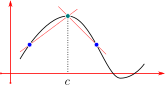
\includegraphics[height=4cm]{extra/loc_max}
 \end{center}
\end{efig}

Consider the derivative of $f'(c)$:
\begin{align*}
f'(c) &= \lim_{h \to 0} \frac{f(c+h)-f(c)}{h}.
\end{align*}
Split the above limit into the left and right limits:
\begin{itemize}
 \item Consider points to the right of $x=c$, For all $h>0$,
\begin{align*}
f(c+h) & \le f(c)  & \text{which implies that} \\
f(c+h)-f(c) &\le 0 & \text{which also implies} \\
\frac{f(c+h)-f(c)}{h} & \le 0 & \text{since
$\frac{\text{negative}}{\text{positive}} = \text{negative}$.}
\end{align*}
But now if we squeeze $h \to 0$ we get
\begin{align*}
  \lim_{h \to 0^+} \frac{f(c+h)-f(c)}{h} &\leq 0
\end{align*}
(provided the limit exists).

\item Consider points to the left of $x=c$. For all $h<0$,
\begin{align*}
f(c+h) & \le f(c)  & \text{which implies that} \\
f(c+h)-f(c) &\le 0 & \text{which also implies} \\
\frac{f(c+h)-f(c)}{h} & \ge 0 & \text{since
$\frac{\text{negative}}{\text{negative}} = \text{positive}$.}
\end{align*}
But now if we squeeze $h \to 0$ we get
\begin{align*}
  \lim_{h \to 0^-} \frac{f(c+h)-f(c)}{h} &\geq 0
\end{align*}
(provided the limit exists).

\item So if the derivative $f'(c)$ exists, then the above right- and left-hand
limits must agree, which forces $f'(c) = 0$.
\end{itemize}
Thus we can conclude that
\begin{quote}
 If the maximum value of $f(x)$ is $f(c)$ and $f'(c)$ exists, then $f'(c)=0$.
\end{quote}
Using similar reasoning one can also see that
\begin{quote}
 If the minimum value of $f(x)$ is $f(c)$ and $f'(c)$ exists, then $f'(c)=0$.
\end{quote}


Notice two things about the above reasoning:
\begin{itemize}
 \item  Firstly, in order for the argument to work we
only need that $f(x)<f(c)$ for $x$ close to $c$ --- it does not matter what happens for
$x$ values far from $c$.
\item Secondly, in the above argument we needed to consider $f(x)$ for $x$ both
to the left of and to the right of $c$. If the function $f(x)$ is defined on a
closed interval $[a,b]$, then the above argument only applies when $a<c<b$ ---
not when $c$ is either of the endpoints $a$ and $b$.

\end{itemize}
Consider the function below
\begin{efig}
 \begin{center}
  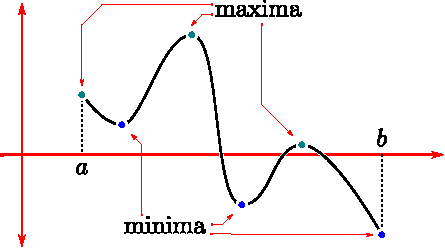
\includegraphics[height=5cm]{extra/maxmin}
 \end{center}
\end{efig}
This function has only 1 maximum value (the middle green point in the graph) and
1 minimum value (the rightmost blue point), however it has 4 points at which the
derivative is zero. In the small intervals around those points where the
derivative is zero, we can see that function is \emph{locally} a maximum or
minimum, even if it is not the \emph{global} maximum or minimum. We clearly need
to be more careful distinguishing between these cases.


\begin{defn}\label{def:APPlocalMaxMin} %%%%%%%%%%%%%%%%%%%%%
Let $a\le b$ and let the function $f(x)$ be defined for all $x \in [a,b]$. Now
let $a \leq c \leq b$, then
\begin{itemize}
\item We say that $f(x)$ has a global (or absolute)
minimum at $x=c$ if $f(x)\ge f(c)$ for all $a\le x\le b$.

\item Similarly, we say that $f(x)$ has a global (or absolute)
maximum at $x=c$ if $f(x)\le f(c)$ for all $a\le x\le b$.

\end{itemize}
Now let $a < c <b$ (note the strict inequalities), then
\begin{itemize}
\item We say that $f(x)$ has a local minimum at $x=c$
if there are $a'$ and $b'$ obeying $a\le a'<c<b'\le b$ such that
$f(x)\ge f(c)$ for all $x$ obeying $a'<x<b'$.  Note the \emph{strict}
inequalities in $a'<c<b'$.

\item Similarly, we say that $f(x)$ has a local maximum at $x=c$
if there are $a'$ and $b'$ obeying $a\le a'<c<b'\le b$ such that
$f(x)\le f(c)$ for all $x$ obeying $a'<x<b'$.  Note the \emph{strict}
inequalities in $a'<c<b'$.
\end{itemize}
The global maxima and minima of a function are called the
global extrema of the function, while the local maxima and minima are called the local
extrema.
\end{defn}

Consider again the function we showed in the figure above
\begin{efig}
 \begin{center}
  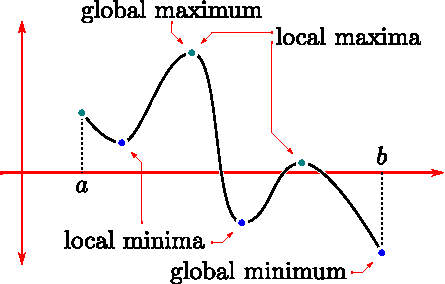
\includegraphics[height=5cm]{extra/maxmin2}
 \end{center}
\end{efig}
It has 2 local maxima and 2 local minima. The global maximum occurs at the middle green
point (which is also a local maximum), while the global minimum occurs at the rightmost
blue point (which is not a local minimum).


Using the above definition we can summarise what we have learned above
as the following theorem\footnote{This is one of several important
mathematical contributions made by Pierre de Fermat, a French government
lawyer and amateur mathematician, who lived in the first half of
the seventeenth century. }:
\begin{theorem}\label{thm:APPlocalMaxMin}
If a function $f(x)$ has a local maximum or local minimum at $x=c$
and if $f'(c)$ exists, then $f'(c)=0$.
\end{theorem}

\begin{itemize}
\item
It is often (but not always) the case that, when $f(x)$ has a local maximum
at $x=c$, the function $f(x)$ increases strictly as $x$ approaches $c$ from the
left and decreases strictly as $x$ leaves $c$ to the right. That is,
$f'(x)>0$ for $x$ just to the left of $c$ and $f'(x)<0$ for $x$ just
to the right of $c$.
Then, it is often the case, because $f'(x)$ is decreasing as $x$ increases through $c$, that $f''(c)<0$.

\item
Conversely, if $f'(c)=0$ and $f''(c)<0$,
  then, just to the right of $c$ $f'(x)$ must be negative, so that
  $f(x)$ is decreasing, and  just to the left of $c$ $f'(x)$ must
  be positive, so that $f(x)$ is increasing.
  So $f(x)$ has a local maximum at $c$.

\item
 Similarly, it is often the case that, when $f(x)$ has a local minimum
 at $x=c$, $f'(x)<0$ for $x$ just to the left of $c$ and $f'(x)>0$ for
 $x$ just to the right of $c$ and $f''(x)>0$.

\item
Conversely, if $f'(c)=0$ and $f''(c)>0$,
  then, just to the right of $c$ $f'(x)$ must be positive, so that
  $f(x)$ is increasing, and, just to the left of $c$ $f'(x)$ must be
  negative, so that $f(x)$ is decreasing.
  So $f(x)$ has a local minimum at $c$.

\end{itemize}


\begin{theorem}\label{thm:APPsecondDerivTest}
If $f'(c)=0$ and $f''(c) <0$, then $f(x)$ has a local maximum at $c$.

If $f'(c)=0$ and $f''(c) >0$, then $f(x)$ has a local minimum at $c$.

\emph{Note the strict inequalities}.

\end{theorem}



Theorem~\ref{thm:APPlocalMaxMin} says that, when $f(x)$ has a local maximum or
minimum at $x=c$, there are two possibilities.
\begin{itemize}
 \item The derivative $f'(c)=0$. This case is illustrated in the following
figure.
\begin{efig}
 \begin{center}
  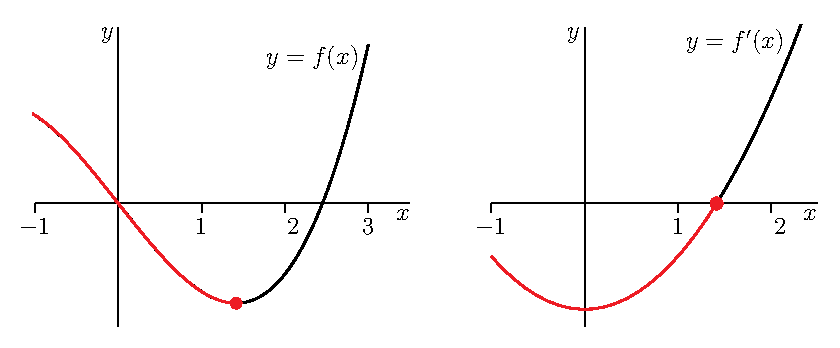
\includegraphics[]{localMaxMinDE}
 \end{center}
\end{efig}
Observe that, in this example, $f'(x)$ changes continuously from negative to
positive at the local minimum, taking the value zero at the local minimum (the
red dot).

\item The derivative $f'(c)$ does not exist. This case is illustrated in the
following figure.
\begin{efig}
 \begin{center}
  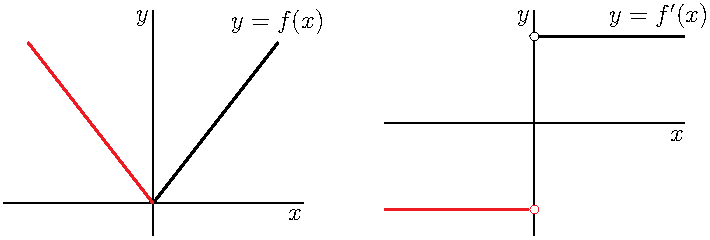
\includegraphics[]{localMaxMinFG}
 \end{center}
\end{efig}
Observe that, in this example, $f'(x)$ changes discontinuously from negative to
positive at the local minimum ($x=0$) and $f'(0)$ does not exist.
\end{itemize}
This theorem demonstrates that the points at which the derivative is zero or
does not exist are very important. It simplifies the discussion that follows if
we give these points names.
\begin{defn}\label{def:APPcriticalPoint} %%%%%%%%%%%%%%%%%%%%%
Let $f(x)$ be a function and let $c$ be a point in its domain. Then
\begin{itemize}
 \item if $f'(c)$ exists and is zero we call $x=c$ a critical point of the
function, and
 \item if $f'(c)$ does not exist then we call $x=c$ a singular point of the
function.
\end{itemize}
\end{defn}

\begin{warning}
Note that some people (and texts) will combine both of these cases and call
$x=c$ a critical point when either the derivative is zero or does not exist.
The reader should be aware of the lack of convention on this point\footnote{No
pun intended.} and should be careful to understand whether the more inclusive
definition of critical point is being used, or if the text is using the more
precise definition that distinguishes critical and singular points.
\end{warning}



We'll now look at a few simple examples involving local maxima and
minima, critical points and singular points. Then we will move on to global
maxima and minima.
\begin{eg}\label{eg:localMinMaxA}
In this example, we'll look for local maxima and minima of the function
$f(x) = x^3-6x$ on the interval $-2\le x\le 3$.
\begin{itemize}
 \item First compute the derivative
\begin{align*}
  f'(x) &= 3x^2-6.
\end{align*}
Since this is a polynomial it is defined everywhere on the domain and so there
will not be any singular points. So we now look for critical points.

 \item To do so we look for zeroes of the derivative
\begin{align*}
  f'(x) &= 3x^2-6 = 3(x^2-2) = 3(x-\sqrt{2})(x+\sqrt{2}).
\end{align*}
This derivative takes the value $0$ at two different values of $x$. Namely
$x=c_-=-\sqrt{2}$ and $x=c_+=\sqrt{2}$. Here is a sketch of the graph of
$f(x)$.
\begin{efig}
\begin{center}
   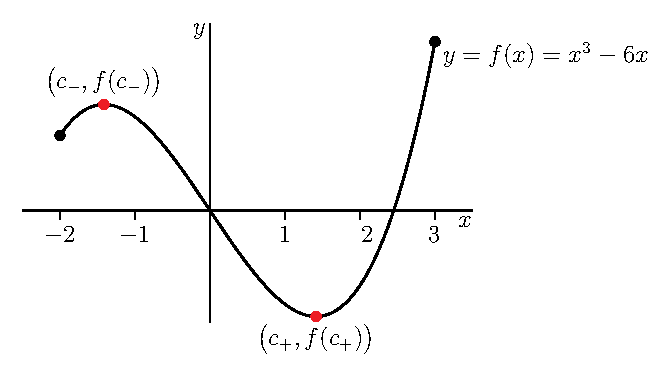
\includegraphics{localMaxMinA}
\end{center}
\end{efig}
From the figure we see that
\begin{itemize}
\item $f(x)$ has a local minimum at $x=c_+$ (i.e. we have $f(x)\ge f(c_+)$
whenever $x$ is close to $c_+$) and
\item $f(x)$ has a local maximum at $x=c_-$ (i.e. we have $f(x)\le f(c_-)$
whenever $x$ is close to $c_-$) and
\item the global minimum of $f(x)$, for $x$ in the interval $-2\le x\le 3$, is
at $x=c_+$ (i.e. we have $f(x)\ge f(c_+)$ whenever $-2\le x\le 3$) and
\item the global maximum of $f(x)$, for $x$ in the interval $-2\le x\le 3$, is
at $x=3$ (i.e. we have $f(x)\le f(3)$ whenever $-2\le x\le 3$).
\end{itemize}
\item Note that we have carefully constructed this example to illustrate that
the global maximum (or minimum) of a function on an interval may or may not also
be a local maximum (or minimum) of the function.
\end{itemize}

\end{eg}

\begin{eg}\label{eg:localMinMaxB}
In this example, we'll look for local maxima and minima of the function
$f(x) = x^3$ on the interval $-1\le x\le 1$.
\begin{itemize}
 \item First compute the derivative:
\begin{align*}
  f'(x) &= 3x^2.
\end{align*}
Again, this is a polynomial and so defined on all of the domain. The function
will not have singular points, but may have critical points.

\item The derivative is zero only when $x=0$, so $x=c=0$ is the only critical
point of the function.
\item The graph of $f(x)$ is sketched below. From that sketch we see that $f(x)$
has \emph{neither} a local maximum \emph{nor} a local minimum at $x=c$ despite
the fact that $f'(c)=0$ --- we have $f(x)<f(c)=0$ for all $x<c=0$ and
$f(x)>f(c)=0$ for all $x>c=0$.
\vadjust{%
\begin{efig}
\begin{center}
   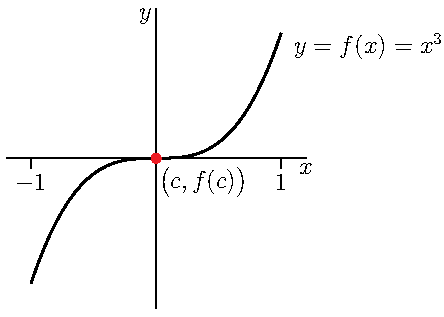
\includegraphics{localMaxMinB}
\end{center}
\end{efig}
}%
\item Note that this example has been constructed to illustrate that a critical
point (or singular point) of a function \emph{need not be a local maximum or
minimum} for the function.
\item Reread Theorem \ref{thm:APPlocalMaxMin}. It says\footnote{A very common
error of logic that people make is ``Affirming the consequent''. ``If P then Q''
is true, then observe Q and conclude P --- this is false. ``If he is Shakespeare then he
is dead'' ``That man is dead'' ``He must be Shakespeare''. Or you may have also seen
someone use this reasoning: ``If a person is a genius before their time then they are
misunderstood.'' ``I am misunderstood'' ``So I must be a genius before my time.''. Or }
that, ``if $f(x)$ has a local maximum/minimum at $x=c$ and if $f$ is differentiable at
$x=c$, then $f'(c)=0$''. It \emph{does not say} that ``if $f'(c)=0$ then $f$
has a local maximum/minimum at $x=c$''.
\end{itemize}
\end{eg}\goodbreak


\begin{eg}\label{eg:localMinMaxC}
In this example, we'll look for local maxima and minima of the function
\begin{align*}
f(x) = |x| = \begin{cases}
           x  & \text{if }x \ge 0 \\
           -x & \text{if }x <  0
       \end{cases}
\end{align*}
on the interval $-1\le x\le 1$.
\begin{itemize}
 \item Again, start by computing the derivative (reread Example~\ref{eg diff
abs}):
\begin{align*}
f'(x) = \begin{cases}
           1  & \text{if }x > 0 \\
           \text{undefined}  & \text{if }x = 0 \\
           -1 & \text{if }x <  0
       \end{cases}
\end{align*}
\item This derivative \emph{never} takes the value $0$, so the function does
not have any critical points. However the derivative does not exist at the
point $x=0$, so that point is a singular point.

\item Here is a sketch of the graph of $f(x)$.
\begin{efig}
\begin{center}
   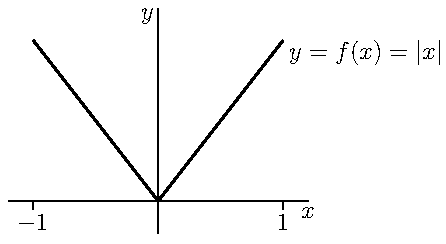
\includegraphics{localMaxMinC}
\end{center}
\end{efig}
From the figure we see that $f(x)$ has a local (and in fact global)
minimum at $x=0$ despite the fact that $f'(0)$ is not a critical point.
\item Reread Theorem \ref{thm:APPlocalMaxMin} yet again. It says that,
``if $f(x)$ has a local maximum/minimum at $x=c$
\emph{and if $f$ is differentiable at $x=c$}, then $f'(c)=0$''.
It says nothing about what happens at points where the derivative does
not exist. Indeed that is why we have to consider both critical points and
singular points when we look for maxima and minima.
\end{itemize}
\end{eg}




\subsection{Finding Global Maxima and Minima}\label{ssec find maxmin}
We now have a technique for finding local maxima and minima --- just look
for values of $x$ for which either $f'(x)=0$ or $f'(x)$ does not exist.
What about finding global maxima and minima? We'll start by stating
explicitly that, under appropriate hypotheses, global maxima
and minima are guaranteed to exist.
\begin{theorem}\label{thm:APPglobalMaxMinExist}
Let the function $f(x)$ be defined and continuous on the closed,
finite interval\footnote{The hypotheses that $f(x)$ be continuous
and that the interval be finite and closed are all essential.
We suggest that you find three functions $f_1(x)$, $f_2(x)$ and
$f_3(x)$ with $f_1$ defined but not continuous on $0\le x\le 1$,
$f_2$ defined and continuous on $-\infty<x<\infty$, and $f_3$ defined
and continuous on $0<x<1$, and with none of $f_1$, $f_2$ and $f_3$
attaining either a global maximum or a global minimum.}
$-\infty<a\le x\le b<\infty$. Then $f(x)$ attains
a maximum and a minimum at least once. That is, there exist
numbers $a\le x_m, x_M\le b$ such that
\begin{align*}
f(x_m)\le f(x)\le f(x_M)
\qquad\text{for all }a\le x\le b
\end{align*}
\end{theorem}
So let's again consider the
question
\begin{quote}
Suppose that the maximum (or minimum) value of $f(x)$, for $a\le x\le b$, is $f(c)$.
What does that tell us about $c$?
\end{quote}
If $c$ obeys $a<c<b$ (note the strict inequalities), then $f$ has
a local maximum (or minimum) at $x=c$ and Theorem  \ref{thm:APPlocalMaxMin}
tells us that either $f'(c)=0$ or $f'(c)$ does not exist. The only other place that a
maximum or minimum can occur are at the ends of the interval. We can summarise this as:
\begin{theorem}\label{thm:APPglobalMaxMin}
If $f(x)$ has a global maximum or global minimum, for $a\le x\le b$,
at $x=c$ then there are 3 possibilities. Either
\begin{itemize}
\item $f'(c)=0$, or
\item $f'(c)$ does not exist, or
\item $c=a$ or $c=b$.
\end{itemize}
That is, a global maximum or minimum must occur either at a critical point, a singular
point or at the endpoints of the interval.
\end{theorem}

This theorem provides the basis for a method to find the maximum and
minimum values of $f(x)$ for $a\le x\le b$:
\begin{cor}\label{cor find maxmin}
 Let $f(x)$ be a function on the interval $a \leq x \leq b$. Then to find the global
maximum and minimum of the function:
\begin{itemize}
\item Make a list of all values of $c$, with $a\le c\le b$, for which
      \begin{itemize}
          \item $f'(c)=0$, or
          \item $f'(c)$ does not exist, or
          \item $c=a$ or $c=b$.
      \end{itemize}
  That is --- compute the function at all the critical points, singular points, and
endpoints.

\item Evaluate $f(c)$ for each $c$ in that list. The largest (or smallest)
      of those values is the largest (or smallest) value of $f(x)$
      for $a\le x\le b$.
\end{itemize}
\end{cor}
Let's now demonstrate how to use this strategy. The function in  this first example is
not too simple --- but it is a good example of a function that contains both a
singular point and a critical point.
\begin{eg}\label{APPglobalMaxMinA}
Find the largest and smallest values of the function $f(x)=2x^{5/3}+3x^{2/3}$ for $-1\le
x\le 1$.

\soln We will apply the method in Corollary~\ref{cor find maxmin}. It is perhaps easiest
to find the values at the endpoints of the intervals and then move on to the values at
any critical or singular points.
\begin{itemize}
 \item Before we get into things, notice that we can rewrite the function by factoring
it:
\begin{align*}
  f(x) &= 2x^{5/3}+3x^{2/3} = x^{2/3} \cdot \left(2x + 3\right)
\end{align*}
 \item Let's compute the function at the endpoints of the interval:
\begin{align*}
  f(1) &= 2 +3 = 5 \\
  f(-1) &= 2 \cdot(-1)^{5/3} + 3\cdot (-1)^{2/3} =-2 + 3 = 1
\end{align*}
\item To compute the function at the critical and singular points we first need to find
the derivative:
\begin{align*}
  f'(x) &= 2 \cdot \frac{5}{3} x^{2/3} + 3 \cdot \frac{2}{3} x^{-1/3} \\
  &= \frac{10}{3} x^{2/3} + 2 x^{-1/3}\\
  &= \frac{10 x + 6}{3 x^{1/3}}
\end{align*}
\item Notice that the numerator and denominator are defined for all $x$. The only place
the derivative is undefined is when the denominator is zero. Hence the only singular
point is at $x=0$. The corresponding function value is
\begin{align*}
  f(0) &= 0
\end{align*}
\item To find the critical points we need to solve $f'(x) = 0$:
\begin{align*}
  0 &= \frac{10 x + 6}{3 x^{1/3}}
\end{align*}
Hence we must have $10x=-6$ or $x=-3/5$. The corresponding function value is
\begin{align*}
  f(x) &= x^{2/3} \cdot \left(2x + 3\right) & \text{recall this from above, then}\\
  f(-3/5) &= (-3/5)^{2/3} \cdot\left(2 \cdot \frac{-3}{5} + 3 \right) \\
  &= \left(\frac{9}{25}\right)^{1/3} \cdot \frac{-6 + 15}{5} \\
  &= \left(\frac{9}{25}\right)^{1/3} \cdot \frac{9}{5}  \approx 1.28
\end{align*}
Note that if we do not want to approximate the root (if, for example, we do not have a
calculator handy), then we can also write
\begin{align*}
  f(-3/5) &= \left(\frac{9}{25}\right)^{1/3} \cdot \frac{9}{5} \\
  &= \left(\frac{9}{25}\right)^{1/3} \cdot \frac{9}{25} \cdot 5 \\
  &= 5 \cdot \left( \frac{9}{25} \right)^{4/3}
\end{align*}
Since $0<9/25<1$, we know that $0 < \left( \frac{9}{25} \right)^{4/3} < 1$, and hence
\begin{align*}
  0 < f(-3/5) = 5 \cdot \left( \frac{9}{25} \right)^{4/3} < 5.
\end{align*}

\item We summarise our work in this table
\begin{center}
\begin{tabular}{|c||c|c|c|c|}
\hline
$c$ & $-\frac{3}{5}$ &  $0$ &  $-1$ & $1$ \\
\hline
type & critical point & singular point & endpoint & endpoint \\
\hline
$f(c)$ & $\frac{9}{5}\root{3}\of{\frac{9}{25}}\approx 1.28$ & $0$ & $1$ & $5$\\
\hline
\end{tabular}
\end{center}
\item The largest value of $f$ in the table is $5$ and the smallest value of $f$ in the
table is $0$.
\item Thus on the interval $-1\leq x \leq 1$ the global maximum of $f$ is $5$, and is
taken at $x=1$, while the global minimum value of $f(x)$ is $0$, and is taken at $x=0$.

\item For completeness we also sketch the graph of this function on the same interval.
\begin{efig}
\begin{center}
   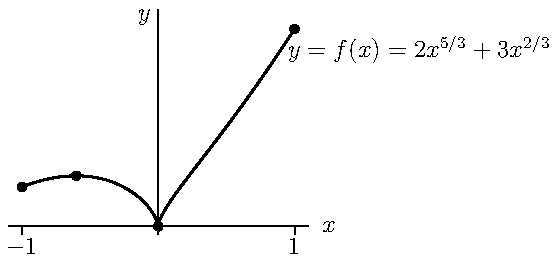
\includegraphics{globalMaxMinA}
\end{center}
\end{efig}
Later (in Section~\ref{sec curve sketch}) we will see how to construct such a sketch
without using a calculator or computer.
\end{itemize}
\end{eg}


\subsection{Max/Min Examples}\label{sec opt eg}
As noted at the beginning of this section, the problem of finding maxima and minima is
a very important application of differential calculus in the real world. We now turn to a
number of examples of this process. But to guide the reader we will describe a general
procedure to follow for these problems.

\begin{enumerate}[(1)]
 \item Read --- read the problem carefully. Work out what information is given in the
statement of the problem and what we are being asked to compute.
\item Diagram --- draw a diagram. This will typically help you to identify what you know
about the problem and what quantities you need to work out.
\item Variables --- assign variables to the quantities in the problem along
with their units. It is typically a good idea to make sensible choices of variable names:
$A$ for area, $h$ for height, $t$ for time etc.
\item Relations --- find relations between the variables. By now you should know the
quantity we are interested in (the one we want to maximise or minimise) and we
need to establish a relation between it and the other variables.
\item Reduce --- the relation down to a function of one variable. In order to apply the
calculus we know, we must have a function of a single variable. To do this we need to use
all the information we have to eliminate variables. We should also work out
the domain of the resulting function.
\item Maximise or minimise --- we can now apply the methods of Corollary~\ref{cor find
maxmin} to find the maximum or minimum of the quantity we need (as the problem dictates).
\item Be careful --- make sure your answer makes sense. Make sure quantities are
physical. For example, lengths and areas cannot be negative.
\item Answer the question --- be sure your answer really answers the question asked in
the problem.
\end{enumerate}

Let us start with a relatively simple problem:
\begin{eg}\label{APPglobalMaxMinB}
A closed rectangular container with a square base is to be made
from two different materials. The material for the base costs \$5 per square
meter, while the material for the other five sides costs \$1 per square
meter. Find the dimensions of the container which has the largest possible
volume if the total cost of materials is \$72.

\soln We can follow the steps we outlined above to find the solution.
\begin{itemize}
 \item We need to determine the area of the two types of materials used and the
corresponding total cost.
 \item Draw a picture of the box.
\begin{efig}
\centering
 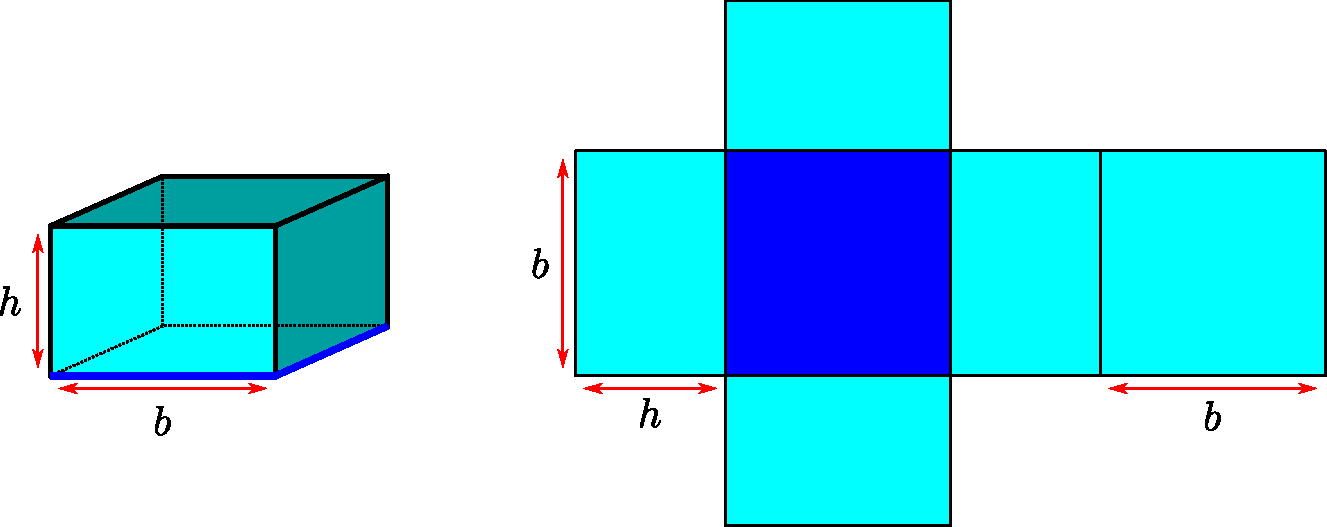
\includegraphics[height=5cm]{extra/container}
\end{efig}
The more useful picture is the unfolded box on the right.
\item In the picture we have already introduced two variables. The square base has
side-length $b$ metres and it has height $h$ metres. Let the area of the base be $A_b$
and the area of the other fives sides be $A_s$ (both in $m^2$), and the total cost be
$C$ (in dollars). Finally let the volume enclosed be $V m^3$.
\item Some simple geometry tells us that
\begin{align*}
  A_b &= b^2 \\
  A_s &= 4 bh + b^2 \\
  V &= b^2h\\
  C &= 5 \cdot A_b + 1\cdot A_s = 5b^2+4bh+b^2 = 6b^2+4bh.\\
\end{align*}
\item To eliminate one of the variables we use the fact that the total cost is \$72.
\begin{align*}
  C &= 6b^2+4bh = 72 & \text{rearrange}\\
  4bh &= 72-6b^2  & \text{isolate $h$}\\
  h &= \frac{72-6b^2}{4b} = \frac{3}{2} \cdot \frac{12-b^2}{b}
\end{align*}
Substituting this into the volume gives
\begin{align*}
  V&= b^2 h = \frac{3b}{2} (12-b^2) = 18b - \frac{3}{2} b^3
\end{align*}
Now note that since $b$ is a length it cannot be negative, so $b \geq 0$. Further since
volume cannot be negative, we must also have
\begin{align*}
  12-b^2 \geq 0
\end{align*}
and so $b \leq \sqrt{12}$.

\item Now we can apply Corollary~\ref{cor find maxmin} on the above expression for
the volume with $0 \leq b \leq \sqrt{12}$. The endpoints give:
\begin{align*}
  V(0) &= 0 \\
  V(\sqrt{12}) &= 0
\end{align*}
The derivative is
\begin{align*}
  V'(b) &= 18 - \frac{9b^2}{2}
\end{align*}
Since this is a polynomial there are no singular points. However we can solve $V'(b) = 0$
to find critical points:
\begin{align*}
  18 - \frac{9b^2}{2} &= 0  & \text{divide by 9 and multiply by 2}\\
  4 - b^2 &= 0
\end{align*}
Hence $b = \pm 2$. Thus the only critical point in the domain is $b=2$. The corresponding
volume is
\begin{align*}
V(2) &= 18\times2 - \frac{3}{2} \times 2^3 \\
  &= 36 - 12 = 24.
\end{align*}
So by Corollary~\ref{cor find maxmin}, the maximum volume is when 24 when $b=2$ and
\begin{align*}
  h &= \frac{3}{2} \cdot \frac{12-b^2}{b} = \frac{3}{2} \frac{12-4}{2} = 6.
\end{align*}
\item All our quantities make sense; lengths, areas and volumes are all non-negative.
\item Checking the question again, we see that we are asked for the dimensions of the
container (rather than its volume) so we can answer with
\begin{quote}
 The container with dimensions $2 \times 2 \times 6m$ will be the largest possible.
\end{quote}
\end{itemize}
\end{eg}


\begin{eg}\label{APPglobalMaxMinC}
A rectangular sheet of cardboard is 6 inches by 9 inches. Four
identical squares are cut from the corners of the cardboard, as shown in
the figure below, and the remaining piece is folded into an open
rectangular box. What should the size of the cut out squares be in
order to maximize the volume of the box?

\soln This one is quite similar to the previous one, so we perhaps don't need to go into
so much detail.
\begin{itemize}
 \item After reading carefully we produce the following picture:
\begin{efig}
\begin{center}
   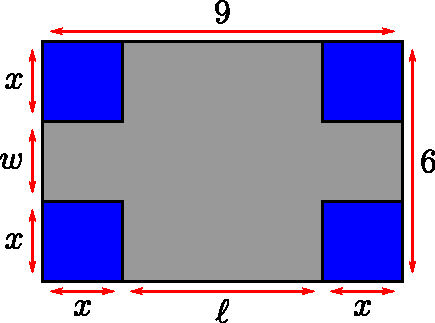
\includegraphics[height=5cm]{extra/box_vol}
\end{center}
\end{efig}

\item Let the height of the box be $x$ inches, and the base be $\ell \times w$ inches.
The volume of the box is then $V$ cubic inches.
\item Some simple geometry tells us that $\ell = 9-2x, w=6-2x$ and so
\begin{align*}
V &= x(9-2x)(6-2x) \text{cubic inches}\\
  &= 54x-30x^2+4x^3.
\end{align*}
Notice that since all lengths must be non-negative, we must have
\begin{align*}
  x,\ell,w \geq 0
\end{align*}
and so $0 \leq x \leq 3$ (if $x>3$ then $w<0$).
\item We can now apply Corollary~\ref{cor find maxmin}. First the endpoints of the
interval give
\begin{align*}
  V(0) &= 0 & V(3) &= 0
\end{align*}
The derivative is
\begin{align*}
  V'(x) &= 54 - 60x +12x^2 \\
  &= 6(9-10x+2x^2)
\end{align*}
Since this is a polynomial there are no singular points. To find critical points we solve
$V'(x) = 0$ to get
\begin{align*}
  x_\pm &= \frac{10 \pm \sqrt{100 - 4\times2\times9}}{4} \\
  &= \frac{10 \pm \sqrt{28}}{4} = \frac{10 \pm 2\sqrt{7}}{4} = \frac{5 \pm \sqrt{7}}{2}
\end{align*}
We can then use a calculator to approximate
\begin{align*}
  x_+ &\approx 3.82 & x_- &\approx 1.18.
\end{align*}
So $x_-$ is inside the domain, while $x_+$ lies outside.

Alternatively\footnote{Say if we do not have a calculator to hand, or your instructor
insists that the problem be done without one.}, we can bound $x_\pm$ by first noting that
$2 \leq \sqrt{7} \leq 3$. From this we know that
\begin{align*}
  1=\frac{5-3}{2} & \leq x_- = \frac{5 - \sqrt{7}}{2} \leq \frac{5-2}{2} = 1.5 \\
  3.5=\frac{5+2}{2} & \leq x_+ = \frac{5 + \sqrt{7}}{2} \leq \frac{5+3}{2} = 4
\end{align*}

\item Since the volume is zero when $x=0,3$, it must be the case that the volume is
maximised when $x = x_- = \frac{5 - \sqrt{7}}{2}$.

\item Notice that since $0 < x_- <3$ we know that the other lengths are positive, so our
answer makes sense. Further, the question only asks for the length $x$ and not the
resulting volume so we have answered the question.
\end{itemize}
\end{eg}

There is a new wrinkle in the next two examples. Each involves finding the
minimum value of a function $f(x)$ with $x$ running over all real numbers,
rather than just over a finite interval as in Corollary~\ref{cor find maxmin}.
Both in Example~\ref{APPglobalMaxMinD} and in Example~\ref{APPglobalMaxMinDist}
the function $f(x)$ tends to $+\infty$ as $x$ tends to either $+\infty$ or
$-\infty$. So the minimum value of $f(x)$ will be achieved for some finite value
of $x$, which will be a local minimum as well as a global minimum.

\begin{theorem}\label{thm:maxMinOnR}
Let $f(x)$ be defined and continuous for all $-\infty<x<\infty$. Let $c$ be a finite
real number.

\begin{enumerate}[(a)]
\item If $\displaystyle \lim_{x\rightarrow+\infty} f(x)=+\infty$ and
$\displaystyle \lim_{x\rightarrow-\infty} f(x)=+\infty$ and if $f(x)$ has a global
minimum at $x = c$, then there are 2 possibilities. Either
  \begin{itemize}
  \item  $f'(c) = 0$, or
  \item  $f'(c)$ does not exist
  \end{itemize}
That is, a global minimum must occur either at a critical point or at a singular point.

\item If $\displaystyle \lim_{x\rightarrow+\infty} f(x)=-\infty$ and
$\displaystyle \lim_{x\rightarrow-\infty} f(x)=-\infty$ and if $f(x)$ has a global
maximum at $x = c$, then there are 2 possibilities. Either
\begin{itemize}
  \item  $f'(c) = 0$, or
  \item  $f'(c)$ does not exist
\end{itemize}
That is, a global maximum must occur either at a critical point or at a singular point.
\end{enumerate}
\end{theorem}


\begin{eg}\label{APPglobalMaxMinD}
Find the point on the line $y=6-3x$ that is closest to the point $(7,5)$.

\soln In this problem

\begin{itemize}
 \item A simple picture
\begin{efig}
 \begin{center}
  \includegraphics[height=55mm]{extra/line_dist}
 \end{center}
\end{efig}
  \item Some notation is already given to us. Let a point on the line have coordinates
$(x,y)$, and we do not need units. And let $\ell$ be the distance from the point $(x,y)$
to the point~$(7,5)$.
\item Since the points are on the line the coordinates $(x,y)$ must obey
\begin{align*}
  y=6-3x
\end{align*}
Notice that $x$ and $y$ have no further constraints. The distance $\ell$ is given by
\begin{align*}
  \ell^2 &= (x-7)^2 + (y-5)^2
\end{align*}
\item We can now eliminate the variable $y$:
\begin{align*}
  \ell^2 &= (x-7)^2 + (y-5)^2 \\
  &= (x-7)^2 + (6-3x-5)^2 = (x-7)^2 + (1-3x)^2 \\
  &= x^2-14x+49 + 1-6x+9x^2 = 10x^2-20x+50 \\
  &= 10(x^2-2x+5) \\
  \ell &= \sqrt{10} \cdot \sqrt{x^2-2x+5}
\end{align*}
Notice that as $x \to \pm \infty$ the distance $\ell \to +\infty$.

\item We can now apply Theorem~\ref{thm:maxMinOnR}
\begin{itemize}
 \item Since the distance is defined for all real $x$, we do not have to check the
endpoints of the domain --- there are none.
\item Form the derivative:
\begin{align*}
  \diff{\ell}{x} &= \sqrt{10} \frac{2x-2}{2\sqrt{x^2-2x+5}}
\end{align*}
It is zero when $x=1$, and undefined if $x^2-2x+5<0$. However, since
\begin{align*}
  x^2-2x+5 &= (x^2-2x+1)+4 = \underbrace{(x-1)^2}_{\geq0}+4
\end{align*}
we know that $x^2-2x+5 \geq 4$. Thus the function has no singular points and the only
critical point occurs at $x=1$. The corresponding function value is then
\begin{align*}
  \ell(1) &=\sqrt{10} \sqrt{1-2+5} = 2 \sqrt{10}.
\end{align*}
\item Thus the minimum value of the distance is $\ell=2 \sqrt{10}$ and occurs at $x=1$.
\end{itemize}
\item This answer makes sense --- the distance is not negative.
\item The question asks for the point that minimises the distance, not that minimum
distance. Hence the answer is $x=1, y=6-3 = 3$. I.e.
\begin{quote}
 The point that minimises the distance is $(1,3)$.
\end{quote}
\end{itemize}

Notice that we can make the analysis easier by observing that the point that minimises
the distance also minimises the squared-distance. So that instead of minimising the
function $\ell$, we can just minimise $\ell^2$:
\begin{align*}
  \ell^2 &= 10(x^2-2x+5)
\end{align*}
The resulting algebra is a bit easier and we don't have to hunt for singular points.

\end{eg}

\begin{eg}\label{APPglobalMaxMinDist}
 Find the minimum distance from $(2,0)$ to the curve $y^2=x^2+1$.

\soln This is very much like the previous question.
\begin{itemize}
 \item After reading the problem carefully we can draw a picture
\begin{efig}
\begin{center}
   \includegraphics{hyperbolaMaxMin}
\end{center}
\end{efig}
\item In this problem we do not need units and the variables $x,y$ are supplied. We define
the distance to be $\ell$ and it is given by
\begin{align*}
  \ell^2 &= (x-2)^2+y^2.
\end{align*}
As noted in the previous problem, we will minimise the squared-distance since that also
minimises the distance.
\item Since $x,y$ satisfy $y^2=x^2+1$, we can write the distance as a function of $x$:
\begin{align*}
  \ell^2 &= (x-2)^2 + y^2 = (x-2)^2 + (x^2+1)\\
\end{align*}
Notice that as $x \to \pm \infty$ the squared-distance $\ell^2 \to +\infty$.

\item Since the squared-distance is a polynomial it will not have any singular points,
only critical points. The derivative is
\begin{align*}
  \diff{}{x} \ell^2 &= 2(x-2) + 2x = 4x-4
\end{align*}
so the only critical point occurs at $x=1$.

\item When $x=1, y=\pm \sqrt{2}$ and the distance is
\begin{align*}
  \ell^2 &= (1-2)^2 + (1+1) = 3 & \ell=\sqrt{3}
\end{align*}
and thus the minimum distance from the curve to $(2,0)$ is $\sqrt{3}$.
\end{itemize}
\end{eg}

\begin{eg}\label{APPglobalMaxMinrain}
A water trough is to be constructed from a metal sheet of width $45$ cm
by bending up one third of the sheet on each side through an angle
$\theta$.  Which $\theta$ will allow the trough to carry the maximum
amount of water?


\soln Clearly $0 \leq \theta \leq \pi$, so we are back in the domain\footnote{Again, no
pun intended.} of Corollary~\ref{cor find maxmin}.
\begin{itemize}
 \item After reading the problem carefully we should realise that it is really asking us
to maximise the cross-sectional area. A figure really helps.

\begin{efig}
\begin{center}
   \includegraphics{extra/gutter}
\end{center}
\end{efig}

\item From this we are led to define the height $h$ $cm$ and cross-sectional area $A$
$cm^2$. Both are functions of $\theta$.
\begin{align*}
  h &= 15 \sin \theta
\end{align*}
while the area can be computed as the sum of the central $15 \times h$ rectangle, plus
two triangles. Each triangle has height $h$ and base $15 \cos \theta$. Hence
\begin{align*}
  A &= 15h + 2 \cdot \frac{1}{2} \cdot h \cdot 15 \cos \theta \\
  &= 15h \left(1 + \cos \theta \right)
\end{align*}
\item Since $h = 15\sin \theta$ we can rewrite the area as a function of just $\theta$:
\begin{align*}
  A(\theta) &= 225 \sin\theta \left(1 + \cos \theta \right)
\end{align*}
where $0 \leq \theta \leq \pi$.

\item Now we use Corollary~\ref{cor find maxmin}. The ends of the interval give
\begin{align*}
  A(0) &= 225 \sin 0 (1 + \cos 0) = 0 \\
  A(\pi) &= 225 \sin \pi ( 1+ \cos \pi) = 0
\end{align*}
The derivative is
\begin{align*}
  A'(\theta) &= 225 \cos\theta \cdot (1+\cos\theta) + 225 \sin\theta \cdot(-\sin\theta) \\
  &= 225 \left[ \cos \theta + \cos^2\theta - \sin^2\theta \right]
&\text {recall $\sin^2\theta = 1 - \cos^2\theta$}\\
  &= 225 \left[ \cos\theta +2\cos^2\theta -1 \right]
\end{align*}
This is a continuous function, so there are no singular points. However we can still hunt
for critical points by solving $A'(\theta) = 0$. That is
\begin{align*}
  2\cos^2\theta + \cos \theta -1 &= 0 & \text{factor carefully}\\
  (2\cos\theta -1)(\cos \theta+1) &= 0
\end{align*}
Hence we must have $\cos \theta =-1$ or $\cos\theta = \half$. On the domain $0\leq \theta
\leq \pi$, this means $\theta = \pi/3$ or $\theta = \pi$.
\begin{align*}
  A(\pi) &= 0 \\
  A(\pi/3) &= 225 \sin(\pi/3) (1 + \cos(\pi/3)) \\
  & = 225 \cdot \frac{\sqrt{3}}{2} \cdot \left( 1 + \frac{1}{2} \right) \\
  &= 225 \cdot \frac{3\sqrt{3}}{4} \approx 292.28
\end{align*}
\item Thus the cross-sectional area is maximised when $\theta = \dfrac{\pi}{3}$.
\end{itemize}
\end{eg}


\begin{eg}\label{APPglobalMaxMinDD}
Find the points on the ellipse $\frac{x^2}{4}+y^2=1$ that are nearest
to and farthest from the point $(1,0)$.


\soln While this is another distance problem, the possible values of $x,y$ are bounded,
so we need Corollary~\ref{cor find maxmin} rather than Theorem~\ref{thm:maxMinOnR}.
\begin{itemize}
 \item We start by drawing a picture:
\begin{efig}
\begin{center}
   \includegraphics{ellipseMaxMin}
\end{center}
\end{efig}
\item Let $\ell$ be the distance from the point $(x,y)$ on the ellipse to the point
$(1,0)$. As was the case above, we will maximise the squared-distance.
\begin{align*}
  \ell^2 &= (x-1)^2 + y^2.
\end{align*}
\item Since $(x,y)$ lie on the ellipse we have
\begin{align*}
\frac{x^2}{4}+y^2=1
\end{align*}
Note that this also shows that $-2 \leq x \leq 2$ and $-1 \leq y \leq 1$.


Isolating $y^2$ and substituting this into our expression for $\ell^2$ gives
\begin{align*}
  \ell^2 &= (x-1)^2 + \underbrace{1-x^2/4}_{=y^2}.
\end{align*}

\item Now we can apply Corollary~\ref{cor find maxmin}. The endpoints of the domain give
\begin{align*}
  \ell^2(-2) &= (-2-1)^2 + 1 - (-2)^2/4 = 3^2+1-1 = 9\\
  \ell^2(2) &= (2-1)^2 + 1 - 2^2/4 = 1+1-1 = 1
\end{align*}
The derivative is
\begin{align*}
  \diff{}{x} \ell^2 &= 2(x-1) - x/2 = \frac{3x}{2} - 2
\end{align*}
Thus there are no singular points, but there is a critical point at $x = 4/3$. The
corresponding squared-distance is
\begin{align*}
  \ell^2(4/3) &= \left( \frac{4}{3}-1\right)^2 +1 - \frac{(4/3)^2}{4} \\
  &= (1/3)^2 + 1 - (4/9) = 6/9 = 2/3.
\end{align*}

\item To summarise (and giving distances and coordinates of points):
\begin{center}
           \renewcommand{\arraystretch}{1.5}
     \begin{tabular}{|c|c|c|}
          \hline
                  $x$ &  $(x,y)$ &  $\ell$
           \\ \hline
               $-2$ & $(-2,0)$ & $3$
           \\ \hline
               $\nicefrac{4}{3}$
                   & $\big(\nicefrac{4}{3},\pm\nicefrac{\sqrt{5}}{3}\big)$
                   & $\sqrt{\nicefrac{2}{3}}$
           \\ \hline
               $2$ & $(2,0)$ & $1$
           \\ \hline
     \end{tabular}
           \renewcommand{\arraystretch}{1}
\end{center}
The point of maximum distance is $(-2,0)$, and the point of minimum distance is
$\left(\nicefrac{4}{3},\pm\nicefrac{\sqrt{5}}{3}\right)$.
\end{itemize}

\end{eg}


\begin{eg}\label{APPglobalMaxMinE}
Find the dimensions of the rectangle of largest area that can be inscribed in an
equilateral triangle of side $a$ if one side of the rectangle lies on the base
of the triangle.

\soln Since the rectangle must sit inside the triangle, its dimensions are
bounded and we will end up using Corollary~\ref{cor find maxmin}.
\begin{itemize}
 \item Carefully draw a picture:
\begin{efig}
\begin{center}
   \includegraphics{inscribedB}
  \quad
   \includegraphics{inscribed}
\end{center}
\end{efig}
We have drawn (on the left) the triangle in the $xy$-plane with its base on the
$x$-axis. The base has been drawn running from $(-a/2,0)$ to $(a/2,0)$ so
its centre lies at the origin. A little Pythagoras (or a little trigonometry)
tells us that the height of the triangle is
\begin{align*}
  \sqrt{a^2-(a/2)^2} &= \frac{\sqrt{3}}{2}\cdot a = a\cdot \sin\frac{\pi}{3}
\end{align*}
Thus the vertex at the top of the triangle lies at
$\left(0,\frac{\sqrt{3}}{2}\cdot a\right)$.

\item If we construct a rectangle that does not touch the sides of the
triangle, then we can increase the dimensions of the rectangle until it touches
the triangle and so make its area larger. Thus we can assume that the
two top corners of the rectangle touch the triangle as drawn in the
right-hand figure above.

\item Now let the rectangle be $2x$ wide and $y$ high. And let $A$ denote its
area. Clearly
\begin{align*}
  A &= 2xy.
\end{align*}
where $0 \leq x \leq a/2$ and $0\leq y\leq \frac{\sqrt{3}}{2}a$.


\item Our construction means that the top-right corner of the rectangle will
have coordinates $(x,y)$ and lie on the line joining the top vertex of the
triangle at $(0,\sqrt{3}a/2)$ to the bottom-right vertex at $(a/2,0)$. In order
to write the area as a function of $x$ alone, we need the equation for this
line since it will tell us how to write $y$ as a function of $x$. The line has
slope
\begin{align*}
  \text{slope} &= \frac{\sqrt{3}a/2 - 0}{0-a/2} = -\sqrt{3}.
\end{align*}
and passes through the point $(0,\sqrt{3}a/2)$, so any point $(x,y)$ on that
line satisfies:
\begin{align*}
  y &= -\sqrt{3}x + \frac{\sqrt{3}}{2}a.
\end{align*}
\item We can now write the area as a function of $x$ alone
\begin{align*}
  A(x) &= 2x \left( -\sqrt{3}x + \frac{\sqrt{3}}{2}a \right)\\
  &= \sqrt{3} x(a-2x).
\end{align*}
with $0\leq x \leq a/2$.
\item The ends of the domain give:
\begin{align*}
  A(0) &= 0 & A(a/2) &= 0.
\end{align*}
The derivative is
\begin{align*}
  A'(x) &= \sqrt{3} \left( x \cdot (-2) + 1 \cdot (a-2x) \right) = \sqrt{3}
(a-4x).
\end{align*}
Since this is a polynomial there are no singular points, but there is a
critical point at $x=a/4$. There
\begin{align*}
  A(a/4) &= \sqrt{3} \cdot \frac{a}{4} \cdot (a - a/2) = \sqrt{3} \cdot
\frac{a^2}{8}. \\
  y &= -\sqrt{3}\cdot (a/4) + \frac{\sqrt{3}}{2} a = \sqrt{3}\cdot \frac{a}{4}.
\end{align*}
\item Checking the question again, we see that we are asked for the dimensions
rather than the area, so the answer is $2x \times y$:
\begin{quote}
 The largest such rectangle has dimensions $\frac{a}{2} \times \frac{\sqrt{3}
a}{4}$.
\end{quote}

\end{itemize}

\end{eg}


This next one is a good physics example. In it we will derive Snell's
Law\footnote{Snell's law is named after the Dutch astronomer Willebrord Snellius
who derived it in around 1621, though it was first stated accurately in 984 by
Ibn Sahl.} from Fermat's principle\footnote{Named after Pierre de Fermat who
described it in a letter in 1662. The beginnings of the idea, however, go back
as far as Hero of Alexandria in around 60CE. Hero is credited with many
inventions including the first vending machine, and a precursor of the steam
engine called an aeolipile.}.
\begin{eg}\label{APPglobalMaxMinF}
Consider the figure below which shows the trajectory of a ray of light as it
passes through two different mediums (say air and water).
\begin{efig}
\begin{center}
   \includegraphics{snell}
\end{center}
\end{efig}
Let $c_a$ be the speed of light in air and $c_w$ be the speed of
light in water. Fermat's principle states that a ray of light will always
travel along a path that minimises the time taken. So if a ray of light travels
from $P$ (in air) to $Q$ (in water) then it will ``choose'' the point $O$ (on
the interface) so as to minimise the total time taken. Use this idea to show
Snell's law,
\begin{align*}
  \frac{\sin\theta_i}{\sin\theta_r}&=\frac{c_a}{c_w}
\end{align*}
where $\theta_i$ is the angle of incidence and $\theta_r$ is the angle
of refraction (as illustrated in the figure above).


\soln This problem is a little more abstract than the others we have examined,
but we can still apply Theorem~\ref{thm:maxMinOnR}.
\begin{itemize}
 \item We are given a figure in the statement of the problem and it contains
all the relevant points and angles. However it will simplify things if we
decide on a coordinate system. Let's assume that the point $O$ lies on the
$x$-axis, at coordinates $(x,0)$. The point $P$ then lies above the axis at
$(X_P,+Y_P)$, while $Q$ lies below the axis at $(X_Q,-Y_Q)$. This is drawn below.
\begin{efig}
\begin{center}
   \includegraphics{snellB}
\end{center}
\end{efig}



\item The statement of Snell's law contains terms $\sin \theta_i$ and $\sin
\theta_r$, so it is a good idea for us to see how to express these in terms of
the coordinates we have just introduced:
\begin{align*}
  \sin \theta_i &=  \frac{\text{opposite}}{\text{hypotenuse}}
  = \frac{(x-X_P)}{\sqrt{(X_P-x)^2 + Y_P^2}}\\
  \sin \theta_r &=  \frac{\text{opposite}}{\text{hypotenuse}}
  = \frac{(X_Q-x)}{\sqrt{(X_Q-x)^2 + Y_Q^2}}
\end{align*}

\item Let $\ell_P$ denote the distance $PO$, and $\ell_Q$ denote the distance
$OQ$. Then we have
\begin{align*}
  \ell_P &= \sqrt{(X_P-x)^2+Y_P^2} \\
  \ell_Q &= \sqrt{(X_Q-x)^2+Y_Q^2}
\end{align*}
If we then denote the total time taken by $T$, then
\begin{align*}
  T &= \frac{\ell_P}{c_a} + \frac{\ell_Q}{c_w}
  = \frac{1}{c_a}\sqrt{(X_P-x)^2+Y_P^2} + \frac{1}{c_w}\sqrt{(X_Q-x)^2+Y_Q^2}
\end{align*}
which is written as a function of $x$ since all the other terms are
constants.

\item Notice that as $x \to +\infty$ or $x\to-\infty$ the total time $T \to
\infty$ and so we can apply Theorem~\ref{thm:maxMinOnR}. The derivative is
\begin{align*}
  \diff{T}{x} &=
  \frac{1}{c_a} \frac{-2(X_P-x)}{2\sqrt{(X_P-x)^2+Y_P^2}} +
  \frac{1}{c_w} \frac{-2(X_Q-x)}{2\sqrt{(X_Q-x)^2+Y_Q^2}}
\end{align*}
Notice that the terms inside the square-roots cannot be zero or negative since
they are both sums of squares and $Y_P,Y_Q > 0$. So there are no singular
points, but there is a critical point when $T'(x) = 0$, namely when
\begin{align*}
  0 &= \frac{1}{c_a} \frac{X_P-x}{\sqrt{(X_P-x)^2+Y_P^2}} +
  \frac{1}{c_w} \frac{X_Q-x}{\sqrt{(X_Q-x)^2+Y_Q^2}} \\
  &= \frac{-\sin\theta_i}{c_a} + \frac{\sin\theta_r}{c_w}
\end{align*}
Rearrange this to get
\begin{align*}
  \frac{\sin\theta_i}{c_a} &= \frac{\sin\theta_r}{c_w} & \text{move sines to
one side}\\
  \frac{\sin\theta_i}{\sin \theta_r} &= \frac{c_a}{c_w}
\end{align*}
which is exactly Snell's law.
\end{itemize}
\end{eg}

\begin{eg}\label{APPglobalMaxMinG}
The Statue of Liberty has height $46$m and stands on a $47$m
tall pedestal. How far from the statue should an observer stand
to maximize the angle subtended by the statue at the observer's eye,
which is $1.5$m above the base of the pedestal?


\soln Obviously if we stand too close then all the observer sees is the
pedestal, while if they stand too far then everything is tiny. The best spot
for taking a photograph is somewhere in between.
\begin{itemize}
 \item Draw a careful picture\footnote{And make some healthy use of public
domain clip art.}
\begin{efig}
\begin{center}
   \includegraphics[height=6cm]{extra/liberty}
\end{center}
\end{efig}
and we can put in the relevant lengths and angles.

\item The height of the statue is $h = 46$m, and the height of the pedestal (above the
eye) is $p = 47-1.5 = 45.5$m. The horizontal distance from the statue to the eye is $x$.
There are two relevant angles. First $\theta$ is the angle subtended by the statue, while
$\varphi$ is the angle subtended by the portion of the pedestal above the eye.

\item Some trigonometry gives us
\begin{align*}
\tan \varphi &= \frac{p}{x} \\
\tan (\varphi+\theta) &= \frac{p+h}{x}
\end{align*}
Thus
\begin{align*}
  \varphi &= \arctan \frac{p}{x} \\
  \varphi+\theta &= \arctan \frac{p+h}{x}
\end{align*}
and so
\begin{align*}
  \theta &= \arctan \frac{p+h}{x} - \arctan\frac{p}{x}.
\end{align*}
\item If we allow the viewer to stand at any point in front of the statue, then $0\le x
<\infty$. Further observe that as $x \rightarrow \infty$ or $x \rightarrow 0$ the angle
$\theta \rightarrow 0$,  since
\begin{align*}
  \lim_{x\rightarrow 0} \arctan \frac{p+h}{x} &= \frac{\pi}{2} \\
  \lim_{x\rightarrow 0} \arctan \frac{p}{x} &= \frac{\pi}{2} \\
\end{align*}
Clearly the largest value of $\theta$ will be strictly positive and so has to be taken for
some $0<x<\infty$. (Note the strict inequalities.) This $x$ will be a local maximum as
well as a global maximum. As $\theta$ is not singular at any $0<x<\infty$, we need only
search for critical points.
% If we allow the viewer to stand at any point in front or behind the statue then $x$
% can be any real number. Further observe that as $x\to \infty$ or $x \to-\infty$ the angle
% $\theta \to 0$. Hence we can resolve the problem by application of
% Theorem~\ref{thm:maxMinOnR}. Notice that there is a singular point at $x=0$, and
% \begin{align*}
%   \lim_{x\to 0} \arctan \frac{p+h}{x} &= \frac{\pi}{2} \\
%   \lim_{x\to 0} \arctan \frac{p}{x} &= \frac{\pi}{2}
% \end{align*}
% so as $x \to 0$, $\theta \to 0$.
A careful application of the chain rule shows that
the derivative is
\begin{align*}
  \diff{\theta}{x}
  &=
  \frac{1}{1+(\frac{p+h}{x})^2}\cdot \left(\frac{-(p+h)}{x^2}\right) -
  \frac{1}{1+(\frac{p}{x})^2}\cdot \left(\frac{-p}{x^2}\right)\\
  &= \frac{-(p+h)}{x^2+(p+h)^2} + \frac{p}{x^2+p^2}
\end{align*}
So a critical point occurs when
\begin{align*}
  \frac{(p+h)}{x^2+(p+h)^2} &= \frac{p}{x^2+p^2} & \text{cross multiply}\\
  (p+h)(x^2+p^2) &= p(x^2+(p+h)^2) & \text{collect $x$ terms}\\
  x^2 (p+h-p) &= p(p+h)^2 - p^2 (p+h) & \text{clean up}\\
  h x^2 &= p(p+h)(p+h-p) = ph(p+h) & \text{cancel common factors}\\
  x^2 &= p(p+h) \\
  x &= \pm\sqrt{p(p+h)} \approx \pm 64.9m
\end{align*}
\item Thus the best place to stand approximately $64.9$m in front or behind the statue.
At that point $\theta \approx 0.348$ radians or $19.9^\circ$.
\end{itemize}
\end{eg}

\begin{comment}


\intremark{ %%%% INTERNAL REMARK - another version
\begin{eg}\label{APPglobalMaxMinG}
A painting in an art gallery has height $h$ and is hung so that
its lower edge is a distance $d$ above the eye of an observer.
How far from the painting should an observer stand to maximize the
angle subtended by the painting at the observer's eye?

\begin{efig}
\begin{center}
   \includegraphics{painting}
\end{center}
\end{efig}

\soln If the observer is standing a horizontal distance $x$ from the
painting, the angle subtended by the painting is
\begin{align*}
\theta=\arctan\frac{h+d}{x}-\arctan\frac{d}{x}
\end{align*}
It is maximized by the $x$ that obeys
\begin{align*}
0=\diff{\theta}{x}=\frac{-\frac{h+d}{x^2}}{1+\big(\frac{h+d}{x}\big)^2}
-\frac{-\frac{d}{x^2}}{1+\big(\frac{d}{x}\big)^2}
=-\frac{h+d}{x^2+(h+d)^2}+\frac{d}{x^2+d^2}
\end{align*}
Moving the first term to the left hand side and cross multiplying
\begin{align*}
&(h+d)(x^2+d^2)=d\big[x^2+(h+d)^2\big]\cr
&\implies hx^2=d(h+d)^2-(h+d)d^2=d(h+d)\big[h+d-d\big]=hd(h+d)\cr
&\implies x^2=d(h+d)\implies x=\sqrt{d(h+d)}
\end{align*}
\end{eg}
\goodbreak
} %%%% END INTERNAL REMARK - another version

\begin{eg}\label{APPglobalMaxMinH}
   A fence 8 ft tall runs parallel to a tall building at a distance
   of 4 ft from the building. What is the length of the shortest
   ladder that will reach from the ground over the fence to the
   wall of the building?

\soln  Let $\ell$ be the length of the ladder and $\theta$ the angle
that it makes with the ground. Then the distance from the bottom of the
ladder to the wall is $\ell\cos\theta$ and the distance from the bottom of
the ladder to the fence is $\ell\cos\theta-4$. Consequently,
\begin{align*}
\hskip1in& \tan\theta =\frac{8}{\ell\cos\theta-4} \\
& \implies
\tan\theta\big(\ell\cos\theta-4\big)=8
   \hskip1in\smash{  \raisebox{-0.4\height}{ \includegraphics{ladder} }  }\\
&\implies \ell\sin\theta=8+4\tan\theta
\end{align*}
Dividing across
\begin{align*}
\ell=\frac{8}{\sin\theta}+\frac{4}{\cos\theta}
\implies\frac{d\ell}{d\theta}=-\frac{8\cos\theta}{\sin^2\theta}
-\frac{4(-\sin\theta)}{\cos^2\theta}
=-\frac{8\cos^3\theta-4\sin^3\theta}{\sin^2\theta\ \cos^2\theta}
\end{align*}
When $\theta=0$ or $\theta=\frac{\pi}{2}$ the ladder is infinitely long,
so the minimum must occur when $\diff{\ell}{\theta}=0$ or
$$
8\cos^3\theta-4\sin^3\theta=0
\implies \tan^3\theta=\frac{8}{4}=2
\implies \tan\theta=\root 3\of 2
\hskip.5in\smash{  \raisebox{-0.35\height}{ \includegraphics{triangle62} }  }
$$
The lengths of the bottom and right hand sides of the triangle on the right
have been chosen to give $\tan\theta=\root 3\of 2$. From that triangle
we read off
$\sin\theta=\frac{\root 3\of 2}{\sqrt{1+2^{2/3}}}$ and
$\cos\theta=\frac{1}{\sqrt{1+2^{2/3}}}$ so
\begin{align*}
\ell=4\Big(\frac{2}{\sin\theta}+\frac{1}{\cos\theta}\Big)
=4\sqrt{1+2^{2/3}}\Big(\frac{2}{\root 3\of 2}+1\Big)
=4{(1+2^{2/3})}^{3/2}
\end{align*}
\end{eg}
\goodbreak

\begin{eg}\label{APPglobalMaxMinI}
The tortoise and the hare begin their race directly below
the starter's platform. Both run at a constant speed but the hare runs
four times faster than the tortoise.

Denote by $\theta$ the angle between them, as seen by the starter. See the figure below.
When is $\theta$ decreasing most rapidly?
\begin{efig}
\begin{center}
   \includegraphics{tortoise}
\end{center}
\end{efig}

\soln Denote by $h$ the height of the starter's platform and by
$x(t)$ the distance that the tortoise has run by time $t$. Then the hare
has run $4x(t)$ up to time $t$. The angle $\phi$ obeys
$\tan\phi=\frac{x}{h}$ and the angle $\phi+\theta$ obeys $tan(\phi+\theta)=\frac{4x}{h}$.
Hence
\begin{align*}
\theta=\theta+\phi-\phi=\tan^{-1}\frac{4x}{h}-\tan^{-1}\frac{x}{h}
\end{align*}
Choose units of distance so that $h=1$ and units of time so that
$\diff{x}{t}=1$. Then $x=t$ and
\begin{align*}
\theta(t) = \tan^{-1}(4t)-\tan^{-1}t
\end{align*}
We are asked to minimize
\begin{align*}
r(t)=\theta'(t)=\frac{4}{1+16 t^2}-\frac{1}{1+t^2}
\end{align*}
 the rate of change of $\theta$. So we must solve
\begin{align*}
0=r'(t)=\frac{-4[32 t]}{{[1+16t^2]}^2}-\frac{-[2 t]}{{[1+t^2]}^2}
\implies \frac{128t}{{[1+16t^2]}^2}=\frac{2t}{{[1+t^2]}^2}
\end{align*}
One obvious solution of this equation is $t=0$ (at which time $r(0)=3$
so that $\theta$ is increasing rather than decreasing).
If $t\ne 0$, we may divide both sides of the equation by $2t$ giving
\begin{align*}
\frac{64}{{[1+16t^2]}^2}=\frac{1}{{[1+t^2]}^2}
\end{align*}
Now take the square root of both sides
\begin{align*}
\frac{8}{1+16t^2}=\frac{1}{1+t^2}
\implies 8(1+t^2)=1+16t^2
\implies 8t^2=7\implies t=\sqrt{\frac{7}{8}}
\end{align*}
When $t=\sqrt{\frac{7}{8}}$, $r(t)=\frac{4}{1+14}-\frac{1}{1+7/8}
=\frac{4}{15}-\frac{8}{15}=-\frac{4}{15}$. As $r(0)=3$, $r(\infty)=0$
the maximum rate of decrease occurs when $t=\sqrt{\frac{7}{8}}$
and $\theta=\tan^{-1}\big(4\sqrt{\frac{7}{8}}\big)
-\tan^{-1}\sqrt{\frac{7}{8}}\approx31.95^\circ$.

\end{eg}
\goodbreak
\end{comment}

\begin{eg}\label{APPglobalMaxMinJ}
Find the length of the longest rod that can be carried horizontally (no
tilting allowed) from a corridor $3$m wide into a corridor $2$m wide.
The two corridors are perpendicular to each other.


\soln
\begin{itemize}
 \item Suppose that we are carrying the rod around the corner, then if the rod is as long
as possible it must touch the corner and the outside walls of both corridors. A
picture of this is show below.
\begin{efig}
\begin{center}
   \includegraphics[height=4.2cm]{extra/corridor}
\end{center}
\end{efig}
You can see that this gives rise to two similar triangles, one inside each corridor. Also
the maximum length of the rod changes with the angle it makes with the walls of the
corridor.

\item Suppose that the angle between the rod and the inner wall of the $3$m
corridor is $\theta$, as illustrated in the figure above. At the same time it will make an
angle of $\frac{\pi}{2}-\theta$ with the outer wall of the 2m corridor. Denote by
$\ell_1(\theta)$ the length of the part of the rod forming the hypotenuse of the upper
triangle in the figure above. Similarly, denote by $\ell_2(\theta)$ the length of the part
of the rod forming the hypotenuse of the lower triangle in the figure above.  Then
\begin{align*}
\ell_1(\theta) = \frac{3}{\sin\theta}\qquad
\ell_2(\theta) = \frac{2}{\cos\theta}
\end{align*}
and the total length is
\begin{align*}
\ell(\theta) = \ell_1(\theta) +\ell_2(\theta)
             = \frac{3}{\sin\theta}+\frac{2}{\cos\theta}
\end{align*}
where $0 \leq \theta \leq \frac{\pi}{2}$.

\item The length of the longest rod we can move through the corridor in this way is the
minimum of $\ell(\theta)$. Notice that $\ell(\theta)$ is not defined at $\theta = 0,
\frac{\pi}{2}$. Indeed we find that as $\theta \rightarrow 0^+$ or $\theta\rightarrow
\frac{\pi}{2}^-$, the length $\ell\rightarrow +\infty$. (You should be able to picture
what happens to our rod in those two limits). Clearly the minimum allowed $\ell(\theta)$
is going to be finite and will be achieved for some $0<\theta<\frac{\pi}{2}$ (note the
strict inequalities) and so will be a local minimum as well as a global minimum. So we
only need to find zeroes of $\ell'(\theta)$.
%  The longest rod we can move through the corridor in this way is the minimum of
% $\ell(\theta)$. Notice that at $\theta = 0,\frac{\pi}{2}$ $\ell(\theta)$ is not defined,
% so these are singular points. Indeed we find that as $\theta \to 0^+$ or $\theta \to
% \frac{\pi}{2}^-$, the length $\ell \to +\infty$.
Differentiating $\ell$ gives
\begin{align*}
  \diff{\ell}{\theta} &= -\frac{3 \cos\theta}{\sin^2\theta} +
\frac{2\sin\theta}{\cos^2\theta}
  = \frac{-3\cos^3\theta  +2 \sin^3\theta}{\sin^2\theta
\cos^2\theta}.
\end{align*}
This does not exist at $\theta = 0, \frac{\pi}{2}$ (which we have already
analysed) but does exist at every $0 <\theta< \frac{\pi}{2}$ and is equal to zero when the
numerator is zero. Namely when
\begin{align*}
  2\sin^3\theta &= 3 \cos^3 \theta & \text{divide by $\cos^3 \theta$}\\
  2 \tan^3\theta &= 3 \\
  \tan\theta &= \sqrt[3]{\frac{3}{2}} \\
\end{align*}
\item
From this we can recover $sin\theta$ and  $cos\theta$, without having to compute $\theta$
itself. We can, for example, construct a right-angle triangle with adjacent length
$\sqrt[3]{2}$ and opposite length $\sqrt[3]{3}$ (so that $\tan\theta=\sqrt[3]{3/2}$):
\begin{efig}
 \begin{center}
  \includegraphics{triangleCor}
 \end{center}
\end{efig}
It has hypotenuse $\sqrt{ 3^{2/3} + 2^{2/3}}$, and so
\begin{align*}
  \sin \theta &= \frac{3^{1/3}}{\sqrt{3^{2/3}+2^{2/3}}} \\
  \cos \theta &= \frac{2^{1/3}}{\sqrt{3^{2/3}+2^{2/3}}}
\end{align*}
Alternatively could use the identities:
\begin{align*}
  1 + \tan^2\theta &= \sec^2\theta & 1+\cot^2\theta &= \csc^2\theta
\end{align*}
to obtain expressions for $1/\cos\theta$ and $1/\sin\theta$.

\item Using the above expressions for $\sin\theta, \cos\theta$ we find the minimum of
$\ell$ (which is the longest rod that we can move):
\begin{align*}
  \ell &= \frac{3}{\sin\theta} + \frac{2}{\cos\theta}
=\frac{3}{ \frac{\root 3\of 3}
         {\sqrt{2^{\nicefrac{2}{3}}+3^{\nicefrac{2}{3}}}} }
+\frac{2}{ \frac{\root 3\of 2}{\sqrt{2^{\nicefrac{2}{3}}+3^{\nicefrac{2}{3}}}} }\\
& =\sqrt{2^{\nicefrac{2}{3}}+3^{\nicefrac{2}{3}}}
                 \big[3^{\nicefrac{2}{3}}+2^{\nicefrac{2}{3}}\big] \\
& ={\big[2^{\nicefrac{2}{3}}+3^{\nicefrac{2}{3}}\big]}^{\nicefrac{3}{2}}
\approx 7.02\text{m}
\end{align*}

\end{itemize}

\end{eg}
\goodbreak

\begin{comment}

\subsection{A Closer Look at Critical Points}

To be a little more precise, we are going to see what we can easily
say about a graph $y=f(x)$ for $x\approx c$ when $c$ obeys $f'(c)=0$.
We shall assume that $f''(c)$ exists. There are three possible cases:
either $f''(c)>0$ or $f''(c)<0$ or $f''(c)=0$ and we shall consider each
in turn.

First suppose that $f''(c)>0$. So
\begin{align*}
f''(c) = \lim_{h\rightarrow 0}\frac{f'(c+h)-f'(c)}{h}
       = \lim_{h\rightarrow 0}\frac{f'(c+h)}{h} >0
\end{align*}
So for $h$ very small we will have $f''(c)\approx \frac{f'(c+h)}{h}$ and hence $f'(c+h)
\approx f''(c)\,h$. That is, for $h$ very small, the slope of the graph $y = f(x)$ at $x
=
c + h$ is approximately a strictly positive constant (namely $f''(c)$) times h. In
particular, when $h<0$, just to the left of $x = c$, the graph has negative slope and
when
$h>0$, just to the right of $x = c$ the graph has positive slope. So, very near $x=c$,
the
graph looks like
\begin{efig}
\begin{center}
   \includegraphics{convexUp}
\end{center}
\end{efig}
and $x=c$ is a local minimum for the function $f(x)$.

Similarly, if $f''(c)<0$ and $h$ is very small, the slope of the
graph $y=f(x)$ at $x=c+h$ is approximately a strictly negative constant
(namely $f''(c)$) times $h$. In particular, just to the left of $x=c$
the graph has positive slope and just to the right of $x=c$ the graph has
negative slope. So, very near $x=c$, the graph looks like
\begin{efig}
\begin{center}
   \includegraphics{convexDown}
\end{center}
\end{efig}
and $x=c$ is a local maximum for the function $f(x)$.

Knowing that $f''(c)=0$ doesn't tell us very much about the ``shape''
of the graph $y=f(x)$ for $x$ near $c$. Here are three examples.
For each of them $f'(c)=0$ and $f''(c)=0$.
\begin{efig}
\begin{center}
   \includegraphics{convexNotA}\hskip0.5in
   \raisebox{-0.2\height}{\quad\includegraphics{convexNotB}}\hskip0.5in
   \includegraphics{convexNotC}
\end{center}
\end{efig}
\begin{itemize}\itemsep1pt \parskip0pt \parsep0pt
\item In the leftmost example, $f(x)=x^4$, $f'(x)=4x^3$, $f''(x)=12x^2$
and $c=0$. In this example, $x=c$ is a local minimum for the function $f(x)$.

\item In the center example, $f(x)=x^3$, $f'(x)=3x^2$, $f''(x)=6x$
and $c=0$. In this example, $x=c$ is neither a local minimum
nor a local maximum for the function $f(x)$.

\item In the rightmost example, $f(x)=-x^4$, $f'(x)=-4x^3$, $f''(x)=-12x^2$
and $c=0$. In this example, $x=c$ is a local maximum for the function $f(x)$.

\end{itemize}


\end{comment}

\section{Sketching Graphs}\label{sec curve sketch}
One of the most obvious applications of derivatives is to help us understand the shape of
the graph of a function. In this section we will use our accumulated knowledge of
derivatives to identify the most important qualitative features of graphs $y=f(x)$. The
goal of this section is to highlight features of the graph $y=f(x)$ that are easily
\begin{itemize}
\item determined from $f(x)$ itself, and

\item deduced from $f'(x)$, and

\item read from $f''(x)$.
\end{itemize}
We will then use the ideas to sketch several examples.
\subsection{Domain, Intercepts and Asymptotes}
Given a function $f(x)$, there are several important features that we can determine from
that expression before examining its derivatives.

\begin{itemize}
 \item The domain of the function --- take note of values where $f$ does not exist. If
the function is rational, look for where the denominator is zero. Similarly be careful
to look for roots of negative numbers or other possible sources of discontinuities.

\item Intercepts --- examine where the function crosses the $x$-axis and the $y$-axis
by solving $f(x)=0$ and computing $f(0)$.

\item Vertical asymptotes --- look for values of $x$ at which $f(x)$ blows up. If $f(x)$
approaches either $+\infty$ or $-\infty$ as $x$ approaches $a$ (or possibly as $x$
approaches $a$ from one side) then $x=a$ is a vertical asymptote to $y=f(x)$. When $f(x)$
is a rational function (written so that common factors are cancelled), then $y=f(x)$ has
vertical asymptotes at the zeroes of the denominator.

\item Horizontal asymptotes --- examine the limits of $f(x)$ as $x\to+\infty$ and
$x\to-\infty$. Often $f(x)$ will tend to $+\infty$ or to $-\infty$ or to a finite limit
$L$. If, for example, $\lim\limits_{x\rightarrow+\infty}f(x)=L$, then $y=L$
is a horizontal asymptote to $y=f(x)$ as $x\rightarrow\infty$.
\end{itemize}

\begin{eg}
 Consider the function
\begin{align*}
  f(x) &= \frac{x+1}{(x+3)(x-2)}
\end{align*}
\begin{itemize}
 \item We see that it is defined on all real numbers except $x=-3,+2$.
\item Since $f(0)=-1/6$ and $f(x)=0$ only when $x=-1$, the graph has $y$-intercept
$(0,-1/6)$ and $x$-intercept $(-1,0)$.

\item Since the function is rational and its denominator is zero at $x=-3,+2$ it will
have vertical asymptotes at $x=-3,+2$. To determine the shape around those
asymptotes we need to examine the limits
\begin{align*}
  \lim_{x\to -3} f(x) && \lim_{x\to2} f(x)
\end{align*}
Notice that when $x$ is close to $-3$, the factors $(x+1)$ and $(x-2)$ are both negative,
so the sign of $f(x) = \frac{x+1}{x-2} \cdot \frac{1}{x+3}$ is the same as the sign of
$x+3$. Hence
\begin{align*}
  \lim_{x\to -3^+} f(x) &= +\infty &
  \lim_{x\to -3^-} f(x) &= -\infty
\end{align*}
A similar analysis when $x$ is near $2$ gives
\begin{align*}
  \lim_{x\to 2^+} f(x) &= +\infty &
  \lim_{x\to 2^-} f(x) &= -\infty
\end{align*}

\item Finally since the numerator has degree 1 and the denominator has degree 2, we see
that as $x \to \pm \infty$, $f(x) \to 0$. So $y=0$ is a horizontal asymptote.

\item Since we know the behaviour around the asymptotes and we know the locations of the
intercepts (as shown in the left graph below), we can then join up the pieces
and smooth them out to get the a good sketch of this function (below right).
\begin{efig}
 \begin{center}
  \includegraphics[height=4cm]{extra/sketch0}
 \end{center}
\end{efig}

\end{itemize}


\end{eg}


\subsection{First Derivative --- Increasing or Decreasing}
Now we move on to the first derivative, $f'(x)$. This is a good time to revisit the
mean-value theorem (Theorem~\ref{thm:DIFFmvt}) and some of its consequences
(Corollary~\ref{cor:DIFFmvtcons}). In particular, let us assume that $f(x)$ is continuous
on an interval $[A,B]$ and differentiable on $(A,B)$. Then
\begin{itemize}
 \item if $f'(x)>0$ for all $A<x<B$, then $f(x)$ is increasing on $(A,B)$\\
  --- that is, for all $A<a<b<B$, $f(a)< f(b)$.
 \item if $f'(x)<0$ for all $A<x<B$, then $f(x)$ is decreasing on $(A,B)$\\
  --- that is, for all $A<a<b<B$, $f(a) > f(b)$.
\end{itemize}
Thus the sign of the derivative indicates to us whether the function is increasing or
decreasing. Further, as we discussed in Section~\ref{ssec maxmin}, we should also examine
points at which the derivative is zero --- critical points --- and where the derivative
does not exist --- singular points. These points may indicate a local maximum or minimum.

After studying the function $f(x)$ as described above, we should compute its derivative
$f'(x)$.
\begin{itemize}
 \item Critical points --- determine where $f'(x)=0$. At a critical point, $f$ has a
horizontal tangent.
 \item Singular points --- determine where $f'(x)$ is not defined.  If $f'(x)$
approaches $\pm\infty$ as $x$ approaches a singular point $a$, then $f$ has a
vertical tangent there when $f$ approaches a finite value as $x$ approaches $a$
(or possibly approaches $a$ from one side) and a vertical asymptote when $f(x)$
approaches $\pm\infty$ as $x$ approaches $a$ (or possibly approaches $a$ from
one side).

 \item Increasing and decreasing --- where is the derivative positive and where is it
negative. Notice that in order for the derivative to change sign, it must either pass
through zero (a critical point) or have a singular point. Thus neighbouring regions of
increase and decrease will be separated by critical and singular points.
\end{itemize}

\begin{eg}\label{eg sketch simple poly}
Consider the function
\begin{align*}
  f(x) &= x^4-6x^3
\end{align*}

\begin{itemize}
 \item Before we move on to derivatives, let us first examine the function itself as we
did above.
\begin{itemize}
 \item As $f(x)$ is a polynomial its domain is all real numbers.
\item Its $y$-intercept is at $(0,0)$. We find its $x$-intercepts by factoring
\begin{align*}
  f(x) &=x^4-6x^3 = x^3(x-6)
\end{align*}
So it crosses the $x$-axis at $x=0,6$.

 \item Again, since the function is a polynomial it does not have any vertical
asymptotes. And since
\begin{align*}
  \lim_{x \to \pm \infty} f(x) &=
  \lim_{x \to \pm \infty} x^4(1-6/x) = +\infty
\end{align*}
it does not have horizontal asymptotes --- it blows up to $+\infty$ as $x$ goes to
$\pm\infty$.

\item We can also determine where the function is positive or negative since we
know it is continuous everywhere and zero at $x=0,6$. Thus we must examine the intervals
\begin{align*}
  (-\infty,0)&& (0,6) && (6,\infty)
\end{align*}
When $x<0$, $x^3<0$ and $x-6<0$ so $f(x) = x^3(x-6) = (\text{negative})(\text{negative})
> 0$. Similarly when $x>6$, $x^3>0, x-6>0$ we must have $f(x)>0$. Finally when $0<x<6$,
$x^3>0$ but $x-6<0$ so $f(x)<0$. Thus
\begin{center}
\begin{tabular}{|c|c||c||c||c||c|}
\hline
interval & $(-\infty,0)$ & 0 & $(0,6)$ & 6 & $(6,\infty)$\\
\hline
$f(x)$ & positive & 0 & negative & 0 & positive \\
\hline
\end{tabular}
\end{center}
\item Based on this information we can already construct a rough sketch.
\end{itemize}
\begin{efig}
 \begin{center}
  \includegraphics[height=4cm]{extra/sketch1}
 \end{center}
\end{efig}

\item Now we compute its derivative
\begin{align*}
  f'(x) &= 4x^3-18x^2 = 2x^2(2x-9)
\end{align*}
\item Since the function is a polynomial, it does not have any singular points, but it
does have two critical points at $x=0, 9/2$. These two critical points split the real
line into 3 open intervals
\begin{align*}
  (-\infty, 0) && (0,9/2) && (9/2,\infty)
\end{align*}
We need to determine the sign of the derivative in each intervals.
\begin{itemize}
\item When $x<0$, $x^2>0$ but $(2x-9)<0$, so $f'(x)<0$ and the function is decreasing.
\item When $0<x<9/2$, $x^2>0$ but $(2x-9)<0$, so $f'(x)<0$ and the function is
still decreasing.
\item When $x>9/2$, $x^2>0$ and $(2x-9)>0$, so $f'(x)>0$ and the function is increasing.
\end{itemize}
We can then summarise this in the following table
\begin{center}
\begin{tabular}{|c|c||c||c||c||c|}
\hline
interval & $(-\infty,0)$ & 0 & $(0,9/2)$ &
9/2 & $(9/2,\infty)$\\
\hline
$f'(x)$ & negative & 0 &
negative & 0 & positive \\
\hline
& decreasing & \parbox[c]{21mm}{\centering horizontal\\ tangent }
& decreasing & minimum & increasing
\\
\hline
\end{tabular}
\end{center}
Since the derivative changes sign from negative to positive at the critical point
$x=9/2$, this point is a minimum. Its $y$-value is
\begin{align*}
  y&=f(9/2) = \frac{9^3}{2^3}\left(\frac{9}{2} - 6\right)\\
  &= \frac{3^6}{2^3} \cdot \left(\frac{-3}{2} \right) = -\frac{3^7}{2^4}
\end{align*}


On the other hand, at $x=0$ the derivative
does not change sign; while this point has a horizontal tangent line it is not a minimum
or maximum.

\item Putting this information together we arrive at a quite reasonable sketch.
\begin{efig}
 \begin{center}
  \includegraphics[height=5cm]{extra/sketch2}
 \end{center}
\end{efig}
To improve upon this further we will examine the second derivative.
\end{itemize}
\end{eg}


\subsection{Second Derivative --- Concavity}
The second derivative $f''(x)$ tells us the rate at which the derivative changes. Perhaps
the easiest way to understand how to interpret the sign of the second derivative is to
think about what it implies about the slope of the tangent line to the graph of the
function. Consider the following sketches of $y=1+x^2$ and $y=-1-x^2$.
\begin{wfig}
 \begin{center}
  \includegraphics[height=5cm]{extra/sketch3}
 \end{center}
\end{wfig}
\begin{itemize}
 \item In the case of $y = f(x) = 1+x^2$ , $f''(x) = 2 > 0$. Notice that this means the
slope, $f'(x)$, of the line tangent to the graph at $x$ increases as $x$ increases.
Looking at the figure on the left above, we see that the graph always lies above the
tangent lines.

\item For $y = f(x) = -1-x^2$ , $f''(x) = -2 < 0$. The slope, $f'(x)$, of the line
tangent to the graph at $x$ decreases as $x$ increases. Looking at the figure on the right
above, we see that the graph always lies below the tangent lines.
\end{itemize}
Similarly consider the following sketches of $y=x^{-1/2}$ and $y=\sqrt{4-x}$:
\begin{wfig}
 \begin{center}
  \includegraphics[height=5cm]{extra/sketch4}
 \end{center}
\end{wfig}
Both of their derivatives, $-\frac{1}{2}x^{-3/2}$ and $-\frac{1}{2}(4-x)^{-1/2}$, are
negative, so they are decreasing functions. Examining second derivatives shows some
differences.
\begin{itemize}
 \item For the first function, $y''(x) = \frac{3}{4}x^{-5/2}>0$, so the slopes of tangent
lines are increasing with $x$ and the graph lies above its tangent lines.
\item However, the second function has $y''(x) = -\frac{1}{4}(4-x)^{-3/2}<0$ so the
slopes of the tangent lines are decreasing with $x$ and the graph lies below its tangent
lines.
\end{itemize}

More generally
\begin{defn}
Let $f(x)$ be a continuous function on the interval $[a,b]$ and suppose its first and
second derivatives exist on that interval.
\begin{itemize}

\item If $f''(x)>0$ for all $a<x<b$, then the graph of $f$ lies above its tangent lines
for $a<x<b$ and it is said to be concave up.
\begin{efig}
\begin{center}
   \includegraphics{convexUpBB}
\end{center}
\end{efig}
\item If $f''(x)<0$ for all $a<x<b$, then the graph of $f$ lies below its tangent lines
for $a<x<b$ and it is said to be concave down.
\begin{efig}
\begin{center}
   \includegraphics{convexDownBB}
\end{center}
\end{efig}
\item If $f''(c)=0$ for some $a<c<b$, and the concavity of $f$ changes across $x=c$, then
we call $(c,f(c))$ an inflection point.
\begin{efig}
\begin{center}
   \includegraphics{inflection}
\end{center}
\end{efig}
\end{itemize}
\end{defn}
Note that one might also see the terms
\begin{itemize}
 \item ``convex'' or ``convex up'' used in place of ``concave up'', and
 \item ``concave'' or ``convex down'' used to mean ``concave down''.
\end{itemize}
To avoid confusion we recommend the reader stick with the terms ``concave up'' and
``concave down''.


Let's now continue Example~\ref{eg sketch simple poly} by discussing the
concavity of the
curve.
\begin{eg}[Continuation of Example~\ref{eg sketch simple poly}]
Consider again the function
\begin{align*}
  f(x) &= x^4-6x^3
\end{align*}
\begin{itemize}
 \item Its first derivative is $f'(x)=4x^3-18x^2$, so
\begin{align*}
  f''(x) &= 12x^2 - 36x = 12x(x-3)
\end{align*}
\item Thus the second derivative is zero (and potentially changes sign) at $x=0,3$. Thus
we should consider the sign of the second derivative on the following intervals
\begin{align*}
  (-\infty,0) && (0,3) && (3,\infty)
\end{align*}
A little algebra gives us
\begin{center}
\begin{tabular}{|c|c||c||c||c||c|}
\hline
interval & $(-\infty,0)$ & 0 & $(0,3)$ & 3 & $(3,\infty)$\\
\hline
$f''(x)$ & positive & 0 & negative & 0 & positive \\
\hline
concavity & up & inflection & down & inflection & up
\\
\hline
\end{tabular}
\end{center}
Since the concavity changes at both $x=0$ and $x=3$, the following are inflection points
\begin{align*}
  (0,0) && (3,3^4-6\times3^3)=(3,-3^4)
\end{align*}

\item Putting this together with the information we obtained earlier gives us the
following sketch
\end{itemize}
\begin{efig}
 \begin{center}
  \includegraphics[height=5.5cm]{extra/sketch5}
 \end{center}

\end{efig}

\end{eg}


%
%
% Suppose that $f''(x)>0$ for all $a<x<b$. Since $f''(x)=\diff{}{x}f'(x)$,
% this means that $f'(x)$ increases as $x$ runs from $a$ to $b$. That is,
% the slope of the tangent line to $y=f(x)$ at $\big(x,f(x)\big)$
% increases as $x$ increases. As a result (see the figure below),
% the graph $y=f(x)$ lies above its tangent lines for $a<x<b$.
% \vadjust{
% \begin{efig}
% \begin{center}
%    \includegraphics{convexUpBB}
% \end{center}
% \end{efig}
% }
% It is said to be convex (or convex up or concave up --- all three names
% are used) for $a<x<b$.
%
%
% Similarly, if $f''(x)<0$ for all $a<x<b$, then $f'(x)$ decreases as $x$
% runs from $a$ to $b$.  The slope of the tangent line to $y=f(x)$
% at $\big(x,f(x)\big)$  decreases as $x$ increases. As a result
% (see the figure below), the graph $y=f(x)$ lies below its tangent lines for $a<x<b$.
% \vadjust{
% \begin{efig}
% \begin{center}
%    \includegraphics{convexDownBB}
% \end{center}
% \end{efig}
% }
% It is said to be concave (or concave down or convex down).
%
% If for some $c$, $f''(c)=0$ and the concavity of $f$ is opposite
% on the two sides of $c$, then $c$ is said to be an inflection point. In the figure below,
% the indicated point $\big(c,f(c)\big)$ is an inflection point.
% \begin{efig}
% \begin{center}
%    \includegraphics{inflection}
% \end{center}
% \end{efig}


\subsection{Symmetries}
Before we proceed to some examples, we should examine some simple symmetries possessed by
some functions. We'll look at three symmetries --- evenness, oddness and periodicity.
If a function possesses one of these symmetries then it can be exploited to reduce the
amount of work required to sketch the graph of the function.

Let us start with even and odd functions.
\begin{defn}\label{def:APPeven} %%%%%%%%%%%%%%%%%%%%%
A function $f(x)$ is said to be even if $f(-x)=f(x)$ for all $x$.
\end{defn}
\begin{defn}\label{def:APPodd} %%%%%%%%%%%%%%%%%%%%%
A function $f(x)$ is said to be odd if $f(-x)=-f(x)$ for all $x$.
\end{defn}
\begin{eg}
  Let $f(x) = x^2$ and $g(x)=x^3$. Then
\begin{align*}
  f(-x) &= (-x)^2 = x^2 = f(x) \\
  g(-x) &= (-x)^3 = -x^3 = -g(x)
\end{align*}
Hence $f(x)$ is even and $g(x)$ is odd.

Notice any polynomial involving only even powers of $x$ will be even
\begin{align*}
  f(x) &= 7x^6+2x^4-3x^2+5 & \text{remember that $5=5x^0$} \\
  f(-x) &= 7(-x)^6+2(-x)^4-3(-x)^2+5 \\
  &= 7x^6+2x^4-3x^2+5  = f(x)
\end{align*}
Similarly any polynomial involving only odd powers of $x$ will be odd
\begin{align*}
  g(x) &= 2x^5-8x^3-3x \\
  g(-x) &= 2(-x)^5-8(-x)^3-3(-x) \\
  &= -2x^5+8x^3+3x  = -g(x)
\end{align*}
\end{eg}
Not all even and odd functions are polynomials. For example
\begin{align*}
  |x| && \cos x && \text{ and } (e^x + e^{-x})
\end{align*}
are all even, while
\begin{align*}
  \sin x && \tan x && \text{ and } (e^x-e^{-x})
\end{align*}
are all odd. Indeed, given any function $f(x)$, the function
\begin{align*}
  g(x) &= f(x)+f(-x) & \text{ will be even, and}\\
  h(x) &= f(x)-f(-x) & \text{ will be odd.}
\end{align*}


Now let us see how we can make use of these symmetries to make graph sketching easier. Let
$f(x)$ be an even function. Then
\begin{align*}
\text{the point } (x_0,y_0)\text{ lies on the graph of }y=f(x)
\end{align*}
if and only if $y_0= f(x_0) = f(-x_0)$ which is the case if and only if
\begin{align*}
\text{the point }(-x_0,y_0)\text{ lies on the graph of }y=f(x).
\end{align*}
\begin{efig}
\begin{center}
   \includegraphics{evenPt}
\end{center}
\end{efig}
Notice that the points $(x_0,y_0)$ and $(-x_0,y_0)$ are just reflections of
each other across the $y$-axis. Consequently, to draw the graph $y=f(x)$, it suffices to
draw the part of the graph with $x\ge 0$ and then reflect it in the $y$--axis.
Here is an example. The part with $x\ge 0$ is on the left and the full graph is on the
right.
\begin{efig}
\begin{center}
   \includegraphics{evenRt}\qquad\includegraphics{evenFull}
\end{center}
\end{efig}


Very similarly, when $f(x)$ is an odd function then
\begin{align*}
(x_0,y_0)\text{ lies on the graph of }y=f(x)
\end{align*}
if and only if
\begin{align*}
(-x_0,-y_0)\text{ lies on the graph of }y=f(x)
\end{align*}
\begin{efig}
\begin{center}
   \includegraphics{oddPt}
\end{center}
\end{efig}
Now the symmetry is a little harder to interpret pictorially. To get from $(x_0,y_0)$ to
$(-x_0,-y_0)$ one can first reflect $(x_0,y_0)$ in the $y$--axis to get to $(-x_0,y_0)$
and then reflect the result in the $x$--axis to get to $(-x_0,-y_0)$. Consequently, to
draw the graph $y=f(x)$, it suffices to draw the part of the graph with $x\ge 0$ and then
reflect it first in the $y$--axis and then in the $x$--axis.
Here is an example. First, here is the part of the graph with $x\ge 0$.
\begin{efig}
\begin{center}
   \includegraphics{oddRt}
\end{center}
\end{efig}
Next, as an intermediate step (usually done in our heads rather than on
paper), we add in the reflection in the $y$--axis.
\begin{efig}
\begin{center}
   \includegraphics{oddInt}
\end{center}
\end{efig}
Finally to get the full graph, we reflect the dashed line in the $x$--axis
\begin{efig}
\begin{center}
   \includegraphics{oddFullInt}
\end{center}
\end{efig}
and then remove the dashed line.
\begin{efig}
\begin{center}
   \includegraphics{oddFull}
\end{center}
\end{efig}



Let's do a more substantial example of an even function
\begin{eg}
 Consider the function
\begin{align*}
  g(x) &= \frac{x^2-9}{x^2+3}
\end{align*}
\begin{itemize}
 \item The function is even since
\begin{align*}
  g(-x) &= \frac{(-x)^2-9}{(-x)^2+3} = \frac{x^2-9}{x^2+3} = g(x)
\end{align*}
  Thus it suffices to study the function for $x\geq0$ because we can then use the even
symmetry to understand what happens for $x<0$.

\item The function is defined on all real numbers since its denominator $x^2+3$ is never
zero. Hence it has no vertical asymptotes.
\item The $y$-intercept is $g(0) = \frac{-9}{3} = -3$. And $x$-intercepts are given by
the solution of $x^2-9=0$, namely $x=\pm 3$. Note that we only need to establish $x=3$ as
an intercept. Then since $g$ is even, we know that $x=-3$ is also an intercept.
\item To find the horizontal asymptotes we compute the limit as $x\to+\infty$
\begin{align*}
  \lim_{x\to \infty} g(x)
  &= \lim_{x\to \infty} \frac{x^2-9}{x^2+3} \\
  &= \lim_{x\to \infty} \frac{x^2(1-9/x^2)}{x^2(1+3/x^2)} \\
  &= \lim_{x\to \infty} \frac{1-9/x^2}{1+3/x^2} = 1
\end{align*}
Thus $y=1$ is a horizontal asymptote. Indeed, this is also the asymptote as $x\to-\infty$
since by the even symmetry
\begin{align*}
  \lim_{x\to -\infty} g(x)
  &=\lim_{x\to \infty} g(-x)
  = \lim_{x\to \infty} g(x).
\end{align*}
\item We can already produce a quite reasonable sketch just by putting in the horizontal
asymptote and the intercepts and drawing a smooth curve between them.
\begin{efig}
 \begin{center}
  \includegraphics[height=4cm]{extra/sketch6}
 \end{center}
\end{efig}
Note that we have drawn the function as never crossing the asymptote $y=1$, however we
have not yet proved that.  We could by trying to solve $g(x)=1$.
\begin{align*}
  \frac{x^2-9}{x^2+3} &= 1 \\
  x^2-9 &= x^2+3 \\
  -9=3 & \text{ so no solutions.}
\end{align*}
Alternatively we could analyse the first derivative to see how the function approaches
the asymptote.

\item Now we turn to the first derivative:
\begin{align*}
  g'(x) &= \frac{(x^2+3)(2x) - (x^2-9)(2x)}{(x^2+3)^2}\\
  &= \frac{24x}{(x^2+3)^2}
\end{align*}
There are no singular points since the denominator is nowhere zero. The only critical
point is at $x=0$. Thus we must find the sign of $g'(x)$ on the intervals
\begin{align*}
  (-\infty,0) && (0,\infty)
\end{align*}
\item When $x>0$, $24x>0$ and $(x^2+3)>0$, so $g'(x)>0$ and the function is increasing.
By even symmetry we know that when $x<0$ the function must be decreasing. Hence the
critical point $x=0$ is a local minimum of the function.
\item Notice that since the function is increasing for $x>0$ and the function must
approach the horizontal asymptote $y=1$ from below. Thus the sketch above is quite
accurate.

\item Now consider the second derivative:
\begin{align*}
  g''(x) &= \diff{}{x} \frac{24x}{(x^2+3)^2}\\
  &= \frac{(x^2+3)^2 \cdot 24 - 24x\cdot 2 (x^2+3)\cdot2x}{(x^2+3)^4} & \text{cancel a
factor of $(x^2+3)$}\\
  &= \frac{(x^2+3) \cdot 24 - 96x^2}{(x^2+3)^3} \\
  &= \frac{72(1-x^2)}{(x^2+3)^3}
\end{align*}
\item It is clear that $g''(x) = 0$ when $x=\pm 1$. Note that, again, we can infer
the zero at $x=-1$ from the zero at $x=1$ by the even symmetry.  Thus we need to examine
the sign of $g''(x)$ the intervals
\begin{align*}
  (-\infty,-1)&&(-1,1)&&(1,\infty)
\end{align*}
\item When $|x|<1$ we have $(1-x^2)>0$ so that $g''(x)>0$ and the function is
concave up. When $|x|>1$ we have $(1-x^2)<0$ so that $g''(x)<0$ and the function is
concave down. Thus the points $x=\pm 1$ are inflection points. Their coordinates are
$(\pm1, g(\pm1)) =(\pm 1,-2)$.

\item Putting this together gives the following sketch:
\begin{efig}
 \begin{center}
  \includegraphics[height=45mm]{extra/sketch7}
 \end{center}
\end{efig}


\end{itemize}

\end{eg}

Another symmetry we should consider is periodicity.
\begin{defn}\label{def:APPperiodic} %%%%%%%%%%%%%%%%%%%%%
A function $f(x)$ is said to be periodic, with period $P > 0$, if
$f(x+P)=f(x)$ for all $x$.
\end{defn}
Note that if $f(x+P)=f(x)$ for all $x$, then replacing $x$ by $x+P$,
we have
\begin{align*}
f(x+2P)=f(x+P+P)=f(x+P)=f(x).
\end{align*}
More generally $f(x+kP)=f(x)$ for all integers $k$. Thus if $f$ has period $P$,
then it also has period $nP$ for all natural numbers $n$. The smallest period
is called the fundamental period.

\begin{eg}\label{eg:APPperiodic}
The classic example of a periodic function is $f(x)=\sin x$, which has
period $2\pi$ since $f(x+2\pi)=\sin(x+2\pi)=\sin x=f(x)$.
\end{eg}
If $f(x)$ has period $P$ then
\begin{align*}
(x_0,y_0)\text{ lies on the graph of }y=f(x)
\intertext{if and only if $y_0=f(x_0)=f(x_0+P)$ which is the case if and only
if}
(x_0+P,y_0)\text{ lies on the graph of }y=f(x)
\end{align*}
and, more generally,
\begin{align*}
(x_0,y_0)\text{ lies on the graph of }y=f(x)
\intertext{if and only if}
(x_0+nP,y_0)\text{ lies on the graph of }y=f(x)
\end{align*}
for all integers $n$.


Note that the point $(x_0+P,y_0)$ can be obtained by translating $(x_0,y_0)$
horizontally by $P$. Similarly the point $(x_0+nP,y_0)$ can be found by repeatedly
translating $(x_0,y_0)$ horizontally by $P$.
\begin{efig}
\begin{center}
   \includegraphics{periodicPt}
\end{center}
\end{efig}
Consequently, to draw the graph $y=f(x)$, it suffices to draw one period
of the graph, say the part with $0\le x\le P$, and then translate it repeatedly. Here is
an example. Here is a sketch of one period
\begin{efig}
\begin{center}
   \includegraphics{periodicInt}
\end{center}
\end{efig}
and here is the full sketch.
\begin{efig}
\begin{center}
   \includegraphics{periodicFull}
\end{center}
\end{efig}

\subsection{A Checklist for Sketching}
Above we have described how we can use our accumulated knowledge of derivatives
to quickly identify the most important qualitative features of
graphs $y=f(x)$. Here we give the reader a quick checklist of things to examine
in order to produce an accurate sketch based on properties that are easily read
off from $f(x)$, $f'(x)$ and $f''(x)$.


\subsubsection{A Sketching Checklist.}
\begin{enumerate}[(1)]
\item Features of $y = f(x)$ that are read off of $f(x)$:
\begin{itemize}
 \item First check where $f(x)$ is defined. Then
\item y=f(x) is plotted only for $x$'s in the domain of $f(x)$, i.e. where
$f(x)$ is defined.
\item $y = f(x)$ has vertical asymptotes at the points where $f(x)$ blows up to
$\pm\infty$.
\item Next determine whether the function is even, odd, or periodic.
\item $y=f(x)$ is first plotted for $x\ge 0$ if the function is even or odd. The
rest of the sketch is then created by reflections.
\item $y=f(x)$ is first plotted for a single period if the function is periodic.
The rest of the sketch is then created by translations.
\item Next compute $f(0)$, $\lim_{x\rightarrow\infty} f(x)$ and
$\lim_{x\rightarrow-\infty} f(x)$ and look for solutions to $f(x)=0$ that you
can easily find. Then
\item $y = f(x)$ has $y$--intercept $\big(0, f(0)\big)$.
\item $y = f(x)$ has $x$--intercept $(a,0)$ whenever $f(a)=0$
\item $y = f(x)$ has horizontal asymptote $y=Y$ if $\lim_{x\rightarrow\infty}
f(x)=L$ or $\lim_{x\rightarrow-\infty} f(x)=L$.
\end{itemize}

\item Features of $y=f(x)$ that are read off of $f'(x)$:
\begin{itemize}
\item Compute $f'(x)$ and determine its critical points and singular points, then

\item $y=f(x)$ has a horizontal tangent at the points where $f'(x)=0$.

\item $y=f(x)$ is increasing at points where $f'(x)>0$.

\item $y=f(x)$ is decreasing at points where $f'(x)<0$.

\item $y=f(x)$ has vertical tangents or vertical asymptotes at the points
where $f'(x)=\pm\infty$.
\end{itemize}


\item Features of $y=f(x)$ that are read off of $f''(x)$:
\begin{itemize}
\item Compute $f''(x)$ and determine where $f''(x)=0$ or does not exist, then

\item $y=f(x)$ is concave up at points where $f''(x)>0$.

\item $y=f(x)$ is concave down at points where $f''(x)<0$.

\item $y=f(x)$ may or may not have inflection points where $f''(x)=0$.

\end{itemize}
\end{enumerate}

\subsection{Sketching Examples}

\begin{eg}[Sketch $f(x)=x^3-3x+1$]\label{APPsketchA}

\begin{enumerate}[(1)]
\item Reading from $f(x)$:
\begin{itemize}
 \item The function is a polynomial so it is defined everywhere.
\item Since $f(-x) = -x^3+3x+1 \neq \pm f(x)$, it is not even or odd. Nor is it periodic.
\item The $y$-intercept is $y=1$. The $x$-intercepts are not easily computed since it is
a cubic polynomial that does not factor nicely\footnote{With the aid of a computer we
can find the $x$-intercepts numerically: $x\approx -1.879385242, 0.3472963553$, and
$1.532088886$. If you are interested in more details then try googling
``Newton's method'' or ``root finding''.}. So for this example we don't worry
about finding them.
\item Since it is a polynomial it has no vertical asymptotes.
\item For very large $x$, both positive and negative,
the $x^3$ term in $f(x)$ dominates the other two terms so that
\begin{align*}
f(x)\rightarrow\begin{cases}+\infty &\text{as }x\rightarrow+\infty \\
                            -\infty &\text{as }x\rightarrow-\infty
                \end{cases}
\end{align*}
and there are no horizontal asymptotes.
\end{itemize}


\item We now compute the derivative:
\begin{align*}
f'(x) &= 3x^2-3 = 3(x^2-1)=3(x+1)(x-1)
\end{align*}
\begin{itemize}
 \item The critical points (where $f'(x)=0$) are at $x=\pm 1$. Further since the
derivative is a polynomial it is defined everywhere and there are no singular points.
The critical points split the real line into the intervals $(-\infty,-1),(-1,1)$
and $(1,\infty)$.
\item When $x<-1$, both factors $(x+1),(x-1)<0$ so $f'(x)>0$.
\item Similarly when $x>1$, both factors $(x+1),(x-1)>0$ so $f'(x)>0$.
\item When $-1<x<1$, $(x-1)<0$ but $(x+1)>0$ so $f'(x)<0$.
\item Summarising all this
\begin{center}
 \begin{tabular}{|c|c||c||c||c||c|}
\hline
  & $(-\infty,-1)$ & -1 & (-1,1) & 1 & $(1,\infty)$\\
\hline
$f'(x)$  & positive  & 0 & negative & 0 & positive \\
\hline
 & increasing & maximum & decreasing & minimum & increasing \\
\hline
 \end{tabular}
\end{center}

So $(-1,f(-1))=(-1,3)$ is a local maximum and $(1,f(1))=(1,-1)$ is a local
minimum.

\end{itemize}

\item Compute the second derivative:
\begin{align*}
f''(x) = 6x
\end{align*}
\begin{itemize}
 \item The second derivative is zero when $x=0$, and the problem is quite easy to
analyse. Clearly, $f''(x)<0$ when $x<0$ and $f''(x)>0$ when $x>0$.
\item Thus $f$ is concave down for $x<0$, concave up for $x>0$ and has an inflection
point at $x=0$.
\end{itemize}
\end{enumerate}
Putting this all together gives:
\begin{efig}
\begin{center}
   \includegraphics{sketch1}
\end{center}
\end{efig}
\end{eg}
\goodbreak

\begin{eg}[Sketch $f(x)=x^4-4x^3$]\label{APPsketchB}
\begin{enumerate}[(1)]
\item Reading from $f(x)$:
\begin{itemize}
 \item The function is a polynomial so it is defined everywhere.
\item Since $f(-x) = x^4+4x^3 \neq \pm f(x)$, it is not even or odd. Nor is it periodic.
\item The $y$-intercept is $y=f(0)=0$, while the $x$-intercepts are given by the solution
of
\begin{align*}
  f(x)=x^4-4x^3 &= 0\\
  x^3(x-4)&=0
\end{align*}
Hence the $x$-intercepts are $0,4$.

\item Since $f$ is a polynomial it does not have any vertical asymptotes.
\item For very large $x$, both positive and negative, the $x^4$ term in $f(x)$ dominates
the other term so that
\begin{align*}
f(x)\rightarrow\begin{cases}+\infty &\text{as }x\rightarrow+\infty \\
                            +\infty &\text{as }x\rightarrow-\infty
                \end{cases}
\end{align*}
and the function has no horizontal asymptotes.
\end{itemize}

\item Now compute the derivative $f'(x)$:
\begin{align*}
f'(x) = 4x^3-12x^2 = 4(x-3)x^2
\end{align*}
\begin{itemize}
 \item The critical points are at $x=0,3$. Since the function is a polynomial there are
no singular points. The critical points split the real line into the intervals
$(-\infty,0)$, $(0,3)$ and $(3,\infty)$.
\item When $x<0$, $x^2>0$ and $x-3<0$, so $f'(x) < 0$.
\item When $0<x<3$, $x^2>0$ and $x-3<0$, so $f'(x) < 0$.
\item When $3<x$, $x^2>0$ and $x-3>0$, so $f'(x) > 0$.
\item Summarising all this
\begin{center}
 \begin{tabular}{|c|c||c||c||c||c|}
\hline
  & $(-\infty,0)$ & 0 & (0,3) & 3 & $(3,\infty)$\\
\hline
$f'(x)$  & negative & 0 & negative & 0 & positive \\
\hline
 & decreasing & \parbox{2cm}{\centering horizontal \newline tangent} & decreasing &
minimum & increasing \\
\hline
 \end{tabular}
\end{center}

So the point $(3,f(3))=(3,-27)$ is a local minimum. The point $(0,f(0))=(0,0)$
is neither a minimum nor a maximum, even though $f'(0)=0$.
\end{itemize}
\item Now examine $f''(x)$:
\begin{align*}
f''(x) = 12x^2-24x=12x(x-2)
\end{align*}
\begin{itemize}
\item So $f''(x)=0$ when $x=0,2$. This splits the real line into the intervals
$(-\infty,0),(0,2)$ and $(2,\infty)$.
 \item When $x<0$, $x-2<0$ and so $f''(x)>0$.
 \item When $0<x<2$, $x>0$ and $x-2<0$ and so $f''(x)<0$.
 \item When $2<x$, $x>0$ and $x-2>0$ and so $f''(x)>0$.
\item Thus the function is convex up for $x<0$, then convex down for $0<x<2$, and finally
convex up again for $x>2$. Hence $(0,f(0))=(0,0)$ and $(2,f(2))=(2,-16)$ are inflection
points.
\end{itemize}
\end{enumerate}
Putting all this information together gives us the following sketch.
\begin{efig}
\begin{center}
   \includegraphics{sketch2}
\end{center}
\end{efig}
\end{eg}

\begin{eg}[$f(x) = x^3 - 6x^2 + 9x - 54$]
\begin{enumerate}[(1)]
\item Reading from $f(x)$:
\begin{itemize}
 \item The function is a polynomial so it is defined everywhere.
\item Since $f(-x) = -x^3-6x^2-9x-54 \neq \pm f(x)$, it is not even or
odd. Nor is it periodic.
\item The $y$-intercept is $y=f(0)=-54$, while the $x$-intercepts are given by
the solution of
\begin{align*}
  f(x)=x^3-6x^2+9x-54 &= 0\\
  x^2(x-6) + 9(x-6) &=0 \\
  (x^2+9)(x-6) &= 0
\end{align*}
Hence the only $x$-intercept is $6$.

\item Since $f$ is a polynomial it does not have any vertical asymptotes.
\item For very large $x$, both positive and negative, the $x^3$ term in $f(x)$
dominates the other term so that
\begin{align*}
f(x)\rightarrow\begin{cases}+\infty &\text{as }x\rightarrow+\infty \\
                            -\infty &\text{as }x\rightarrow-\infty
                \end{cases}
\end{align*}
and the function has no horizontal asymptotes.
\end{itemize}

\item Now compute the derivative $f'(x)$:
\begin{align*}
f'(x) &= 3x^2-12x+9 \\
  &= 3(x^2-4x+3) = 3(x-3)(x-1)
\end{align*}
\begin{itemize}
 \item The critical points are at $x=1,3$. Since the function is a polynomial
there are no singular points. The critical points split the real line into the
intervals
$(-\infty,1)$, $(1,3)$ and $(3,\infty)$.
\item When $x<1$, $(x-1)<0$ and $(x-3)<0$, so $f'(x) > 0$.
\item When $1<x<3$, $(x-1)>0$ and $(x-3)<0$, so $f'(x) < 0$.
\item When $3<x$, $(x-1)>0$ and $(x-3)>0$, so $f'(x) > 0$.
\item Summarising all this
\begin{center}
 \begin{tabular}{|c|c||c||c||c||c|}
\hline
  & $(-\infty,1)$ & 1 & (1,3) & 3 & $(3,\infty)$\\
\hline
$f'(x)$  & positive & 0 & negative & 0 & positive \\
\hline
 & increasing & maximum & decreasing & minimum & increasing \\
\hline
 \end{tabular}
\end{center}

So the point $(1,f(1))=(1,-50)$ is a local maximum. The point
$(3,f(3))=(3,-54)$ is a local minimum.
\end{itemize}
\item Now examine $f''(x)$:
\begin{align*}
f''(x) = 6x-12
\end{align*}
\begin{itemize}
\item So $f''(x)=0$ when $x=2$. This splits the real line into the intervals
$(-\infty,2)$ and $(2,\infty)$.
 \item When $x<2$,  $f''(x)<0$.
 \item When $x>2$, $f''(x)>0$.
\item Thus the function is convex down for $x<2$, then convex up for $x>2$.
Hence $(2,f(2))=(2,-52)$ is an inflection point.
\end{itemize}
\end{enumerate}
Putting all this information together gives us the following sketch.
\begin{efig}
\begin{center}
   \includegraphics{sketch4}
\end{center}
\end{efig}
and if we zoom in around the interesting points (minimum, maximum and
inflection point), we have
\begin{efig}
\begin{center}
   \includegraphics{sketch4b}
\end{center}
\end{efig}

\end{eg}

An example of sketching a simple rational function.
\begin{eg}[$f(x) = \dfrac{x}{x^2-4}$]
\begin{enumerate}[(1)]
\item Reading from $f(x)$:
\begin{itemize}
 \item The function is rational so it is defined except where its denominator
is zero --- namely at $x=\pm2$.

\item Since $f(-x) = \dfrac{-x}{x^2-4} = - f(x)$, it is odd. Indeed this means
that we only need to examine what happens to the function for $x \geq 0$ and we
can then infer what happens for $x\leq 0$ using $f(-x) = -f(x)$. In
practice we will sketch the graph for $x\geq0$ and then infer the rest
from this symmetry.

\item The $y$-intercept is $y=f(0)=0$, while the $x$-intercepts are given by
the solution of $f(x)=0$. So the only $x$-intercept is $0$.

\item Since $f$ is rational, it may have vertical asymptotes where its
denominator is zero --- at $x=\pm 2$. Since the function is odd, we only have
to analyse the asymptote at $x=2$ and we can then infer what happens at $x=-2$
by symmetry.
\begin{align*}
  \lim_{x\to 2^+} f(x)
  &= \lim_{x\to 2^+} \frac{x}{(x-2)(x+2)} = + \infty \\
  \lim_{x\to 2^-} f(x) &=
  \lim_{x\to 2^-} \frac{x}{(x-2)(x+2)} = - \infty \\
\end{align*}
% By odd symmetry
% \begin{align*}
%   \lim_{x\to -2^+} f(x) &= \lim_{x\to 2^-} f(-x)
%   = \lim_{x\to 2^-}\left( -f(x) \right) = +\infty \\
%   \lim_{x\to -2^-} f(x) &= \lim_{x\to 2^+} f(-x)
%   = \lim_{x\to 2^-}\left( -f(x) \right) = -\infty
% \end{align*}

\item We now check for horizontal asymptotes:
\begin{align*}
\lim_{x\to +\infty} f(x)
&= \lim_{x\to +\infty} \frac{x}{x^2-4} \\
&= \lim_{x\to +\infty} \frac{1}{x-4/x} = 0
\end{align*}
% By odd symmetry the limit as $x\to-\infty$ will be the same. Hence the function
% has a horizonal asymptote at $y=0$ as $x\to\pm\infty$.
\end{itemize}


\item Now compute the derivative $f'(x)$:
\begin{align*}
f'(x)
&= \frac{(x^2-4)\cdot 1 - x\cdot 2x}{(x^2-4)^2}\\
&= \frac{-(x^2+4)}{(x^2-4)^2}
\end{align*}
\begin{itemize}
\item Hence there are no critical points. There are singular points
where the denominator is zero, namely $x=\pm2$. Before we proceed, notice that
the numerator is always negative and the denominator is always positive. Hence
$f'(x)<0$ except at $x=\pm 2$ where it is undefined.
\item The function is decreasing except at $x=\pm 2$.
\item We already know that at $x = 2$ we have a vertical asymptote and that
$f'(x)<0$ for all $x$. So
\begin{align*}
	\lim_{x\rightarrow 2} f'(x) = -\infty
\end{align*}

% And then
% we can work out what happens around $x=-2$ by the odd symmetry of the function.
\item Summarising all this
\begin{center}
%  \begin{tabular}{|c|c||c||c||c||c|}
% \hline
%   & $(-\infty,-2)$ & -2 & (-2,2) & 2 & $(2,\infty)$\\
% \hline
% $f'(x)$  & negative & DNE & negative & DNE & negative \\
% \hline
%  & decreasing & \parbox{2cm}{\centering vertical\\asymptote} & decreasing &
% \parbox{2cm}{\centering vertical\\asymptote} & decreasing \\
% \hline
%  \end{tabular}
 \begin{tabular}{|c|c||c||c|}
\hline
& [0,2) & 2 & $(2,\infty)$\\
\hline
$f'(x)$  & negative & DNE & negative \\
\hline
& decreasing & \parbox{2cm}{\centering vertical\\asymptote} & decreasing \\
\hline
 \end{tabular}
\end{center}
Remember --- we will draw the graph for $x\geq 0$ and then use the odd symmetry
to infer the graph for $x < 0$.

\end{itemize}
\item Now examine $f''(x)$:
\begin{align*}
f''(x)
&=- \frac{(x^2-4)^2\cdot(2x) - (x^2+4)\cdot2\cdot 2x\cdot(x^2-4)}{(x^2-4)^4}\\
&=- \frac{(x^2-4)\cdot(2x) - (x^2+4)\cdot4x}{(x^2-4)^3}\\
&=- \frac{2x^3-8x  - 4x^3-16x}{(x^2-4)^3}\\
&= \frac{2x(x^2+12)}{(x^2-4)^3}
\end{align*}
\begin{itemize}
\item So $f''(x)=0$ when $x=0$ and does not exist when $x=\pm 2$. This splits
the real line into the intervals $(-\infty,-2), (-2,0), (0,2)$ and
$(2,\infty)$. However we only need to consider $x \geq 0$ (because of the odd
symmetry).
 \item When $0<x<2$, $x>0, (x^2+12)>0$ and $(x^2-4)<0$ so  $f''(x)<0$.
 \item When $x>2$, $x>0, (x^2+12)>0$ and $(x^2-4)>0$ so $f''(x)>0$.
\end{itemize}
\end{enumerate}
Putting all this information together gives the following sketch for $x \geq 0$:
\begin{efig}
\begin{center}
   \includegraphics[height=45mm]{sketch5b}
\end{center}
\end{efig}
We can then draw in the graph for $x< 0$ using $f(-x) = -f(x)$:
\begin{efig}
\begin{center}
   \includegraphics[height=45mm]{sketch5}
\end{center}
\end{efig}
Notice that this means that the concavity changes at $x=0$, so the point
$(0,f(0))=(0,0)$ is a point of inflection (as indicated).
\end{eg}




This final example is more substantial since the function has singular points
(points where the derivative is undefined). The analysis is more involved.
\begin{eg}[$f(x)=\root{3}\of{\frac{x^2}{(x-6)^2}}\ $]\label{APPsketchC}
\begin{enumerate}[(1)]
\item Reading from $f(x)$:
\begin{itemize}
\item First notice that we can rewrite
\begin{align*}
  f(x) &= \root{3}\of{\frac{x^2}{(x-6)^2}}
  = \root{3}\of{\frac{x^2}{x^2\cdot(1-6/x)^2}}
  = \root{3}\of{\frac{1}{(1-6/x)^2}}
\end{align*}
 \item The function is the cube root of a rational function. The rational
function is defined except at $x=6$, so the domain of $f$ is all reals except
$x=6$.
 \item Clearly the function is not periodic, and examining
\begin{align*}
  f(-x) &= \root{3}\of{\frac{ 1}{(1-6/(-x))^2}} \\
  &= \root{3}\of{\frac{1}{(1+6/x)^2}} \neq \pm f(x)
\end{align*}
shows the function is neither even nor odd.
\item To compute horizontal asymptotes we examine the limit of the portion of
the function inside the cube-root
\begin{align*}
\lim_{x\rightarrow\pm\infty} \frac{1}{(1-\frac{6}{x})^2}
=1
\end{align*}
This means we have
\begin{align*}
\lim_{x\rightarrow\pm\infty} f(x)=1
\end{align*}
That is, the line $y=1$ will be a horizontal asymptote to the graph $y=f(x)$
both for $x\rightarrow+\infty$ and for $x\rightarrow-\infty$.

\item Our function $f(x)\rightarrow+\infty$ as $x\rightarrow 6$, because of
the $(1-6/x)^2$ in its denominator. So $y=f(x)$ has $x=6$ as a vertical
asymptote.
\end{itemize}


\item Now compute $f'(x)$. Since we rewrote
\begin{align*}
f(x) &= \root{3}\of{\frac{1}{(1-6/x)^2}}
=\left(1-\frac{6}{x}\right)^{-\nicefrac{2}{3}}
\end{align*}
we can use the chain rule
\begin{align*}
f'(x) =
-\frac{2}{3}{\left(1-\frac{6}{x}\right)}^{-\nicefrac{5}{3}}\frac{6}{x^2}\\
=-4 {\left(\frac{x-6}{x}\right)}^{-\nicefrac{5}{3}}\frac{1}{x^2}\\
=-4 {\left(\frac{1}{x-6}\right)}^{\nicefrac{5}{3}}\frac{1}{x^{\nicefrac{1}{3}}}
\end{align*}
\begin{itemize}
 \item Notice that the derivative is nowhere equal to zero, so the function has
no critical points. However there are two places the derivative is
undefined. The terms
\begin{align*}
  \left(\frac{1}{x-6}\right)^{\nicefrac{5}{3}} && \frac{1}{x^{\nicefrac{1}{3}}}
\end{align*}
are undefined at $x=6,0$ respectively. Hence $x=0,6$ are singular points. These
split the real line into the intervals $(-\infty,0), (0,6)$ and $(6,\infty)$.
\item When $x<0$, $(x-6)<0$, we have that $(x-6)^{-\nicefrac53}<0$ and
$x^{-\nicefrac13}<0$ and so $f'(x)=-4 \cdot
(\text{negative})\cdot(\text{negative}) < 0 $.
\item When $0<x<6$, $(x-6)<0$, we have that $(x-6)^{-\nicefrac53}<0$ and
$x^{-\nicefrac13}>0$ and so $f'(x)>0$.
\item When $x>6$, $(x-6)>0$, we have that $(x-6)^{-\nicefrac53}>0$ and
$x^{-\nicefrac13}>0$ and so $f'(x)<0$.

\item We should also examine the behaviour of the derivative as $x \to 0$ and
$x\to 6$.
\begin{align*}
  \lim_{x \to 0^-} f'(x)
  &= -4
  \left( \lim_{x \to 0^-} (x-6)^{-\nicefrac53} \right)
  \left( \lim_{x \to 0^-} x^{-\nicefrac13} \right)
  = -\infty
\\
  \lim_{x \to 0^+} f'(x)
  &= -4
  \left( \lim_{x \to 0^+} (x-6)^{-\nicefrac53} \right)
  \left( \lim_{x \to 0^+} x^{-\nicefrac13} \right)
  = +\infty
\\
  \lim_{x \to 6^-} f'(x)
  &= -4
  \left( \lim_{x \to 6^-} (x-6)^{-\nicefrac53} \right)
  \left( \lim_{x \to 6^-} x^{-\nicefrac13} \right)
  = +\infty
\\
  \lim_{x \to 6^+} f'(x)
  &= -4
  \left( \lim_{x \to 6^+} (x-6)^{-\nicefrac53} \right)
  \left( \lim_{x \to 6^+} x^{-\nicefrac13} \right)
  = -\infty
\end{align*}
We already know that $x=6$ is a vertical asymptote of the function, so it is
not surprising that the lines tangent to the graph become vertical as we
approach 6. The behavior around $x=0$ is less standard, since the lines tangent
to the graph become vertical, but $x=0$ is not a vertical asymptote of the
function. Indeed the function takes a finite value $y=f(0)=0$.

\item Summarising all this
\begin{center}
 \begin{tabular}{|c|c||c||c||c||c|}
\hline
  & $(-\infty,0)$ & 0 & (0,6) & 6 & $(6,\infty)$\\
\hline
$f'(x)$  & negative & DNE & positive & DNE & negative \\
\hline
 & decreasing & \parbox{2cm}{\centering vertical\\tangents} &
increasing &
\parbox{2cm}{\centering vertical\\asymptote} & decreasing \\
\hline
 \end{tabular}
\end{center}

\end{itemize}


\item Now look at $f''(x)$:
\begin{align*}
f''(x)&=-4\diff{}{x}
    \left[{\left(\frac{1}{x-6}\right)}^{\nicefrac{5}{3}}
           \frac{1}{x^{\nicefrac{1}{3}}} \right]
=-4 \left[-\frac{5}{3}{\left(\frac{1}{x-6}\right)}^{\nicefrac{8}{3}}
           \frac{1}{x^{\nicefrac{1}{3}}}
         -\frac{1}{3} {\left(\frac{1}{x-6}\right)}^{\nicefrac{5}{3}}
           \frac{1}{x^{\nicefrac{4}{3}}}\right] \\[0.1in]
&=\frac{4}{3} {\left(\frac{1}{x-6}\right)}^{\nicefrac{8}{3}}
            \frac{1}{x^{\nicefrac{4}{3}}}\ \left[5x +(x-6)\right] \\[0.1in]
&=8 {\left(\frac{1}{x-6}\right)}^{\nicefrac{8}{3}}
            \frac{1}{x^{\nicefrac{4}{3}}}\ \left[x-1\right]
\end{align*}
Oof!
\begin{itemize}
 \item Both of the factors
         ${\Big(\frac{1}{x-6}\Big)}^{\nicefrac{8}{3}}
          ={\Big(\frac{1}{\root{3}\of{x-6}}\Big)}^8$ and
            $\frac{1}{x^{\nicefrac{4}{3}}}
             =\Big(\frac{1}{\root{3}\of{x}}\Big)^4$ are even powers
and so are positive (though possibly infinite). So the sign of $f''(x)$
is the same as the sign of the factor $x-1$. Thus
\begin{center}
 \begin{tabular}{|c|c||c||c|}
\hline
  & $(-\infty,1)$ & 1 & $(1,\infty)$\\
\hline
$f''(x)$  & negative & 0 & positive  \\
\hline
 & concave down & \parbox{2cm}{\centering inflection\\point} &
concave up \\
\hline
 \end{tabular}
\end{center}
\end{itemize}
\end{enumerate}

Here is a sketch of the graph $y=f(x)$.
\begin{efig}
\begin{center}
   \includegraphics{sketch3}
\end{center}
\end{efig}
It is hard to see the inflection point at $x=1$,
$y=f(1)=\frac{1}{ \root{3}\of{25} }$
in the above sketch. So here is a blow up of the part of the sketch
around $x=1$.

\begin{efig}
\begin{center}
   \includegraphics{sketch3b}
\end{center}
\end{efig}
And if we zoom in even more we have
\begin{efig}
\begin{center}
   \includegraphics{sketch3c}
\end{center}
\end{efig}


\end{eg}


%%%%%%%%%%%%%%%%%%%%%%%%%%%%%%%%%%%%%%%%%%%%%%%%%%%%%%%%%
\section{L'H\^opital's Rule and Indeterminate Forms}
%%%%%%%%%%%%%%%%%%%%%%%%%%%%%%%%%%%%%%%%%%%%%%%%%%%%%%%%%
Let us return to limits (Chapter~\ref{chap limits}) and see how we can use derivatives to
simplify certain families of limits called indeterminate forms. We know, from
Theorem~\ref{thm arith lim} on the arithmetic of limits, that if
\begin{align*}
\lim_{x\rightarrow a}f(x) &= F &
\lim_{x\rightarrow a}g(x) &= G
\intertext{and $G\ne 0$, then}
\lim_{x\rightarrow a}\frac{f(x)}{g(x)} &= \frac{F}{G}
\end{align*}
The requirement that $G\ne 0$ is critical --- we explored this in Example~\ref{eg lim
rat}. Please reread that example.


Of course\footnote{Now it is not so surprising, but perhaps back when we started limits,
this was not so obvious.} it is not surprising that if $F\ne 0$ and $G= 0$, then
\begin{align*}
\lim_{x\to a}\frac{f(x)}{g(x)} &= DNE
\end{align*}
and if $F=0$ but $G\neq 0$ then
\begin{align*}
\lim_{x\to a}\frac{f(x)}{g(x)} &= 0
\end{align*}
However when both $F,G=0$ then, as we saw in Example~\ref{eg lim rat}, almost anything
can happen
\begin{align*}
  f(x)&=x & g(x)&=x^2 & \lim_{x\to0} \frac{x}{x^2}
  &= \lim_{x\to0} \frac{1}{x} = DNE \\
  f(x)&=x^2 & g(x)&=x & \lim_{x\to0} \frac{x^2}{x}
  &= \lim_{x\to0} x  = 0 \\
  f(x)&=x & g(x)&=x & \lim_{x\to0} \frac{x}{x}
  &= \lim_{x\to0} 1 = 1  \\
  f(x)&=7x^2 & g(x)&=3x^2 & \lim_{x\to0} \frac{7x^2}{3x^2}
  &= \lim_{x\to0} \frac{7}{3} = \frac{7}{3} \\
\end{align*}
Indeed after exploring Example~\ref{eg zero cancel limit} and~\ref{eg easy 0on0 limit} we
gave ourselves the rule of thumb that if we found $0/0$, then there must be something
that cancels.

Because the limit that results from these $0/0$ situations is not immediately obvious,
but also leads to some interesting mathematics, we should give it a name.
\begin{defn}[First indeterminate forms]
Let $a \in \mathbb{R}$ and let $f(x)$ and $g(x)$ be functions. If
\begin{align*}
  \lim_{x\to a} f(x) &= 0 & \text{and } &&
  \lim_{x\to a} g(x) &= 0
\end{align*}
then the limit
\begin{align*}
  \lim_{x\to a} \dfrac{f(x)}{g(x)}
\end{align*}
is called a $\nicefrac{0}{0}$ indeterminate form.
\end{defn}
There are quite a number of mathematical tools for evaluating such indeterminate forms
--- Taylor series for example. A simpler method, which works in quite a few cases, is
L'H\^opital's rule\footnote{
  Named for the 17th century mathematician, Guillaume de l'H\^opital, who published the
first textbook on differential calculus. The eponymous rule appears in that text, but is
believed to have been developed by Johann Bernoulli. The book was the source of some
controversy since it contained many results by Bernoulli, which l'H\^opital acknowledged
in the preface, but Bernoulli felt that l'H\^opital got undue credit.

Note that around that time l'H\^opital's name was commonly spelled l'Hospital, but the
spelling of silent~s in French was changed subsequently; many texts spell his
name l'Hospital. If you find yourself in Paris, you can hunt along Boulevard
de l'H\^opital for older street signs carved into the sides of buildings
which spell it ``l'Hospital'' --- though arguably there are better things to do
there.}.
\begin{theorem}[L'H\^opital's Rule]\label{thm:APPlhopital}
Let $a\in\mathbb{R}$ and assume that
\begin{align*}
\lim_{x\to a}f(x) &= \lim_{x\to a} g(x) = 0
\end{align*}
Then
\begin{enumerate}[(a)]
\item if $f'(a)$ and $g'(a)$ exist and $g'(a)\ne 0$, then
\begin{align*}
\lim_{x\to a} \frac{f(x)}{g(x)} &=\frac{f'(a)}{g'(a)},
\end{align*}
%%%%%%%%
\item while, if $f'(x)$ and $g'(x)$ exist, with $g'(x)$ nonzero, on an open interval that
contains $a$,  except possibly at $a$ itself, and if the limit
\begin{align*}
\lim\limits_{x\rightarrow a}\frac{f'(x)}{g'(x)} \text{ exists or is $+\infty$ or is $-\infty$}
\end{align*}
then
\begin{align*}
\lim_{x\to a} \frac{f(x)}{g(x)}
=\lim_{x \to a} \frac{f'(x)}{g'(x)}
\end{align*}
\end{enumerate}
\end{theorem}

\begin{proof}
We only give the proof for part (a). The proof of part (b) is not very difficult,
but uses the Generalised Mean--Value Theorem (Theorem \ref{thm:GMVT}), which is
optional and most readers have not seen it.

\begin{itemize}
 \item First note that we must have $f(a)=g(a)=0$. To see this note that since derivative
$f'(a)$ exists, we know that the limit
\begin{align*}
 \lim_{x\to a} \frac{f(x)-f(a)}{x-a} & \text{ exists}
\end{align*}
Since we know that the denominator goes to zero, we must also have that the numerator
goes to zero (otherwise the limit would be undefined). Hence we must have
\begin{align*}
  \lim_{x\to a} (f(x)-f(a)) &=
  \left( \lim_{x\to a} f(x) \right) - f(a) = 0
\end{align*}
We are told that $\ds \lim_{x\to a} f(x) =0$ so we must have $f(a)=0$. Similarly we know
that $g(a)=0$.

\item Now consider the indeterminate form
\begin{align*}
  \lim_{x\to a} \frac{f(x)}{g(x)}
  &= \lim_{x\to a} \frac{f(x) - 0 }{g(x) - 0 }
  & \text{use $0=f(a)=g(a)$}\\
  &= \lim_{x\to a} \frac{f(x) - f(a) }{g(x) - g(a) }
  & \text{multiply by $1=\frac{(x-a)^{-1}}{(x-a)^{-1}}$} \\
  &= \lim_{x\to a} \frac{f(x) - f(a) }{g(x) - g(a) }\cdot\frac{(x-a)^{-1}}{(x-a)^{-1}} &
\text{rearrange} \\
  &= \lim_{x\to a} \left[ \frac{ \dfrac{f(x) - f(a)}{x-a} }{ \dfrac{g(x) - g(a)}{x-a}}
\right] & \text{use arithmetic of limits}\\
  &= \dfrac{\ds \lim_{x\to a} \frac{f(x) - f(a)}{x-a} }
  {\ds \lim_{x\to a} \frac{g(x) - g(a)}{x-a}} = \dfrac{f'(a)}{g'(a)}
\end{align*}
We can justify this step and apply Theorem~\ref{thm arith lim}, since the
limits in the numerator and denominator exist, because they are just $f'(a)$ and $g'(a)$.
\end{itemize}
\end{proof}
\subsubsection*{Optional --- Proof of Part (b) of l'H\^opital's Rule}
To prove part (b) we must work around the possibility that $f'(a)$ and $g'(a)$ do not
exist or that $f'(x)$ and $g'(x)$ are not continuous at $x=a$. To do this, we make use of
the  Generalised Mean-Value Theorem (Theorem~\ref{thm:GMVT}) that was used to prove
Equation~\eqref{eq:taylorErrorN}. We recommend you review the GMVT before proceeding.

For simplicity we consider the limit
\begin{align*}
  \lim_{x\to a^+} \frac{f(x)}{g(x)}
\end{align*}
By assumption, we know that
\begin{align*}
  \lim_{x\to a^+} f(x) = \lim_{x\to a^+} g(x) = 0
\end{align*}
For simplicity, we also assume that $f(a)=g(a)=0$. This
allows us to write
\begin{align*}
  \frac{f(x)}{g(x)} &= \frac{f(x)-f(a)}{g(x)-g(a)}
\end{align*}
which is the right form for an application of the GMVT.

By assumption $f'(x)$ and $g'(x)$ exist, with $g'(x)$ nonzero, in some open interval around
$a$, except possibly at $a$ itself. So we know that they exist, with $g'(x)\ne 0$, in some
interval $(a,b]$ with $b>a$.  Then the GMVT
(Theorem~\ref{thm:GMVT}) tells us that for $x\in (a,b]$
\begin{align*}
  \frac{f(x)}{g(x)} = \frac{f(x)-f(a)}{g(x)-g(a)} &= \frac{f'(c)}{g'(c)}
\end{align*}
where $c \in (a,x)$. As we take the limit as $x\to a$, we also have that $c\to a$, and so
\begin{align*}
  \lim_{x\to a^+}\frac{f(x)}{g(x)}
  &= \lim_{x\to a^+} \frac{f'(c)}{g'(c)}
  = \lim_{c \to a^+} \frac{f'(c)}{g'(c)}
\end{align*}
as required.

\subsection{Standard Examples}
Here are some simple examples using L'H\^opital's rule.
\begin{eg}\label{eg:hopitalA}
Consider the limit
\begin{align*}
  \lim_{x\to 0} \frac{\sin x}{x}
\end{align*}
\begin{itemize}
 \item Notice that
\begin{align*}
  \lim_{x\to 0} \sin x &= 0 \\
  \lim_{x\to 0} x &= 0
\end{align*}
so this is a $\nicefrac00$ indeterminate form, and suggests we try l'H\^opital's rule.
\item To apply the rule we must first check the limits of the derivatives.
\begin{align*}
  f(x)&= \sin x & f'(x) & =\cos x & \text{and} &&
  f'(0)=1\\
  g(x) &= x & g'(x) & = 1 & \text{and} &&
  g'(0)=1
\end{align*}
\item So by l'H\^opital's rule
\begin{align*}
  \lim_{x\to 0} \frac{\sin x}{x} &= \frac{f'(0)}{g'(0)} = \frac{1}{1} = 1.
\end{align*}
\end{itemize}
\end{eg}


\begin{eg}\label{eg:hopitalB}
Consider the limit
\begin{align*}
  \lim_{x\to 0} \frac{\sin(x)}{\sin(2x)}
\end{align*}
\begin{itemize}
 \item First check
\begin{align*}
  \lim_{x\to 0} \sin 2x &= 0 \\
  \lim_{x\to 0} \sin x &= 0
\end{align*}
so we again have a $\nicefrac00$ indeterminate form.

\item Set $f(x)=\sin x$ and $g(x)=\sin 2x$, then
\begin{align*}
  f'(x) &= \cos x & f'(0)= 1\\
  g'(x) &= 2\cos 2x & g'(0)= 2
\end{align*}
\item And by l'H\^opital's rule
\begin{align*}
  \lim_{x\to 0} \frac{\sin x}{\sin 2x} &= \frac{f'(0)}{g'(0)} = \frac{1}{2}.
\end{align*}
\end{itemize}
\end{eg}

\begin{eg}
 Let $q>1$ and compute the limit
\begin{align*}
  \lim_{x \to0} \frac{q^x - 1}{x}
\end{align*}
This limit arose in our discussion of exponential functions in Section~\ref{sec exp func}.

\begin{itemize}
 \item First check
\begin{align*}
  \lim_{x \to 0} (q^x-1) & = 1-1 = 0 \\
  \lim_{x \to 0} x & = 0
\end{align*}
so we have a $\nicefrac00$ indeterminate form.
\item Set $f(x)= q^x-1$ and $g(x)=x$, then (maybe after a quick review of
Section~\ref{sec exp func})
\begin{align*}
  f'(x) &= \diff{}{x}\left(q^x-1\right) = q^x \cdot \log q
  & f'(0) &= \log q\\
  g'(x) &= 1 & g'(0) &= 1
\end{align*}
\item And by l'H\^opital's rule\footnote{While it might not be immediately obvious,
this example relies on circular reasoning. In order to apply l'H\^opital's rule, we need
to compute the derivative of $q^x$. However in order to compute that limit (see
Section~\ref{sec exp func}) we needed to evaluate this limit.

A more obvious example of this sort of circular reasoning can be seen if we use
l'H\^opital's rule to compute the derivative of $f(x)=x^n$ at $x=a$ using the limit
\begin{align*}
  f'(a) = \lim_{x \to a} \frac{x^n -a^n}{x-a} &= \lim_{x \to a} \frac{n x^{n-1}-0}{1-0} =
n a^{n-1}.
\end{align*}
We have used the result $\diff{}{x} x^n = nx^{n-1}$ to prove itself!
}
\begin{align*}
  \lim_{h \to0} \frac{q^h - 1}{h} &= \log q.
\end{align*}
\end{itemize}
\end{eg}



In this example, we shall apply L'H\^opital's rule twice before getting the answer.
\begin{eg}\label{eg:hopitalC}
Compute the limit
\begin{align*}
  \lim_{x\to 0} \frac{\sin(x^2)}{1-\cos x}
\end{align*}
\begin{itemize}
 \item Again we should check
\begin{align*}
  \lim_{x\to 0} \sin(x^2) &= \sin 0 = 0\\
  \lim_{x\to 0}(1-\cos x) &= 1-\cos 0 = 0
\end{align*}
and we have a $\nicefrac00$ indeterminate form.
\item Let $f(x) = \sin(x^2)$ and $g(x)=1-\cos x$ then
\begin{align*}
  f'(x) &= 2x\cos(x^2) & f'(0)&=0 \\
  g'(x) &= \sin x & g'(0) &=0
\end{align*}
So if we try to apply l'H\^opital's rule naively we will get
\begin{align*}
  \lim_{x\to 0} \frac{\sin(x^2)}{1-\cos x} &= \frac{f'(0)}{g'(0)} = \frac{0}{0}.
\end{align*}
which is another $\nicefrac00$ indeterminate form.
\item It appears that we are stuck until we remember that l'H\^opital's rule (as stated
in Theorem~\ref{thm:APPlhopital}) has a part (b) --- now is a good time to reread it.
\item It says that
\begin{align*}
  \lim_{x\to 0} \frac{f(x)}{g(x)} &= \lim_{x\to 0} \frac{f'(x)}{g'(x)}
\end{align*}
provided this second limit exists. In our case this requires us to compute
\begin{align*}
  \lim_{x \to 0} \frac{2x \cos(x^2)}{\sin(x)}
\end{align*}
which we can do using l'H\^opital's rule again. Now
\begin{align*}
  h(x) &= 2x\cos(x^2) & h'(x) &= 2\cos(x^2) - 4x^2\sin(x^2) & h'(0) &=2\\
  \ell(x) &= \sin(x) & \ell'(x) &= \cos(x) & \ell'(0) &= 1
\end{align*}
By l'H\^opital's rule
\begin{align*}
  \lim_{x \to 0} \frac{2x \cos(x^2)}{\sin(x)} &= \frac{h'(0)}{\ell'(0)} = 2
\end{align*}
\item Thus our original limit is
\begin{align*}
\lim_{x\to 0} \frac{\sin(x^2)}{1-\cos x}
&=\lim_{x \to 0} \frac{2x \cos(x^2)}{\sin(x)}
= 2.
\end{align*}

\item We can succinctly summarise the two applications of L'H\^opital's rule in
this example by
\begin{align*}
\lim_{x\to 0}\underbrace{\frac{\sin(x^2)}{1-\cos x}}_{\atp
        {\mathrm{num}\to 0}
        {\mathrm{den}\to 0}}
&=\lim_{x\to 0}\underbrace{\frac{2x\cos(x^2)}{\sin x}}_{\atp
        {\mathrm{num}\to 0}
        {\mathrm{den}\to 0}}
=\lim_{x\to 0}\underbrace{\frac{2\cos(x^2)-4x^2\sin(x^2)}{\cos x}}_{\atp
        {\mathrm{num}\to 2}
        {\mathrm{den}\to 1}}
=2
\end{align*}
Here ``num'' and ``den'' are used as abbreviations of ``numerator'' and
``denominator'' respectively."

\end{itemize}
\end{eg}

One must be careful to ensure that the hypotheses of l'H\^opital's rule are
satisfied before applying it. The following ``warnings'' show the sorts of
things that can go wrong.

\begin{warning}[Denominator limit nonzero]\label{warning:lhopital1}
If
\begin{align*}
\lim\limits_{x\rightarrow a}f(x)&=0 & \text{but}&&
\lim\limits_{x\rightarrow a}g(x)&\ne 0
\end{align*}
then
\begin{align*}
\lim\limits_{x\rightarrow a}\frac{f(x)}{g(x)}
&& \text{need not be the same as} &&
\frac{f'(a)}{g'(a)}
\text{ or }
\lim\limits_{x\rightarrow a}\frac{f'(x)}{g'(x)}.
\end{align*}

Here is an example. Take
\begin{align*}
a=0\qquad  f(x)=3x \qquad g(x)=4+5x
\end{align*}
Then
\begin{alignat*}{2}
\lim_{x\rightarrow 0}\frac{f(x)}{g(x)}
&=\lim_{x\rightarrow 0}\frac{3x}{4+5x} &
&=\frac{3\times 0}{4+5\times 0}
=0\\[0.1in]
\lim_{x\rightarrow 0}\frac{f'(x)}{g'(x)}
&= \frac{f'(0)}{g'(0)}
=\frac{3}{5}
\end{alignat*}
\end{warning}

\begin{warning}[Numerator limit nonzero]\label{warning:lhopital2}
If
\begin{align*}
\lim\limits_{x\rightarrow a}g(x)&=0
&\text{but}&&
\lim\limits_{x\rightarrow a}f(x)&\ne 0
\end{align*}
then
\begin{align*}
\lim\limits_{x\rightarrow a}\frac{f(x)}{g(x)}
&&  \text{need not be the same as} &&
\lim\limits_{x\rightarrow a}\frac{f'(x)}{g'(x)}.
\end{align*}

Here is an example. Take
\begin{align*}
a=0\qquad   \qquad f(x)=4+5x \qquad g(x)=3x
\end{align*}
Then
\begin{alignat*}{2}
\lim_{x\rightarrow 0}\frac{f(x)}{g(x)}
&=\lim_{x\rightarrow 0}\frac{4+5x}{3x} &
&=\text{DNE}\\[0.1in]
\lim_{x\rightarrow 0}\frac{f'(x)}{g'(x)}
&=\lim_{x\rightarrow 0}\frac{5}{3}
=\frac{5}{3}
\end{alignat*}
\end{warning}

This next one is more subtle; the limits of the original numerator and
denominator functions both go to zero, but the limit of the ratio their derivatives does
not~exist.

%%%%
\begin{warning}[Limit of ratio of derivatives DNE]\label{warning:lhopital3}
If
\begin{align*}
\lim\limits_{x\rightarrow a}f(x)&=0 & \text{and}&&
\lim\limits_{x\rightarrow a}g(x) &= 0
\end{align*}
but
\begin{align*}
\lim\limits_{x\rightarrow a}\frac{f'(x)}{g'(x)} & \text{ does not exist}
\end{align*}
then it is still possible that
\begin{align*}
\lim\limits_{x\rightarrow a}\frac{f(x)}{g(x)} & \text{ exists.}
\end{align*}

Here is an example. Take
\begin{align*}
a=0\qquad   \qquad f(x)=x^2\sin\frac{1}{x} \qquad g(x)= x
\end{align*}
Then (with an application of the squeeze theorem)
\begin{align*}
  \lim_{x\to 0} f(x) &= 0 & \text{and}&&
  \lim_{x\to 0} g(x) &= 0.
\end{align*}
If we attempt to apply l'H\^opital's rule then we have $g'(x)=1$ and
\begin{align*}
f'(x)
% &=2x\sin\frac{1}{x} +x^2\Big(\cos\frac{1}{x}\Big)\Big(-\frac{1}{x^2}\Big)
&=2x\sin\frac{1}{x} -\cos\frac{1}{x}
\intertext{and we then try to compute the limit}
\lim_{x\to 0} \frac{f'(x)}{g'(x)}
&= \lim_{x\to 0} \left( 2x\sin\frac{1}{x} -\cos\frac{1}{x}\right)
\end{align*}
However, this limit does not exist. The first term converges to 0 (by the squeeze
theorem), but the second term $\cos(1/x)$ just oscillates wildly between $\pm
1$. All we
can conclude from this is
\begin{quote}
 Since the limit of the ratio of derivatives does not exist, we cannot apply
l'H\^opital's rule.
\end{quote}

Instead we should go back to the original limit and apply the squeeze theorem:
\begin{align*}
\lim_{x\rightarrow 0}\frac{f(x)}{g(x)}
&=\lim_{x\rightarrow 0}\frac{x^2\sin\frac{1}{x} }{x}
=\lim_{x\rightarrow 0} x\sin\frac{1}{x}
= 0,
\end{align*}
since $|x\sin(1/x)|<|x|$ and $|x| \to 0$ as $x\to 0$.
\end{warning}

It is also easy to construct an example in which the limits of numerator and denominator
are both zero, but the limit of the ratio and the limit of the ratio of the derivatives
do not exist. A slight change of the previous example shows that it is possible that
\begin{align*}
\lim\limits_{x\rightarrow a}f(x) &=0
& \text{and}&&
\lim\limits_{x\rightarrow a}g(x) &= 0
\end{align*}
but neither of the limits
\begin{align*}
\lim\limits_{x\rightarrow a}\frac{f(x)}{g(x)} && \text{or}&&
\lim\limits_{x\rightarrow a}\frac{f'(x)}{g'(x)}
\end{align*}
exist. Take
\begin{align*}
a=0\qquad   \qquad f(x)=x\sin\frac{1}{x} \qquad g(x)= x
\end{align*}
Then (with a quick application of the squeeze theorem)
\begin{align*}
  \lim_{x\to 0} f(x) &= 0 & \text{and}&&
  \lim_{x\to 0} g(x) &= 0.
\end{align*}
However,
\begin{align*}
\lim_{x\rightarrow 0}\frac{f(x)}{g(x)}
&=\lim_{x\rightarrow 0}\frac{x\sin\frac{1}{x} }{x}
=\lim_{x\rightarrow 0} \sin\frac{1}{x}
\end{align*}
does not exist. And similarly
\begin{align*}
  \lim_{x\rightarrow 0}\frac{f'(x)}{g'(x)}
  &= \lim_{x\to 0} \frac{\sin\frac{1}{x} - \frac{1}{x}\cos\frac{1}{x} }{x^2}
\end{align*}
does not exist.


%%%%%%%%%%%%%%%%%%%%%%%
\subsection{Variations}
Theorem \ref{thm:APPlhopital} is the basic form of L'H\^opital's
rule, but there are also many variations. Here are a bunch of them.

\begin{enumerate}[(a)]
\item L'H\^opital's rule also applies when the limit of $x \to
a$ is replaced by $\lim\limits_{x\rightarrow a+}$ or by
$\lim\limits_{x\rightarrow a-}$ or by $\lim\limits_{x\rightarrow +\infty}$
or by $\lim\limits_{x\rightarrow -\infty}$.

We can justify adapting the rule to the limits to $\pm \infty$ via the following reasoning
\begin{align*}
  \lim_{x\to \infty} \frac{f(x)}{g(x)}
  &= \lim_{y \to 0^+} \frac{ f(1/y) }{ g(1/y) } & \text{substitute $x=1/y$} \\
  &= \lim_{y \to 0^+} \frac{ -\frac{1}{y^2} f'(1/y) } { -\frac{1}{y^2}g'(1/y)},
\end{align*}
where we have used l'H\^opital's rule (assuming this limit exists) and the fact
that $\diff{}{y} f(1/y) = -\frac{1}{y^2} f'(1/y)$ (and similarly for $g$).
Cleaning this up and substituting $y=1/x$ gives the required result:
\begin{align*}
\lim_{x\to \infty} \frac{f(x)}{g(x)} & =\lim_{y \to 0^+} \frac{f'(1/y)} {g'(1/y)}
  =\lim_{x\to\infty} \frac{f'(x)}{g'(x)}.
\end{align*}

\begin{eg}\label{eg:hopitalH}
Consider the limit
\begin{align*}
  \lim_{x\to\infty} \frac{\arctan x - \frac{\pi}{2}}{ \nicefrac{1}{x} }
\end{align*}
Both numerator and denominator go to $0$ as $x \to\infty$, so this is an $\nicefrac00$
indeterminate form. We find
\begin{align*}
\lim_{x\rightarrow+\infty}\underbrace{\frac{\arctan x-\frac{\pi}{2}}
      {\frac{1}{x}}}_{\atp
        {\mathrm{num}\rightarrow 0}
        {\mathrm{den}\rightarrow 0}}
=\lim_{x\rightarrow +\infty}\frac{\frac{1}{1+x^2}} {-\frac{1}{x^2}}
=-\lim_{x\rightarrow +\infty}\underbrace{\frac{1}{1+\frac{1}{x^2}}}_{\atp
        {\mathrm{num}\rightarrow 1}
        {\mathrm{den}\rightarrow 1}}
=-1
\end{align*}
We have applied L'H\^opital's rule with
\begin{alignat*}{2}
  f(x) &= \arctan x -\frac{\pi}{2}\qquad&
  g(x) &=\frac{1}{x}   \\
  f'(x)&=\frac{1}{1+x^2}&
  g'(x)&=-\frac{1}{x^2}
\end{alignat*}
\end{eg}



\item $\frac{\infty}{\infty}$ \emph{indeterminate form}:\ \ \
L'H\^opital's rule also applies when
$\lim\limits_{x\rightarrow a}f(x)=0$, $\lim\limits_{x\rightarrow a}g(x)=0$
is replaced $\lim\limits_{x\rightarrow a}f(x)=\pm\infty$,
$\lim\limits_{x\rightarrow a}g(x)=\pm\infty$.

\begin{eg}
 Consider the limit
\begin{align*}
  \lim_{x \to \infty} \frac{\log x}{x}
\end{align*}

  The numerator and denominator both blow up towards infinity so this is an
$\nicefrac\infty\infty$ indeterminate form. An application of l'H\^opital's rule gives
\begin{align*}
  \lim_{x \to \infty}
  \underbrace{\frac{\log x}{x}}_{\atp
  {\mathrm{num}\rightarrow \infty}{\mathrm{den}\rightarrow \infty}}
 &= \lim_{x \to \infty} \frac{1/x}{1} \\
 &= \lim_{x \to \infty} \frac{1}{x} = 0
\end{align*}
\end{eg}

\begin{eg}
 Consider the limit
\begin{align*}
  \lim_{x \to \infty} \frac{5x^2+3x-3}{x^2+1}
\end{align*}
  Then by two applications of l'H\^opital's rule we get
\begin{align*}
  \lim_{x \to \infty}
  \underbrace{\frac{5x^2+3x-3}{x^2+1}}_{\atp
  {\mathrm{num}\rightarrow \infty}{\mathrm{den}\rightarrow \infty}}
 &= \lim_{x \to \infty}
  \underbrace{\frac{10x+3}{2x}}_{\atp
  {\mathrm{num}\rightarrow \infty}{\mathrm{den}\rightarrow \infty}}
 = \lim_{x \to \infty} \frac{10}{2}
  = 5.
\end{align*}
\end{eg}


\begin{eg}\label{eg:hopitalI}
Compute the limit
\begin{align*}
\lim_{x\rightarrow 0+} \frac{\log x}{\tan\big(\frac{\pi}{2}-x\big)}
\end{align*}

We can compute this using l'H\^opital's rule twice:
\begin{align*}
\lim_{x\rightarrow 0+}\underbrace{\frac{\log x}
      {\tan\big(\frac{\pi}{2}-x\big)}}_{\atp
        {\mathrm{num}\rightarrow -\infty}
        {\mathrm{den}\rightarrow +\infty}}
& =\lim_{x\rightarrow 0+}\frac{\frac{1}{x}}
                          {-\sec^2(\frac{\pi}{2}-x)}
=-\lim_{x\rightarrow 0+}\underbrace{\frac{\cos^2(\frac{\pi}{2}-x)}{x}}_{\atp
        {\mathrm{num}\rightarrow 0}
        {\mathrm{den}\rightarrow 0}} \\
&=-\lim_{x\rightarrow 0+}\underbrace{\frac
          {2\cos(\frac{\pi}{2}-x)\sin(\frac{\pi}{2}-x)}{1}}_{\atp
        {\mathrm{num}\rightarrow 0}
        {\mathrm{den}\rightarrow 1}}
=0
\end{align*}

The first application of L'H\^opital's was with
\begin{alignat*}{2}
  f(x) &= \log x &
  g(x) &=\tan\Big(\frac{\pi}{2}-x\Big)   \\
  f'(x)&=\frac{1}{x}\qquad&
  g'(x)&=-\sec^2\Big(\frac{\pi}{2}-x\Big)
\end{alignat*}
and the second time with
\begin{alignat*}{2}
  f(x) &= \cos^2\Big(\frac{\pi}{2}-x\Big) &
  g(x) &=x   \\[0.1in]
  f'(x)&=2\cos\Big(\frac{\pi}{2}-x\Big)
          \Big[-\sin\Big(\frac{\pi}{2}-x\Big)\Big](-1)\qquad&
  g'(x)&=1
\end{alignat*}
\end{eg}

Sometimes things don't quite work out as we would like and l'H\^opital's rule can get
stuck in a loop. Remember to think about the problem before you apply any rule.
\begin{eg}
 Consider the limit
\begin{align*}
  \lim_{x\to\infty} \frac{ e^x + e^{-x} }{e^x - e^{-x}}
\end{align*}
Clearly both numerator and denominator go to $\infty$, so we have a
$\nicefrac\infty\infty$ indeterminate form. Naively applying l'H\^opital's rule gives
\begin{align*}
  \lim_{x\to\infty} \frac{ e^x + e^{-x} }{e^x - e^{-x}}
  &= \lim_{x\to\infty} \frac{ e^x - e^{-x} }{e^x + e^{-x}}
\end{align*}
which is again a $\nicefrac\infty\infty$ indeterminate form. So apply l'H\^opital's rule
again:
\begin{align*}
\lim_{x\to\infty} \frac{ e^x - e^{-x} }{e^x + e^{-x}}
  &= \lim_{x\to\infty} \frac{ e^x + e^{-x} }{e^x - e^{-x}}
\end{align*}
which is right back where we started!

The correct approach to such a limit is to apply the methods we learned in
Chapter~\ref{chap limits} and rewrite
\begin{align*}
  \frac{e^x+e^{-x}}{e^x-e^{-x}} &= \frac{e^x(1+e^{-2x})}{e^x(1-e^{-2x})}
  = \frac{1+e^{-2x}}{1-e^{-2x}}
\end{align*}
and then take the limit.

A similar sort of l'H\^opital-rule-loop will occur if you naively apply
l'H\^opital's rule to the limit
\begin{align*}
  \lim_{x\to\infty} \frac{\sqrt{4x^2+1}}{5x-1}
\end{align*}
which appeared in Example~\ref{eg lim tricky}.
\end{eg}

\subsubsection*{Optional --- Proof of l'H\^opital's Rule for $\nicefrac\infty\infty$
forms}
We can justify this generalisation of l'H\^opital's rule with some careful manipulations.
Since the derivatives $f',g'$ exist in some interval around $a$, we know that $f,g$ are
continuous in some interval around $a$; let $x,t$ be points inside that interval. Now
rewrite\footnote{This is quite a clever argument, but it is not immediately obvious why
one rewrites things this way. After the fact it becomes clear that it is done to
massage the expression into the form where we can apply the generalised mean-value theorem
(Theorem~\ref{thm:GMVT}). }
\begin{align*}
  \frac{f(x)}{g(x)}
  &= \frac{f(x)}{g(x)}
  +\underbrace{\left( \frac{f(t)}{g(x)} - \frac{f(t)}{g(x)}\right)}_{=0}
  + \underbrace{\left(\frac{f(x)-f(t)}{g(x)-g(t)}
  - \frac{f(x)-f(t)}{g(x)-g(t)}\right)}_{=0} \\
  &= \underbrace{\frac{f(x)-f(t)}{g(x)-g(t)}}_\text{ready for GMVT}
  + \frac{f(t)}{g(x)}
  + \underbrace{\left(
  \frac{f(x)}{g(x)} - \frac{f(t)}{g(x)} - \frac{f(x)-f(t)}{g(x)-g(t)}
  \right)}_\text{we can clean it up}\\
%
  &= \frac{f(x)-f(t)}{g(x)-g(t)}
  + \frac{f(t)}{g(x)}
  + \left(
  \frac{f(x)-f(t)}{g(x)} - \frac{f(x)-f(t)}{g(x)-g(t)}
  \right)\\
%
  &= \frac{f(x)-f(t)}{g(x)-g(t)}
  + \frac{f(t)}{g(x)}
  + \left(
  \frac{1}{g(x)} - \frac{1}{g(x)-g(t)}
  \right)\cdot (f(x)-f(t))\\
%
  &= \frac{f(x)-f(t)}{g(x)-g(t)}
  + \frac{f(t)}{g(x)}
  + \left(
  \frac{g(x)-g(t) - g(x)}{g(x)(g(x)-g(t))}
  \right)\cdot (f(x)-f(t))\\
%
  &= \underbrace{\frac{f(x)-f(t)}{g(x)-g(t)}}_\text{ready for GMVT}
  + \frac{f(t)}{g(x)}
  - \frac{g(t)}{g(x)}\cdot \underbrace{\frac{f(x)-f(t)}{g(x)-g(t)}}_\text{ready for GMVT}
\end{align*}
Oof! Now the generalised mean-value theorem (Theorem~\ref{thm:GMVT}) tells us there is a
$c$ between $x$ and $t$ so that
\begin{align*}
  \frac{f(x)-f(t)}{g(x)-g(t)} &= \frac{f'(c)}{g'(c)}
\end{align*}
Now substitute this into the large expression we derived above:
\begin{align*}
  \frac{f(x)}{g(x)}
  &= \frac{f'(c)}{g'(c)} + \frac{1}{g(x)}\left(f(t) - \frac{f'(c)}{g'(c)}\cdot g(t)
\right)
\end{align*}
At first glance this does not appear so useful, however if we fix $t$ and take
the limit as $x \rightarrow a$, then it becomes
\begin{align*}
  \lim_{x\to a}\frac{f(x)}{g(x)}
  &= \lim_{x\to a} \frac{f'(c)}{g'(c)}
  + \lim_{x\to a} \frac{1}{g(x)}\left(f(t) - \frac{f'(c)}{g'(c)}\cdot g(t) \right)
\intertext{Since $g(x) \to \infty$ as $x \to a$, this last term goes to zero}
  &= \lim_{x\to a} \frac{f'(c)}{g'(c)}
  + 0
\end{align*}
Now take the limit as $t\to a$. The left-hand side is unchanged since it is independent
of $t$. The right-hand side, however, does change; the number $c$ is trapped
between $x$ and $t$. Since we have already taken the limit $x\to a$, so when we take the
limit $t \to a$, we are effectively taking the limit $c \to a$. Hence
\begin{align*}
  \lim_{x\to a}\frac{f(x)}{g(x)}
  &= \lim_{c\to a} \frac{f'(c)}{g'(c)}
\end{align*}
which is the desired result.

% substitutions and manipulations. First write
% \begin{align*}
%   F(x) &= 1/f(x) & G(x) &= 1/g(x)
% \intertext{so that we have}
%  \lim_{x\to a} F(x) &= 0 & \lim_{x\to a} G(x) &= 0 & \text{and}\\
%   F'(x) &= -f'(x)/f(x)^2 & G'(x) &= -g'(x)/g(x)^2
% \end{align*}
% Now the limit we wish to evaluate is
% \begin{align*}
%   L &= \lim_{x\to a} \frac{f(x)}{g(x)} = \lim_{x\to a} \frac{G(x)}{F(x)}
% \end{align*}
% Using l'H\^opital's rule we have
% \begin{align*}
%   L = \lim_{x\to a} \frac{G'(x)}{F'(x)}
%   &= \lim_{x \to a} \frac{-g'(x)/g(x)^2}{-f'(x)/f(x)^2}\\
%   &= \lim_{x \to a} \frac{f(x)^2 \cdot g'(x)}{g(x)^2 \cdot f'(x)}\\
%   &= \left(\lim_{x \to a} \frac{f(x)^2 }{g(x)^2} \right)\cdot
%   \left( \lim_{x \to a} \frac{ g'(x)}{ f'(x)} \right) \\
%   &= L^2 \cdot \lim_{x \to a} \frac{ g'(x)}{ f'(x)} & \text{divide both sides by $L^2$}\\
%  \frac{1}{L}  &= \lim_{x \to a} \frac{ g'(x)}{ f'(x)}
% \end{align*}
% providing $L$ is finite and non-zero. This shows that
% \begin{align*}
%   L &= \lim_{x\to a} \frac{f(x)}{g(x)} = \lim_{x\to a} \frac{f'(x)}{g'(x)}
% \end{align*}
% as required. Now if $L = 0$ then we can instead consider the limit $1+L$.
% \begin{align*}
%   1+\lim_{x\to a} \frac{f(x)}{g(x)}
%   &= \lim_{x\to a} \frac{f(x)+g(x)}{g(x)}\\
%   &= \lim_{x\to a} \frac{f'(x)+g'(x)}{g'(x)}
%   = 1+ \lim_{x\to a} \frac{f'(x)}{g'(x)}
% \end{align*}
% And finally, if $L=\infty$ then instead consider the limit
% \begin{align*}
%   \frac{1}{L} &= \lim_{x\to\infty} \frac{g(x)}{f(x)}
% \end{align*}
% which will be zero, so the above reasoning can be reapplied.

\goodbreak

\item $0\cdot\infty$ \emph{indeterminate form}:\ \ \ When $\ds \lim_{x\to a}f(x) = 0$ and
$\ds \lim_{x\to a} g(x) = \infty$. We can use a little algebra to manipulate this into
either a $\frac{0}{0}$ or $\frac{\infty}{\infty}$ form:
\begin{align*}
  \lim_{x \to a} \frac{f(x)}{1/g(x)} &&
  \lim_{x \to a} \frac{g(x)}{1/f(x)}
\end{align*}
\begin{eg}\label{eg:hopitalJ}
Consider the limit
\begin{align*}
  \lim_{x\to 0^+} x \cdot \log x
\end{align*}
Here the function $f(x)=x$ goes to zero, while $g(x)=\log x$ goes to $-\infty$. If we
rewrite this as the fraction
\begin{align*}
  x \cdot \log x &= \frac{\log x}{1/x}
\end{align*}
then the $0 \cdot \infty$ form has become an $\nicefrac\infty\infty$ form.

The result is then
\begin{align*}
\lim_{x\rightarrow 0+}\underbrace{x}_{\rightarrow 0}
                      \underbrace{\log x}_{\rightarrow-\infty}
& =\lim_{x\rightarrow 0+}\underbrace{\frac{\log x}
     {\frac{1}{x}}}_{\atp
        {\mathrm{num}\rightarrow-\infty}
        {\mathrm{den}\rightarrow\infty}}
=\lim_{x\rightarrow 0+}\frac{\frac{1}{x}}{-\frac{1}{x^2}}
=-\lim_{x\rightarrow 0+}x
=0
\end{align*}
\end{eg}


\begin{eg}\label{eg:hopitalJJ}
In this example we'll evaluate $\lim\limits_{x\rightarrow +\infty}
x^n e^{-x}$, for all natural numbers $n$. We'll start with $n=1$ and $n=2$
and then, using what we have learned from those cases, move on to
general $n$.
\begin{align*}
\lim_{x\rightarrow +\infty}\underbrace{x}_{\rightarrow \infty}
                      \underbrace{e^{-x}}_{\rightarrow 0}
& =\lim_{x\rightarrow +\infty}\underbrace{\frac{x}
     {e^x}}_{\atp
        {\mathrm{num}\rightarrow+\infty}
        {\mathrm{den}\rightarrow+\infty}}
 =\lim_{x\rightarrow +\infty}\underbrace{\frac{1}
     {e^x}}_{\atp
        {\mathrm{num}\rightarrow 1}
        {\mathrm{den}\rightarrow+\infty}}
=\lim_{x\rightarrow +\infty}e^{-x}
=0
\end{align*}
Applying l'H\^opital twice,
\begin{align*}
\lim_{x\rightarrow +\infty}\underbrace{x^2}_{\rightarrow \infty}
                      \underbrace{e^{-x}}_{\rightarrow 0}
& =\lim_{x\rightarrow +\infty}\underbrace{\frac{x^2}
     {e^x}}_{\atp
        {\mathrm{num}\rightarrow+\infty}
        {\mathrm{den}\rightarrow+\infty}}
 =\lim_{x\rightarrow +\infty}\underbrace{\frac{2x}
     {e^x}}_{\atp
        {\mathrm{num}\rightarrow \infty}
        {\mathrm{den}\rightarrow+\infty}}
 =\lim_{x\rightarrow +\infty}\underbrace{\frac{2}
     {e^x}}_{\atp
        {\mathrm{num}\rightarrow 2}
        {\mathrm{den}\rightarrow+\infty}}
=\lim_{x\rightarrow +\infty}2e^{-x}
=0
\end{align*}
Indeed, for any natural number $n$, applying l'H\^opital $n$ times gives
\begin{align*}
\lim_{x\rightarrow +\infty}\underbrace{x^n}_{\rightarrow \infty}
                      \underbrace{e^{-x}}_{\rightarrow 0}
& =\lim_{x\rightarrow +\infty}\hskip-5pt\underbrace{\frac{x^n}
     {e^x}}_{\atp
        {\mathrm{num}\rightarrow+\infty}
        {\mathrm{den}\rightarrow+\infty}} \\
& =\lim_{x\rightarrow +\infty}\underbrace{\frac{nx^{n-1}}
     {e^x}}_{\atp
        {\mathrm{num}\rightarrow \infty}
        {\mathrm{den}\rightarrow+\infty}}\\
& =\lim_{x\rightarrow +\infty}\underbrace{\frac{n(n-1)x^{n-2}}
     {e^x}}_{\atp
        {\mathrm{num}\rightarrow \infty}
        {\mathrm{den}\rightarrow+\infty}}\\
&=\cdots
 =\lim_{x\rightarrow +\infty}\underbrace{\frac{n!}
     {e^x}}_{\atp
        {\mathrm{num}\rightarrow n!}
        {\mathrm{den}\rightarrow+\infty}}
=0
\end{align*}


\end{eg}


\item $\infty-\infty$ \emph{indeterminate form}:\ \ \ When $\ds \lim_{x\to a}f(x) =
\infty$ and $\ds \lim_{x\to a} g(x) = \infty$. We rewrite the difference as a fraction
using a common denominator
\begin{align*}
  f(x) - g(x) &= \frac{h(x)}{\ell(x)}
\end{align*}
which is then a $\nicefrac{0}{0}$ or $\nicefrac{\infty}{\infty}$ form.
\begin{eg}\label{eg:hopitalK}
Consider the limit
\begin{align*}
\lim_{x\to \frac{\pi}{2}^-} \left( \sec x - \tan x\right)
\end{align*}
Since the limit of both $\sec x$ and $\tan x$ is $+\infty$ as $x \to
\frac{\pi}{2}^-$, this is an $\infty-\infty$ indeterminate form. However we can
rewrite this as
\begin{align*}
  \sec x - \tan x &= \frac{1}{\cos x} - \frac{\sin x}{\cos x} = \frac{1-\sin x}{\cos x}
\end{align*}
which is then a $\nicefrac00$ indeterminate form. This then gives
\begin{align*}
\lim_{x\rightarrow \frac{\pi}{2}^-}\Big(
                \underbrace{\sec x}_{\rightarrow +\infty}
                     - \underbrace{\tan x}_{\rightarrow+\infty}\Big)
% & = \lim_{x\rightarrow \frac{\pi}{2}^-}\Big(
%                \frac{1}{\cos x}
%                      - \frac{\sin x}{\cos x}\Big)
& =\lim_{x\rightarrow \frac{\pi}{2}^-}\underbrace{\frac{1-\sin x}
     {\cos x}}_{\atp
        {\mathrm{num}\rightarrow 0}
        {\mathrm{den}\rightarrow 0}}
 =\lim_{x\rightarrow \frac{\pi}{2}^-}\underbrace{\frac{-\cos x}
     {-\sin x}}_{\atp
        {\mathrm{num}\rightarrow 0}
        {\mathrm{den}\rightarrow -1}}
=0
\end{align*}
\end{eg}\goodbreak
In the last example, Example \ref{eg:hopitalK}, we converted an
$\infty-\infty$ indeterminate form into a $\frac{0}{0}$ indeterminate form
by exploiting the fact that the two terms, $\sec x$ and $\tan x$,
in the $\infty-\infty$ indeterminate form shared a common denominator,
namely $\cos x$.
In the ``real world'' that will, of course, almost never happen. However as the next
couple of examples show, you can often massage these expressions into suitable forms.


Here is another, much more complicated, example, where it doesn't happen.
\begin{eg}\label{eg:hopitalKK}
In this example, we evaluate the $\infty-\infty$ indeterminate form
\begin{align*}
\lim_{x\rightarrow 0}\Big(
                \underbrace{\frac{1}{x}}_{\rightarrow \pm\infty}
              - \underbrace{\frac{1}{\log(1+x)}}_{\rightarrow\pm\infty}\Big)
\end{align*}
We convert it into a $\frac{0}{0}$ indeterminate form simply
by putting the two fractions, $\frac{1}{x}$ and $\frac{1}{\log(1+x)}$
over a common denominator.
\begin{equation}
\lim_{x\rightarrow 0}\Big(
                \underbrace{\frac{1}{x}}_{\rightarrow \pm\infty}
              - \underbrace{\frac{1}{\log(1+x)}}_{\rightarrow\pm\infty}\Big)
=\lim_{x\rightarrow 0}\underbrace{\frac{\log(1+x)-x}{x\log(1+x)}}_{\atp
        {\mathrm{num}\rightarrow 0}
        {\mathrm{den}\rightarrow 0}}
\tag{E1}
\end{equation}
Now we apply L'H\^opital's rule, and simplify
\begin{align}
\lim_{x\rightarrow 0}\underbrace{\frac{\log(1+x)-x}{x\log(1+x)}}_{\atp
        {\mathrm{num}\rightarrow 0}
        {\mathrm{den}\rightarrow 0}}
&=\lim_{x\rightarrow 0}\frac{\frac{1}{1+x}-1} {\log(1+x)+\frac{x}{1+x}}
=\lim_{x\rightarrow 0}\frac{1-(1+x)} {(1+x)\log(1+x)+x}\notag\\
&=-\lim_{x\rightarrow 0}\underbrace{\frac{x} {(1+x)\log(1+x)+x}}_{\atp
        {\mathrm{num}\rightarrow 0}
        {\mathrm{den}\rightarrow 1\times 0+0=0}} \tag{E2}
\end{align}
Then we apply  L'H\^opital's rule a second time
\begin{equation}
-\lim_{x\rightarrow 0}\underbrace{\frac{x} {(1+x)\log(1+x)+x}}_{\atp
        {\mathrm{num}\rightarrow 0}
        {\mathrm{den}\rightarrow 1\times 0+0=0}}
=-\lim_{x\rightarrow 0}\underbrace{\frac{1} {\log(1+x)+\frac{1+x}{1+x}+1}}_{\atp
        {\mathrm{num}\rightarrow 1}
        {\mathrm{den}\rightarrow 0+1+1=2}}
=-\frac{1}{2}
\tag{E3}
\end{equation}
Combining (E1), (E2) and (E3) gives our final answer
\begin{align*}
\lim_{x\rightarrow 0}\Big(\frac{1}{x} - \frac{1}{\log(1+x)}\Big)
=-\frac{1}{2}
\end{align*}
\end{eg}

The following example can be done by l'H\^opital's rule, but it is actually far simpler
to multiply by the conjugate and take the limit using the tools of
Chapter~\ref{chap limits}.
\begin{eg}
Consider the limit
\begin{align*}
  \lim_{x\to \infty} \sqrt{x^2+4x}-\sqrt{x^2-3x}
\end{align*}
Neither term is a fraction, but we can write
\begin{align*}
\sqrt{x^2+4x}-\sqrt{x^2-3x}
&= x\sqrt{1+4/x}-x\sqrt{1-3/x}  & \text{assuming $x>0$}\\
&= x \left( \sqrt{1+4/x}-\sqrt{1-3/x} \right)\\
&= \frac{\sqrt{1+4/x}-\sqrt{1-3/x}}{1/x}
\end{align*}
which is now a $\nicefrac00$ form with $f(x)=\sqrt{1+4/x}-\sqrt{1-3/x}$ and $g(x)=1/x$.
Then
\begin{align*}
f'(x) &= \frac{-4/x^2}{2\sqrt{1+4/x}} - \frac{3/x^2}{2\sqrt{1-3/x}} &
g'(x) &= - \frac{1}{x^2}
\end{align*}
Hence
\begin{align*}
  \frac{f'(x)}{g'(x)} &= \frac{4}{2\sqrt{1+4/x}} + \frac{3}{\sqrt{1-3/x}}
\end{align*}
And so in the limit as $x\to \infty$
\begin{align*}
  \lim_{x\to \infty} \frac{f'(x)}{g'(x)} &= \frac{4}{2}+\frac{3}{2} =
\frac{7}{2}
\end{align*}
and so our original limit is also $7/2$.

By comparison, if we multiply by the conjugate we have
\begin{align*}
\sqrt{x^2+4x}-\sqrt{x^2-3x}
&= \left( \sqrt{x^2+4x}-\sqrt{x^2-3x}\right)
\cdot \frac{\sqrt{x^2+4x}+\sqrt{x^2-3x}}{\sqrt{x^2+4x}+\sqrt{x^2-3x}}\\
&= \frac{ x^2+4x - (x^2-3x)}{\sqrt{x^2+4x}+\sqrt{x^2-3x}}\\
&= \frac{ 7x}{\sqrt{x^2+4x}+\sqrt{x^2-3x}}\\
&= \frac{7}{\sqrt{1+4/x}+\sqrt{1-3/x}} & \text{assuming $x>0$}\\
\end{align*}
Now taking the limit as $x\to\infty$ gives $7/2$ as required. Just because we know
l'H\^opital's rule, it does not mean we should use it everywhere it might be applied.
\end{eg}



\goodbreak


\item $1^\infty$ \emph{indeterminate form}:\ \ \ We can use l'H\^opital's rule on limits
of the form
\begin{align*}
\lim_{x\to a} f(x)^{g(x)} & \text{ with } \\
\lim_{x\to a} f(x) &= 1 & \text{ and } && \lim_{x \to a} g(x) &= \infty
\end{align*}
by considering the logarithm of the limit\footnote{We are using the fact that the
logarithm is a continuous function and Theorem~\ref{thm comp cont}.}:
\begin{align*}
\log\left( \lim_{x\to a} f(x)^{g(x)} \right)
&= \lim_{x\to a} \log\left( f(x)^{g(x)} \right)
= \lim_{x\to a} \log\left( f(x) \right) \cdot g(x)
\end{align*}
which is now an $0 \cdot \infty$ form. This can be further transformed into a
$\nicefrac00$ or $\nicefrac\infty\infty$ form:
\begin{align*}
\log\left( \lim_{x\to a} f(x)^{g(x)} \right)
&=\lim_{x\to a} \log\left( f(x) \right) \cdot g(x)\\
&= \lim_{x\to a} \frac{\log\left( f(x) \right)}{1/g(x)}.
\end{align*}

\begin{eg}\label{eg:hopitalL}
The following limit appears quite naturally when considering systems which display
exponential growth or decay.
\begin{align*}
\lim_{x\rightarrow 0}(1+x)^{\nicefrac{a}{x}}
\qquad\text{with the constant $a\ne 0$}
\end{align*}
Since $(1+x) \to 1$ and $a/x \to \infty$ this is an $1^\infty$ indeterminate form.

By considering its logarithm we have
\begin{align*}
  \log\left( \lim_{x\to 0}(1+x)^{\nicefrac{a}{x}}\right)
  &= \lim_{x\to 0}\log\left(  (1+x)^{\nicefrac{a}{x}}\right)\\
  &= \lim_{x\to 0} \frac{a}{x} \log(1+x) \\
  &= \lim_{x\to 0} \frac{a\log (1+x)}{x}
\end{align*}
which is now a $\nicefrac00$ form. Applying l'H\^opital's rule gives
\begin{align*}
\lim_{x\rightarrow 0}\underbrace{\frac{a\log(1+x)}{x}}_{\atp
        {\mathrm{num}\rightarrow 0}
        {\mathrm{den}\rightarrow 0}}
=\lim_{x\rightarrow 0}\underbrace{\frac{\frac{a}{1+x}}{1}}_{\atp
        {\mathrm{num}\rightarrow a}
        {\mathrm{den}\rightarrow 1}}
=a
\end{align*}
Since $(1 + x)^{a/x} = \exp\left[\log\Big((1 + x)^{a/x}\Big)\right]$ and the
exponential function is continuous, our original limit is $e^a$.

\end{eg}\goodbreak
Here is a more complicated example of a  $1^\infty$ indeterminate form.
\begin{eg}\label{eg:hopitalLL}
In the limit
\begin{align*}
\lim_{x\rightarrow 0}\Big(\frac{\sin x}{x}\Big)^{\nicefrac{1}{x^2}}
\end{align*}
the base, $\frac{\sin x}{x}$, converges to $1$ (see Example \ref{eg:hopitalA})
and the exponent, $\frac{1}{x^2}$, goes to $\infty$. But if we take logarithms then

\begin{align*}
\log \Big(\frac{\sin x}{x}\Big)^{\nicefrac{1}{x^2}}
= \frac{\log\frac{\sin x}{x}}{x^2}
\end{align*}
then, in the limit $x\rightarrow 0$, we have a $\nicefrac{0}{0}$ indeterminate form. One
application of l'H\^opital's rule gives
\begin{align*}
\lim_{x\rightarrow 0}\underbrace{\frac{\log\frac{\sin x}{x}}{x^2}}_{\atp
        {\mathrm{num}\rightarrow 0}
        {\mathrm{den}\rightarrow 0}}
& =\lim_{x\rightarrow 0}
        \frac {\frac{x}{\sin x}\frac{x\cos x -\sin x}{x^2} }{2x}
=\lim_{x\rightarrow 0}
          \frac{ \frac{x\cos x -\sin x}{x\sin x} }{2x}
=\lim_{x\rightarrow 0} \frac{x\cos x -\sin x}{2x^2\sin x}
\end{align*}
which is another $\nicefrac00$ form. Applying l'H\^opital's rule again gives:
\begin{align*}
\lim_{x\rightarrow 0}\underbrace{
          \frac{x\cos x -\sin x}{2x^2\sin x} }_{\atp
        {\mathrm{num}\rightarrow 0}
        {\mathrm{den}\rightarrow 0}}
&=\lim_{x\rightarrow 0}
          \frac{\cos x -x\sin x-\cos x}{4x\sin x+2x^2\cos x}\\
&=-\lim_{x\rightarrow 0}
          \frac{x\sin x}{4x\sin x+2x^2\cos x}
=-\lim_{x\rightarrow 0}
          \frac{\sin x}{4\sin x+2x\cos x}
\end{align*}
which is yet another $\nicefrac00$ form. Once more with l'H\^opital's rule:
\begin{align*}
-\lim_{x\rightarrow 0}\underbrace{
          \frac{\sin x}{4\sin x+2x\cos x} }_{\atp
        {\mathrm{num}\rightarrow 0}
        {\mathrm{den}\rightarrow 0}}
&=-\lim_{x\rightarrow 0}\underbrace{
          \frac{\cos x}{4\cos x+2\cos x-2x\sin x} }_{\atp
        {\mathrm{num}\rightarrow 1}
        {\mathrm{den}\rightarrow 6}} \\
&=-\frac{1}{6}
\end{align*}
Oof! We have just shown that the logarithm of our original limit is
$-\nicefrac{1}{6}$. Hence the original limit itself is $e^{-1/6}$.

This was quite a complicated example. However it does illustrate the importance of
cleaning up your algebraic expressions. This will both reduce the amount of work you have
to do and will also reduce the number of errors you make.

% But there are a couple of things we can learn from
% it. Firstly, frequently clean up your algebraic expressions. This will both reduce the
% amount of work you have to do and also reduce the number of errors you make. Secondly,
% for limits of complicated indeterminate forms, the method of Example \ref{eg:bigohlimitC},
% using Taylor expansions, is easier.
\end{eg}



\item $0^0$ \emph{indeterminate form}:\ \ \ Like the $1^\infty$ form, this can be treated
by considering its logarithm.
\begin{eg}\label{eg:hopitalM}
For example, in the limit
\begin{align*}
\lim_{x\rightarrow 0+}x^x
\end{align*}
both the base, $x$, and the exponent, also $x$, go to zero. But if we consider the
logarithm then we have
\begin{align*}
\log x^x = x\log x
\end{align*}
which is a $0\cdot\infty$ indeterminate form, which we already know how to treat.
In fact, we already found, in Example \ref{eg:hopitalJ}, that
\begin{align*}
\lim_{x\rightarrow 0+} x\log x=0
\end{align*}
Since the exponential is a continuous function
\begin{align*}
\lim_{x\rightarrow 0+}x^x
=\lim_{x\rightarrow 0+}\exp\big(x\log x\big)
=\exp\Big(\lim_{x\rightarrow 0+}x\log x\Big)
=e^0
=1
\end{align*}
\end{eg}
\goodbreak

\item $\infty^0$ \emph{indeterminate form}:\ \ \ Again, we can treat this form by
considering its logarithm.
\begin{eg}\label{eg:hopitalN}
For example, in the limit
\begin{align*}
\lim_{x\rightarrow +\infty}x^{\nicefrac{1}{x}}
\end{align*}
the base, $x$, goes to infinity and the exponent, $\frac{1}{x}$, goes
to zero. But if we take logarithms
\begin{align*}
\log x^{\nicefrac{1}{x}} =\frac{\log x}{x}
\end{align*}
which is an $\nicefrac\infty\infty$ form, which we know how to treat.
\begin{align*}
\lim_{x\rightarrow +\infty}\underbrace{\frac{\log x}{x}}_{\atp
        {\mathrm{num}\rightarrow \infty}
        {\mathrm{den}\rightarrow \infty}}
=\lim_{x\rightarrow +\infty}\underbrace{\frac{\frac{1}{x}}{1}}_{\atp
        {\mathrm{num}\rightarrow 0}
        {\mathrm{den}\rightarrow 1}}
=0
\end{align*}
Since the exponential is a continuous function
\begin{align*}
\lim_{x\rightarrow +\infty}x^{\nicefrac{1}{x}}
=\lim_{x\rightarrow +\infty}\exp\Big(\frac{\log x}{x}\Big)
=\exp\Big(\lim_{x\rightarrow \infty}\frac{\log x}{x}\Big)
=e^0
=1
\end{align*}
\end{eg}
\end{enumerate}


\chapter{Towards Integral Calculus}


\section{Introduction to Antiderivatives}\label{sec antidiff}
We have now come to the final topic of the course --- antiderivatives. This is only a
short section since it is really just to give a taste of the next calculus subject:
integral calculus.

So far in the course we have learned how to determine the rate of change (i.e. the
derivative) of a given function. That is
\begin{align*}
  \text{given a function } f(x) \text{ find } \diff{f}{x}.
\end{align*}
Along the way we developed an understanding of limits, which allowed us to define
instantaneous rates of change --- the derivative. We then went on to develop a number of
applications of derivatives to modelling and approximation. In this last section we want
to just introduce the idea of antiderivatives. That is
\begin{align*}
  \text{given a derivative } \diff{f}{x} \text{ find the original function } f(x).
\end{align*}

For example --- say we know that
\begin{align*}
  \diff{f}{x} &= x^2
\end{align*}
and we want to find $f(x)$. From our previous experience differentiating we know
that derivatives of polynomials are again polynomials. So we guess that our
unknown function $f(x)$ is a polynomial. Further we know that when we
differentiate $x^n$ we get $n x^{n-1}$ --- multiply by the exponent and reduce
the exponent by 1. So to end up with a derivative of $x^2$ we need to have
differentiated an $x^3$. But $\diff{}{x} x^3 = 3x^2$, so we need to divide both
sides by 3 to get the answer we want. That is
\begin{align*}
  \diff{}{x} \left(\frac{1}{3}x^3 \right) &= x^2
\end{align*}
However we know that the derivative of a constant is zero, so we also have
\begin{align*}
  \diff{}{x} \left(\frac{1}{3}x^3 +1 \right) &= x^2
\intertext{and}
  \diff{}{x} \left(\frac{1}{3}x^3 - \pi \right) &= x^2
\end{align*}
At this point it will really help the discussion to give a name to what we are doing.
\begin{defn}\label{def:antiderivative}
 A function $F(x)$ that satisfies
\begin{align*}
  \diff{}{x} F(x) &= f(x)
\end{align*}
is called an antiderivative of $f(x)$.
\end{defn}
Notice the use of the indefinite article there --- \emph{an} antiderivative. This is
precisely because we can always add or subtract a constant to an antiderivative and
when we differentiate we'll get the same answer.  We can write this as a lemma,
but it is actually just Corollary~\ref{cor equal diff} (from back in the section
on the mean-value theorem) in disguise.
\begin{lemma}
 Let $F(x)$ be an antiderivative of $f(x)$, then for any constant $c$, the function
$F(x)+c$ is also an antiderivative of $f(x)$.
\end{lemma}
Because of this lemma we typically write antiderivatives with ``$+c$'' tacked on the
end. That is, if we know that $F'(x)=f(x)$, then we would state that
\emph{the} antiderivative of $f(x)$ is
\begin{align*}
  F(x)+c
\end{align*}
where this ``$+c$'' is there to remind us that we can always add or subtract some
constant and it will still be an antiderivative of $f(x)$. Hence the antiderivative of
$x^2$ is
\begin{align*}
  \frac{1}{3}x^3 + c
\end{align*}
Similarly, the antiderivative of $x^4$ is
\begin{align*}
  \frac{1}{5}x^5 + c
\end{align*}
and for $\sqrt{x} = x^{1/2}$ it is
\begin{align*}
  \frac{2}{3}x^{3/2} + c
\end{align*}
This last one is tricky (at first glance) --- but we can always check our answer by
differentiating.
\begin{align*}
  \diff{}{x} \left(\frac{2}{3}x^{3/2} + c \right) &=
 \frac{2}{3} \cdot \frac{3}{2} x^{1/2} + 0 & \checkmark
\end{align*}

Now in order to determine the value of $c$ we need more information. For example, we
might be asked
\begin{quote}
  Given that $g'(t) = t^2$ and $g(3)=7$ find $g(t)$.
\end{quote}
We are given the derivative and one piece of additional information and from these
two facts we need to find the original function. From our work above we know that
\begin{align*}
  g(t) &= \frac{1}{3}t^3 + c
\end{align*}
and we can find $c$ from the other piece of information
\begin{align*}
  7 = g(3) &= \frac{1}{3} \cdot 27 + c = 9+c
\end{align*}
Hence $c=-2$ and so
\begin{align*}
  g(t) &= \frac{1}{3}t^3 -2
\end{align*}
We can then very easily check our answer by recomputing $g(3)$ and $g'(t)$. This is a
good habit to get into.


Finding antiderivatives of polynomials is generally not too hard. We just
need to use the rule
\begin{align*}
  \text{if } f(x) = x^n \text{ then } F(x) = \frac{1}{n+1} x^{n+1} + c.
\end{align*}
Of course this breaks down when $n=-1$. In order to find an antiderivative
for $f(x)=\frac{1}{x}$ we need to remember that $\diff{}{x}\log x =
\frac{1}{x}$, and more generally that $\diff{}{x}\log |x| = \frac{1}{x}$. See
Example~\ref{eg diff log abs x}. So
\begin{align*}
	    \text{if } f(x)=\frac{1}{x}
	    \text{ then } F(x) = \log|x| + c
\end{align*}

\begin{eg}\label{eg antidiff poly}
 Let $f(x) = 3x^5-7x^2+2x+3 + x^{-1} - x^{-2}$. Then the antiderivative of $f(x)$ is
\begin{align*}
  F(x) &= \frac{3}{6}x^6 - \frac{7}{3}x^3 + \frac{2}{2}x^2 + 3x +\log|x| - \frac{1}{-1}
x^{-1} + c & \text{clean it up}\\
  &= \frac{1}{2}x^6 - \frac{7}{3}x^3 +  x^2 + 3x +\log|x| + x^{-1} + c
\end{align*}
Now to check we should differentiate and hopefully we get back to where we started
\begin{align*}
  F'(x) &= \frac{6}{2}x^5 - \frac{7}{3} \cdot 3 x^2 +  2 x + 3 + \frac{1}{x} - x^{-2}\\
  &= 3 x^5 - 7 x^2 +  2 x + 3 + \frac{1}{x} - x^{-2} & \checkmark
\end{align*}
\end{eg}

In your next calculus course you will develop a lot of machinery
to help you find antiderivatives. At this stage about all that we can
do is continue the sort of thing we have done. Think about the derivatives we know and
work backwards. So, for example, we can take a list of derivatives
\renewcommand{\arraystretch}{1.3}
\begin{center}
     \begin{tabular}{|c||c|c|c|c|c|c|c|c|c|}
          \hline
                  $F(x)$ &   $1$ &  $x^n$ & $\sin x$ & $\cos x$
                  & $\tan x$ & $e^x$ & $\ln |x|$
                  & $\arcsin x$ & $\arctan x$
           \\ \hline
                  $f(x)=\diff{}{x}F(x)$ & $0$ & $nax^{n-1}$ & $\cos x$
                  & $-\sin x$
                  &  $\sec^2 x$ & $e^x$ & $\frac{1}{x}$
                  & $\frac{1}{\sqrt{1-x^2}}$ & $\frac{1}{1+x^2}$
           \\ \hline
     \end{tabular}
\end{center}
\renewcommand{\arraystretch}{1.0}
and flip it upside down to give the tables
\renewcommand{\arraystretch}{1.3}
\begin{center}
     \begin{tabular}{|c||c|c|c|c|c|c|c|c|c|}
          \hline
                  $f(x)=\diff{}{x}F(x)$ & $0$ & $nx^{n-1}$ & $\cos x$
                  & $-\sin x$
                  &  $\sec^2 x$ & $e^x$ & $\frac{1}{x}$
           \\ \hline
                  $F(x)$ &   $c$ &  $x^n+c$ & $\sin x+c$ & $\cos x+c$
                  & $\tan x+c$ & $e^x+c$ & $\ln |x|+c$
           \\ \hline
     \end{tabular}
\end{center}
\begin{center}
     \begin{tabular}{|c||c|c|c|c|c|c|c|c|c|}
          \hline
                  $f(x)=\diff{}{x}F(x)$
                  & $\frac{1}{\sqrt{1-x^2}}$ & $\frac{1}{1+x^2}$
           \\ \hline
                  $F(x)$
                  & $\arcsin x+c$ & $\arctan x+c$
           \\ \hline
     \end{tabular}
\end{center}
\renewcommand{\arraystretch}{1.0}
of antiderivatives. Here $c$ is just a constant --- any constant. But we can do
a little
more; clean up $x^n$ by dividing by $n$ and then replacing $n$ by $n+1$. Similarly we can
tweak $\sin x$ by multiplying by $-1$:
\renewcommand{\arraystretch}{1.3}
\begin{center}
     \begin{tabular}{|c||c|c|c|c|c|c|c|c|c|}
          \hline
                  $f(x)=\diff{}{x}F(x)$ & $0$ & $x^{n}$ & $\cos x$
                  & $\sin x$
                  &  $\sec^2 x$ & $e^x$ & $\frac{1}{x}$
           \\ \hline
                  $F(x)$ &   $c$ &  $\frac{1}{n+1}x^{n+1}+c$ & $\sin x+c$ &
$-\cos x+c$
                  & $\tan x+c$ & $e^x+c$ & $\ln |x|+c$
           \\ \hline
     \end{tabular}
\end{center}
\begin{center}
     \begin{tabular}{|c||c|c|c|c|c|c|c|c|c|}
          \hline
                  $f(x)=\diff{}{x}F(x)$
                  & $\frac{1}{\sqrt{1-x^2}}$ & $\frac{1}{1+x^2}$
           \\ \hline
                  $F(x)$
                  & $\arcsin x+c$ & $\arctan x+c$
           \\ \hline
     \end{tabular}
\end{center}
\renewcommand{\arraystretch}{1.0}

Here are a couple more examples.
\begin{eg}
Consider the functions
\begin{align*}
  f(x) &= \sin x + \cos 2x & g(x) &= \frac{1}{1+4x^2}
\end{align*}
Find their antiderivatives.

\soln
The first one we can almost just look up our table. Let $F$ be the
antiderivative of $f$, then
\begin{align*}
  F(x) &= -\cos x + \sin 2x + c & \text{is not quite right}.
\end{align*}
When we differentiate to check things, we get a factor of two coming from the
chain rule. Hence to compensate for that we multiply $\sin2x$ by $\frac{1}{2}$:
\begin{align*}
  F(x) &= -\cos x + \frac{1}{2} \sin 2x + c
\end{align*}
Differentiating this shows that we have the right answer.


Similarly, if we use $G$ to denote the antiderivative of $g$, then it appears
that $G$ is nearly $\arctan x$. To get this extra factor of $4$ we need to
substitute $x \mapsto 2x$. So we try
\begin{align*}
  G(x) &= \arctan(2x)+c  & \text{which is nearly correct}.
\end{align*}
Differentiating this gives us
\begin{align*}
  G'(x) &= \frac{2}{1+(2x)^2} = 2g(x)
\end{align*}
Hence we should multiply by $\frac{1}{2}$. This gives us
\begin{align*}
  G(x) &= \frac{1}{2} \arctan(2x) + c.
\end{align*}
We can then check that this is, in fact, correct just by differentiating.
\end{eg}


Now let's do a more substantial example.
\begin{eg}\label{eg:antiDerivA}
Suppose that we are driving to class. We start at $x=0$ at time
$t=0$. Our velocity is $v(t) = 50\sin(t)$. The class is at $x=25$.
When do we get there?

\soln. Let's denote by $x(t)$ our position at time $t$. We are
told that
\begin{itemize}
\item $x(0) = 0$
\item $x'(t) = 50\sin t$
\end{itemize}
We have to determine $x(t)$ and then find the time $T$ that
obeys $x(T)=25$. Now armed with our table above we know that the antiderivative of $\sin
t$ is just $-\cos t$. We can check this:
\begin{align*}
  \diff{}{t}\left(-\cos t\right) &= \sin t
\end{align*}
We can then get the factor of $50$ by multiplying both sides of the above equation by 50:
\begin{align*}
  \diff{}{t}\left(-50\cos t\right) &= 50\sin t
\end{align*}
And of course, this is just \emph{an} antiderivative of $50\sin t$; to write down the
general antiderivative we just add a constant $c$:
\begin{align*}
  \diff{}{t}\left(-50\cos t + c\right) &= 50\sin t
\end{align*}
Since $v(t) = \diff{}{t}x(t)$, this antiderivative is $x(t)$:
\begin{align*}
  x(t) &= -50\cos t + c
\end{align*}
To determine $c$ we make use of the other piece of information we are given, namely
\begin{align*}
  x(0) &= 0.
\intertext{Substituting this in gives us}
  x(0) &= -50\cos 0 + c = -50+c
\end{align*}
Hence we must have $c=50$ and so
\begin{align*}
  x(t) &= -50\cos t + 50 = 50(1-\cos t).
\end{align*}

Now that we have our position as a function of time, we can determine how long it takes
us to arrive there. That is, we can find the time $T$ so that $x(T)=25$.
\begin{align*}
  25 = x(T) &= 50(1-\cos T) & \text{so}\\
  \frac{1}{2} &= 1-\cos T \\
  -\frac{1}{2} &= -\cos T\\
  \frac{1}{2} &= \cos T.
\end{align*}
Recalling our special triangles, we see that $T=\frac{\pi}{3}$.
\end{eg}

Another example which shows how antiderivatives arise naturally when studying
differential equations.
\begin{eg}[Theorem~\ref{thm:growthDEsoln} revisited.]
Back in Section~\ref{sec:ExpGthDecay} we encountered a simple differential
equation, namely equation~\ref{eq:carbonDating}. We were able to solve this
equation by guessing the answer and then checking it carefully. We can derive
the solution more systematically by using antiderivatives.

Recall equation~\ref{eq:carbonDating}:
\begin{align*}
  \diff{Q}{t} &= -k Q
\end{align*}
where $Q(t)$ is the amount of radioactive material at time $t$ and we assume
$Q(t) > 0$. Take this equation and divide both sides by $Q(t)$ to get
\begin{align*}
  \frac{1}{Q(t)} \diff{Q}{t} &= -k
\end{align*}
At this point we should\footnote{Well --- perhaps it is better to say ``notice
that''. Let's not make this a moral point.} think that the left-hand side is
familiar. Now is a good moment to look back at logarithmic differentiation
in Section~\ref{sec diff logs}.

The left-hand side is just the derivative of $\log Q(t)$:
\begin{align*}
  \diff{}{t}\left( \log Q(t) \right) &= \frac{1}{Q(t)} \diff{Q}{t} \\
  &= -k
\end{align*}

So to solve this equation, we are really being asked to find all functions
$\log Q(t)$ having derivative $-k$. That is, we need to find  all
antiderivatives of $-k$. Of course that is just $-kt + c$. Hence we must have
\begin{align*}
  \log Q(t) &= -kt +c
\end{align*}
and then taking the exponential of both sides gives
\begin{align*}
  Q(t) &= e^{-kt+c} = e^c \cdot e^{-kt}  = C e^{-kt}
\end{align*}
where $C = e^c$. This is precisely Theorem~\ref{thm:growthDEsoln}.
\end{eg}
The above is a small example of the interplay between antiderivatives and
differential equations.

Here is another example of how we might use antidifferentiation to compute
areas or volumes.
\begin{eg}\label{eg vol cone}
We know (especially if one has revised the material in the appendix and
Appendix~\ref{apendix volume} in particular) that the volume of a
right-circular cone is
\begin{align*}
  V &= \frac{\pi}{3} r^2h
\end{align*}
where $h$ is the height of the cone and $r$ is the radius of its base. Now, the
derivation of this formula given in Appendix~\ref{apendix volume} is not too
simple. We present an alternate proof here that uses antiderivatives.

\begin{wfig}
 \begin{center}
  \includegraphics[width=0.9\textwidth]{extra/cones}
 \end{center}
\end{wfig}

Consider cutting off a portion of the cone so that its new height is $x$
(rather than $h$). Call the volume of the resulting smaller cone $V(x)$. We are
going to determine $V(x)$ for all $x\ge 0$, including $x=h$, by first evaluating
$V'(x)$ and $V(0)$ (which is obviously $0$).

Call the radius of the base of the new smaller cone $y$ (rather than $r$). By
similar triangles we know that
\begin{align*}
  \frac{r}{h} &= \frac{y}{x}.
\end{align*}
Now keep $x$ and $y$ fixed and consider cutting off a little more of the cone so
its height is $X$. When we do so, the radius of the base changes from $y$ to
$Y$ and again by similar triangles we know that
\begin{align*}
  \frac{Y}{X} &= \frac{y}{x} = \frac{r}{h}
\end{align*}
The change in volume is then
\begin{align*}
  V(x) - V(X)
\end{align*}
Of course if we knew the formula for the volume of a cone, then we could compute
the above exactly. However, even without knowing the volume of a cone, it is
easy to derive upper and lower bounds on this quantity. The piece removed
has bottom radius $y$ and top radius $Y$. Hence its volume is bounded above
and below by the cylinders of height $x-X$ and with radius $y$ and $Y$
respectively. Hence
\begin{align*}
  \pi Y^2 (x-X) & \leq V(x)-V(X) \leq \pi y^2 (x-X)
\end{align*}
since the volume of a cylinder is just the area of its base times its height. Now massage
this expression a little
\begin{align*}
  \pi Y^2 & \leq \frac{V(x)-V(X)}{x-X} \leq \pi y^2
\end{align*}
The middle term now looks like a derivative; all we need to do is take the limit
as $X \to x$:
\begin{align*}
  \lim_{X\to x} \pi Y^2 & \leq \lim_{X\to x} \frac{V(x)-V(X)}{x-X} \leq
\lim_{X\to x} \pi y^2
\end{align*}
The rightmost term is independent of $X$ and so is just $\pi y^2$. In the
leftmost term, as $X \to x$, we must have that $Y \to y$. Hence the leftmost
term is just $\pi y^2$. Then by the squeeze theorem (Theorem~\ref{thm squeeze})
we know that
\begin{align*}
  \diff{V}{x} = \lim_{X\to x} \frac{V(x)-V(X)}{x-X} &= \pi y^2.
\end{align*}
But we know that
\begin{align*}
  y &= \frac{r}{h} \cdot x
\end{align*}
so
\begin{align*}
  \diff{V}{x} &= \pi \left( \frac{r}{h} \right)^2 x^2
\end{align*}
Now we can antidifferentiate to get back to $V$:
\begin{align*}
  V(x) &= \frac{\pi}{3} \left( \frac{r}{h} \right)^2 x^3 + c
\end{align*}
To determine $c$ notice that when $x=0$ the volume of the cone is just zero and
so $c=0$. Thus
\begin{align*}
V(x) &= \frac{\pi}{3} \left( \frac{r}{h} \right)^2 x^3
\end{align*}
and so when $x=h$ we are left with
\begin{align*}
  V(h) &= \frac{\pi}{3} \left( \frac{r}{h} \right)^2 h^3 = \frac{\pi}{3} r^2 h
\end{align*}
as required.
\end{eg}
